\documentclass[a4paper]{article}
\usepackage{vntex}
\usepackage{mathptmx}[ptm]
\usepackage{amssymb,epsfig,latexsym,array,hhline,fancyhdr}
\usepackage[normalem]{ulem}
\usepackage[makeroom]{cancel}
\usepackage{amsmath}
\usepackage{amsthm}
\usepackage{multicol,longtable,amscd}
\usepackage{diagbox}
\usepackage{booktabs}
\usepackage{alltt}
\usepackage[framemethod=tikz]{mdframed}
\usepackage{caption,subcaption}
\usepackage{float}
\usepackage{pdflscape}
\usepackage{lastpage}
\usepackage[lined,boxed,commentsnumbered]{algorithm2e}
\usepackage{enumerate}
\usepackage{color}
\usepackage{graphicx}
\usepackage{tabularx}
\usepackage{multirow}
\usepackage{rotating}
\usepackage{graphics}
\usepackage{geometry}
\usepackage{setspace}
\usepackage{tikz}
\usetikzlibrary{arrows,snakes,backgrounds,positioning,calc,shapes.geometric}
\usepackage[unicode]{hyperref}
\hypersetup{urlcolor=blue,linkcolor=black,citecolor=black,colorlinks=true}
\usepackage{listings}

\newcolumntype{L}[1]{>{\raggedright\arraybackslash}p{#1}}

\newtheorem{theorem}{{\bf Định lý}}
\newtheorem{property}{{\bf Tính chất}}
\newtheorem{proposition}{{\bf Mệnh đề}}
\newtheorem{corollary}[proposition]{{\bf Hệ quả}}
\newtheorem{lemma}[proposition]{{\bf Bổ đề}}
\theoremstyle{definition}
\newtheorem{exer}{Bài toán}

\addtocontents{toc}{\protect\thispagestyle{empty}}
\addtocontents{lof}{\protect\thispagestyle{empty}}
\addtocontents{lot}{\protect\thispagestyle{empty}}

\def\thesislayout{
	\geometry{
		a4paper,
		left=25mm,
		right=20mm,
		top=16mm,
		bottom=18mm,
		includeheadfoot,
		headheight=42pt,
		headsep=10pt,
		footskip=24pt
	}
}
\thesislayout

\pagestyle{fancy}
\fancyhead{}
\renewcommand{\footruleskip}{1mm}

\fancyhead[L]{
 \begin{tabular}{rl}
    \begin{picture}(25,15)(0,0)
    \put(0,-8){
\includegraphics[width=10mm, height=10mm]{Images/hcmut.png}}
   \end{picture}&
	\begin{tabular}{l}
		\textbf{  Trường Đại Học Bách Khoa - Đại học Quốc gia TP.HCM }\\
		\textbf{  Khoa Khoa Học \& Kỹ Thuật Máy Tính}
	\end{tabular}
 \end{tabular}
}
\fancyhead[R]{
	\begin{tabular}{l}
		\tiny \bf \\
		\tiny \bf
	\end{tabular}
}
\fancyfoot{}
\fancyfoot[L]{\scriptsize  Báo cáo Bài tập lớn Final - Công nghệ Phần mềm (CO3001) - Nhóm 09, Lớp L03 - HK261}
\fancyfoot[R]{\scriptsize  Trang {\thepage}/\pageref{LastPage}}

\renewcommand{\headrulewidth}{0.3pt}
\renewcommand{\footrulewidth}{0.3pt}

\setcounter{secnumdepth}{4}
\setcounter{tocdepth}{3}
\makeatletter
\newcounter {subsubsubsection}[subsubsection]
\renewcommand\thesubsubsubsection{\thesubsubsection .\@alph\c@subsubsubsection}
\newcommand\subsubsubsection{\@startsection{subsubsubsection}{4}{\z@}%
                                     {-3.25ex\@plus -1ex \@minus -.2ex}%
                                     {1.5ex \@plus .2ex}%
                                     {\normalfont\normalsize\bfseries}}
\renewcommand*\l@subsection{\@dottedtocline{2}{1.5em}{3.2em}}
\renewcommand*\l@subsubsection{\@dottedtocline{3}{3.8em}{4.4em}}
\newcommand*\l@subsubsubsection{\@dottedtocline{4}{8.2em}{5.0em}}
\newcommand*{\subsubsubsectionmark}[1]{}
\makeatother

\everymath{\color{black}}
\sloppy
\captionsetup[figure]{labelfont={small,bf},textfont={small,it},belowskip=2pt,aboveskip=4pt}
\captionsetup[table]{labelfont={small,bf},textfont={small,it},belowskip=2pt,aboveskip=4pt}
\setlength{\floatsep}{6pt plus 2pt minus 2pt}
\setlength{\textfloatsep}{6pt plus 2pt minus 2pt}
\setlength{\intextsep}{8pt plus 2pt minus 2pt}

\begin{document}

\newgeometry{left=20mm,right=20mm,top=22mm,bottom=22mm}
\begin{titlepage}
\begin{tikzpicture}[remember picture, overlay]
  \draw[line width = 4pt] ($(current page.north west) + (0.4in,-0.5in)$) rectangle ($(current page.south east) + (-0.4in,0.5in)$);
  \draw[line width=1.5pt]
    ($ (current page.north west) + (0.45in,-0.55in) $)
    rectangle
    ($ (current page.south east) + (-0.45in,0.55in) $);
\end{tikzpicture}

\begin{center}
{\Large \textbf{ĐẠI HỌC QUỐC GIA THÀNH PHỐ HỒ CHÍ MINH}} \\[0.2cm]
{\Large \textbf{TRƯỜNG ĐẠI HỌC BÁCH KHOA}} \\[0.2cm]
{\Large \textbf{KHOA KHOA HỌC VÀ KỸ THUẬT MÁY TÍNH}}
\end{center}

\vspace{0.3cm}

\begin{center}

\includegraphics[width=3.8cm]{Images/hcmut.png}
\end{center}

\vspace{0.2cm}

\begin{center}
{\LARGE \textbf{BÁO CÁO BÀI TẬP LỚN (FINAL)}} \\[0.25cm]
{\Large \textbf{MÔN: CÔNG NGHỆ PHẦN MỀM (CO3001)}} \\[0.45cm]
{\Large \textbf{HỆ THỐNG ĐIỀU PHỐI PHƯƠNG TIỆN ĐIỆN THÔNG MINH}} \\[0.15cm]
{\large \textbf{(SMART E-MOBILITY HUB --- E-HUB)}} \\[0.4cm]
{\large \textbf{LỚP:} L03 \quad---\quad \textbf{NHÓM:} 09 \quad---\quad \textbf{HỌC KỲ:} HK261}
\end{center}

\vspace{0.3cm}

\begin{center}
{\large \textbf{GIẢNG VIÊN HƯỚNG DẪN:} Nguyễn Minh Tâm}
\end{center}

\vspace{0.2cm}

\begin{center}
{\large \textbf{SINH VIÊN THỰC HIỆN}} \\[0.2cm]
\renewcommand{\arraystretch}{1.35}
\begin{tabular}{|c|c|l|l|}
\hline
\textbf{STT} & \textbf{MSSV} & \textbf{Họ và tên} & \textbf{Vai trò} \\
\hline
1 & 2411819 & Nguyễn Khang Kỳ & TV1 --- UI Sinh viên (H1--H5, H13--H14), UC1--UC5 \\
\hline
2 & 2412565 & Châu Mạnh Phát & TV2 --- UI Sinh viên (H6--H12, UC2), Kiểm thử thủ công \\
\hline
3 & 2413148 & Hoàng Phạm Tiến Thành & TV3 --- UI Web Dashboard Operator (H15--H21, UC13) \\
\hline
4 & 2412616 & Võ Tấn Phát & TV4 --- Kiến trúc, Logic (\texttt{services/}), API \& Dữ liệu \\
\hline
5 & 2412628 & Đào Huy Phong & TV5 --- Tài liệu, Ma trận kiểm thử, Demo \& Báo cáo \\
\hline
\end{tabular}
\end{center}

\vfill

\begin{center}
{\large TP. HỒ CHÍ MINH, THÁNG 11/2026}
\end{center}
\end{titlepage}
\restoregeometry
\setlength{\headwidth}{\textwidth}

\newpage
%%%%%%%%%%%%%%%%% INTRO %%%%%%%%%%%%%%%%%%%
\section*{Lời cảm ơn}
\addcontentsline{toc}{section}{Lời cảm ơn}

Nhóm 09 xin gửi lời cảm ơn chân thành đến Thầy Nguyễn Minh Tâm --- giảng viên hướng dẫn môn Công nghệ Phần mềm (CO3001), Khoa Khoa học và Kỹ thuật Máy tính, Trường Đại học Bách khoa --- ĐHQG-HCM, đã tận tình giảng dạy, định hướng và góp ý xuyên suốt quá trình nhóm thực hiện Bài tập lớn 1, 2 và 3.

Nhóm cũng xin cảm ơn các thành viên đã phối hợp chặt chẽ trong việc phân tích, thiết kế, hiện thực và kiểm thử hệ thống E-Hub.

\vspace{0.5cm}
\begin{flushright}
\textit{TP. Hồ Chí Minh, tháng 11 năm 2026}\\
\textbf{Nhóm 09 --- Lớp L03}
\end{flushright}
\newpage

\section*{Lời cam đoan}
\addcontentsline{toc}{section}{Lời cam đoan}

Nhóm 09 xin cam đoan toàn bộ nội dung báo cáo Bài tập lớn 3 và mã nguồn hệ thống \textbf{E-Hub (Smart E-Mobility Hub)} là kết quả làm việc nghiêm túc của nhóm trong khuôn khổ môn học Công nghệ Phần mềm (CO3001). Các phần có sử dụng công cụ Generative AI hỗ trợ đều được nhóm kiểm tra, chỉnh sửa trực tiếp và khai báo minh bạch tại Phụ lục của báo cáo.

\newpage

\section*{Tóm tắt}
\addcontentsline{toc}{section}{Tóm tắt}

Báo cáo trình bày quá trình phân tích, thiết kế, hiện thực và kiểm thử hệ thống \textbf{E-Hub (Smart E-Mobility Hub)} --- nền tảng điều phối phương tiện điện trong Khu đô thị ĐHQG-HCM. Hệ thống hỗ trợ hai nhóm người dùng chính: \textbf{Sinh viên} (tìm Hub và xe điện trên bản đồ, xem trạng thái thời gian thực, đặt xe, đặt chỗ đỗ, nhận/trả xe và đăng ký sạc) và \textbf{Đơn vị vận hành} (giám sát mạng lưới, theo dõi tài nguyên, cảnh báo quá tải, điều phối xe, xử lý sự cố, lập lịch sạc thông minh và mô phỏng kịch bản What-if).

Phiên bản MVP được xây dựng theo kiến trúc 3 tầng trên nền tảng Python/Flask với dữ liệu giả lập gồm 5 Hub, 700 xe, 830 chỗ đỗ và 220 cổng sạc. Kết quả kiểm thử tự động bằng \texttt{pytest} đạt \textbf{87/87 test case} và hoàn thành cả 3 kịch bản demo bắt buộc (chống tranh chấp đồng thời khi đặt xe, lọc gói dữ liệu trễ và cô lập dữ liệu mô phỏng).

\newpage
\tableofcontents
\newpage
\listoffigures
\newpage
\listoftables
\newpage
\setcounter{page}{1}

%%%%%%%%%%%%%%%%% SUBMISSION 1 %%%%%%%%%%%%%%%%%%%
\part{Đặc tả yêu cầu hệ thống (Submission 1)}
% Nội dung được chuyển đổi từ BBH BTL CNPM.pdf.

\begingroup

\sloppy

\setlength{\parindent}{1.2cm}

\setlength{\parskip}{0.35em}

\section{Mô tả dự án}
\subsection{Bối cảnh dự án và vấn đề}
Khu đô thị ĐHQG-HCM tập trung nhiều trường đại học, ký túc xá, thư viện và khu dịch vụ cộng đồng. Sinh viên học tập hoặc sinh sống trong khu đô thị có nhu cầu di chuyển giữa các trường, khu ký túc xá, khu dịch vụ và ga Metro ĐHQG bằng phương tiện điện cá nhân hoặc phương tiện điện dùng chung tại các Mobility Hub.

Nhu cầu di chuyển, đỗ xe và sạc biến động theo thời gian và theo từng khu vực, trong khi số lượng phương tiện, chỗ đỗ và cổng sạc tại mỗi Hub có giới hạn. Nếu các tài nguyên này không được theo dõi và điều phối phù hợp, có thể xảy ra tình trạng thiếu xe tại khu vực có nhu cầu cao, Hub quá tải, thiếu chỗ đỗ hoặc tăng thời gian chờ của người dùng.

Vì vậy, cần có một cơ chế quản lý và điều phối tập trung nhằm theo dõi trạng thái tài nguyên và hỗ trợ phân bổ chúng hiệu quả hơn trong toàn bộ mạng lưới Hub.

\setcounter{subsection}{1}

\subsection{Tổng quan hệ thống}

Trước những khó khăn trong việc quản lý và phân bổ tài nguyên, giải pháp được đề xuất là một hệ thống phần mềm hỗ trợ quản lý và điều phối mạng lưới Mobility Hub trong khu đô thị ĐHQG-HCM — Smart E-Mobility Hub. Hệ thống quản lý trạng thái gần thời gian thực của phương tiện điện dùng chung, chỗ đỗ xe, cổng sạc và mức độ sử dụng của từng Hub thông qua dữ liệu từ Bộ giả lập dữ liệu hoặc nguồn IoT trong tương lai.

Sinh viên có thể tìm kiếm Hub hoặc phương tiện phù hợp, xem trạng thái tài nguyên, đặt xe, đặt chỗ đỗ, nhận và trả phương tiện. Đối với phương tiện điện cá nhân, sinh viên có thể đăng ký nhu cầu sạc tại Hub. Các chức năng cần định danh được thực hiện thông qua tài khoản đã được xác thực bằng dịch vụ SSO.

Đơn vị vận hành được phân quyền để giám sát toàn bộ mạng lưới, xem cảnh báo quá tải, điều phối phương tiện, xử lý sự cố, xây dựng lịch sạc thông minh và thực hiện mô phỏng What-if. Kết quả mô phỏng được dùng để đánh giá phương án vận hành và không làm thay đổi trực tiếp trạng thái vận hành cơ sở.

\subsection{Các khái niệm nghiệp vụ và tài nguyên cốt lõi}

{
\small
\setlength{\tabcolsep}{3pt}
\renewcommand{\arraystretch}{1.25}
\begin{longtable}{|>{\raggedright\arraybackslash}p{4.0cm}|>{\raggedright\arraybackslash}p{8.8cm}|}
\hline
\textbf{Khái niệm} & \textbf{Ý nghĩa trong hệ thống} \\
\hline
\endfirsthead
\hline
\textbf{Khái niệm} & \textbf{Ý nghĩa trong hệ thống (tiếp theo)} \\
\hline
\endhead
Mobility Hub & Điểm tập trung xe điện, chỗ đỗ và cổng sạc tại ga Metro, ký túc xá, trường hoặc khu dịch vụ. \\
\hline
Phương tiện điện dùng chung & Xe đạp điện, xe máy điện hoặc phương tiện điện có thể được sinh viên đặt và sử dụng. \\
\hline
Phương tiện cá nhân & Xe điện của sinh viên; chỉ liên quan đến đặt chỗ đỗ và đăng ký/lập lịch sạc. \\
\hline
Chỗ đỗ & Một vị trí vật lý tại Hub, có trạng thái trống/đã đặt/đang sử dụng. \\
\hline
Cổng sạc & Tài nguyên sạc có trạng thái khả dụng/đang sạc/lỗi. \\
\hline
Trạng thái Hub & Mức độ sử dụng, số chỗ còn trống, số cổng sạc khả dụng và nguy cơ quá tải. \\
\hline
What-if Simulation & Chức năng giả lập các tình huống như phương tiện bị mất định vị, Hub quá tải sinh viên hoặc cổng sạc hỏng. \\
\hline
\end{longtable}
}

\noindent\textit{Ghi chú:} Nhân sự vận chuyển và đội kỹ thuật là các bộ phận nghiệp vụ thuộc Đơn vị vận hành. Họ nhận nhiệm vụ qua kênh nội bộ và không được mô hình hóa thành actor độc lập trong phạm vi đồ án.

\subsection{Các bên liên quan, vai trò và kỳ vọng}

{
\small
\setlength{\tabcolsep}{3pt}
\renewcommand{\arraystretch}{1.25}
\begin{longtable}{|>{\raggedright\arraybackslash}p{3.0cm}|>{\raggedright\arraybackslash}p{4.2cm}|>{\raggedright\arraybackslash}p{5.6cm}|}
\hline
\textbf{Bên liên quan} & \textbf{Vai trò đối với hệ thống} & \textbf{Kỳ vọng} \\
\hline
\endfirsthead
\hline
\textbf{Bên liên quan} & \textbf{Vai trò đối với hệ thống} & \textbf{Kỳ vọng (tiếp theo)} \\
\hline
\endhead
Sinh viên & Người dùng chính, sử dụng phương tiện dùng chung hoặc phương tiện cá nhân tại Hub. & Tìm và xem được tài nguyên gần thời gian thực; đặt xe/chỗ đỗ/sạc không bị trùng; nhận thông tin rõ ràng khi Hub đầy hoặc tài nguyên không khả dụng; dữ liệu cá nhân được bảo vệ. \\
\hline
Đơn vị vận hành & Vận hành mạng lưới Hub, theo dõi tài nguyên và xử lý tình huống. & Có dashboard tổng quan; nhận cảnh báo quá tải/sự cố; điều phối xe và lịch sạc; chạy mô phỏng mà không làm ảnh hưởng dữ liệu vận hành; truy vết được các thay đổi quan trọng. \\
\hline
Đơn vị sở hữu dịch vụ & Định hướng, đầu tư, đặt chính sách và đánh giá hiệu quả dịch vụ. & Tăng hiệu quả sử dụng xe, chỗ đỗ và cổng sạc; giảm mất cân bằng tài nguyên; có dữ liệu hỗ trợ quyết định mở rộng hoặc điều chỉnh dịch vụ. \\
\hline
\end{longtable}
}

\subsection{Mục tiêu dự án}

Các mục tiêu của dự án được đánh giá trong môi trường dữ liệu mô phỏng và các kịch bản kiểm thử do nhóm xác định.

{
\small
\setlength{\tabcolsep}{3pt}
\renewcommand{\arraystretch}{1.25}
\begin{longtable}{|>{\centering\arraybackslash}p{1.5cm}|>{\raggedright\arraybackslash}p{5.5cm}|>{\raggedright\arraybackslash}p{5.8cm}|}
\hline
\textbf{Mã} & \textbf{Mục tiêu cần đạt} & \textbf{Tiêu chí đánh giá khái quát} \\
\hline
\endfirsthead
\hline
\textbf{Mã} & \textbf{Mục tiêu cần đạt} & \textbf{Tiêu chí đánh giá khái quát (tiếp theo)} \\
\hline
\endhead
OBJ01 & Trong bộ kịch bản kiểm thử, ít nhất 90\% nhu cầu hợp lệ của Sinh viên tìm và đặt được tài nguyên đáp ứng tiêu chí. & Đo tỷ lệ nhu cầu hợp lệ hoàn thành thành công trong bộ kịch bản kiểm thử. \\
\hline
OBJ02 & Sau khi áp dụng phương án điều phối, số yêu cầu không được đáp ứng hoặc số Hub quá tải giảm ít nhất 20\% so với trước điều phối trong cùng kịch bản. & So sánh trạng thái trước và sau điều phối trên cùng dữ liệu, cùng kịch bản. \\
\hline
OBJ03 & 100\% tình huống quá tải/sự cố thuộc bộ kịch bản chuẩn tạo được cảnh báo và phương án xử lý. & Đối chiếu từng tình huống chuẩn với cảnh báo và phương án xử lý được tạo. \\
\hline
OBJ04 & Dữ liệu mô phỏng không ghi đè hoặc làm thay đổi trạng thái vận hành cơ sở. & So sánh trạng thái vận hành trước và sau mỗi lần mô phỏng. \\
\hline
OBJ05 & Không tạo đặt trùng khi thử nghiệm đồng thời; từ chối 100\% yêu cầu trái quyền. & Thực hiện kiểm thử đồng thời và kiểm thử phân quyền theo kịch bản xác định. \\
\hline
\end{longtable}
}

\subsection{Phạm vi và ranh giới hệ thống}

Smart E-Mobility Hub tập trung vào phần mềm quản lý và điều phối tài nguyên trong mạng lưới Mobility Hub thuộc khu đô thị ĐHQG-HCM.

\subsubsection{Trong phạm vi dự án}

\begin{itemize}

\item Quản lý thông tin và trạng thái của phương tiện điện dùng chung, chỗ đỗ, cổng sạc và mức độ sử dụng từng Hub; tiếp nhận dữ liệu cập nhật từ Bộ giả lập dữ liệu.

\item Hỗ trợ sinh viên tìm kiếm Hub và phương tiện phù hợp, xem trạng thái tài nguyên, đặt xe, nhận và trả phương tiện. Sinh viên sử dụng phương tiện cá nhân có thể đặt chỗ đỗ và đăng ký lịch sạc.

\item Hỗ trợ đơn vị vận hành giám sát mạng lưới, theo dõi tài nguyên, xem cảnh báo quá tải, điều phối phương tiện và xử lý sự cố.

\item Xây dựng lịch sạc thông minh dựa trên mức pin, nhu cầu sử dụng dự kiến và tình trạng tài nguyên sạc.

\item Mô phỏng các kịch bản What-if, đánh giá tác động và đề xuất phương án điều phối phù hợp.

\item Tích hợp SSO để xác thực người dùng, thực hiện phân quyền và lưu vết các thay đổi quan trọng.

\item Tích hợp dịch vụ bản đồ để hiển thị vị trí Hub và dịch vụ thông báo để chuyển các thông báo nghiệp vụ đến người dùng.

\item Cho phép tùy chỉnh chế độ giao diện mà không làm mất dữ liệu đang thao tác.

\end{itemize}

\subsubsection{Ngoài phạm vi dự án}

\begin{itemize}

\item Thiết kế, chế tạo, lắp đặt hoặc điều khiển trực tiếp phần cứng như xe điện, khóa xe, cảm biến và thiết bị sạc.

\item Triển khai mạng lưới IoT và hạ tầng vật lý thực tế; phiên bản dự án sử dụng dữ liệu giả lập để thể hiện trạng thái tài nguyên.

\item Tổ chức hoạt động vận chuyển, sửa chữa phương tiện hoặc xây dựng, mở rộng Hub ngoài thực tế; hệ thống chỉ hỗ trợ thông tin, lập phương án và ghi nhận trạng thái xử lý.

\end{itemize}

\subsubsection{Ranh giới hệ thống}

Hệ thống chịu trách nhiệm xử lý nghiệp vụ, quản lý dữ liệu, phân quyền, hiển thị thông tin và mô phỏng vận hành. Sinh viên và đơn vị vận hành tương tác với hệ thống từ bên ngoài. Dịch vụ SSO, Map API, dịch vụ thông báo và Bộ giả lập dữ liệu là các hệ thống ngoài trao đổi dữ liệu với Smart E-Mobility Hub; việc tích hợp các dịch vụ này thuộc phạm vi dự án, còn việc xây dựng chính các dịch vụ đó không thuộc phạm vi.

\subsection{Giả định, ràng buộc và các phụ thuộc bên ngoài}

\subsubsection{Các giả định ban đầu}

\begin{itemize}

\item Thông tin ban đầu về Hub, phương tiện, chỗ đỗ và cổng sạc được cung cấp đầy đủ; mỗi tài nguyên có mã định danh duy nhất.

\item Bộ giả lập dữ liệu cung cấp các bản tin theo định dạng đã thống nhất, có mã tài nguyên và thời điểm ghi nhận trạng thái.

\item Sinh viên và nhân viên vận hành có tài khoản hợp lệ trên dịch vụ SSO; hệ thống có thông tin để xác định vai trò và quyền truy cập tương ứng.

\item Các kịch bản kiểm thử có dữ liệu đầu vào xác định, bao gồm sức chứa Hub, số lượng tài nguyên, mức pin và nhu cầu sử dụng.

\item Việc đánh giá các chỉ tiêu hiệu năng được thực hiện trong môi trường kiểm thử có cấu hình và điều kiện mạng được ghi rõ.

\end{itemize}

\subsubsection{Các ràng buộc}

\begin{itemize}

\item Dự án triển khai ở mức phần mềm và sử dụng dữ liệu giả lập thay cho dữ liệu từ thiết bị IoT thực tế.

\item Bộ giả lập cung cấp dữ liệu trạng thái đầu vào; chức năng What-if sử dụng bản sao trạng thái vận hành để thử nghiệm các kịch bản. Hai hoạt động này có mục đích khác nhau.

\item Kết quả What-if không được tự động ghi đè hoặc làm thay đổi trạng thái vận hành cơ sở.

\item Việc đặt và phân bổ tài nguyên phải tuân thủ giới hạn sức chứa, tính khả dụng và các khoảng thời gian sử dụng, không tạo các lượt đặt xung đột.

\item Quyền truy cập và việc lưu vết thao tác phải tuân thủ các yêu cầu bảo mật đã xác định. Các chỉ tiêu chất lượng cụ thể được trình bày trong phần yêu cầu phi chức năng.

\end{itemize}

\subsubsection{Các phụ thuộc bên ngoài}

\begin{itemize}

\item Dịch vụ SSO: xác thực danh tính người dùng. Smart E-Mobility Hub sử dụng danh tính đã xác thực và thông tin vai trò để kiểm soát quyền truy cập.

\item Bộ giả lập dữ liệu: cung cấp dữ liệu về trạng thái phương tiện, mức pin, chỗ đỗ, cổng sạc và mức độ sử dụng Hub; mỗi gói tin có thời điểm phát sinh hoặc số phiên bản tại nguồn.

\item Map API: cung cấp chức năng bản đồ để hiển thị vị trí Hub, hỗ trợ người dùng tìm kiếm tài nguyên theo vị trí.

\item Dịch vụ thông báo: tiếp nhận yêu cầu gửi thông báo từ Smart E-Mobility Hub và chuyển thông tin đến người nhận tương ứng.

\end{itemize}

\subsection{Bảng tổng hợp truy vết}

{
\scriptsize
\setlength{\tabcolsep}{2pt}
\renewcommand{\arraystretch}{1.25}
\begin{longtable}{|>{\raggedright\arraybackslash}p{4.0cm}|>{\raggedright\arraybackslash}p{1.5cm}|>{\raggedright\arraybackslash}p{1.6cm}|>{\raggedright\arraybackslash}p{2.4cm}|>{\raggedright\arraybackslash}p{3.3cm}|}
\hline
\textbf{Nhu cầu/kỳ vọng} & \textbf{Mục tiêu} & \textbf{FR liên quan} & \textbf{Use Case liên quan} & \textbf{NFR liên quan} \\
\hline
\endfirsthead
\hline
\textbf{Nhu cầu/kỳ vọng} & \textbf{Mục tiêu} & \textbf{FR liên quan} & \textbf{Use Case liên quan} & \textbf{NFR liên quan (tiếp theo)} \\
\hline
\endhead
Sinh viên tìm được Hub/phương tiện phù hợp và xác định vị trí trên bản đồ. & OBJ01 & FR01, FR13 & UC1 & NFR01, NFR02 \\
\hline
Sinh viên xem trạng thái gần thời gian thực của phương tiện hoặc Hub. & OBJ01 & FR02 & UC2 & NFR02 \\
\hline
Sinh viên đặt xe dùng chung. & OBJ01, OBJ05 & FR03, FR14 & UC3 & NFR09, NFR10, NFR11, NFR12 \\
\hline
Sinh viên đặt chỗ đỗ xe. & OBJ01, OBJ05 & FR03, FR14 & UC4 & NFR09, NFR10, NFR11, NFR12 \\
\hline
Sinh viên nhận phương tiện đã đặt. & OBJ01 & FR03 & UC5 & NFR10, NFR11, NFR12 \\
\hline
Sinh viên trả phương tiện. & OBJ01 & FR03, FR14 & UC6 & NFR10, NFR11, NFR12 \\
\hline
Sinh viên đăng ký sạc. & OBJ01, OBJ02 & FR04 & UC7 & NFR09, NFR10, NFR11, NFR12 \\
\hline
Đơn vị vận hành giám sát mạng lưới. & OBJ02, OBJ03 & FR05 & UC8 & NFR02, NFR05, NFR10 \\
\hline
Đơn vị vận hành theo dõi tài nguyên. & OBJ02, OBJ03 & FR06 & UC9 & NFR02, NFR10 \\
\hline
Đơn vị vận hành xem cảnh báo quá tải. & OBJ02, OBJ03 & FR06, FR14 & UC10 & NFR02, NFR10 \\
\hline
Đơn vị vận hành điều phối phương tiện. & OBJ02, OBJ03 & FR07, FR14 & UC11 & NFR02, NFR09, NFR10, NFR11 \\
\hline
Đơn vị vận hành xử lý sự cố. & OBJ03 & FR07, FR14 & UC12 & NFR05, NFR10, NFR11 \\
\hline
Đơn vị vận hành xây dựng lịch sạc thông minh. & OBJ02 & FR09 & UC13 & NFR02, NFR08, NFR09, NFR10, NFR11 \\
\hline
Đơn vị vận hành mô phỏng phương án vận hành an toàn. & OBJ02, OBJ04 & FR08 & UC14 & NFR07, NFR10, NFR11 \\
\hline
Người dùng tùy chỉnh giao diện mà không mất dữ liệu đang thao tác. & OBJ01 & FR12 & UC15 & NFR13 \\
\hline
Trạng thái tài nguyên được cập nhật kịp thời và không bị dữ liệu lỗi thời ghi đè. & OBJ05 & FR10 & UC16 & NFR02, NFR05, NFR07, NFR08 \\
\hline
Người dùng được xác thực và chỉ truy cập chức năng, dữ liệu thuộc quyền. & OBJ05 & FR11 & UC17 & NFR10, NFR11 \\
\hline
NFR03: hiệu năng tải áp dụng toàn hệ thống. & Hỗ trợ toàn bộ mục tiêu & Không áp dụng trực tiếp & Toàn hệ thống & Kiểm thử tải và hiệu năng \\
\hline
NFR04: độ sẵn sàng áp dụng toàn hệ thống. & Hỗ trợ toàn bộ mục tiêu & Không áp dụng trực tiếp & Toàn hệ thống & Theo dõi uptime theo kỳ đo \\
\hline
NFR05: kháng lỗi áp dụng toàn hệ thống; thể hiện thêm ở UC8, UC12 và UC16. & Hỗ trợ toàn bộ mục tiêu & Không áp dụng trực tiếp & UC8, UC12, UC16; Toàn hệ thống & Fault-injection test \\
\hline
NFR06: sao lưu và phục hồi dữ liệu áp dụng toàn hệ thống. & Hỗ trợ toàn bộ mục tiêu & Không áp dụng trực tiếp & Toàn hệ thống & Kiểm thử sao lưu tại 00:00/12:00 và khôi phục trong tối đa 2 giờ \\
\hline
\end{longtable}
}

\section{Danh sách yêu cầu (Requirement Lists)}

\subsection{Yêu cầu chức năng (Functional requirements-FR)}

\subsubsection{Yêu cầu chức năng cho sinh viên}

\begin{itemize}

\item FR01: Hệ thống cho phép Sinh viên tìm kiếm phương tiện và Mobility Hub phù hợp dựa trên vị trí và các tiêu chí tìm kiếm.

\item FR02: Hệ thống cung cấp trạng thái gần thời gian thực của phương tiện và Hub, bao gồm mức pin, trạng thái xe, chỗ đỗ trống và cổng sạc khả dụng.

\item FR03: Hệ thống cho phép Sinh viên đặt xe, đặt chỗ đỗ, nhận xe và trả xe; không được tạo đặt trùng.

\item FR04: Hệ thống hỗ trợ Sinh viên đăng ký cổng sạc và khung giờ sạc cho phương tiện hợp lệ.

\end{itemize}

\subsubsection{Yêu cầu chức năng cho đơn vị vận hành}

\begin{itemize}

\item FR05: Hệ thống cung cấp dashboard để giám sát trạng thái và mức độ sử dụng của toàn bộ mạng lưới Mobility Hub.

\item FR06: Hệ thống phải phân tích trạng thái và mức độ sử dụng của các Hub để phát hiện Hub có nguy cơ quá tải, tạo và hiển thị cảnh báo cho Đơn vị vận hành, đồng thời cho phép theo dõi các tài nguyên liên quan.

\item FR07: Hệ thống hỗ trợ điều phối phương tiện giữa các Hub và xử lý các sự cố vận hành.

\item FR08: Hệ thống cho phép mô phỏng và phân tích kịch bản What-if trên dữ liệu cách ly, đồng thời đưa ra đề xuất điều phối.

\item FR09: Hệ thống hỗ trợ xây dựng lịch sạc thông minh dựa trên mức pin, thời điểm sử dụng dự kiến, thời gian chờ, trạng thái cổng sạc và sức chứa Hub; lịch phải xác định xe, cổng sạc, thời điểm bắt đầu/kết thúc và mức ưu tiên mà không tạo xung đột tài nguyên.

\end{itemize}

\subsubsection{Yêu cầu chức năng hệ thống và tích hợp}

\begin{itemize}

\item FR10: Hệ thống tiếp nhận, kiểm tra định dạng và cập nhật trạng thái từ Bộ giả lập dữ liệu theo thứ tự thời gian hoặc phiên bản.

\item FR11: Hệ thống tích hợp SSO để kiểm tra phiên, xác thực danh tính và phân quyền người dùng.

\item FR12: Hệ thống hỗ trợ thay đổi giao diện Sáng/Tối và ngôn ngữ mà không làm mất dữ liệu người dùng đang thao tác.

\item FR13: Hệ thống tích hợp Map API để hiển thị vị trí Hub và hỗ trợ Sinh viên tìm kiếm tài nguyên theo vị trí.

\item FR14: Hệ thống tạo nội dung thông báo và chuyển yêu cầu đến Hệ thống thông báo để phân phối cho UC3, UC4, UC6, UC10, UC11 và UC12 khi cần gửi ngoài ứng dụng.

\end{itemize}

\subsection{Yêu cầu phi chức năng (Non-Functional requirements-NFR)}

\subsubsection{Hiệu năng và Khả năng mở rộng (Performance \& Scalability)}

\begin{itemize}

\item NFR01: Hệ thống phải xử lý và phản hồi các yêu cầu tìm kiếm phương tiện/Mobility Hub phù hợp trong vòng tối đa 2.5 giây cho ít nhất 96\% số lượng truy vấn trong điều kiện mạng ổn định.

\item NFR02: Hệ thống phải cập nhật trạng thái thời gian thực (mức pin, vị trí đỗ, tình trạng Hub) trên giao diện người dùng không quá 15 giây kể từ khi nhận được gói dữ liệu IoT/mô phỏng mới.

\item NFR03: Với tải 15,000 phiên người dùng đồng thời theo workload kiểm thử đã mô tả, ít nhất 95\% request thuộc các chức năng tra cứu phải có thời gian phản hồi dưới 5 giây.

\end{itemize}

\subsubsection{Độ tin cậy và Tính sẵn sàng (Reliability \& Availability)}

\begin{itemize}

\item NFR04: Hệ thống phải đạt mức sẵn sàng tối thiểu 99.9\% theo tháng, không tính khoảng bảo trì đã thông báo trước từ 00:00 đến 04:00.

\item NFR05 (Sức chịu lỗi - Fault Tolerance): Sự cố mất kết nối hoặc hư hỏng tại một thiết bị hay một Mobility Hub đơn lẻ không được làm gián đoạn truy cập các Hub còn lại; Hub lỗi phải được đánh dấu không khả dụng.

\item NFR06: Hệ thống sẽ kích hoạt Cron job vào thời điểm 00:00 và 12:00 hằng ngày để tự động sao lưu toàn bộ dữ liệu của mạng lưới. Trong trường hợp xảy ra sự cố nghiêm trọng đối với cơ sở dữ liệu, hệ thống phải đảm bảo khả năng khôi phục trạng thái trong vòng tối đa 2 giờ đồng hồ.

\end{itemize}

\subsubsection{Tính toàn vẹn và Cách ly dữ liệu (Data Integrity \& Isolation)}

\begin{itemize}

\item NFR07: Dữ liệu và trạng thái sinh ra từ quá trình Mô phỏng (What-If Simulation) phải được cách ly hoàn toàn (Isolate) trên một môi trường ảo, tuyệt đối không được ghi đè hay làm ảnh hưởng đến dữ liệu của mạng lưới đang vận hành thực tế.

\item NFR08: Mỗi gói cập nhật phải chứa thời điểm phát sinh hoặc số phiên bản tại nguồn. Hệ thống phải từ chối và ghi log gói có thời điểm/số phiên bản không mới hơn trạng thái đang lưu của cùng tài nguyên.

\item NFR09 (Kiểm soát đồng thời): Trong mọi tình huống truy cập đồng thời, hệ thống không được tạo nhiều hơn một đơn đặt được xác nhận cho cùng một tài nguyên trong cùng khoảng thời gian. Thao tác kiểm tra khả dụng và giữ chỗ/ghi nhận đặt chỗ phải được thực hiện nguyên tử.

\end{itemize}

\subsubsection{Bảo mật và Phân quyền (Security \& Authorization)}

\begin{itemize}

\item NFR10: Hệ thống phải áp dụng phân quyền chặt chẽ (Role-Based Access Control). Sinh viên chỉ được truy cập dữ liệu cá nhân của họ; chức năng quản trị, điều phối và mô phỏng What-If chỉ được cấp cho tài khoản Đơn vị vận hành.

\item NFR11: Mọi thao tác gây thay đổi dữ liệu quan trọng (ví dụ: tạo đơn, hủy lịch sạc, điều phối phương tiện, báo lỗi thiết bị) bắt buộc phải được ghi nhận lịch sử để phục vụ quá trình truy vết và giải quyết khiếu nại. Dữ liệu log phải được lưu trữ trên hệ thống tối thiểu 90 ngày.

\end{itemize}

\subsubsection{Tính khả dụng và Bảo trì (Usability \& Maintainability)}

\begin{itemize}

\item NFR12: Trong thử nghiệm khả dụng, ít nhất 90\% người dùng mới phải hoàn thành luồng đặt xe hoặc đăng ký sạc trong tối đa 5 thao tác chính và không cần trợ giúp.

\item NFR13: Thao tác chuyển đổi giao diện Sáng/Tối hoặc ngôn ngữ phải phản hồi trong dưới 1 giây, không tải lại trang và không làm mất dữ liệu biểu mẫu đang thao tác.

\end{itemize}

\section{Sơ đồ Use Case}

\thispagestyle{fancy}
\begin{center}
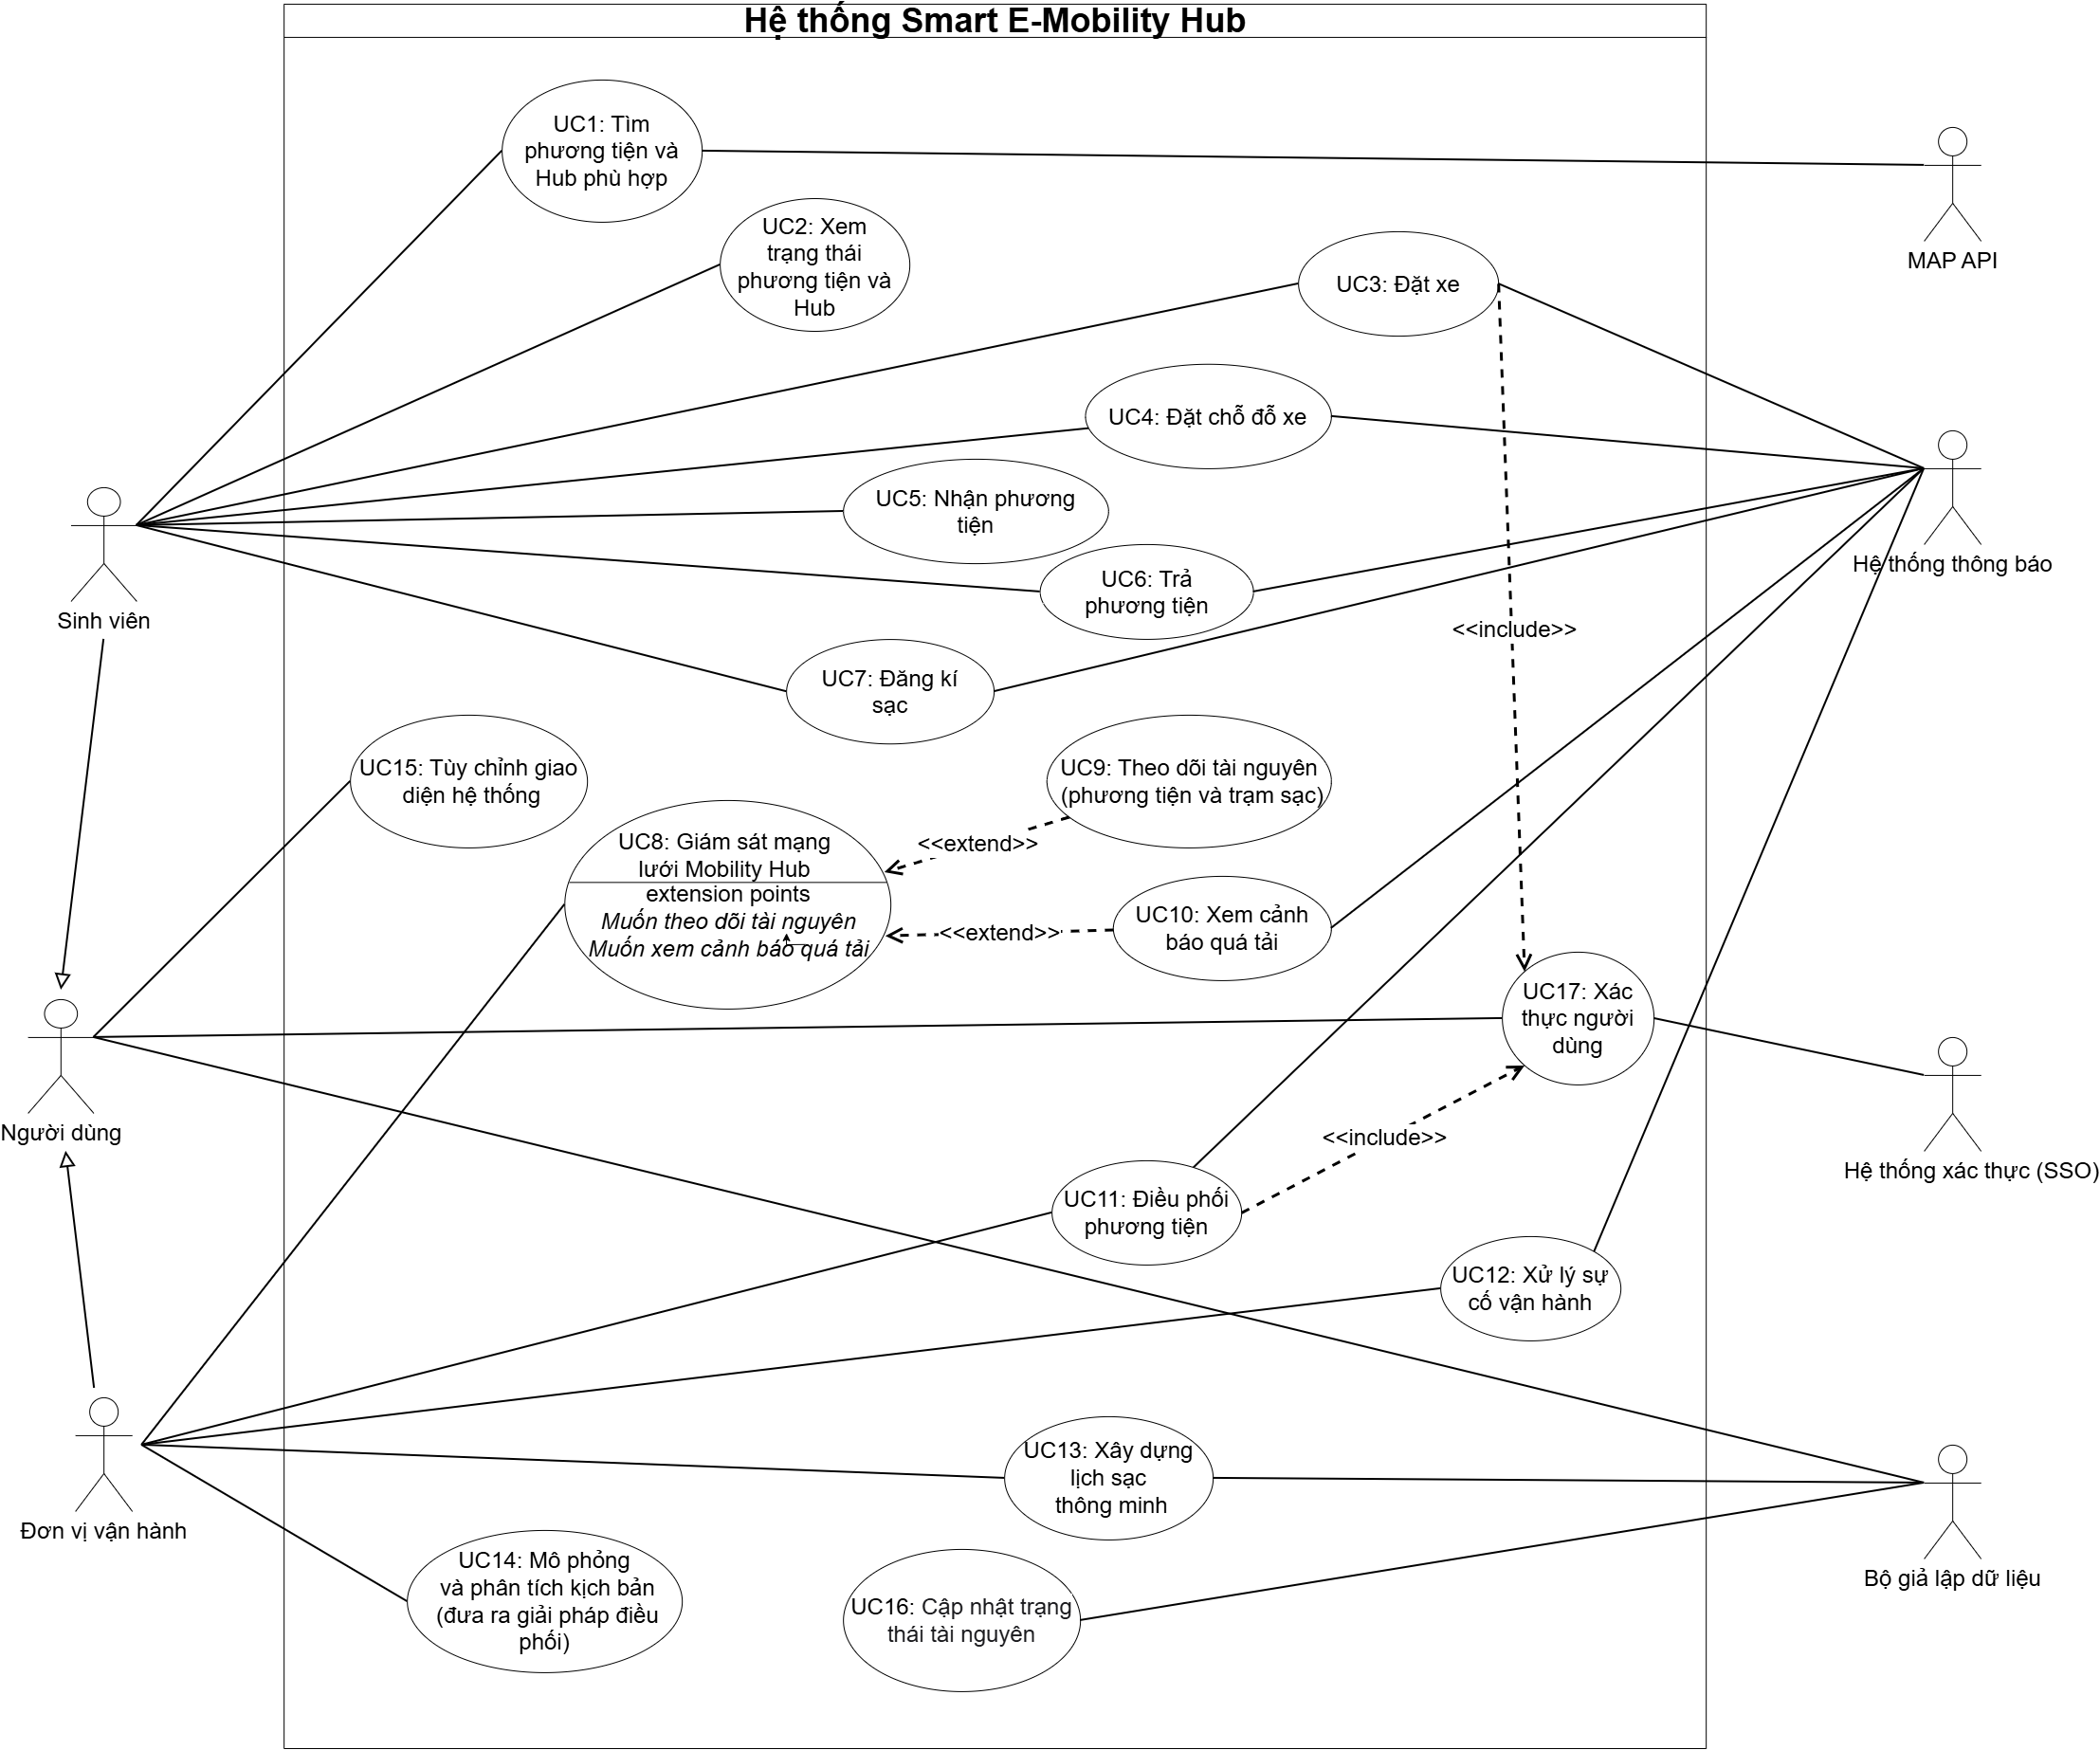
\includegraphics[width=0.98\textwidth,height=0.78\textheight,keepaspectratio]{s1/uc-diagram4.png}
\captionof{figure}{Sơ đồ Use Case của hệ thống Smart E-Mobility Hub}
\label{fig:usecase-diagram}
\end{center}
\noindent\textit{Ghi chú:} Actor Người dùng trên sơ đồ đóng vai trò là một Actor trừu tượng (\textit{Abstract Actor}), dùng để khái quát hóa quyền truy cập của cả Sinh viên và Đơn vị vận hành đối với các Use Case dùng chung.
\clearpage

\section{Đặc tả kịch bản Use Case (Use-case Scenarios)}

% Các bảng đặc tả được chuyển từ BBH BTL CNPM.pdf.

\subsection{Nhóm Use Case dành cho Sinh viên}

\subsubsection{UC1: Tìm phương tiện và Hub phù hợp}

{

\small

\setlength{\tabcolsep}{1pt}

\renewcommand{\arraystretch}{1.22}

\begin{longtable}{|>{\raggedright\arraybackslash}p{3.0cm}|>{\raggedright\arraybackslash}p{3.6cm}|>{\raggedright\arraybackslash}p{3.0cm}|>{\raggedright\arraybackslash}p{3.6cm}|}

\hline

\textbf{Field} & \multicolumn{3}{>{\raggedright\arraybackslash}p{10.2cm}|}{\textbf{Description}} \\

\hline

\endfirsthead

\hline

\textbf{Field} & \multicolumn{3}{>{\raggedright\arraybackslash}p{10.2cm}|}{\textbf{Description (tiếp theo)}} \\

\hline

\endhead

Use Case ID: & \multicolumn{3}{>{\raggedright\arraybackslash}p{10.2cm}|}{UC1} \\
\hline

Tên Use Case: & \multicolumn{3}{>{\raggedright\arraybackslash}p{10.2cm}|}{Tìm phương tiện và Hub phù hợp} \\
\hline

Tạo bởi: & Hoàng Phạm Tiến Thành & Lần cập nhật cuối bởi: & Hoàng Phạm Tiến Thành \\
\hline

Tạo vào ngày: & 18/09/2026 & Lần cập nhật cuối: & 19/09/2026 \\
\hline

Actors: & \multicolumn{3}{>{\raggedright\arraybackslash}p{10.2cm}|}{Sinh viên, Map API} \\
\hline

Mô tả: & \multicolumn{3}{>{\raggedright\arraybackslash}p{10.2cm}|}{Giúp sinh viên xác định các phương tiện điện dùng chung hoặc Mobility Hub phù hợp với vị trí và tiêu chí tìm kiếm, làm cơ sở để xem chi tiết hoặc thực hiện đặt tài nguyên.} \\
\hline

Trigger: & \multicolumn{3}{>{\raggedright\arraybackslash}p{10.2cm}|}{Sinh viên chọn chức năng “Tìm phương tiện và Hub”.} \\
\hline

Preconditions: & \multicolumn{3}{>{\raggedright\arraybackslash}p{10.2cm}|}{1. Sinh viên có thể truy cập giao diện tìm kiếm của hệ thống.\newline
2. Thông tin danh mục và tọa độ các Hub thuộc phạm vi phục vụ đã được cấu hình.\newline
3. Không bắt buộc sinh viên đăng nhập để thực hiện UC1.} \\
\hline

Postconditions: & \multicolumn{3}{>{\raggedright\arraybackslash}p{10.2cm}|}{1. Hệ thống hiển thị kết quả phù hợp với vị trí và tiêu chí đã chọn; hoặc thông báo không có kết quả phù hợp.\newline
2. Mỗi kết quả có thông tin tóm tắt và thời điểm cập nhật trạng thái để sinh viên đánh giá.\newline
3. Tiêu chí tìm kiếm được giữ trên giao diện để sinh viên điều chỉnh hoặc xem chi tiết kết quả.} \\
\hline

Normal Flow: & \multicolumn{3}{>{\raggedright\arraybackslash}p{10.2cm}|}{1. Sinh viên mở chức năng “Tìm phương tiện và Hub”.\newline
2. Hệ thống hiển thị giao diện tìm kiếm và bản đồ.\newline
3. Sinh viên chọn tìm phương tiện, sử dụng vị trí hiện tại và cấp quyền truy cập vị trí khi được yêu cầu.\newline
4. Hệ thống xác định và hiển thị vị trí tìm kiếm.\newline
5. Sinh viên chọn phạm vi khoảng cách, loại phương tiện, mức pin tối thiểu và gửi yêu cầu tìm kiếm.\newline
6. Hệ thống kiểm tra tính hợp lệ của thông tin, tìm các phương tiện khả dụng đáp ứng tiêu chí và sắp xếp theo khoảng cách đến Hub.\newline
7. Hệ thống hiển thị danh sách kết quả và vị trí Hub trên bản đồ, kèm thông tin tóm tắt về phương tiện, mức pin, trạng thái, khoảng cách và thời điểm cập nhật.\newline
8. Sinh viên xem kết quả. Use case kết thúc.} \\
\hline

Alternative Flows: & \multicolumn{3}{>{\raggedright\arraybackslash}p{10.2cm}|}{AF1: Tại bước 3, nhánh 3a --- Chọn vị trí thủ công. Sinh viên không sử dụng vị trí hiện tại hoặc từ chối cấp quyền định vị. Hệ thống cho phép chọn vị trí, khu vực hoặc Hub trên bản đồ; sau đó tiếp tục từ bước 4.\newline
AF2: Tại bước 3, nhánh 3b --- Tìm Hub thay vì tìm phương tiện. Hệ thống tìm theo khoảng cách, số xe khả dụng, số chỗ đỗ trống và số cổng sạc khả dụng; sau đó hiển thị kết quả Hub phù hợp.\newline
AF3: Tại bước 6, nhánh 6a --- Không có kết quả phù hợp. Hệ thống giữ điều kiện tìm kiếm và cho phép Sinh viên điều chỉnh rồi quay lại bước 5.\newline
AF4: Tại bước 7, nhánh 7a --- Điều chỉnh bộ lọc. Sinh viên thay đổi vị trí hoặc bộ lọc; hệ thống thực hiện lại từ bước 5.\newline
AF5: Tại bước 7, nhánh 7b --- Hủy tìm kiếm. Sinh viên rời khỏi màn hình tìm kiếm. Use case kết thúc, không thay đổi trạng thái tài nguyên.} \\
\hline

Exceptions: & \multicolumn{3}{>{\raggedright\arraybackslash}p{10.2cm}|}{EX1: Tại bước 3 --- Không xác định được vị trí. Thiết bị không cung cấp được tọa độ. Hệ thống thông báo lỗi và cho phép Sinh viên thử lại hoặc chuyển sang nhánh 3a.\newline
EX2: Tại bước 5 --- Tiêu chí tìm kiếm không hợp lệ. Hệ thống chỉ rõ thông tin cần chỉnh sửa và yêu cầu Sinh viên nhập lại trước khi quay lại bước 5.\newline
EX3: Tại bước 2 hoặc bước 7 --- Map API không khả dụng. Hệ thống thông báo lỗi bản đồ và chuyển sang hiển thị danh sách Hub theo khu vực hoặc tọa độ đã lưu.\newline
EX4: Tại bước 6 --- Không truy xuất được dữ liệu phương tiện/Hub hoặc mất kết nối. Hệ thống thông báo lỗi, giữ lại tiêu chí đã nhập và cho phép Sinh viên thử lại.} \\
\hline

FR liên quan: & \multicolumn{3}{>{\raggedright\arraybackslash}p{10.2cm}|}{FR01, FR13} \\
\hline
NFR liên quan: & \multicolumn{3}{>{\raggedright\arraybackslash}p{10.2cm}|}{NFR01, NFR02} \\
\hline
\end{longtable}

}

\clearpage

\subsubsection{UC2: Xem trạng thái phương tiện và Hub}

{

\small

\setlength{\tabcolsep}{1pt}

\renewcommand{\arraystretch}{1.22}

\begin{longtable}{|>{\raggedright\arraybackslash}p{3.0cm}|>{\raggedright\arraybackslash}p{3.6cm}|>{\raggedright\arraybackslash}p{3.0cm}|>{\raggedright\arraybackslash}p{3.6cm}|}

\hline

\textbf{Field} & \multicolumn{3}{>{\raggedright\arraybackslash}p{10.2cm}|}{\textbf{Description}} \\

\hline

\endfirsthead

\hline

\textbf{Field} & \multicolumn{3}{>{\raggedright\arraybackslash}p{10.2cm}|}{\textbf{Description (tiếp theo)}} \\

\hline

\endhead

Use Case ID: & \multicolumn{3}{>{\raggedright\arraybackslash}p{10.2cm}|}{UC2} \\
\hline

Tên Use Case: & \multicolumn{3}{>{\raggedright\arraybackslash}p{10.2cm}|}{Xem trạng thái phương tiện và Hub} \\
\hline

Tạo bởi: & Hoàng Phạm Tiến Thành & Lần cập nhật cuối bởi: & Hoàng Phạm Tiến Thành \\
\hline

Tạo vào ngày: & 18/09/2026 & Lần cập nhật cuối: & 19/09/2026 \\
\hline

Actors: & \multicolumn{3}{>{\raggedright\arraybackslash}p{10.2cm}|}{Sinh viên} \\
\hline

Mô tả: & \multicolumn{3}{>{\raggedright\arraybackslash}p{10.2cm}|}{Giúp Sinh viên xem trạng thái gần thời gian thực của một phương tiện hoặc Mobility Hub đã chọn để quyết định có tiếp tục tìm kiếm, đặt xe, đặt chỗ hoặc đăng ký sạc hay không.} \\
\hline

Trigger: & \multicolumn{3}{>{\raggedright\arraybackslash}p{10.2cm}|}{Sinh viên chọn chức năng “Xem trạng thái phương tiện và Hub” hoặc chọn một phương tiện/Hub từ kết quả của UC1.} \\
\hline

Preconditions: & \multicolumn{3}{>{\raggedright\arraybackslash}p{10.2cm}|}{1. Sinh viên có thể truy cập giao diện hệ thống.\newline
2. Phương tiện hoặc Hub cần xem có mã định danh trong hệ thống.\newline
3. Hệ thống có dữ liệu trạng thái gần nhất của tài nguyên hoặc có thể truy xuất dữ liệu đó.} \\
\hline

Postconditions: & \multicolumn{3}{>{\raggedright\arraybackslash}p{10.2cm}|}{1. Thành công: Hệ thống hiển thị trạng thái và thời điểm cập nhật gần nhất của tài nguyên được chọn.\newline
2. Thất bại hoặc hủy: Không có trạng thái tài nguyên, đơn đặt hoặc dữ liệu nào bị thay đổi.} \\
\hline

Normal Flow: & \multicolumn{3}{>{\raggedright\arraybackslash}p{10.2cm}|}{1. Sinh viên mở chức năng “Xem trạng thái phương tiện và Hub” hoặc chọn một phương tiện/Hub từ danh sách kết quả.\newline
2. Hệ thống xác định loại tài nguyên được chọn và truy xuất trạng thái gần nhất cùng thời điểm cập nhật.\newline
3. Hệ thống hiển thị thông tin chi tiết. Với phương tiện: loại xe, trạng thái, mức pin và Hub hiện tại. Với Hub: số phương tiện khả dụng, số chỗ đỗ trống, số cổng sạc khả dụng, mức độ sử dụng và thời điểm cập nhật.\newline
4. Sinh viên xem thông tin trạng thái. Use case kết thúc.} \\
\hline

Alternative Flows: & \multicolumn{3}{>{\raggedright\arraybackslash}p{10.2cm}|}{AF1: Tại bước 1, nhánh 1a --- Chọn xem phương tiện. Hệ thống hiển thị loại xe, trạng thái, mức pin và Hub hiện tại theo bước 2 và bước 3.\newline
AF2: Tại bước 1, nhánh 1b --- Chọn xem Hub. Hệ thống hiển thị số phương tiện khả dụng, chỗ đỗ trống, cổng sạc khả dụng và mức độ sử dụng theo bước 2 và bước 3.\newline
AF3: Tại bước 3, nhánh 3a --- Làm mới thông tin. Hệ thống truy xuất lại trạng thái gần nhất và thực hiện lại từ bước 2.\newline
AF4: Tại bước 3, nhánh 3b --- Tài nguyên không khả dụng. Hệ thống vẫn hiển thị trạng thái hiện tại, thời điểm cập nhật và cho phép Sinh viên chọn tài nguyên khác.\newline
AF5: Tại bước 3, nhánh 3c --- Chọn tài nguyên khác. Hệ thống thực hiện lại từ bước 1.\newline
AF6: Tại bước 4, nhánh 4a --- Rời màn hình. Use case kết thúc mà không thay đổi dữ liệu.} \\
\hline

Exceptions: & \multicolumn{3}{>{\raggedright\arraybackslash}p{10.2cm}|}{EX1: Tại bước 1 --- Chưa chọn tài nguyên hợp lệ. Hệ thống yêu cầu Sinh viên chọn phương tiện hoặc Hub trước khi tiếp tục.\newline
EX2: Tại bước 2 --- Tài nguyên không còn tồn tại hoặc đã ngừng hoạt động. Hệ thống thông báo và đưa Sinh viên về danh sách tìm kiếm hoặc danh sách tài nguyên.\newline
EX3: Tại bước 2 --- Không truy xuất được dữ liệu trạng thái. Hệ thống thông báo lỗi, giữ lại tài nguyên đang chọn và cho phép Sinh viên thử lại.\newline
EX4: Tại bước 2 --- Dữ liệu quá cũ hoặc chưa xác định. Hệ thống hiển thị thời điểm cập nhật gần nhất, đánh dấu dữ liệu chưa đáng tin cậy và không khẳng định tài nguyên còn khả dụng.} \\
\hline

FR liên quan: & \multicolumn{3}{>{\raggedright\arraybackslash}p{10.2cm}|}{FR02} \\
\hline
NFR liên quan: & \multicolumn{3}{>{\raggedright\arraybackslash}p{10.2cm}|}{NFR02} \\
\hline
\end{longtable}

}

\clearpage

\subsubsection{UC3: Đặt xe}

{

\small

\setlength{\tabcolsep}{1pt}

\renewcommand{\arraystretch}{1.22}

\begin{longtable}{|>{\raggedright\arraybackslash}p{3.0cm}|>{\raggedright\arraybackslash}p{3.6cm}|>{\raggedright\arraybackslash}p{3.0cm}|>{\raggedright\arraybackslash}p{3.6cm}|}

\hline

\textbf{Field} & \multicolumn{3}{>{\raggedright\arraybackslash}p{10.2cm}|}{\textbf{Description}} \\

\hline

\endfirsthead

\hline

\textbf{Field} & \multicolumn{3}{>{\raggedright\arraybackslash}p{10.2cm}|}{\textbf{Description (tiếp theo)}} \\

\hline

\endhead

Use Case ID: & \multicolumn{3}{>{\raggedright\arraybackslash}p{10.2cm}|}{UC3} \\
\hline

Tên Use Case: & \multicolumn{3}{>{\raggedright\arraybackslash}p{10.2cm}|}{Đặt xe} \\
\hline

Tạo bởi: & Nguyễn Khang Kỳ & Lần cập nhật cuối bởi: & Nguyễn Khang Kỳ \\
\hline

Tạo vào ngày: & 18/09/2026 & Lần cập nhật cuối: & 19/09/2026 \\
\hline

Actors: & \multicolumn{3}{>{\raggedright\arraybackslash}p{10.2cm}|}{Sinh viên; Hệ thống SSO; Hệ thống thông báo.} \\
\hline

Mô tả: & \multicolumn{3}{>{\raggedright\arraybackslash}p{10.2cm}|}{Sinh viên đặt trước phương tiện điện dùng chung tại Mobility Hub để có xe phục vụ hành trình di chuyển.} \\
\hline

Trigger: & \multicolumn{3}{>{\raggedright\arraybackslash}p{10.2cm}|}{Sinh viên chọn chức năng “Đặt xe” đối với phương tiện mong muốn.} \\
\hline

Preconditions: & \multicolumn{3}{>{\raggedright\arraybackslash}p{10.2cm}|}{1. Sinh viên có tài khoản SSO được phép sử dụng dịch vụ.\newline
2. Phương tiện và Hub đã có thông tin trên hệ thống.\newline
3. Sinh viên đã chọn một phương tiện cụ thể từ kết quả của UC1/UC2.} \\
\hline

Postconditions: & \multicolumn{3}{>{\raggedright\arraybackslash}p{10.2cm}|}{1. Thông tin đặt xe được lưu và gắn với sinh viên.\newline
2. Phương tiện chuyển sang trạng thái “Đã đặt”.\newline
3. Sinh viên nhận được thông tin xác nhận đặt xe.\newline
4. Nếu thất bại, không tạo đơn đặt và xe không bị giữ ở trạng thái không chính xác.} \\
\hline

Normal Flow: & \multicolumn{3}{>{\raggedright\arraybackslash}p{10.2cm}|}{1. Sinh viên chọn phương tiện và yêu cầu đặt xe.\newline
2. Hệ thống kiểm tra phiên làm việc hợp lệ và quyền sử dụng dịch vụ hợp lệ.\newline
3. Hệ thống hiển thị thông tin xe, mức pin và Hub nhận xe.\newline
4. Sinh viên kiểm tra thông tin và xác nhận đặt xe.\newline
5. Hệ thống thực hiện giao dịch nguyên tử: kiểm tra khả dụng, tạo đơn đặt, chuyển xe sang “Đã đặt” và ghi log.\newline
6. Hệ thống xác nhận giao dịch hoàn tất.\newline
7. Hệ thống hiển thị kết quả và, khi cần gửi ngoài ứng dụng, chuyển yêu cầu xác nhận đến Hệ thống thông báo.} \\
\hline

Alternative Flows: & \multicolumn{3}{>{\raggedright\arraybackslash}p{10.2cm}|}{AF1: Chọn phương tiện khác tại bước 3.\newline
3a. Sinh viên quay lại danh sách và chọn xe khác.\newline
3b. Hệ thống hiển thị thông tin phương tiện mới. Tiếp tục bước 4 của luồng chính.\newline
AF2: Hủy thao tác trước khi xác nhận tại bước 4.\newline
4a. Sinh viên chọn hủy đặt xe.\newline
4b. Hệ thống bỏ lựa chọn chưa lưu, không giữ xe. Use case kết thúc; không tạo đặt xe mới.} \\
\hline

Exceptions: & \multicolumn{3}{>{\raggedright\arraybackslash}p{10.2cm}|}{EX1: EX1: Phiên làm việc không hợp lệ hoặc đã hết hạn tại bước 2.\newline
2a. Hệ thống phát hiện phiên đăng nhập không còn hiệu lực.\newline
2b. Hệ thống lưu tạm lựa chọn phương tiện của sinh viên và thông báo yêu cầu xác thực.\newline
2c. Hệ thống tự động chuyển hướng người dùng sang màn hình đăng nhập (UC17).\newline
2d. Nếu xác thực thành công, hệ thống điều hướng sinh viên quay lại tiếp tục từ bước 3 của luồng chính. Nếu xác thực thất bại hoặc người dùng hủy, hệ thống xóa dữ liệu chọn xe tạm thời. Use case kết thúc.\newline
EX2: Xe không còn khả dụng tại bước 5.\newline
5a. Hệ thống thông báo xe đã được đặt, đang sử dụng hoặc không thể phục vụ.\newline
5b. Hệ thống làm mới danh sách để sinh viên chọn xe khác. Quay lại bước 1 hoặc kết thúc nếu sinh viên không tiếp tục.\newline
EX3: Không lưu được đặt xe tại bước 6.\newline
6a. Hệ thống thông báo chưa hoàn tất đặt xe.\newline
6b. Hệ thống kiểm tra kết quả lưu trước khi cho thử lại để tránh đặt trùng. Không xác nhận thành công khi chưa lưu được đặt xe.} \\
\hline

FR liên quan: & \multicolumn{3}{>{\raggedright\arraybackslash}p{10.2cm}|}{FR03, FR14} \\
\hline
NFR liên quan: & \multicolumn{3}{>{\raggedright\arraybackslash}p{10.2cm}|}{NFR09, NFR10, NFR11, NFR12} \\
\hline

\end{longtable}

}

\clearpage

\subsubsection{UC4: Đặt chỗ đỗ xe}

{

\small

\setlength{\tabcolsep}{1pt}

\renewcommand{\arraystretch}{1.22}

\begin{longtable}{|>{\raggedright\arraybackslash}p{3.0cm}|>{\raggedright\arraybackslash}p{3.6cm}|>{\raggedright\arraybackslash}p{3.0cm}|>{\raggedright\arraybackslash}p{3.6cm}|}

\hline

\textbf{Field} & \multicolumn{3}{>{\raggedright\arraybackslash}p{10.2cm}|}{\textbf{Description}} \\

\hline

\endfirsthead

\hline

\textbf{Field} & \multicolumn{3}{>{\raggedright\arraybackslash}p{10.2cm}|}{\textbf{Description (tiếp theo)}} \\

\hline

\endhead

Use Case ID: & \multicolumn{3}{>{\raggedright\arraybackslash}p{10.2cm}|}{UC4} \\
\hline

Tên Use Case: & \multicolumn{3}{>{\raggedright\arraybackslash}p{10.2cm}|}{Đặt chỗ đỗ xe} \\
\hline

Tạo bởi: & Nguyễn Khang Kỳ & Lần cập nhật cuối bởi: & Nguyễn Khang Kỳ \\
\hline

Tạo vào ngày: & 18/09/2026 & Lần cập nhật cuối: & 19/09/2026 \\
\hline

Actors: & \multicolumn{3}{>{\raggedright\arraybackslash}p{10.2cm}|}{Sinh viên; Hệ thống thông báo.} \\
\hline

Mô tả: & \multicolumn{3}{>{\raggedright\arraybackslash}p{10.2cm}|}{Sinh viên sử dụng phương tiện điện cá nhân đặt trước chỗ đỗ tại Mobility Hub để có vị trí đỗ phù hợp khi đến nơi.} \\
\hline

Trigger: & \multicolumn{3}{>{\raggedright\arraybackslash}p{10.2cm}|}{Sinh viên chọn chức năng “Đặt chỗ đỗ xe”.} \\
\hline

Preconditions: & \multicolumn{3}{>{\raggedright\arraybackslash}p{10.2cm}|}{1. Sinh viên có phiên đăng nhập hợp lệ và có quyền đặt chỗ.\newline
2. Thông tin Hub và chỗ đỗ đã được cấu hình trên hệ thống.\newline
3. Phương tiện cá nhân hoặc nhu cầu đỗ cần thiết đã được xác định.} \\
\hline

Postconditions: & \multicolumn{3}{>{\raggedright\arraybackslash}p{10.2cm}|}{1. Thông tin đặt chỗ được lưu cho sinh viên.\newline
2. Chỗ đỗ được giữ trong khoảng thời gian đã chọn.\newline
3. Thông tin chỗ đỗ và kết quả đăng ký được cập nhật trên hệ thống.} \\
\hline

Normal Flow: & \multicolumn{3}{>{\raggedright\arraybackslash}p{10.2cm}|}{1. Sinh viên chọn chức năng “Đặt chỗ đỗ xe”.\newline
2. Hệ thống hiển thị các Hub và thông tin chỗ đỗ.\newline
3. Sinh viên chọn Hub, vị trí đỗ và khoảng thời gian cần sử dụng.\newline
4. Hệ thống kiểm tra dữ liệu thời gian và hiển thị thông tin để xác nhận.\newline
5. Sinh viên xác nhận đặt chỗ.\newline
6. Hệ thống thực hiện giao dịch nguyên tử: kiểm tra lại khả dụng, lưu đặt chỗ, giữ vị trí trong khoảng thời gian đã chọn và ghi log.\newline
7. Hệ thống hiển thị kết quả và, khi cần gửi ngoài ứng dụng, chuyển yêu cầu xác nhận đến Hệ thống thông báo.} \\
\hline

Alternative Flows: & \multicolumn{3}{>{\raggedright\arraybackslash}p{10.2cm}|}{AF1: Thay đổi lựa chọn tại bước 4.\newline
4a. Sinh viên chọn thay đổi Hub, chỗ đỗ hoặc thời gian.\newline
4b. Hệ thống hiển thị lại các lựa chọn phù hợp. Quay lại bước 3 của luồng chính.\newline
AF2: Hủy thao tác trước khi xác nhận tại bước 5.\newline
5a. Sinh viên chọn hủy yêu cầu.\newline
5b. Hệ thống không lưu đăng ký mới và không giữ chỗ đỗ. Use case kết thúc.} \\
\hline

Exceptions: & \multicolumn{3}{>{\raggedright\arraybackslash}p{10.2cm}|}{EX1: Không còn chỗ phù hợp tại bước 4 hoặc 6.\newline
4a. Hệ thống thông báo chỗ đã được đặt hoặc không còn khả dụng trong khoảng thời gian yêu cầu.\newline
4b. Sinh viên có thể chọn chỗ khác, đổi Hub hoặc thời gian. Quay lại bước 3; kết thúc nếu sinh viên không tiếp tục.\newline
EX2: Khoảng thời gian không hợp lệ tại bước 4.\newline
4a. Hệ thống thông báo thời gian không hợp lệ, chẳng hạn thời điểm kết thúc trước thời điểm bắt đầu.\newline
4b. Sinh viên nhập lại thời gian. Quay lại bước 3 của luồng chính.\newline
EX3: Không lưu được đăng ký tại bước 6.\newline
6a. Hệ thống thông báo chưa hoàn tất đặt chỗ.\newline
6b. Hệ thống kiểm tra kết quả lưu trước khi cho sinh viên thử lại. Không xác nhận giữ chỗ nếu đăng ký chưa được lưu.} \\
\hline

FR liên quan: & \multicolumn{3}{>{\raggedright\arraybackslash}p{10.2cm}|}{FR03, FR14} \\
\hline
NFR liên quan: & \multicolumn{3}{>{\raggedright\arraybackslash}p{10.2cm}|}{NFR09, NFR10, NFR11, NFR12} \\
\hline

\end{longtable}

}

\clearpage

\subsubsection{UC5: Nhận phương tiện}

{

\small

\setlength{\tabcolsep}{1pt}

\renewcommand{\arraystretch}{1.22}

\begin{longtable}{|>{\raggedright\arraybackslash}p{3.0cm}|>{\raggedright\arraybackslash}p{3.6cm}|>{\raggedright\arraybackslash}p{3.0cm}|>{\raggedright\arraybackslash}p{3.6cm}|}

\hline

\textbf{Field} & \multicolumn{3}{>{\raggedright\arraybackslash}p{10.2cm}|}{\textbf{Description}} \\

\hline

\endfirsthead

\hline

\textbf{Field} & \multicolumn{3}{>{\raggedright\arraybackslash}p{10.2cm}|}{\textbf{Description (tiếp theo)}} \\

\hline

\endhead

Use Case ID: & \multicolumn{3}{>{\raggedright\arraybackslash}p{10.2cm}|}{UC5} \\
\hline

Tên Use Case: & \multicolumn{3}{>{\raggedright\arraybackslash}p{10.2cm}|}{Nhận phương tiện} \\
\hline

Tạo bởi: & Nguyễn Khang Kỳ & Lần cập nhật cuối bởi: & Nguyễn Khang Kỳ \\
\hline

Tạo vào ngày: & 18/09/2026 & Lần cập nhật cuối: & 19/09/2026 \\
\hline

Actors: & \multicolumn{3}{>{\raggedright\arraybackslash}p{10.2cm}|}{Sinh viên.} \\
\hline

Mô tả: & \multicolumn{3}{>{\raggedright\arraybackslash}p{10.2cm}|}{Sinh viên nhận phương tiện điện dùng chung đã đặt tại Mobility Hub để bắt đầu chuyến đi.} \\
\hline

Trigger: & \multicolumn{3}{>{\raggedright\arraybackslash}p{10.2cm}|}{Sinh viên chọn chức năng “Nhận phương tiện” trong thông tin đặt xe.} \\
\hline

Preconditions: & \multicolumn{3}{>{\raggedright\arraybackslash}p{10.2cm}|}{1. Sinh viên đã đăng nhập vào hệ thống.\newline
2. Sinh viên đã có thông tin đặt xe từ UC3.} \\
\hline

Postconditions: & \multicolumn{3}{>{\raggedright\arraybackslash}p{10.2cm}|}{1. Hệ thống ghi nhận sinh viên đã nhận đúng phương tiện.\newline
2. Trạng thái phương tiện chuyển sang “Đang sử dụng”; đặt xe chuyển sang “Đã nhận”.\newline
3. Thời điểm nhận xe và người nhận được lưu trên hệ thống.} \\
\hline

Normal Flow: & \multicolumn{3}{>{\raggedright\arraybackslash}p{10.2cm}|}{1. Sinh viên mở thông tin đặt xe và chọn “Nhận phương tiện”.\newline
2. Hệ thống kiểm tra người đặt, hiệu lực đặt xe, Hub nhận và trạng thái phương tiện.\newline
3. Sinh viên xác nhận đã nhận phương tiện trên giao diện; hệ thống chỉ mô phỏng và ghi nhận thao tác nhận, không điều khiển khóa vật lý.\newline
4. Hệ thống cập nhật xe sang “Đang sử dụng”, đặt xe sang “Đã nhận”, lưu thời điểm nhận và ghi log.\newline
5. Sau khi cập nhật thành công, hệ thống hiển thị xác nhận hoàn tất.} \\
\hline

Alternative Flows: & \multicolumn{3}{>{\raggedright\arraybackslash}p{10.2cm}|}{AF1: Chọn lại thông tin đặt xe tại bước 2.\newline
2a. Sinh viên quay lại danh sách đặt xe của mình.\newline
2b. Sinh viên chọn đúng đặt xe muốn nhận. Tiếp tục bước 2 để kiểm tra.\newline
AF2: Hủy yêu cầu nhận trước khi xác nhận tại bước 3.\newline
3a. Sinh viên chọn không tiếp tục nhận xe.\newline
3b. Hệ thống dừng thao tác nhận; đặt xe hiện có không bị hủy. Use case kết thúc; xe chưa chuyển sang “Đang sử dụng”.} \\
\hline

Exceptions: & \multicolumn{3}{>{\raggedright\arraybackslash}p{10.2cm}|}{EX1: Đặt xe không hợp lệ tại bước 2.\newline
2a. Hệ thống thông báo đặt xe không tồn tại, không thuộc sinh viên hoặc không còn hiệu lực.\newline
2b. Hệ thống không cho phép nhận phương tiện. Use case kết thúc.\newline
EX2: Phương tiện không thể nhận tại bước 2 hoặc 3.\newline
2a. Hệ thống thông báo xe không khả dụng hoặc có sự cố theo dữ liệu mô phỏng.\newline
2b. Sinh viên được hướng dẫn liên hệ đơn vị vận hành. Use case kết thúc; không ghi nhận nhận xe thành công.\newline
EX3: Lỗi cập nhật trạng thái tại bước 5.\newline
5a. Hệ thống thông báo quá trình nhận xe chưa hoàn tất cập nhật.\newline
5b. Hệ thống giữ thông tin nhận đã ghi, không cho người khác đặt xe này và chuyển đơn vị vận hành kiểm tra. Chưa xác nhận hoàn tất cho đến khi cập nhật thành công.} \\
\hline

FR liên quan: & \multicolumn{3}{>{\raggedright\arraybackslash}p{10.2cm}|}{FR03} \\
\hline
NFR liên quan: & \multicolumn{3}{>{\raggedright\arraybackslash}p{10.2cm}|}{NFR10, NFR11, NFR12} \\
\hline

\end{longtable}

}

\clearpage

\subsubsection{UC6: Trả phương tiện}

{

\small

\setlength{\tabcolsep}{1pt}

\renewcommand{\arraystretch}{1.22}

\begin{longtable}{|>{\raggedright\arraybackslash}p{3.0cm}|>{\raggedright\arraybackslash}p{3.6cm}|>{\raggedright\arraybackslash}p{3.0cm}|>{\raggedright\arraybackslash}p{3.6cm}|}

\hline

\textbf{Field} & \multicolumn{3}{>{\raggedright\arraybackslash}p{10.2cm}|}{\textbf{Description}} \\

\hline

\endfirsthead

\hline

\textbf{Field} & \multicolumn{3}{>{\raggedright\arraybackslash}p{10.2cm}|}{\textbf{Description (tiếp theo)}} \\

\hline

\endhead

Use Case ID: & \multicolumn{3}{>{\raggedright\arraybackslash}p{10.2cm}|}{UC6} \\
\hline

Tên Use Case: & \multicolumn{3}{>{\raggedright\arraybackslash}p{10.2cm}|}{Trả phương tiện} \\
\hline

Tạo bởi: & Võ Tấn Phát & Lần cập nhật cuối bởi: & Võ Tấn Phát \\
\hline

Tạo vào ngày: & 18/09/2026 & Lần cập nhật cuối: & 19/09/2026 \\
\hline

Actors: & \multicolumn{3}{>{\raggedright\arraybackslash}p{10.2cm}|}{Sinh viên, Hệ thống thông báo} \\
\hline

Mô tả: & \multicolumn{3}{>{\raggedright\arraybackslash}p{10.2cm}|}{Sinh viên trả phương tiện về cho hệ thống Smart Mobility Hub. Hệ thống thông báo sẽ cho biết phương tiện đã được trả về và có thể được mượn cho những người dùng khác.} \\
\hline

Trigger: & \multicolumn{3}{>{\raggedright\arraybackslash}p{10.2cm}|}{Sinh viên đưa phương tiện về Smart Mobility Hub và thực hiện chức năng “Trả phương tiện”.} \\
\hline

Preconditions: & \multicolumn{3}{>{\raggedright\arraybackslash}p{10.2cm}|}{1. Sinh viên có phiên đăng nhập hợp lệ và là người đang sử dụng phương tiện.\newline
2. Phương tiện đang được mượn và chưa được trả về.\newline
3. Hub nhận có khả năng tiếp nhận hoặc Sinh viên có chỗ đỗ đã đặt.} \\
\hline

Postconditions: & \multicolumn{3}{>{\raggedright\arraybackslash}p{10.2cm}|}{1. Phương tiện được đưa về trạng thái có sẵn trên hệ thống.\newline
2. Lượt mượn của sinh viên kết thúc.\newline
3. Hệ thống thông báo phương tiện đã được trả về thành công.} \\
\hline

Normal Flow: & \multicolumn{3}{>{\raggedright\arraybackslash}p{10.2cm}|}{1. Sinh viên đưa phương tiện về trạm Mobility Hub.\newline
2. Sinh viên thực hiện chức năng “Trả phương tiện”.\newline
3. Hệ thống kiểm tra người sử dụng, thông tin phương tiện, lượt mượn và khả năng tiếp nhận tại Hub.\newline
4. Hệ thống thực hiện giao dịch trả xe, lưu thời điểm, người trả, phương tiện và Hub nhận vào audit log.\newline
5. Hệ thống kết thúc lượt mượn.\newline
6. Hệ thống cập nhật trạng thái xe sang “Có sẵn”, “Chờ sạc” hoặc “Bảo trì” tùy mức pin và trạng thái kỹ thuật.\newline
7. Sau khi giao dịch thành công, hệ thống hiển thị và, khi cần gửi ngoài ứng dụng, gửi xác nhận trả phương tiện.} \\
\hline

Alternative Flows: & \multicolumn{3}{>{\raggedright\arraybackslash}p{10.2cm}|}{Không có.} \\
\hline

Exceptions: & \multicolumn{3}{>{\raggedright\arraybackslash}p{10.2cm}|}{EX1: Hệ thống không nhận diện được phương tiện hoặc không phát hiện lượt mượn tại bước 3.\newline
3a. Hệ thống thông báo phương tiện không hợp lệ.\newline
3b. Hệ thống yêu cầu sinh viên kiểm tra lại phương tiện và liên hệ đơn vị vận hành để hỗ trợ.\newline
3c. Hệ thống hủy yêu cầu trả phương tiện. Use case kết thúc.\newline
EX2: Hệ thống gặp lỗi kết nối mạng tại bước 4.\newline
4a. Hệ thống thông báo lỗi ghi nhận việc trả phương tiện không thành công.\newline
4b. Hệ thống yêu cầu sinh viên thử lại sau ít phút. Use case kết thúc; không ghi nhận việc trả phương tiện.\newline
EX3: Không thể gửi thông báo trả phương tiện tại bước 7.\newline
7a. Hệ thống ghi nhận thành công việc trả phương tiện.\newline
7b. Hệ thống ghi nhận lỗi thông báo và xử lý lại. Use case kết thúc; việc ghi nhận trả phương tiện vẫn thành công.} \\
\hline

FR liên quan: & \multicolumn{3}{>{\raggedright\arraybackslash}p{10.2cm}|}{FR03, FR14} \\
\hline
NFR liên quan: & \multicolumn{3}{>{\raggedright\arraybackslash}p{10.2cm}|}{NFR10, NFR11, NFR12} \\
\hline
\end{longtable}

}

\clearpage

\subsubsection{UC7: Đăng ký sạc}

{

\small

\setlength{\tabcolsep}{1pt}

\renewcommand{\arraystretch}{1.22}

\begin{longtable}{|>{\raggedright\arraybackslash}p{3.0cm}|>{\raggedright\arraybackslash}p{3.6cm}|>{\raggedright\arraybackslash}p{3.0cm}|>{\raggedright\arraybackslash}p{3.6cm}|}

\hline

\textbf{Field} & \multicolumn{3}{>{\raggedright\arraybackslash}p{10.2cm}|}{\textbf{Description}} \\

\hline

\endfirsthead

\hline

\textbf{Field} & \multicolumn{3}{>{\raggedright\arraybackslash}p{10.2cm}|}{\textbf{Description (tiếp theo)}} \\

\hline

\endhead

Use Case ID: & \multicolumn{3}{>{\raggedright\arraybackslash}p{10.2cm}|}{UC7} \\
\hline

Tên Use Case: & \multicolumn{3}{>{\raggedright\arraybackslash}p{10.2cm}|}{Đăng ký sạc} \\
\hline

Tạo bởi: & Võ Tấn Phát & Lần cập nhật cuối bởi: & Võ Tấn Phát \\
\hline

Tạo vào ngày: & 18/09/2026 & Lần cập nhật cuối: & 19/09/2026 \\
\hline

Actors: & \multicolumn{3}{>{\raggedright\arraybackslash}p{10.2cm}|}{Sinh viên; Hệ thống thông báo.} \\
\hline

Mô tả: & \multicolumn{3}{>{\raggedright\arraybackslash}p{10.2cm}|}{Sinh viên yêu cầu đăng ký lịch sạc cho phương tiện điện tại hệ thống Smart Mobility Hub.} \\
\hline

Trigger: & \multicolumn{3}{>{\raggedright\arraybackslash}p{10.2cm}|}{Sinh viên sử dụng chức năng “Đăng ký sạc”.} \\
\hline

Preconditions: & \multicolumn{3}{>{\raggedright\arraybackslash}p{10.2cm}|}{1. Sinh viên có phiên đăng nhập hợp lệ.\newline
2. Phương tiện cần sạc đã được khai báo hoặc đang thuộc lượt sử dụng hợp lệ của Sinh viên.\newline
3. Dữ liệu cổng sạc và khung giờ đã được cập nhật trong hệ thống.} \\
\hline

Postconditions: & \multicolumn{3}{>{\raggedright\arraybackslash}p{10.2cm}|}{1. Yêu cầu đăng ký sạc được lưu vào hệ thống.\newline
2. Vị trí sạc được đăng ký cho sinh viên theo thời gian đã chọn.\newline
3. Thông tin đăng ký sạc được cập nhật trên hệ thống.} \\
\hline

Normal Flow: & \multicolumn{3}{>{\raggedright\arraybackslash}p{10.2cm}|}{1. Sinh viên chọn chức năng “Đăng ký sạc”.\newline
2. Hệ thống hiển thị thông tin đăng ký sạc.\newline
3. Sinh viên xác nhận nhu cầu sạc.\newline
4. Hệ thống hiển thị các cổng sạc và mốc thời gian khả dụng.\newline
5. Sinh viên chọn cổng sạc và thời gian sạc.\newline
6. Hệ thống hiển thị lịch sạc để Sinh viên xác nhận.\newline
7. Sinh viên xác nhận đăng ký sạc.\newline
8. Hệ thống thực hiện giao dịch nguyên tử: kiểm tra lại khung giờ, tạo đăng ký, giữ cổng sạc và ghi audit log.\newline
9. Sau khi giao dịch hoàn tất, hệ thống hiển thị xác nhận và chuyển yêu cầu đến Hệ thống thông báo.} \\
\hline

Alternative Flows: & \multicolumn{3}{>{\raggedright\arraybackslash}p{10.2cm}|}{AF1: Tại bước 5 --- Sinh viên thay đổi cổng sạc hoặc thời gian. Hệ thống hiển thị lại các lựa chọn khả dụng; Sinh viên chọn lại và tiếp tục từ bước 6.\newline
AF2: Tại bước 6 --- Sinh viên hủy yêu cầu trước khi xác nhận. Hệ thống không lưu đăng ký hoặc giữ cổng sạc. Use case kết thúc.\newline
AF3: Tại bước 1 --- Sinh viên yêu cầu sạc khẩn cấp cho phương tiện đang sử dụng. Hệ thống lấy vị trí hiện tại, đề xuất Hub gần nhất có cổng sạc; sau khi Sinh viên xác nhận, hệ thống giữ cổng sạc và gửi xác nhận. Use case kết thúc.} \\
\hline

Exceptions: & \multicolumn{3}{>{\raggedright\arraybackslash}p{10.2cm}|}{EX1: Tại bước 4 --- Không còn cổng sạc hoặc khung giờ khả dụng. Hệ thống thông báo và cho phép Sinh viên thử lại sau.\newline
EX2: Tại bước 8 --- Khung giờ vừa được người khác đặt. Hệ thống trả về xung đột, không tạo đăng ký trùng và gợi ý cổng sạc, khung giờ hoặc Hub khác.\newline
EX3: Tại bước 8 --- Không thể lưu đăng ký. Hệ thống hủy các thay đổi tạm thời, ghi log lỗi và không xác nhận thành công.} \\
\hline

FR liên quan: & \multicolumn{3}{>{\raggedright\arraybackslash}p{10.2cm}|}{FR04, FR14} \\
\hline
NFR liên quan: & \multicolumn{3}{>{\raggedright\arraybackslash}p{10.2cm}|}{NFR09, NFR10, NFR11, NFR12} \\
\hline
\end{longtable}

}

\clearpage

\subsection{Nhóm Use Case dành cho Đơn vị vận hành}

\subsubsection{UC8: Giám sát mạng lưới Mobility Hub (Base Use Case)}

{

\small

\setlength{\tabcolsep}{1pt}

\renewcommand{\arraystretch}{1.22}

\begin{longtable}{|>{\raggedright\arraybackslash}p{3.0cm}|>{\raggedright\arraybackslash}p{3.6cm}|>{\raggedright\arraybackslash}p{3.0cm}|>{\raggedright\arraybackslash}p{3.6cm}|}

\hline

\textbf{Field} & \multicolumn{3}{>{\raggedright\arraybackslash}p{10.2cm}|}{\textbf{Description}} \\

\hline

\endfirsthead

\hline

\textbf{Field} & \multicolumn{3}{>{\raggedright\arraybackslash}p{10.2cm}|}{\textbf{Description (tiếp theo)}} \\

\hline

\endhead

Use Case ID: & \multicolumn{3}{>{\raggedright\arraybackslash}p{10.2cm}|}{UC8} \\
\hline

Tên Use Case: & \multicolumn{3}{>{\raggedright\arraybackslash}p{10.2cm}|}{Giám sát mạng lưới Mobility Hub} \\
\hline

Tạo bởi: & Hoàng Phạm Tiến Thành & Lần cập nhật cuối bởi: & Hoàng Phạm Tiến Thành \\
\hline

Tạo vào ngày: & 18/09/2026 & Lần cập nhật cuối: & 19/09/2026 \\
\hline

Actors: & \multicolumn{3}{>{\raggedright\arraybackslash}p{10.2cm}|}{Đơn vị vận hành} \\
\hline

Mô tả: & \multicolumn{3}{>{\raggedright\arraybackslash}p{10.2cm}|}{Cung cấp cho Đơn vị vận hành cái nhìn tổng quan, gần thời gian thực về tình trạng của toàn bộ mạng lưới Mobility Hub để đánh giá mức độ sử dụng và quyết định có cần theo dõi chi tiết, xem cảnh báo hoặc thực hiện các hoạt động điều phối hay không.} \\
\hline

Trigger: & \multicolumn{3}{>{\raggedright\arraybackslash}p{10.2cm}|}{Đơn vị vận hành chọn chức năng “Giám sát mạng lưới Mobility Hub” trên hệ thống.} \\
\hline

Preconditions: & \multicolumn{3}{>{\raggedright\arraybackslash}p{10.2cm}|}{1. Người dùng đã được xác thực qua SSO và có quyền Đơn vị vận hành.\newline
2. Thông tin các Mobility Hub đã được cấu hình trong hệ thống.\newline
3. Hệ thống có dữ liệu trạng thái gần nhất của mạng lưới hoặc có thể truy xuất dữ liệu đó.} \\
\hline

Postconditions: & \multicolumn{3}{>{\raggedright\arraybackslash}p{10.2cm}|}{1. Thành công: Hệ thống hiển thị dashboard tổng quan về trạng thái mạng lưới và thời điểm cập nhật gần nhất của dữ liệu.\newline
2. Thất bại hoặc hủy: Không có trạng thái tài nguyên hoặc dữ liệu vận hành nào bị thay đổi.} \\
\hline

Normal Flow: & \multicolumn{3}{>{\raggedright\arraybackslash}p{10.2cm}|}{1. Đơn vị vận hành mở chức năng “Giám sát mạng lưới Mobility Hub”.\newline
2. Hệ thống kiểm tra phiên làm việc và quyền truy cập của người dùng.\newline
3. Hệ thống truy xuất dữ liệu trạng thái gần nhất của các Hub, phương tiện, chỗ đỗ và cổng sạc trong mạng lưới.\newline
4. Hệ thống tổng hợp mức độ sử dụng và trạng thái hoạt động của từng Hub.\newline
5. Hệ thống hiển thị dashboard tổng quan, bao gồm số lượng Hub đang hoạt động, số phương tiện khả dụng, số chỗ đỗ trống, số cổng sạc khả dụng, mức độ sử dụng của từng Hub và thời điểm cập nhật gần nhất.\newline
6. Đơn vị vận hành xem thông tin tổng quan. Use case kết thúc.} \\
\hline

Alternative Flows: & \multicolumn{3}{>{\raggedright\arraybackslash}p{10.2cm}|}{AF1: Tại bước 5 $\rightarrow$ 5a --- Lọc thông tin giám sát. Đơn vị vận hành lọc các Hub theo khu vực, trạng thái hoạt động hoặc mức độ sử dụng. Hệ thống cập nhật dashboard theo tiêu chí đã chọn và quay lại bước 5.\newline
AF2: Tại bước 5 $\rightarrow$ 5b --- Làm mới dashboard. Đơn vị vận hành yêu cầu làm mới. Hệ thống truy xuất dữ liệu gần nhất, sau đó thực hiện lại từ bước 3.\newline
AF3: Tại bước 5 $\rightarrow$ 5c --- Theo dõi chi tiết tài nguyên. Đơn vị vận hành chọn một Hub hoặc nhóm tài nguyên cần xem sâu hơn. Hệ thống thực hiện UC9 “Theo dõi tài nguyên”; khi kết thúc UC9, hệ thống quay lại bước 5 của UC8.\newline
AF4: Tại bước 5 $\rightarrow$ 5d --- Xem cảnh báo quá tải. Đơn vị vận hành chọn xem cảnh báo liên quan đến Hub có nguy cơ quá tải. Hệ thống thực hiện UC10 “Xem cảnh báo quá tải”; khi kết thúc UC10, hệ thống quay lại bước 5 của UC8.\newline
AF5: Tại bước 5a $\rightarrow$ 5a.1 --- Không có Hub phù hợp với bộ lọc. Hệ thống thông báo không có Hub đáp ứng tiêu chí, giữ nguyên bộ lọc để Đơn vị vận hành điều chỉnh hoặc xóa bộ lọc.} \\
\hline

Exceptions: & \multicolumn{3}{>{\raggedright\arraybackslash}p{10.2cm}|}{EX1: Tại bước 2 --- Phiên đăng nhập không hợp lệ hoặc không đủ quyền. Hệ thống từ chối truy cập và yêu cầu người dùng xác thực lại bằng tài khoản có quyền vận hành.\newline
EX2: Tại bước 3 --- Không truy xuất được dữ liệu giám sát. Hệ thống thông báo không thể tải dashboard và cho phép Đơn vị vận hành thử lại.\newline
EX3: Tại bước 3 $\rightarrow$ 3a --- Dữ liệu một phần hoặc quá cũ. Hệ thống hiển thị dữ liệu gần nhất có thể truy xuất, đánh dấu Hub/tài nguyên có dữ liệu chưa xác định cùng thời điểm cập nhật; không khẳng định các tài nguyên đó đang khả dụng.\newline
EX4: Tại bước 4 --- Dữ liệu cấu hình Hub không hợp lệ. Hệ thống đánh dấu Hub cần kiểm tra và không dùng dữ liệu thiếu sức chứa hoặc trạng thái để tính mức độ sử dụng.} \\
\hline

FR liên quan: & \multicolumn{3}{>{\raggedright\arraybackslash}p{10.2cm}|}{FR05} \\
\hline
NFR liên quan: & \multicolumn{3}{>{\raggedright\arraybackslash}p{10.2cm}|}{NFR02, NFR05, NFR10} \\
\hline
\end{longtable}

}

\clearpage

\subsubsection{UC9: Theo dõi tài nguyên (phương tiện và trạm sạc) (Extend UC8)}

{

\small

\setlength{\tabcolsep}{1pt}

\renewcommand{\arraystretch}{1.22}

\begin{longtable}{|>{\raggedright\arraybackslash}p{3.0cm}|>{\raggedright\arraybackslash}p{3.6cm}|>{\raggedright\arraybackslash}p{3.0cm}|>{\raggedright\arraybackslash}p{3.6cm}|}

\hline

\textbf{Field} & \multicolumn{3}{>{\raggedright\arraybackslash}p{10.2cm}|}{\textbf{Description}} \\

\hline

\endfirsthead

\hline

\textbf{Field} & \multicolumn{3}{>{\raggedright\arraybackslash}p{10.2cm}|}{\textbf{Description (tiếp theo)}} \\

\hline

\endhead

Use Case ID: & \multicolumn{3}{>{\raggedright\arraybackslash}p{10.2cm}|}{UC9} \\
\hline

Tên Use Case: & \multicolumn{3}{>{\raggedright\arraybackslash}p{10.2cm}|}{Theo dõi tài nguyên (phương tiện và trạm sạc)} \\
\hline

Tạo bởi: & Võ Tấn Phát & Lần cập nhật cuối bởi: & Võ Tấn Phát \\
\hline

Tạo vào ngày: & 18/09/2026 & Lần cập nhật cuối: & 19/09/2026 \\
\hline

Actors: & \multicolumn{3}{>{\raggedright\arraybackslash}p{10.2cm}|}{Đơn vị vận hành} \\
\hline

Mô tả: & \multicolumn{3}{>{\raggedright\arraybackslash}p{10.2cm}|}{Cho phép đơn vị vận hành kiểm tra thông tin của các phương tiện và trạm sạc trong hệ thống Smart Mobility Hub, bao gồm: tình trạng phương tiện, mức pin, vị trí đỗ, tình trạng cổng sạc và mức sử dụng của từng Hub.} \\
\hline

Trigger: & \multicolumn{3}{>{\raggedright\arraybackslash}p{10.2cm}|}{Trong quá trình thực hiện UC8: Giám sát mạng lưới Mobility Hub, đơn vị vận hành chọn chức năng “Theo dõi tài nguyên”.} \\
\hline

Preconditions: & \multicolumn{3}{>{\raggedright\arraybackslash}p{10.2cm}|}{1. UC8 đang được vận hành.\newline
2. Hệ thống có dữ liệu tài nguyên cần theo dõi.} \\
\hline

Postconditions: & \multicolumn{3}{>{\raggedright\arraybackslash}p{10.2cm}|}{1. Hệ thống hiển thị thông tin của tài nguyên cho đơn vị vận hành theo dõi.\newline
2. Đơn vị vận hành có thể tiếp tục giám sát mạng lưới Mobility Hub.} \\
\hline

Normal Flow: & \multicolumn{3}{>{\raggedright\arraybackslash}p{10.2cm}|}{1. Đơn vị vận hành đang thực hiện UC8 với phiên đăng nhập và quyền hợp lệ.\newline
2. Đơn vị vận hành thực hiện chức năng “Theo dõi tài nguyên”.\newline
3. Hệ thống truy xuất dữ liệu tài nguyên hiện tại cùng thời điểm cập nhật.\newline
4. Hệ thống hiển thị trạng thái, thời điểm cập nhật và đánh dấu dữ liệu quá cũ/chưa xác định khi cần.\newline
5. Đơn vị vận hành có thể quay về UC8 hoặc kết thúc việc theo dõi.} \\
\hline

Alternative Flows: & \multicolumn{3}{>{\raggedright\arraybackslash}p{10.2cm}|}{AF1: Lọc tài nguyên theo Hub, loại tài nguyên hoặc trạng thái. Hệ thống cập nhật danh sách theo tiêu chí đã chọn.\newline
AF2: Làm mới thông tin. Hệ thống truy xuất lại trạng thái gần nhất và tiếp tục từ bước 3.\newline
AF3: Chọn tài nguyên khác. Hệ thống thực hiện lại từ bước 3 cho tài nguyên được chọn.} \\
\hline

Exceptions: & \multicolumn{3}{>{\raggedright\arraybackslash}p{10.2cm}|}{EX1: Hệ thống không thể truy xuất dữ liệu tại bước 3.\newline
3a. Hệ thống thông báo lỗi truy cập dữ liệu.\newline
3b. Hệ thống yêu cầu Đơn vị vận hành thử lại.\newline
3c. Hệ thống hủy yêu cầu theo dõi dữ liệu.\newline
EX2: Dữ liệu tài nguyên không khả dụng tại bước 3.\newline
3a. Hệ thống thông báo tài nguyên chưa được cập nhật.\newline
3b. Hệ thống không hiển thị thông tin tài nguyên.\newline
3c. Hệ thống kết thúc yêu cầu.} \\
\hline

FR liên quan: & \multicolumn{3}{>{\raggedright\arraybackslash}p{10.2cm}|}{FR06} \\
\hline
NFR liên quan: & \multicolumn{3}{>{\raggedright\arraybackslash}p{10.2cm}|}{NFR02, NFR10} \\
\hline
\end{longtable}

}

\clearpage

\subsubsection{UC10: Xem cảnh báo quá tải (Extend UC8)}

{

\small

\setlength{\tabcolsep}{1pt}

\renewcommand{\arraystretch}{1.22}

\begin{longtable}{|>{\raggedright\arraybackslash}p{3.0cm}|>{\raggedright\arraybackslash}p{3.6cm}|>{\raggedright\arraybackslash}p{3.0cm}|>{\raggedright\arraybackslash}p{3.6cm}|}

\hline

\textbf{Field} & \multicolumn{3}{>{\raggedright\arraybackslash}p{10.2cm}|}{\textbf{Description}} \\

\hline

\endfirsthead

\hline

\textbf{Field} & \multicolumn{3}{>{\raggedright\arraybackslash}p{10.2cm}|}{\textbf{Description (tiếp theo)}} \\

\hline

\endhead

Use Case ID: & \multicolumn{3}{>{\raggedright\arraybackslash}p{10.2cm}|}{UC10} \\
\hline

Tên Use Case: & \multicolumn{3}{>{\raggedright\arraybackslash}p{10.2cm}|}{Xem cảnh báo quá tải} \\
\hline

Tạo bởi: & Võ Tấn Phát & Lần cập nhật cuối bởi: & Võ Tấn Phát \\
\hline

Tạo vào ngày: & 18/09/2026 & Lần cập nhật cuối: & 19/09/2026 \\
\hline

Actors: & \multicolumn{3}{>{\raggedright\arraybackslash}p{10.2cm}|}{Đơn vị vận hành; Hệ thống thông báo.} \\
\hline

Mô tả: & \multicolumn{3}{>{\raggedright\arraybackslash}p{10.2cm}|}{Cho phép Đơn vị vận hành xem các cảnh báo quá tải do Smart E-Mobility Hub tạo từ dữ liệu trạng thái mạng lưới. Hệ thống thông báo chỉ được dùng để phân phối cảnh báo ra ngoài ứng dụng khi cần.} \\
\hline

Trigger: & \multicolumn{3}{>{\raggedright\arraybackslash}p{10.2cm}|}{Đơn vị vận hành chọn chức năng “Xem cảnh báo quá tải” từ dashboard UC8 hoặc mở danh sách cảnh báo.} \\
\hline

Preconditions: & \multicolumn{3}{>{\raggedright\arraybackslash}p{10.2cm}|}{1. Đơn vị vận hành có phiên đăng nhập hợp lệ và đúng quyền.\newline
2. UC8 đang hoạt động hoặc người vận hành mở danh sách cảnh báo.} \\
\hline

Postconditions: & \multicolumn{3}{>{\raggedright\arraybackslash}p{10.2cm}|}{1. Hệ thống hiển thị cảnh báo hiện có hoặc trạng thái mạng lưới bình thường.\newline
2. Không có dữ liệu vận hành nào bị thay đổi.} \\
\hline

Normal Flow: & \multicolumn{3}{>{\raggedright\arraybackslash}p{10.2cm}|}{1. Đơn vị vận hành chọn xem cảnh báo quá tải từ dashboard.\newline
2. Hệ thống truy xuất các cảnh báo do Smart E-Mobility Hub tạo từ dữ liệu mạng lưới.\newline
3. Hệ thống hiển thị Hub liên quan, chỉ số sử dụng, mức độ cảnh báo và thời điểm phát hiện.\newline
4. Đơn vị vận hành chọn một cảnh báo để xem chi tiết.\newline
5. Hệ thống hiển thị nguyên nhân dự kiến và các hành động liên quan như UC11 hoặc UC13.} \\
\hline

Alternative Flows: & \multicolumn{3}{>{\raggedright\arraybackslash}p{10.2cm}|}{AF1: Tại bước 2 --- Không có cảnh báo. Hệ thống hiển thị trạng thái mạng lưới bình thường và quay lại UC8.} \\
\hline

Exceptions: & \multicolumn{3}{>{\raggedright\arraybackslash}p{10.2cm}|}{EX1: Tại bước 2 --- Không truy xuất được dữ liệu cảnh báo. Hệ thống thông báo lỗi và giữ nguyên dashboard để Đơn vị vận hành thử lại.} \\
\hline

FR liên quan: & \multicolumn{3}{>{\raggedright\arraybackslash}p{10.2cm}|}{FR06, FR14} \\
\hline
NFR liên quan: & \multicolumn{3}{>{\raggedright\arraybackslash}p{10.2cm}|}{NFR02, NFR10} \\
\hline
\end{longtable}

}

\clearpage

\subsubsection{UC11: Điều phối phương tiện}

{

\small

\setlength{\tabcolsep}{1pt}

\renewcommand{\arraystretch}{1.22}

\begin{longtable}{|>{\raggedright\arraybackslash}p{3.0cm}|>{\raggedright\arraybackslash}p{3.6cm}|>{\raggedright\arraybackslash}p{3.0cm}|>{\raggedright\arraybackslash}p{3.6cm}|}

\hline

\textbf{Field} & \multicolumn{3}{>{\raggedright\arraybackslash}p{10.2cm}|}{\textbf{Description}} \\

\hline

\endfirsthead

\hline

\textbf{Field} & \multicolumn{3}{>{\raggedright\arraybackslash}p{10.2cm}|}{\textbf{Description (tiếp theo)}} \\

\hline

\endhead

Use Case ID: & \multicolumn{3}{>{\raggedright\arraybackslash}p{10.2cm}|}{UC11} \\
\hline

Tên Use Case: & \multicolumn{3}{>{\raggedright\arraybackslash}p{10.2cm}|}{Điều phối phương tiện} \\
\hline

Tạo bởi: & Đào Huy Phong & Lần cập nhật cuối bởi: & Đào Huy Phong \\
\hline

Tạo vào ngày: & 18/09/2026 & Lần cập nhật cuối: & 19/09/2026 \\
\hline

Actors: & \multicolumn{3}{>{\raggedright\arraybackslash}p{10.2cm}|}{Đơn vị vận hành, Hệ thống thông báo} \\
\hline

Mô tả: & \multicolumn{3}{>{\raggedright\arraybackslash}p{10.2cm}|}{Cho phép Đơn vị vận hành lập lệnh và thực hiện di chuyển phương tiện dùng chung từ Hub đang dư xe đến Hub đang thiếu xe hoặc có nhu cầu tăng cao, giúp cân bằng tài nguyên trong mạng lưới.} \\
\hline

Trigger: & \multicolumn{3}{>{\raggedright\arraybackslash}p{10.2cm}|}{Đơn vị vận hành chọn chức năng “Điều phối phương tiện” từ giao diện quản trị hoặc sau khi nhận được cảnh báo mất cân bằng / quá tải (UC10).} \\
\hline

Preconditions: & \multicolumn{3}{>{\raggedright\arraybackslash}p{10.2cm}|}{1. Người dùng đã được xác thực qua SSO với vai trò Đơn vị vận hành (NFR10).\newline
2. Hệ thống có dữ liệu trạng thái thời gian thực của các Hub và phương tiện (NFR02).} \\
\hline

Postconditions: & \multicolumn{3}{>{\raggedright\arraybackslash}p{10.2cm}|}{1. Lệnh điều phối được tạo thành công, ghi nhận danh sách xe, Hub xuất phát và Hub đích.\newline
2. Trạng thái các xe liên quan chuyển sang “Đang điều phối” (không cho phép Sinh viên đặt - NFR09).\newline
3. Mọi thao tác và thay đổi trạng thái được ghi log lịch sử hệ thống (NFR11).\newline
4. Thông báo được gửi đến đội ngũ nhân sự vận chuyển thực địa.} \\
\hline

Normal Flow: & \multicolumn{3}{>{\raggedright\arraybackslash}p{10.2cm}|}{1. Đơn vị vận hành mở chức năng Điều phối phương tiện.\newline
2. Hệ thống kiểm tra quyền truy cập và hiển thị bản đồ/bảng cân bằng phương tiện tại các Hub.\newline
3. Đơn vị vận hành chọn Hub nguồn và Hub đích.\newline
4. Hệ thống hiển thị phương tiện khả dụng tại Hub nguồn kèm mức pin.\newline
5. Hệ thống kiểm tra Hub đích đủ chỗ đỗ cho số xe dự kiến điều phối.\newline
6. Đơn vị vận hành chọn danh sách xe và xác nhận lệnh.\newline
7. Hệ thống thực hiện giao dịch nguyên tử: khóa xe, tạo lệnh, đổi trạng thái xe sang “Đang điều phối”, cập nhật sức chứa dự kiến và ghi log.\newline
8. Hệ thống chuyển yêu cầu thông báo công việc đến Hệ thống thông báo.\newline
9. Hệ thống hiển thị tạo lệnh điều phối thành công. Use case kết thúc.} \\
\hline

Alternative Flows: & \multicolumn{3}{>{\raggedright\arraybackslash}p{10.2cm}|}{AF1: Tại bước 3 $\rightarrow$ 3a --- Áp dụng phương án từ UC14. Đơn vị vận hành chọn áp dụng một phương án điều phối do UC14 gợi ý.\newline
3b. Hệ thống tự động điền Hub nguồn, Hub đích và danh sách phương tiện được đề xuất.\newline
3c. Đơn vị vận hành kiểm tra, điều chỉnh nếu cần và tiếp tục từ bước 5.\newline
AF2: Tại bước 7 $\rightarrow$ 7a --- Hủy lệnh điều phối khi chưa vận chuyển. Đơn vị vận hành chọn một lệnh đang ở trạng thái chờ xử lý và yêu cầu hủy.\newline
7b. Hệ thống mở khóa các phương tiện liên quan, khôi phục trạng thái “Khả dụng” tại Hub nguồn và cập nhật lại sức chứa dự kiến của các Hub.\newline
7c. Hệ thống lưu log, gửi thông báo liên quan và kết thúc use case.} \\
\hline

Exceptions: & \multicolumn{3}{>{\raggedright\arraybackslash}p{10.2cm}|}{EX1: Phiên đăng nhập hoặc quyền truy cập không hợp lệ tại bước 2.\newline
2a. Hệ thống phát hiện phiên làm việc đã hết hạn hoặc tài khoản hiện tại không có vai trò Đơn vị vận hành.\newline
2b. Hệ thống chặn truy cập, từ chối tải dữ liệu bản đồ và hiển thị cảnh báo lỗi "Không đủ quyền truy cập hoặc phiên làm việc đã hết hạn".\newline
2c. Hệ thống yêu cầu người dùng xác thực lại và điều hướng sang màn hình đăng nhập (UC17). Use case kết thúc.\newline
EX2: Tại bước 5 --- Hub đích không đủ chỗ đỗ. Hệ thống thông báo Hub đích không đủ sức chứa, yêu cầu Đơn vị vận hành giảm số xe điều phối hoặc chọn Hub đích khác; quay lại bước 3 hoặc bước 5.\newline
EX3: Tại bước 6 --- Không tạo được lệnh điều phối. Hệ thống không thể hoàn tất giao dịch hoặc cập nhật trạng thái xe. Hệ thống hủy các thay đổi tạm thời, ghi log lỗi và cho phép Đơn vị vận hành thử lại.} \\
\hline

FR liên quan: & \multicolumn{3}{>{\raggedright\arraybackslash}p{10.2cm}|}{FR07, FR14} \\
\hline
NFR liên quan: & \multicolumn{3}{>{\raggedright\arraybackslash}p{10.2cm}|}{NFR02, NFR09, NFR10, NFR11} \\
\hline
\end{longtable}

}

\clearpage

\subsubsection{UC12: Xử lý các sự cố}

{

\small

\setlength{\tabcolsep}{1pt}

\renewcommand{\arraystretch}{1.22}

\begin{longtable}{|>{\raggedright\arraybackslash}p{3.0cm}|>{\raggedright\arraybackslash}p{3.6cm}|>{\raggedright\arraybackslash}p{3.0cm}|>{\raggedright\arraybackslash}p{3.6cm}|}

\hline

\textbf{Field} & \multicolumn{3}{>{\raggedright\arraybackslash}p{10.2cm}|}{\textbf{Description}} \\

\hline

\endfirsthead

\hline

\textbf{Field} & \multicolumn{3}{>{\raggedright\arraybackslash}p{10.2cm}|}{\textbf{Description (tiếp theo)}} \\

\hline

\endhead

Use Case ID: & \multicolumn{3}{>{\raggedright\arraybackslash}p{10.2cm}|}{UC12} \\
\hline

Tên Use Case: & \multicolumn{3}{>{\raggedright\arraybackslash}p{10.2cm}|}{Xử lý các sự cố} \\
\hline

Tạo bởi: & Đào Huy Phong & Lần cập nhật cuối bởi: & Đào Huy Phong \\
\hline

Tạo vào ngày: & 18/09/2026 & Lần cập nhật cuối: & 19/09/2026 \\
\hline

Actors: & \multicolumn{3}{>{\raggedright\arraybackslash}p{10.2cm}|}{Đơn vị vận hành, Hệ thống thông báo} \\
\hline

Mô tả: & \multicolumn{3}{>{\raggedright\arraybackslash}p{10.2cm}|}{Giúp Đơn vị vận hành tiếp nhận, phân loại, tạm dừng hoạt động các tài nguyên bị hỏng/lỗi (xe, cổng sạc, trạm) và ghi nhận tiến độ khắc phục sự cố trong toàn mạng lưới.} \\
\hline

Trigger: & \multicolumn{3}{>{\raggedright\arraybackslash}p{10.2cm}|}{Đơn vị vận hành chọn chức năng “Xử lý sự cố” hoặc hệ thống phát hiện sự cố qua dữ liệu trạng thái/giám sát.} \\
\hline

Preconditions: & \multicolumn{3}{>{\raggedright\arraybackslash}p{10.2cm}|}{1. Đơn vị vận hành đã đăng nhập hệ thống thành công (NFR10).\newline
2. Sự cố đã được phát hiện qua giám sát hoặc được ghi nhận trong danh sách cảnh báo.} \\
\hline

Postconditions: & \multicolumn{3}{>{\raggedright\arraybackslash}p{10.2cm}|}{1. Trạng thái tài nguyên bị sự cố được chuyển sang Bảo trì/ Khóa hoạt động.\newline
2. Tài nguyên bị lỗi bị loại khỏi danh sách tìm kiếm và đặt chỗ của Sinh viên.\newline
3. Nhật ký sự cố (Audit log) được cập nhật chi tiết (NFR11).} \\
\hline

Normal Flow: & \multicolumn{3}{>{\raggedright\arraybackslash}p{10.2cm}|}{1. Đơn vị vận hành truy cập danh sách sự cố trên hệ thống.\newline
2. Hệ thống hiển thị các sự cố mới ghi nhận (ví dụ: xe hỏng hóc, cổng sạc mất kết nối, Hub mất tín hiệu) kèm vị trí và mức độ ưu tiên.\newline
3. Đơn vị vận hành chọn sự cố cần xử lý và xem chi tiết thông tin tài nguyên liên quan.\newline
4. Đơn vị vận hành chọn phương án xử lý: “Tạm ngưng hoạt động tài nguyên” và nhập mô tả nguyên nhân/hướng khắc phục.\newline
5. Hệ thống khóa tài nguyên bị lỗi, cập nhật trạng thái sang “Đang bảo trì” trên toàn hệ thống.\newline
6. Nếu tài nguyên đang thuộc về một đơn đặt/lịch sạc của Sinh viên, Hệ thống tự động hủy lượt đặt, hoàn trả tài nguyên/thông báo xin lỗi tới Sinh viên qua Hệ thống thông báo.\newline
7. Hệ thống lưu nhật ký xử lý sự cố (Audit Trail - NFR11).\newline
8. Hệ thống hiển thị thông báo cập nhật sự cố thành công. Use case kết thúc.} \\
\hline

Alternative Flows: & \multicolumn{3}{>{\raggedright\arraybackslash}p{10.2cm}|}{AF1: Tại bước 4 $\rightarrow$ 4a --- Hoàn tất xử lý và khôi phục tài nguyên. Sau khi đội kỹ thuật khắc phục xong, Đơn vị vận hành chọn sự cố tương ứng và chọn “Hoàn tất xử lý”.\newline
4b. Hệ thống cập nhật trạng thái tài nguyên từ “Đang bảo trì” thành “Khả dụng”.\newline
4c. Hệ thống lưu thời điểm hoàn tất vào nhật ký sự cố, cập nhật trạng thái mạng lưới và hiển thị kết quả thành công. Use case kết thúc.} \\
\hline

Exceptions: & \multicolumn{3}{>{\raggedright\arraybackslash}p{10.2cm}|}{EX1: Tại bước 2 --- Mất kết nối hoàn toàn tại một Hub. Hệ thống đánh dấu Hub ở trạng thái không thể giám sát, hiển thị dữ liệu gần nhất nếu có và gán mức độ ưu tiên cao cho sự cố. Đơn vị vận hành tiếp tục chọn sự cố tại bước 3.\newline
EX2: Tại bước 5 --- Tài nguyên đã có sự cố đang được xử lý. Hệ thống không tạo bản ghi xử lý trùng lặp; hiển thị thông tin sự cố hiện có để Đơn vị vận hành theo dõi hoặc cập nhật tiến độ.\newline
EX3: Tại bước 6 --- Không thể hủy đơn đặt hoặc lịch sạc liên quan. Hệ thống giữ tài nguyên ở trạng thái “Đang bảo trì”, ghi nhận thao tác chưa hoàn tất và thông báo Đơn vị vận hành xử lý lại sau.} \\
\hline

FR liên quan: & \multicolumn{3}{>{\raggedright\arraybackslash}p{10.2cm}|}{FR07, FR14} \\
\hline
NFR liên quan: & \multicolumn{3}{>{\raggedright\arraybackslash}p{10.2cm}|}{NFR05, NFR10, NFR11} \\
\hline
\end{longtable}

}

\clearpage

\subsubsection{UC13: Xây dựng lịch sạc thông minh}

{

\small

\setlength{\tabcolsep}{1pt}

\renewcommand{\arraystretch}{1.22}

\begin{longtable}{|>{\raggedright\arraybackslash}p{3.0cm}|>{\raggedright\arraybackslash}p{3.6cm}|>{\raggedright\arraybackslash}p{3.0cm}|>{\raggedright\arraybackslash}p{3.6cm}|}

\hline

\textbf{Field} & \multicolumn{3}{>{\raggedright\arraybackslash}p{10.2cm}|}{\textbf{Description}} \\

\hline

\endfirsthead

\hline

\textbf{Field} & \multicolumn{3}{>{\raggedright\arraybackslash}p{10.2cm}|}{\textbf{Description (tiếp theo)}} \\

\hline

\endhead

Use Case ID: & \multicolumn{3}{>{\raggedright\arraybackslash}p{10.2cm}|}{UC13} \\
\hline

Tên Use Case: & \multicolumn{3}{>{\raggedright\arraybackslash}p{10.2cm}|}{Xây dựng lịch sạc thông minh} \\
\hline

Tạo bởi: & Châu Mạnh Phát & Lần cập nhật cuối bởi: & Châu Mạnh Phát \\
\hline

Tạo vào ngày: & 18/09/2026 & Lần cập nhật cuối: & 19/09/2026 \\
\hline

Actors: & \multicolumn{3}{>{\raggedright\arraybackslash}p{10.2cm}|}{Chính: Đơn vị vận hành; Phụ: Không có.} \\
\hline

Mô tả: & \multicolumn{3}{>{\raggedright\arraybackslash}p{10.2cm}|}{Hệ thống phân tích dữ liệu trạng thái đã được UC16 cập nhật để đề xuất lịch sạc ưu tiên, tối ưu hóa cổng sạc và giảm thời gian chờ.} \\
\hline

Trigger: & \multicolumn{3}{>{\raggedright\arraybackslash}p{10.2cm}|}{Đơn vị vận hành chọn chức năng “Lập lịch sạc” trên bảng điều khiển.} \\
\hline

Preconditions: & \multicolumn{3}{>{\raggedright\arraybackslash}p{10.2cm}|}{1. Đơn vị vận hành đã đăng nhập thành công.\newline
2. Hệ thống có dữ liệu hợp lệ về mức pin, nhu cầu sử dụng dự kiến, thời gian chờ, trạng thái cổng sạc và sức chứa Hub.} \\
\hline

Postconditions: & \multicolumn{3}{>{\raggedright\arraybackslash}p{10.2cm}|}{1. Lịch sạc mới được phê duyệt và lưu vào hệ thống.\newline
2. Các cổng sạc nằm trong lịch được chuyển sang trạng “đã giữ chỗ”.} \\
\hline

Normal Flow: & \multicolumn{3}{>{\raggedright\arraybackslash}p{10.2cm}|}{1. Đơn vị vận hành chọn “Xây dựng lịch sạc thông minh”.\newline
2. Hệ thống thu thập dữ liệu mức pin, nhu cầu sử dụng dự kiến, thời gian chờ, cổng sạc và sức chứa Hub.\newline
3. Hệ thống ưu tiên xe pin thấp hoặc có lịch sử dụng gần, đồng thời tránh trùng cổng sạc/khung giờ và vượt sức chứa.\newline
4. Hệ thống hiển thị lịch gồm xe, cổng sạc, thời điểm bắt đầu/kết thúc và mức ưu tiên.\newline
5. Đơn vị vận hành phê duyệt hoặc chỉnh sửa lịch.\newline
6. Hệ thống thực hiện giao dịch nguyên tử để lưu lịch, giữ cổng sạc và ghi log.} \\
\hline

Alternative Flows: & \multicolumn{3}{>{\raggedright\arraybackslash}p{10.2cm}|}{AF1: Chỉnh sửa thủ công trước khi duyệt (tại bước 4) 4a. Đơn vị vận hành điều chỉnh vị trí Hub hoặc thời gian sạc của một số phương tiện. 4b. Hệ thống kiểm tra và xác nhận tính hợp lệ của sự điều chỉnh (đảm bảo cổng sạc còn trống). Tiếp tục bước 5 trong luồng sự kiện chính.\newline
AF2: Chế độ duyệt tự động (tại bước 3) 3a. Nếu hệ thống đang được cấu hình ở chế độ tự động, hệ thống tự động áp dụng kết quả tính toán mà không cần chờ phê duyệt. Tiếp tục bước 5 trong luồng sự kiện chính.} \\
\hline

Exceptions: & \multicolumn{3}{>{\raggedright\arraybackslash}p{10.2cm}|}{EX1: Quá tải tài nguyên sạc (tại bước 3) 3a. Nếu số lượng xe cần sạc khẩn cấp vượt quá tổng số cổng sạc khả dụng, hệ thống hiển thị cảnh báo thiếu hụt tài nguyên. 3b. Hệ thống gợi ý đơn vị vận hành sử dụng Điều phối phương tiện (UC11) để luân chuyển xe sang Hub lân cận. 3c. Luồng kết thúc sớm.\newline
EX2: Lỗi truy xuất dữ liệu (tại bước 2) 2a. Hệ thống mất kết nối với Bộ giả lập/Cảm biến, không thể lấy dữ liệu trạng thái. 2b. Hệ thống hiển thị thông báo lỗi và yêu cầu thử lại sau. 2c. Luồng kết thúc sớm.} \\
\hline

FR liên quan: & \multicolumn{3}{>{\raggedright\arraybackslash}p{10.2cm}|}{FR09} \\
\hline
NFR liên quan: & \multicolumn{3}{>{\raggedright\arraybackslash}p{10.2cm}|}{NFR02, NFR08, NFR09, NFR10, NFR11} \\
\hline

\end{longtable}

}

\clearpage

\subsubsection{UC14: Mô phỏng và phân tích kịch bản}

{

\small

\setlength{\tabcolsep}{1pt}

\renewcommand{\arraystretch}{1.22}

\begin{longtable}{|>{\raggedright\arraybackslash}p{3.0cm}|>{\raggedright\arraybackslash}p{3.6cm}|>{\raggedright\arraybackslash}p{3.0cm}|>{\raggedright\arraybackslash}p{3.6cm}|}

\hline

\textbf{Field} & \multicolumn{3}{>{\raggedright\arraybackslash}p{10.2cm}|}{\textbf{Description}} \\

\hline

\endfirsthead

\hline

\textbf{Field} & \multicolumn{3}{>{\raggedright\arraybackslash}p{10.2cm}|}{\textbf{Description (tiếp theo)}} \\

\hline

\endhead

Use Case ID: & \multicolumn{3}{>{\raggedright\arraybackslash}p{10.2cm}|}{UC14} \\
\hline

Tên Use Case: & \multicolumn{3}{>{\raggedright\arraybackslash}p{10.2cm}|}{Mô phỏng và phân tích kịch bản (What-if Simulation)} \\
\hline

Tạo bởi: & Châu Mạnh Phát & Lần cập nhật cuối bởi: & Châu Mạnh Phát \\
\hline

Tạo vào ngày: & 18/09/2026 & Lần cập nhật cuối: & 19/09/2026 \\
\hline

Actors: & \multicolumn{3}{>{\raggedright\arraybackslash}p{10.2cm}|}{Đơn vị vận hành} \\
\hline

Mô tả: & \multicolumn{3}{>{\raggedright\arraybackslash}p{10.2cm}|}{Hệ thống cho phép Đơn vị vận hành tạo lập và chạy thử nghiệm các kịch bản giả định (ví dụ: lượng sinh viên tăng đột biến, trạm sạc hỏng, bãi đỗ quá tải, …) trên môi trường giả lập để đánh giá tác động và nhận đề xuất điều phối tối ưu mà không làm ảnh hưởng đến hệ thống thực tế.} \\
\hline

Trigger: & \multicolumn{3}{>{\raggedright\arraybackslash}p{10.2cm}|}{Đơn vị vận hành chọn chức năng "Mô phỏng What-If" trên bảng điều khiển.} \\
\hline

Preconditions: & \multicolumn{3}{>{\raggedright\arraybackslash}p{10.2cm}|}{1. Đơn vị vận hành đã đăng nhập thành công.\newline
2. Hệ thống đã sao chép/khởi tạo thành công trạng thái hiện tại của toàn mạng lưới vào môi trường mô phỏng ảo.} \\
\hline

Postconditions: & \multicolumn{3}{>{\raggedright\arraybackslash}p{10.2cm}|}{1. Báo cáo đánh giá và các đề xuất điều phối (What-If) được tạo ra.\newline
2. Trạng thái vận hành thực tế của toàn mạng lưới hệ thống không bị thay đổi.} \\
\hline

Normal Flow: & \multicolumn{3}{>{\raggedright\arraybackslash}p{10.2cm}|}{1. Đơn vị vận hành chọn nút "Mô phỏng What-If" trên bảng điều khiển.\newline
2. Hệ thống hiển thị giao diện thiết lập tham số giả định (ví dụ: tăng lượng xe đạp điện, giảm số cổng sạc, đóng cửa một Hub).\newline
3. Đơn vị vận hành cấu hình các tham số kịch bản và nhấn nút "Chạy mô phỏng".\newline
4. Hệ thống tính toán sự biến đổi trạng thái của mạng lưới trên môi trường ảo cách ly.\newline
5. Hệ thống hiển thị báo cáo đánh giá tác động và đưa ra các đề xuất điều phối (ví dụ: điều chuyển phương tiện, thay đổi lịch sạc).\newline
6. Đơn vị vận hành chọn "Kết thúc" để lưu báo cáo mô phỏng.} \\
\hline

Alternative Flows: & \multicolumn{3}{>{\raggedright\arraybackslash}p{10.2cm}|}{AF1: Chuyển tiếp áp dụng đề xuất (tại bước 5) 5a. Đơn vị vận hành đánh giá đề xuất là khả thi, chọn nút "Áp dụng vào thực tế" trên báo cáo. 5b. Hệ thống tự động chuyển hướng Đơn vị vận hành sang màn hình của UC11 (Điều phối phương tiện) hoặc UC13 (Xây dựng lịch sạc) với các tham số tương ứng đã được điền sẵn. Tiếp tục theo luồng sự kiện chính của UC11 hoặc UC13.} \\
\hline

Exceptions: & \multicolumn{3}{>{\raggedright\arraybackslash}p{10.2cm}|}{EX1: Tham số mô phỏng không hợp lệ (tại bước 3) 3a. Hệ thống phát hiện tham số nhập vào có mâu thuẫn hoặc không khả thi (ví dụ: số lượng xe âm, hoặc vượt quá giới hạn phần cứng mô phỏng). 3b. Hệ thống bôi đỏ ô nhập liệu, hiển thị cảnh báo và yêu cầu nhập lại. Quay lại bước 3.\newline
EX2: Lỗi khởi tạo môi trường ảo cách ly (tại bước 4) 4a. Hệ thống không thể cấp phát tài nguyên để tạo môi trường ảo tách biệt với cơ sở dữ liệu thật. 4b. Hệ thống hiển thị thông báo lỗi "Không thể chạy mô phỏng do lỗi cấp phát môi trường". 4c. Luồng kết thúc sớm.} \\
\hline

FR liên quan: & \multicolumn{3}{>{\raggedright\arraybackslash}p{10.2cm}|}{FR08} \\
\hline
NFR liên quan: & \multicolumn{3}{>{\raggedright\arraybackslash}p{10.2cm}|}{NFR07, NFR10, NFR11} \\
\hline

\end{longtable}

}

\clearpage

\subsection{Nhóm Use Case Hệ thống \& Xác thực}

\subsubsection{UC16: Cập nhật trạng thái tài nguyên}

{

\small

\setlength{\tabcolsep}{1pt}

\renewcommand{\arraystretch}{1.22}

\begin{longtable}{|>{\raggedright\arraybackslash}p{3.0cm}|>{\raggedright\arraybackslash}p{3.6cm}|>{\raggedright\arraybackslash}p{3.0cm}|>{\raggedright\arraybackslash}p{3.6cm}|}

\hline

\textbf{Field} & \multicolumn{3}{>{\raggedright\arraybackslash}p{10.2cm}|}{\textbf{Description}} \\

\hline

\endfirsthead

\hline

\textbf{Field} & \multicolumn{3}{>{\raggedright\arraybackslash}p{10.2cm}|}{\textbf{Description (tiếp theo)}} \\

\hline

\endhead

Use Case ID: & \multicolumn{3}{>{\raggedright\arraybackslash}p{10.2cm}|}{UC16} \\
\hline

Tên Use Case: & \multicolumn{3}{>{\raggedright\arraybackslash}p{10.2cm}|}{Cập nhật trạng thái tài nguyên} \\
\hline

Tạo bởi: & Đào Huy Phong & Lần cập nhật cuối bởi: & Đào Huy Phong \\
\hline

Tạo vào ngày: & 18/09/2026 & Lần cập nhật cuối: & 19/09/2026 \\
\hline

Actors: & \multicolumn{3}{>{\raggedright\arraybackslash}p{10.2cm}|}{Bộ giả lập dữ liệu (actor khởi tạo).} \\
\hline

Mô tả: & \multicolumn{3}{>{\raggedright\arraybackslash}p{10.2cm}|}{Tự động tiếp nhận, xác thực và cập nhật các gói dữ liệu trạng thái thời gian thực (mức pin, vị trí đỗ, tình trạng trạm/cổng sạc) từ Bộ giả lập dữ liệu vào hệ thống chính xác và không bị đè dữ liệu cũ.} \\
\hline

Trigger: & \multicolumn{3}{>{\raggedright\arraybackslash}p{10.2cm}|}{Kích hoạt tự động thông qua Cron job hoặc thông qua cơ chế Webhook để tiếp nhận dữ liệu ngay lập tức khi Bộ giả lập đẩy gói trạng thái mới.} \\
\hline

Preconditions: & \multicolumn{3}{>{\raggedright\arraybackslash}p{10.2cm}|}{1. Hệ thống đang hoạt động, endpoint Webhook đã được cấu hình.\newline
2. Bộ giả lập được phép kết nối với hệ thống.} \\
\hline

Postconditions: & \multicolumn{3}{>{\raggedright\arraybackslash}p{10.2cm}|}{1. Dữ liệu trạng thái tài nguyên trong cơ sở dữ liệu được cập nhật mới nhất.\newline
2. Giao diện hiển thị của Sinh viên và Đơn vị vận hành nhận được phản hồi cập nhật trong tối đa 15 giây (NFR02).\newline
3. Các bản tin lỗi thời/trùng lặp bị loại bỏ thành công (NFR08).} \\
\hline

Normal Flow: & \multicolumn{3}{>{\raggedright\arraybackslash}p{10.2cm}|}{1. Bộ giả lập gửi gói cập nhật trạng thái gồm ID tài nguyên, trạng thái, mức pin, tọa độ và timestamp/version tại nguồn.\newline
2. Hệ thống tiếp nhận và kiểm tra cấu trúc, trường bắt buộc cùng mã tài nguyên.\newline
3. Hệ thống so sánh timestamp/version tại nguồn với trạng thái đang lưu của cùng tài nguyên.\newline
4. Nếu gói tin mới hơn, hệ thống cập nhật trạng thái vào cơ sở dữ liệu vận hành.\newline
5. Hệ thống gửi tín hiệu cập nhật gần thời gian thực tới giao diện đang kết nối.\newline
6. Hệ thống phản hồi thành công về cho Bộ giả lập. Use case kết thúc.} \\
\hline

Alternative Flows: & \multicolumn{3}{>{\raggedright\arraybackslash}p{10.2cm}|}{AF1: Tại bước 1 --- Gói tin thuộc kịch bản What-if. Hệ thống nhận diện mã kịch bản, lưu dữ liệu vào môi trường mô phỏng tách biệt, không phát tín hiệu như dữ liệu vận hành và phản hồi thành công.\newline
AF2: Quét định kỳ. Bộ lập lịch của hệ thống định kỳ lấy dữ liệu từ nguồn đã được cấu hình, sau đó thực hiện từ bước 2.} \\
\hline

Exceptions: & \multicolumn{3}{>{\raggedright\arraybackslash}p{10.2cm}|}{EX1: Tại bước 3 --- Gói dữ liệu lỗi thời/trùng lặp. Hệ thống loại bỏ gói tin, ghi log và không cập nhật cơ sở dữ liệu.\newline
EX2: Tại bước 2 --- Sai định dạng hoặc không tìm thấy ID tài nguyên. Hệ thống từ chối gói tin, trả phản hồi lỗi và ghi nhận nguyên nhân.\newline
EX3: Tại bước 4 --- Không thể lưu trạng thái mới. Hệ thống không phát tín hiệu cập nhật, ghi log lỗi và trả phản hồi thất bại.} \\
\hline

FR liên quan: & \multicolumn{3}{>{\raggedright\arraybackslash}p{10.2cm}|}{FR10} \\
\hline
NFR liên quan: & \multicolumn{3}{>{\raggedright\arraybackslash}p{10.2cm}|}{NFR02, NFR05, NFR07, NFR08} \\
\hline
\end{longtable}

}

\clearpage

\subsubsection{UC17: Xác thực người dùng (SSO)}

{

\small

\setlength{\tabcolsep}{1pt}

\renewcommand{\arraystretch}{1.22}

\begin{longtable}{|>{\raggedright\arraybackslash}p{3.0cm}|>{\raggedright\arraybackslash}p{3.6cm}|>{\raggedright\arraybackslash}p{3.0cm}|>{\raggedright\arraybackslash}p{3.6cm}|}

\hline

\textbf{Field} & \multicolumn{3}{>{\raggedright\arraybackslash}p{10.2cm}|}{\textbf{Description}} \\

\hline

\endfirsthead

\hline

\textbf{Field} & \multicolumn{3}{>{\raggedright\arraybackslash}p{10.2cm}|}{\textbf{Description (tiếp theo)}} \\

\hline

\endhead

Use Case ID: & \multicolumn{3}{>{\raggedright\arraybackslash}p{10.2cm}|}{UC17} \\
\hline

Tên Use Case: & \multicolumn{3}{>{\raggedright\arraybackslash}p{10.2cm}|}{Xác thực người dùng (SSO)} \\
\hline

Tạo bởi: & Nguyễn Khang Kỳ & Lần cập nhật cuối bởi: & Nguyễn Khang Kỳ \\
\hline

Tạo vào ngày: & 18/09/2026 & Lần cập nhật cuối: & 19/09/2026 \\
\hline

Actors: & \multicolumn{3}{>{\raggedright\arraybackslash}p{10.2cm}|}{Chính: Người dùng; Phụ: Hệ thống SSO.} \\
\hline

Mô tả: & \multicolumn{3}{>{\raggedright\arraybackslash}p{10.2cm}|}{Người dùng xác thực thông qua SSO để truy cập Smart E-Mobility Hub và sử dụng các chức năng phù hợp với vai trò của mình.} \\
\hline

Trigger: & \multicolumn{3}{>{\raggedright\arraybackslash}p{10.2cm}|}{Người dùng chọn “Đăng nhập” hoặc được yêu cầu xác thực khi sử dụng chức năng cần đăng nhập.} \\
\hline

Preconditions: & \multicolumn{3}{>{\raggedright\arraybackslash}p{10.2cm}|}{1. Người dùng có tài khoản trên dịch vụ SSO.\newline
2. Hệ thống đã được cấu hình kết nối với dịch vụ SSO.} \\
\hline

Postconditions: & \multicolumn{3}{>{\raggedright\arraybackslash}p{10.2cm}|}{1. Người dùng được xác thực và có phiên đăng nhập hợp lệ.\newline
2. Hệ thống xác định vai trò và cho phép truy cập đúng quyền.\newline
3. Hoạt động đăng nhập được ghi nhận.} \\
\hline

Normal Flow: & \multicolumn{3}{>{\raggedright\arraybackslash}p{10.2cm}|}{1. Người dùng chọn đăng nhập vào hệ thống.\newline
2. Hệ thống chuyển người dùng đến trang xác thực SSO.\newline
3. Người dùng cung cấp thông tin đăng nhập trên trang SSO.\newline
4. SSO kiểm tra thông tin và trả kết quả xác thực.\newline
5. Hệ thống kiểm tra kết quả SSO và xác định vai trò của người dùng.\newline
6. Hệ thống tạo phiên đăng nhập, ghi nhận hoạt động và chuyển đến giao diện phù hợp hoặc chức năng đang thực hiện.} \\
\hline

Alternative Flows: & \multicolumn{3}{>{\raggedright\arraybackslash}p{10.2cm}|}{AF1: Bỏ qua bước đăng nhập do phiên làm việc còn hiệu lực tại bước 3.\newline
3a. Hệ thống SSO phát hiện người dùng vẫn đang có phiên đăng nhập (session) hợp lệ.\newline
3b. SSO tự động trả về token xác thực mà không yêu cầu nhập lại thông tin. Chuyển thẳng tới bước 5 của luồng sự kiện chính.\newline
AF2: Người dùng chủ động hủy thao tác đăng nhập tại bước 3.\newline
3c. Người dùng chọn hủy hoặc quay lại màn hình trước đó.\newline
3d. Hệ thống điều hướng về màn hình trang chủ và không tạo phiên làm việc mới. Use case kết thúc.} \\
\hline

Exceptions: & \multicolumn{3}{>{\raggedright\arraybackslash}p{10.2cm}|}{EX1: Xác thực không thành công tại bước 4.\newline
4a. Dịch vụ SSO trả về lỗi sai thông tin đăng nhập hoặc tài khoản đã bị khóa.\newline
4b. Giao diện hiển thị thông báo lỗi, cho phép người dùng nhập lại thông tin hoặc chọn hủy. Quay lại bước 3 hoặc kết thúc nếu người dùng hủy.\newline
EX2: Máy chủ SSO không phản hồi tại bước 2 hoặc bước 4.\newline
2a/4a. Hệ thống thông báo lỗi kết nối do máy chủ xác thực (SSO server) đang gặp sự cố.\newline
2b/4b. Người dùng được đề nghị thử lại sau ít phút. Use case kết thúc và không tạo phiên đăng nhập.\newline
EX3: Tài khoản không đủ quyền truy cập tại bước 5.\newline
5a. Hệ thống kiểm tra vai trò (role) và nhận thấy tài khoản này không được cấp quyền sử dụng hệ thống.\newline
5b. Giao diện hiển thị cảnh báo “Không đủ quyền truy cập” và hướng dẫn người dùng liên hệ Đơn vị vận hành. Use case kết thúc.} \\
\hline

FR liên quan: & \multicolumn{3}{>{\raggedright\arraybackslash}p{10.2cm}|}{FR11} \\
\hline
NFR liên quan: & \multicolumn{3}{>{\raggedright\arraybackslash}p{10.2cm}|}{NFR10, NFR11} \\
\hline

\end{longtable}

}

\clearpage


\subsubsection{UC15: Tùy chỉnh giao diện hệ thống}

{

\small

\setlength{\tabcolsep}{1pt}

\renewcommand{\arraystretch}{1.22}

\begin{longtable}{|>{\raggedright\arraybackslash}p{3.0cm}|>{\raggedright\arraybackslash}p{3.6cm}|>{\raggedright\arraybackslash}p{3.0cm}|>{\raggedright\arraybackslash}p{3.6cm}|}

\hline

\textbf{Field} & \multicolumn{3}{>{\raggedright\arraybackslash}p{10.2cm}|}{\textbf{Description}} \\

\hline

\endfirsthead

\hline

\textbf{Field} & \multicolumn{3}{>{\raggedright\arraybackslash}p{10.2cm}|}{\textbf{Description (tiếp theo)}} \\

\hline

\endhead

Use Case ID: & \multicolumn{3}{>{\raggedright\arraybackslash}p{10.2cm}|}{UC15} \\
\hline

Tên Use Case: & \multicolumn{3}{>{\raggedright\arraybackslash}p{10.2cm}|}{Tùy chỉnh giao diện hệ thống} \\
\hline

Tạo bởi: & Châu Mạnh Phát & Lần cập nhật cuối bởi: & Châu Mạnh Phát \\
\hline

Tạo vào ngày: & 18/09/2026 & Lần cập nhật cuối: & 19/09/2026 \\
\hline

Actors: & \multicolumn{3}{>{\raggedright\arraybackslash}p{10.2cm}|}{Người dùng} \\
\hline

Mô tả: & \multicolumn{3}{>{\raggedright\arraybackslash}p{10.2cm}|}{Cho phép người dùng thay đổi giao diện sáng tối hoặc chuyển đổi ngôn ngữ Anh-Việt.} \\
\hline

Trigger: & \multicolumn{3}{>{\raggedright\arraybackslash}p{10.2cm}|}{Người dùng bấm vào nút gạt chỉnh sáng/tối hoặc EN/VN} \\
\hline

Preconditions: & \multicolumn{3}{>{\raggedright\arraybackslash}p{10.2cm}|}{Người dùng đang mở trang web hoặc app của Smart Mobility Hub.} \\
\hline

Postconditions: & \multicolumn{3}{>{\raggedright\arraybackslash}p{10.2cm}|}{1. Hệ thống áp dụng thành công giao diện/ngôn ngữ mới.\newline
2. Dữ liệu đang hiển thị hoặc các form đang nhập không bị reset.} \\
\hline

Normal Flow: & \multicolumn{3}{>{\raggedright\arraybackslash}p{10.2cm}|}{1. Người dùng bấm chọn icon thay đổi giao diện (ví dụ: icon mặt trăng/mặt trời).\newline
2. Màn hình xổ ra menu chọn chế độ (Sáng, Tối, Hệ thống) hoặc Ngôn ngữ.\newline
3. Người dùng click chọn chế độ/ngôn ngữ mong muốn.\newline
4. Giao diện lập tức chuyển sang tông màu tối, chữ chuyển sang màu sáng tương phản hoặc chuyển thành ngôn ngữ tương ứng.\newline
5. Cửa sổ menu đóng lại, người dùng tiếp tục thao tác bình thường.} \\
\hline

Alternative Flows: & \multicolumn{3}{>{\raggedright\arraybackslash}p{10.2cm}|}{AF1: Đổi giao diện khi đang đặt xe dở dang (tại bước 3) 3a. Sinh viên đang chọn Hub trên Form Đặt xe thì quyết định bấm đổi hiển thị/ngôn ngữ 3b. Giao diện thay đổi màu sắc/ngôn ngữ ngay lập tức. 3c. Ô chọn Hub vẫn giữ nguyên giá trị, sinh viên không bị bắt chọn lại từ đầu. Tiếp tục bước 4 ở luồng chính.} \\
\hline

Exceptions: & \multicolumn{3}{>{\raggedright\arraybackslash}p{10.2cm}|}{EX1: Không thể lưu cấu hình giao diện cục bộ. Hệ thống giữ nguyên chế độ hiện tại, thông báo lỗi và không làm mất dữ liệu biểu mẫu.} \\
\hline

FR liên quan: & \multicolumn{3}{>{\raggedright\arraybackslash}p{10.2cm}|}{FR12} \\
\hline
NFR liên quan: & \multicolumn{3}{>{\raggedright\arraybackslash}p{10.2cm}|}{NFR13} \\
\hline

\end{longtable}

}

\clearpage

\endgroup
\newpage

%%%%%%%%%%%%%%%%% SUBMISSION 2 %%%%%%%%%%%%%%%%%%%
\part{Thiết kế giao diện và Biểu đồ hành vi (Submission 2)}
\begingroup

% Hình UI chưa có tệp tương ứng sẽ hiện tên tệp cần bổ sung.
\newcommand{\insertfigure}[4]{%
  \begin{figure}[htbp]
  \centering
  \IfFileExists{#2}{\includegraphics[width=#1\linewidth]{s2/#2}}{\fbox{\texttt{#2}}}
  \caption{#3}
  \label{#4}
  \end{figure}%
}
\newcommand{\insertdiagram}[3]{%
  \begin{figure}[!htbp]
  \centering
  \includegraphics[width=0.96\linewidth,height=0.84\textheight,keepaspectratio]{s2/#1}
  \caption{#2}
  \label{#3}
  \end{figure}%
}
\newcommand{\insertsplitdiagram}[4]{%
  \begin{figure}[!htbp]
  \centering
  \includegraphics[width=0.48\linewidth,height=0.72\textheight,keepaspectratio]{s2/#1}\hfill
  \includegraphics[width=0.48\linewidth,height=0.72\textheight,keepaspectratio]{s2/#2}
  \caption{#3}
  \label{#4}
  \end{figure}%
}
\newcommand{\insertpair}[4]{%
  \begin{figure}[htbp]
  \centering
  \includegraphics[width=0.48\linewidth,height=0.72\textheight,keepaspectratio]{s2/#1}\hfill
  \includegraphics[width=0.48\linewidth,height=0.72\textheight,keepaspectratio]{s2/#2}
  \caption{#3}
  \label{#4}
  \end{figure}%
}
\newcommand{\insertmobilepair}[6]{%
  \begin{figure}[p]
  \centering
  \includegraphics[width=0.9\linewidth,height=0.4\textheight,keepaspectratio]{s2/#1}
  \captionof{figure}{#2}
  \label{#3}
  \par\vspace{0.4em}
  \includegraphics[width=0.9\linewidth,height=0.4\textheight,keepaspectratio]{s2/#4}
  \captionof{figure}{#5}
  \label{#6}
  \end{figure}%
}
\newcommand{\insertdashboardpair}[4]{%
  \begin{figure}[!htbp]
  \centering
  \includegraphics[width=0.99\linewidth,height=0.4\textheight,keepaspectratio]{s2/#1}
  \par\vspace{0.5em}
  \includegraphics[width=0.99\linewidth,height=0.4\textheight,keepaspectratio]{s2/#2}
  \caption{#3}
  \label{#4}
  \end{figure}%
}

\section{UI MOCKUP}

\subsection{Phân hệ Mobile App (Dành cho Sinh viên)}

\insertpair{UI/MapSearch.png}{UI/MapSearch_Dark.png}{Màn hình bản đồ và tìm kiếm Hub, phương tiện, trạm sạc ở giao diện sáng và tối (UC1, UC2).}{fig:map_search_screen}

\insertpair{UI/BookingConfirm_light.png}{UI/BookingConfirm_dark.png}{Hộp thoại xác nhận đặt xe điện dùng chung hoặc chỗ đỗ ở giao diện sáng và tối (UC3, UC4).}{fig:booking_confirm_modal}

\insertmobilepair{UI/ConFlict_Booking.png}{Thông báo xung đột khi phương tiện vừa được người dùng khác đặt (UC3, UC4).}{fig:conflict_booking}{UI/Station_full.png}{Thông báo Hub hết chỗ đỗ và gợi ý Hub thay thế (UC4).}{fig:station_full}

\insertmobilepair{UI/Time_expired.png}{Thông báo hết thời gian giữ xe và lựa chọn đặt lại (UC3).}{fig:time_expired}{UI/UC5.1_PickupReview.png}{Màn hình kiểm tra thông tin và xác nhận nhận xe tại Hub (UC5).}{fig:pickup_review}

\insertmobilepair{UI/UC5.2_ActiveRide.png}{Màn hình giám sát chuyến đi đang diễn ra và mức pin phương tiện (UC5).}{fig:active_ride_screen}{UI/UC6.1_ReturnReview.png}{Màn hình hướng dẫn và kiểm tra thông tin trước khi trả xe (UC6).}{fig:return_review}

\insertmobilepair{UI/UC6.2_ReturnSuccess.png}{Màn hình xác nhận hoàn tất trả xe tại Hub (UC6).}{fig:return_success}{UI/UC7.1_ChargingSlots.png}{Màn hình chọn Hub, cổng sạc và khung giờ sạc (UC7).}{fig:charging_slots}

\insertmobilepair{UI/UC7.2_ChargingConfirm.png}{Màn hình rà soát và xác nhận đặt lịch sạc (UC7).}{fig:charging_confirm}{UI/UC7.3_EmergencyHub.png}{Màn hình gợi ý Hub gần nhất có cổng sạc khả dụng (UC7).}{fig:emergency_hub}


\insertpair{UI/Light log.png}{UI/Dark log.png}{Màn hình đăng nhập SSO ở giao diện sáng và tối.}{fig:login_screen}

\insertpair{UI/Light.png}{UI/Dark.png}{Trạng thái lỗi khi dịch vụ xác thực SSO không khả dụng ở giao diện sáng và tối.}{fig:login_sso_error}

\clearpage
\subsection{Phân hệ Web Dashboard (Dành cho Ban vận hành)}
\insertdashboardpair{UI/MonitorDashboard1.png}{UI/MonitorDashboard1_DM.png}{Dashboard tổng quan giám sát mạng lưới Hub ở giao diện sáng và tối (UC8, UC9).}{fig:monitoring_dashboard}
\clearpage

\insertdashboardpair{UI/MonitorDashboard2.png}{UI/MonitorDashboard2_DM.png}{Dashboard theo dõi tài nguyên của Hub ở giao diện sáng và tối (UC8, UC9).}{fig:monitoring_resources}
\clearpage

\insertdashboardpair{UI/MonitorDashboard3.png}{UI/MonitorDashboard3_DM.png}{Dashboard cảnh báo và mức độ sử dụng Hub ở giao diện sáng và tối (UC8, UC9).}{fig:monitoring_alerts}
\clearpage

\insertdashboardpair{UI/IncidentModal1.png}{UI/IncidentModal1_DM.png}{Giao diện danh sách báo cáo sự cố ở giao diện sáng và tối (UC10, UC12).}{fig:incident_modal}
\clearpage

\insertdashboardpair{UI/IncidentModal2.png}{UI/IncidentModal2_DM.png}{Giao diện chi tiết và cập nhật tiến độ xử lý sự cố ở giao diện sáng và tối (UC10, UC12).}{fig:incident_details}
\clearpage
\newgeometry{top=0.7cm,bottom=0.6cm,includeheadfoot,headheight=42pt,headsep=0.35cm,footskip=0.7cm}
\begin{figure}[p]
\centering
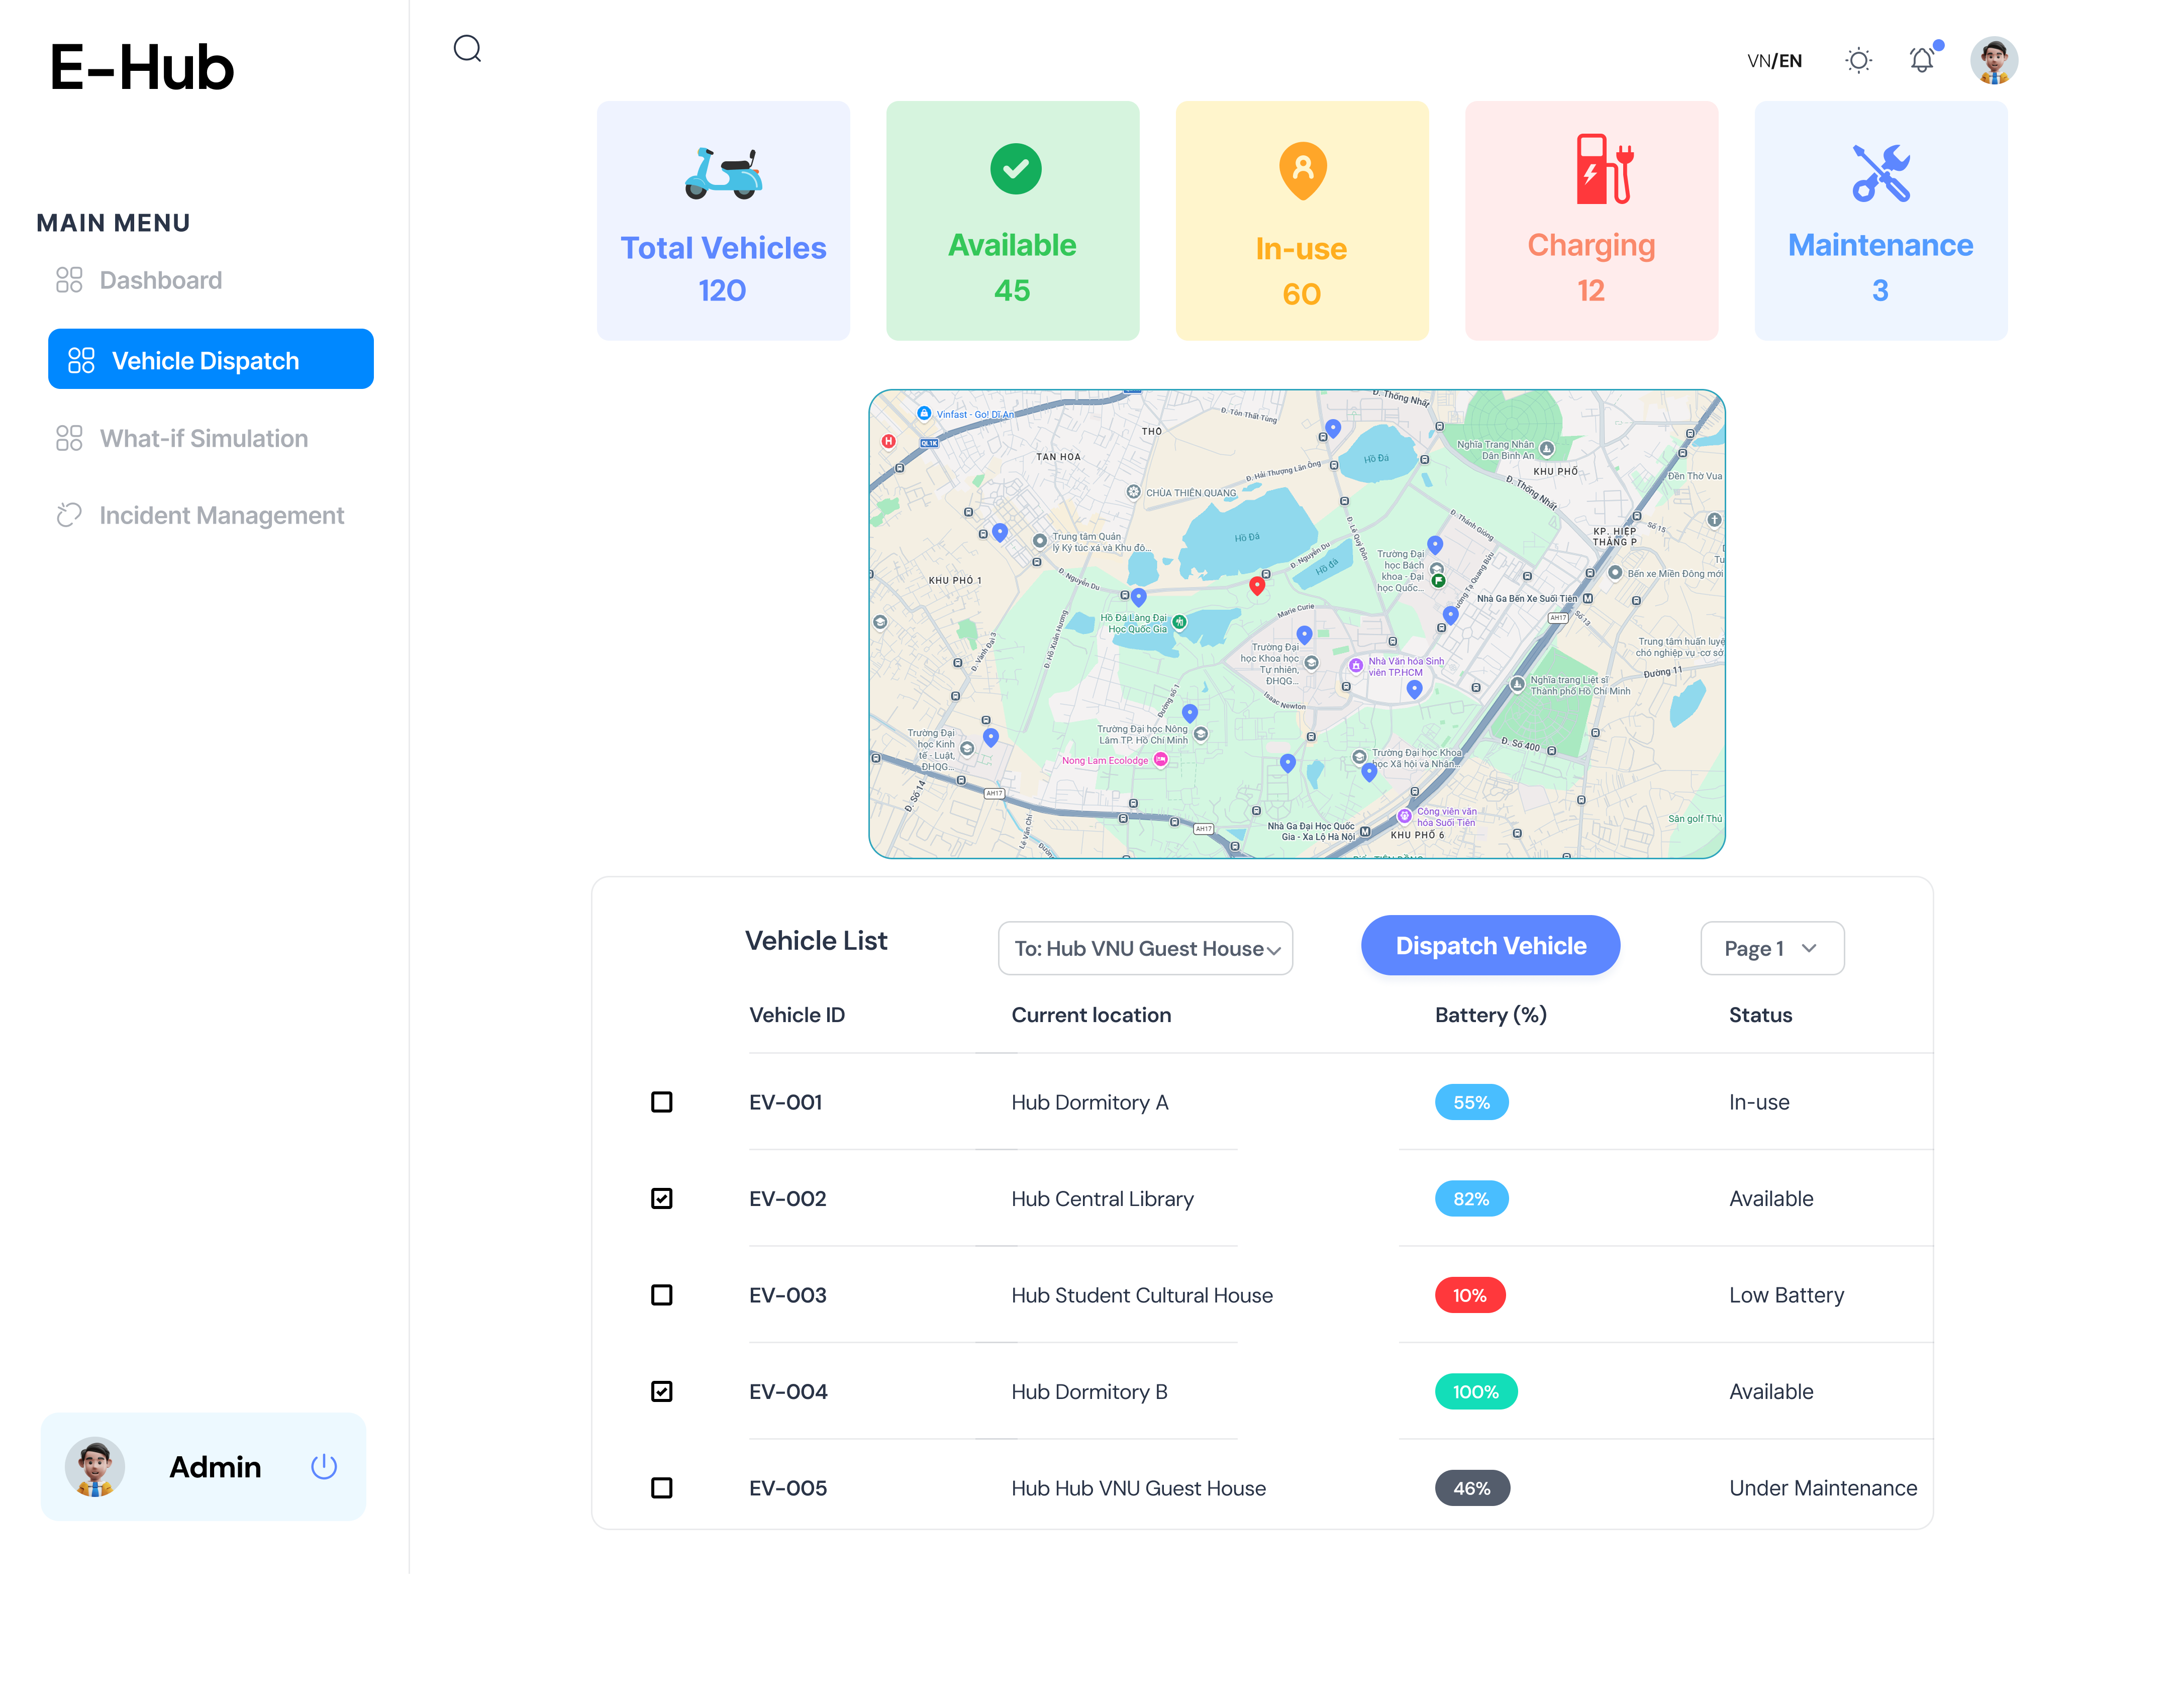
\includegraphics[width=0.96\linewidth,height=0.4\textheight,keepaspectratio]{s2/UI/DispatchScreen.png}
\captionof{figure}{Màn hình lập lệnh điều phối phương tiện giữa các Hub (UC11).}
\label{fig:dispatch_screen}
\par\vspace{0.5em}
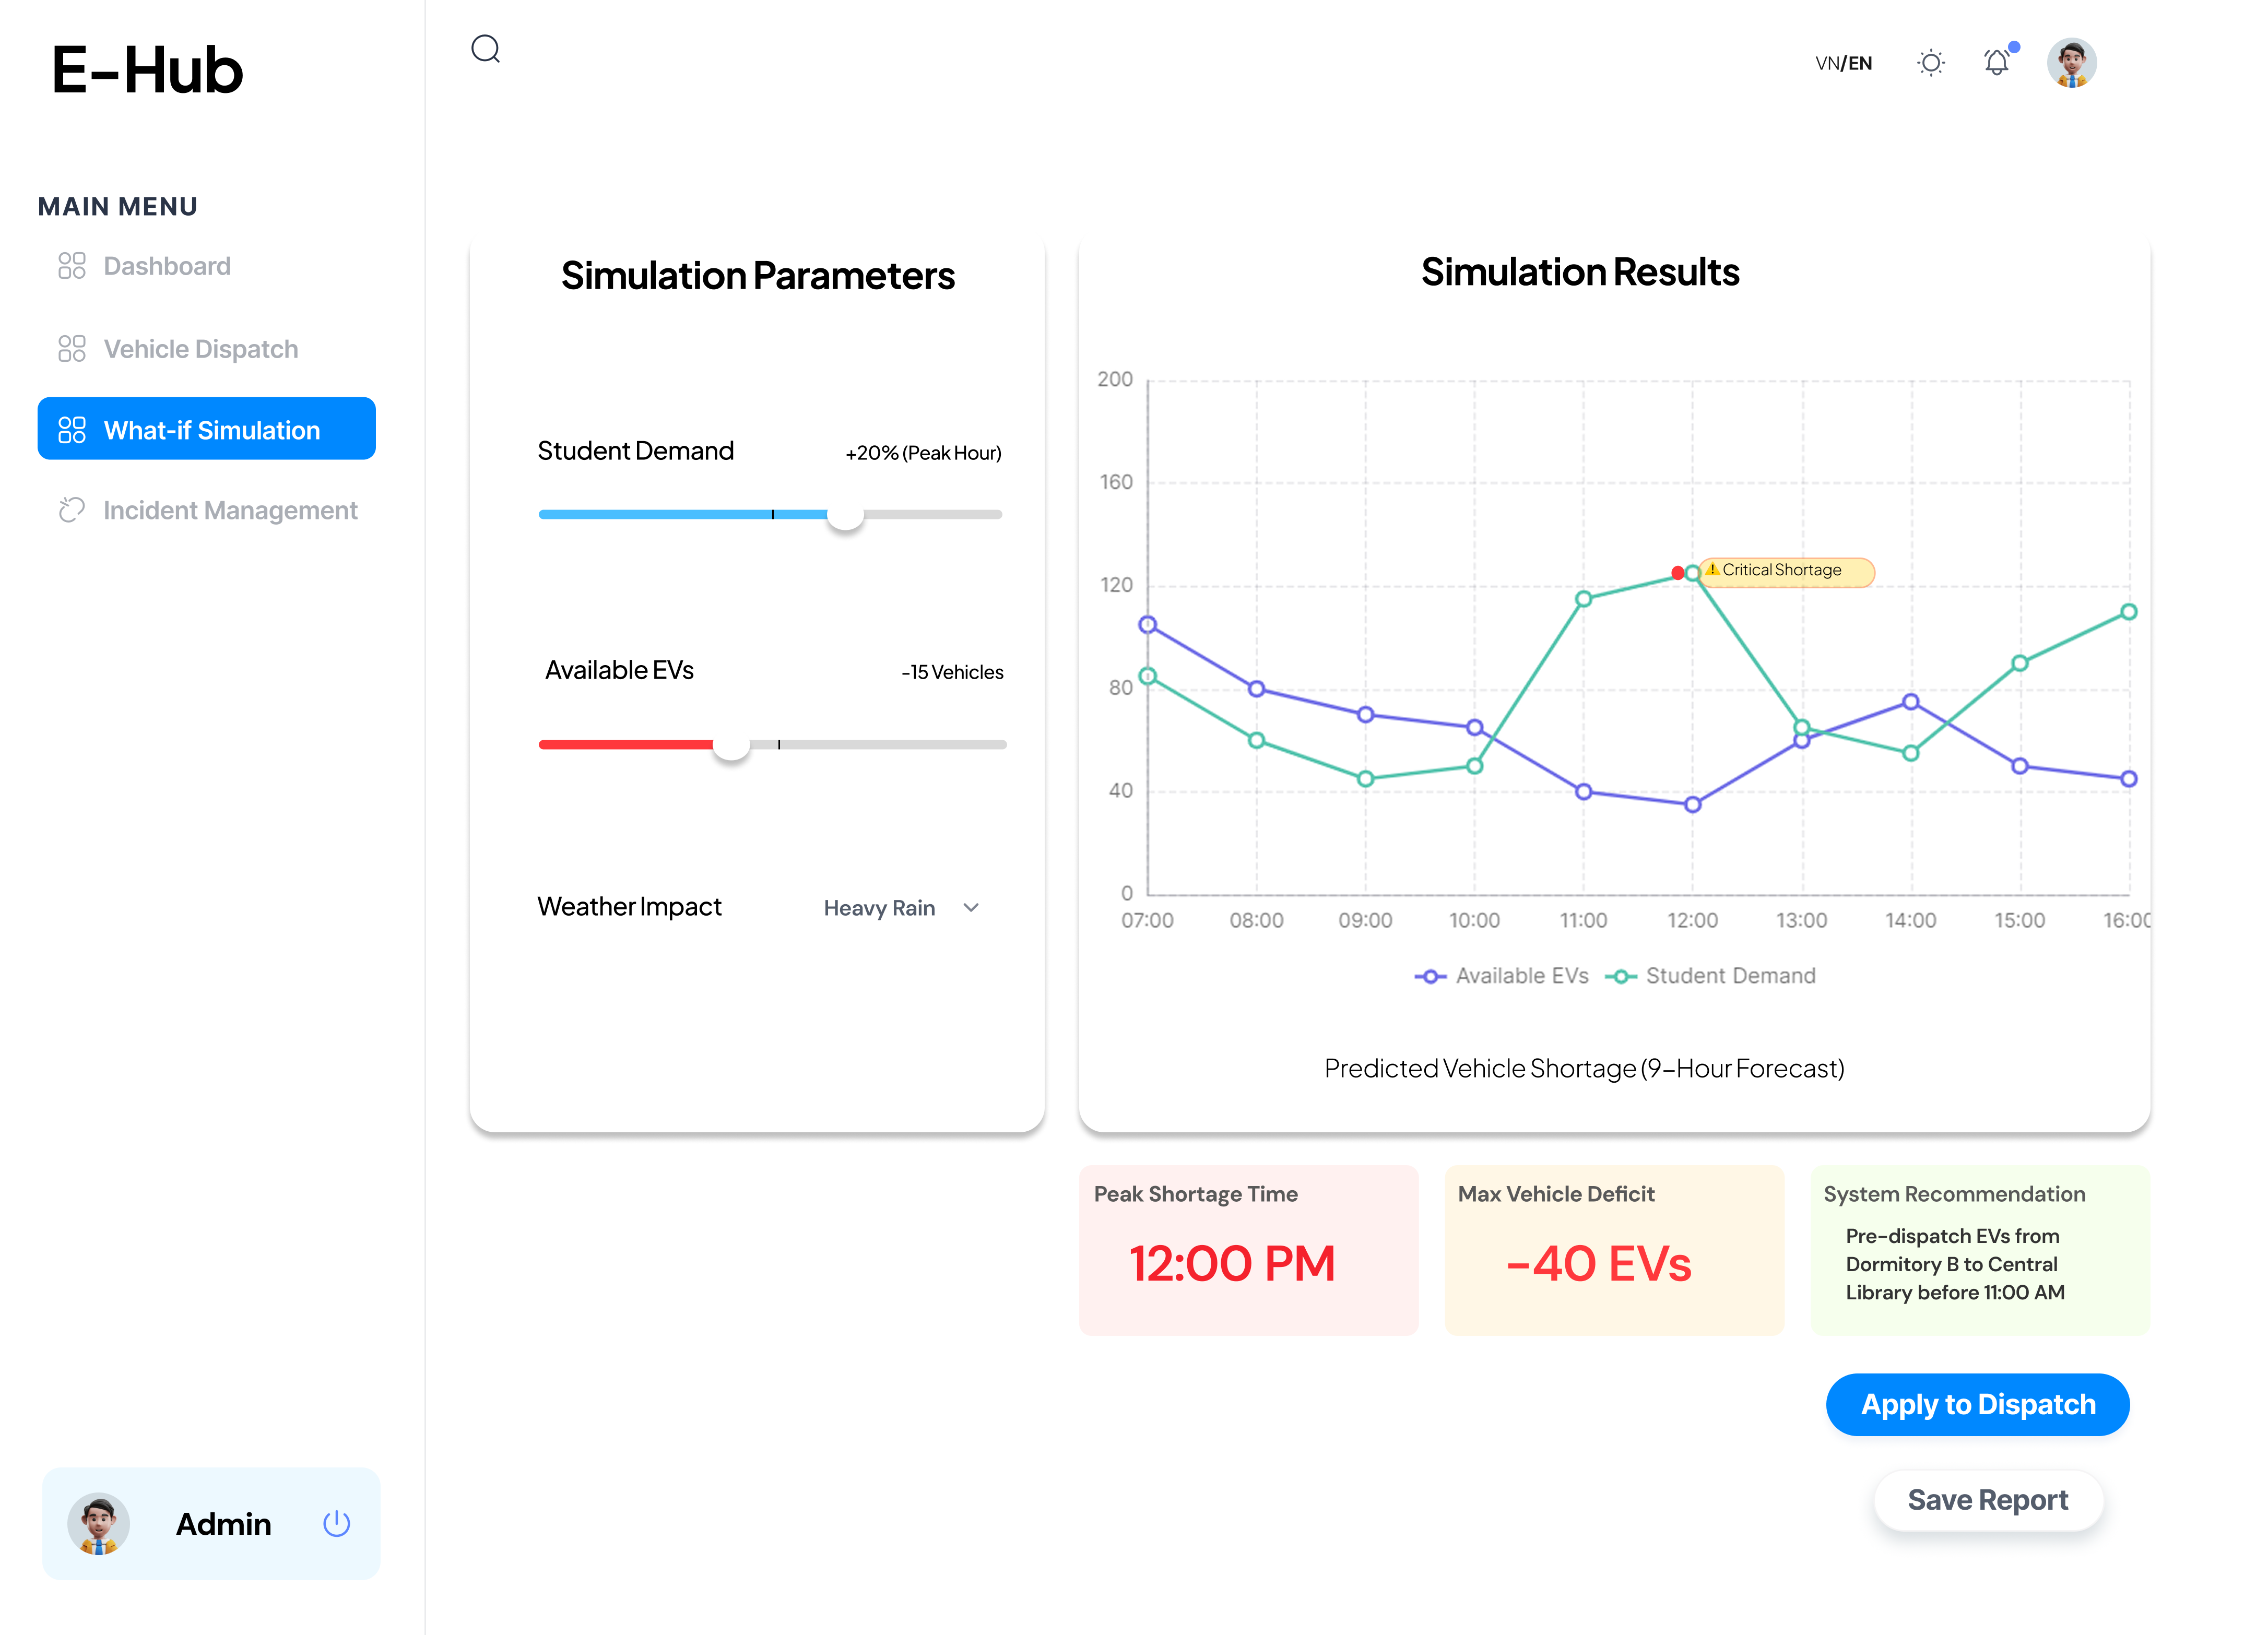
\includegraphics[width=0.96\linewidth,height=0.4\textheight,keepaspectratio]{s2/UI/SimulationPanel.png}
\captionof{figure}{Panel mô phỏng kịch bản What-if và dự báo nhu cầu (UC13, UC14).}
\label{fig:simulation_panel}
\end{figure}
\clearpage
\restoregeometry

\clearpage
\section{ACTIVITY DIAGRAM}

\insertsplitdiagram{ACTIVITY_DIAGRAM/AD1_1.drawio.png}{ACTIVITY_DIAGRAM/AD1_2.png}{Activity Diagram AD1 .}{fig:activity-ad1}
\insertdiagram{ACTIVITY_DIAGRAM/AD2.drawio.png}{Activity Diagram AD2.}{fig:activity-ad2}
\insertdiagram{ACTIVITY_DIAGRAM/AD3.drawio.png}{Activity Diagram AD3.}{fig:activity-ad3}
\insertdiagram{ACTIVITY_DIAGRAM/AD4.drawio.png}{Activity Diagram AD4.}{fig:activity-ad4}
\insertdiagram{ACTIVITY_DIAGRAM/AD5.png}{Activity Diagram AD5.}{fig:activity-ad5}
\insertdiagram{ACTIVITY_DIAGRAM/AD6.png}{Activity Diagram AD6.}{fig:activity-ad6}
\insertdiagram{ACTIVITY_DIAGRAM/AD7.png}{Activity Diagram AD7.}{fig:activity-ad7}
\insertdiagram{ACTIVITY_DIAGRAM/AD7E.png}{Activity Diagram AD7E -- UC7 AF3: Sạc khẩn cấp.}{fig:activity-ad7e}
\insertdiagram{ACTIVITY_DIAGRAM/AD8.png}{Activity Diagram AD8.}{fig:activity-ad8}
\insertdiagram{ACTIVITY_DIAGRAM/AD9.png}{Activity Diagram AD9.}{fig:activity-ad9}
\insertdiagram{ACTIVITY_DIAGRAM/AD10.png}{Activity Diagram AD10.}{fig:activity-ad10}
\insertdiagram{ACTIVITY_DIAGRAM/AD11.drawio.png}{Activity Diagram AD11.}{fig:activity-ad11}
\insertdiagram{ACTIVITY_DIAGRAM/AD12.png}{Activity Diagram AD12.}{fig:activity-ad12}
\insertdiagram{ACTIVITY_DIAGRAM/AD13.drawio.png}{Activity Diagram AD13.}{fig:activity-ad13}
\insertdiagram{ACTIVITY_DIAGRAM/AD14.drawio.png}{Activity Diagram AD14.}{fig:activity-ad14}
\insertdiagram{ACTIVITY_DIAGRAM/AD15.png}{Activity Diagram AD15.}{fig:activity-ad15}
\insertdiagram{ACTIVITY_DIAGRAM/AD16.png}{Activity Diagram AD16.}{fig:activity-ad16}
\insertdiagram{ACTIVITY_DIAGRAM/AD17.png}{Activity Diagram AD17.}{fig:activity-ad17}

\clearpage
\section{SEQUENCE DIAGRAM}

\insertsplitdiagram{SEQUENCE_DIAGRAM/SD1_1.png}{SEQUENCE_DIAGRAM/SD1_2.png}{Sequence Diagram SD1 .}{fig:sequence-sd1}
\insertdiagram{SEQUENCE_DIAGRAM/SD2.drawio.png}{Sequence Diagram SD2.}{fig:sequence-sd2}
\insertdiagram{SEQUENCE_DIAGRAM/SD3.drawio.png}{Sequence Diagram SD3.}{fig:sequence-sd3}
\insertdiagram{SEQUENCE_DIAGRAM/SD4.drawio.png}{Sequence Diagram SD4.}{fig:sequence-sd4}
\insertdiagram{SEQUENCE_DIAGRAM/SD5.png}{Sequence Diagram SD5.}{fig:sequence-sd5}
\insertsplitdiagram{SEQUENCE_DIAGRAM/SD06_Pic1.png}{SEQUENCE_DIAGRAM/SD06_Pic2.png}{Sequence Diagram SD6 .}{fig:sequence-sd6}
\insertsplitdiagram{SEQUENCE_DIAGRAM/SD07_Pic1.png}{SEQUENCE_DIAGRAM/SD07_Pic2.png}{Sequence Diagram SD7 .}{fig:sequence-sd7}
\insertdiagram{SEQUENCE_DIAGRAM/SD07E_SacKhanCap.png}{Sequence Diagram SD7E -- UC7 AF3: Sạc khẩn cấp.}{fig:sequence-sd7e}
\insertdiagram{SEQUENCE_DIAGRAM/SD8.drawio.png}{Sequence Diagram SD8.}{fig:sequence-sd8}
\insertdiagram{SEQUENCE_DIAGRAM/SD9.drawio.png}{Sequence Diagram SD9.}{fig:sequence-sd9}
\insertdiagram{SEQUENCE_DIAGRAM/SD10.drawio.png}{Sequence Diagram SD10.}{fig:sequence-sd10}
\insertdiagram{SEQUENCE_DIAGRAM/SD11.drawio.png}{Sequence Diagram SD11.}{fig:sequence-sd11}
\insertdiagram{SEQUENCE_DIAGRAM/SD12.drawio.png}{Sequence Diagram SD12.}{fig:sequence-sd12}
\insertdiagram{SEQUENCE_DIAGRAM/SD13.drawio.png}{Sequence Diagram SD13.}{fig:sequence-sd13}
\insertdiagram{SEQUENCE_DIAGRAM/SD14.drawio.png}{Sequence Diagram SD14.}{fig:sequence-sd14}
\insertdiagram{SEQUENCE_DIAGRAM/SD15.png}{Sequence Diagram SD15.}{fig:sequence-sd15}
\insertdiagram{SEQUENCE_DIAGRAM/SD16.png}{Sequence Diagram SD16.}{fig:sequence-sd16}
\insertsplitdiagram{SEQUENCE_DIAGRAM/SD17_Pic1.png}{SEQUENCE_DIAGRAM/SD17_Pic2.png}{Sequence Diagram SD17 .}{fig:sequence-sd17}

\clearpage
\section{STATE CHART}

\insertdiagram{cho_do_xe_state-chart.drawio.png}{State chart chỗ đỗ xe}{fig:state-chart-cho-do-xe}
\insertdiagram{cong_sac_state-chart.drawio.png}{State chart cổng sạc}{fig:state-chart-cong-sac}
\insertdiagram{xe_dien_state-chart.drawio.png}{State chart xe điện}{fig:state-chart-xe-dien}

\endgroup
\newpage

%%%%%%%%%%%%%%%%% SUBMISSION 3 %%%%%%%%%%%%%%%%%%%
\part{Kiến trúc, Thiết kế chi tiết và Kiểm thử (Submission 3)}
\section{Các diagram trong bài tập lớn}
\subsection{Class diagram tổng quát}
\begin{figure}[H]
\centering
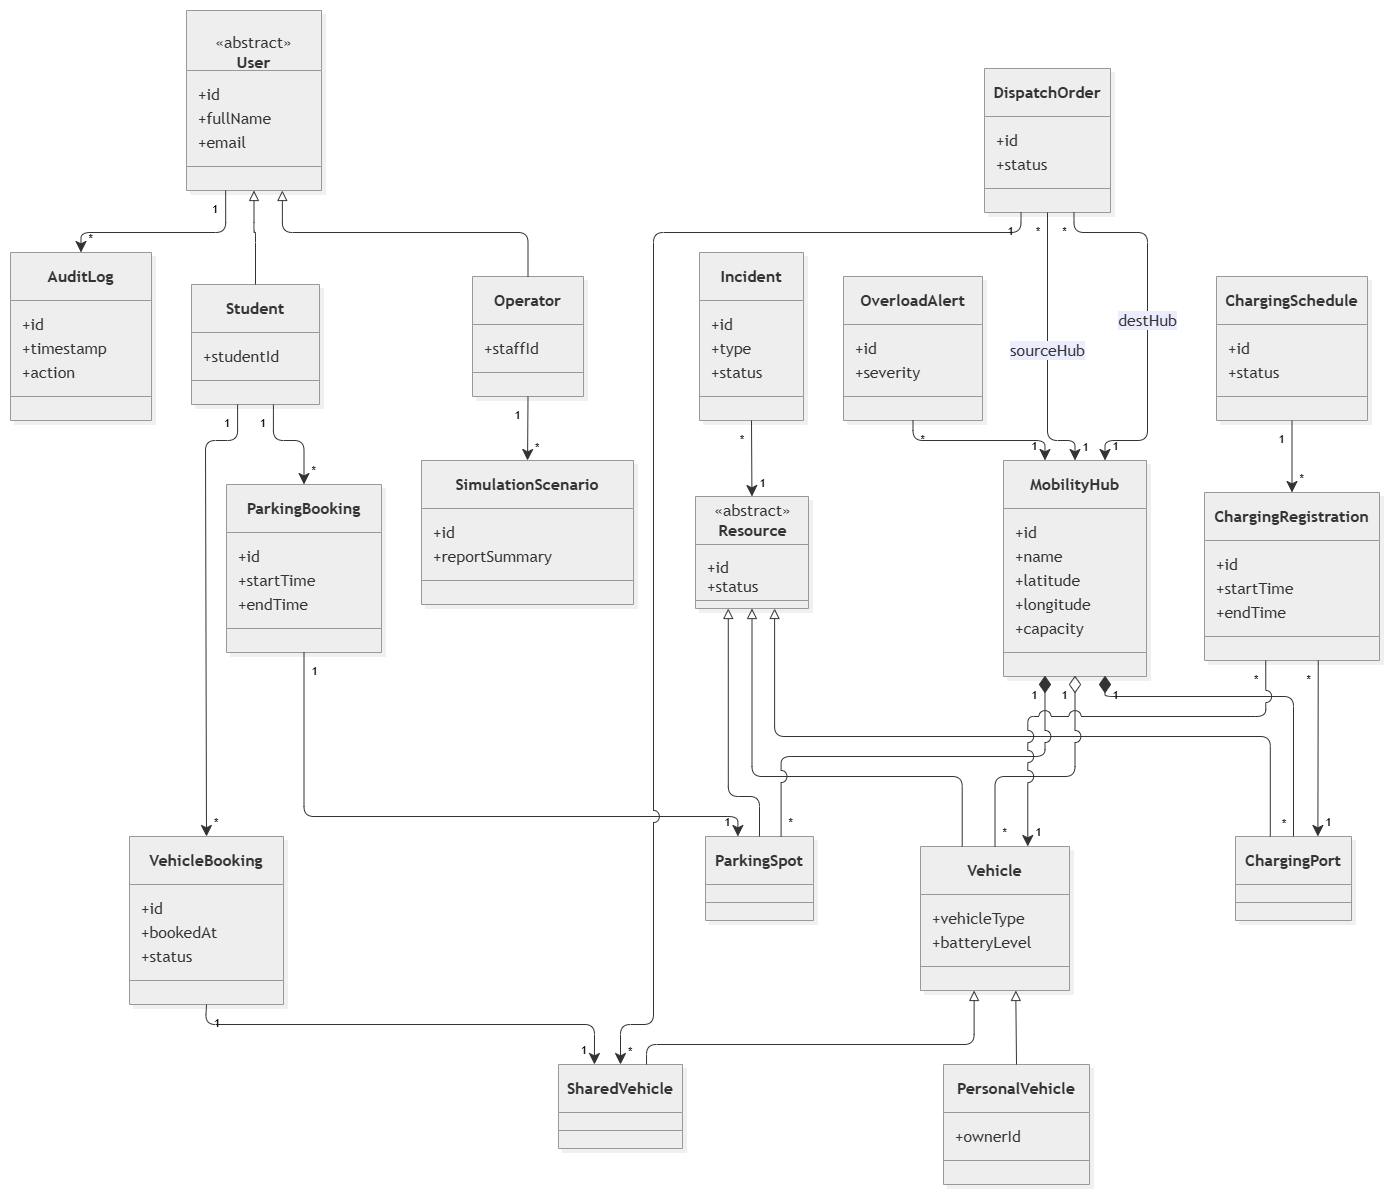
\includegraphics[width=\textwidth,height=0.82\textheight,keepaspectratio]{s3/class_diagram_submission3.drawio.png}
\end{figure}
\clearpage

\subsection{Deployment view}
\begin{figure}[H]
\centering
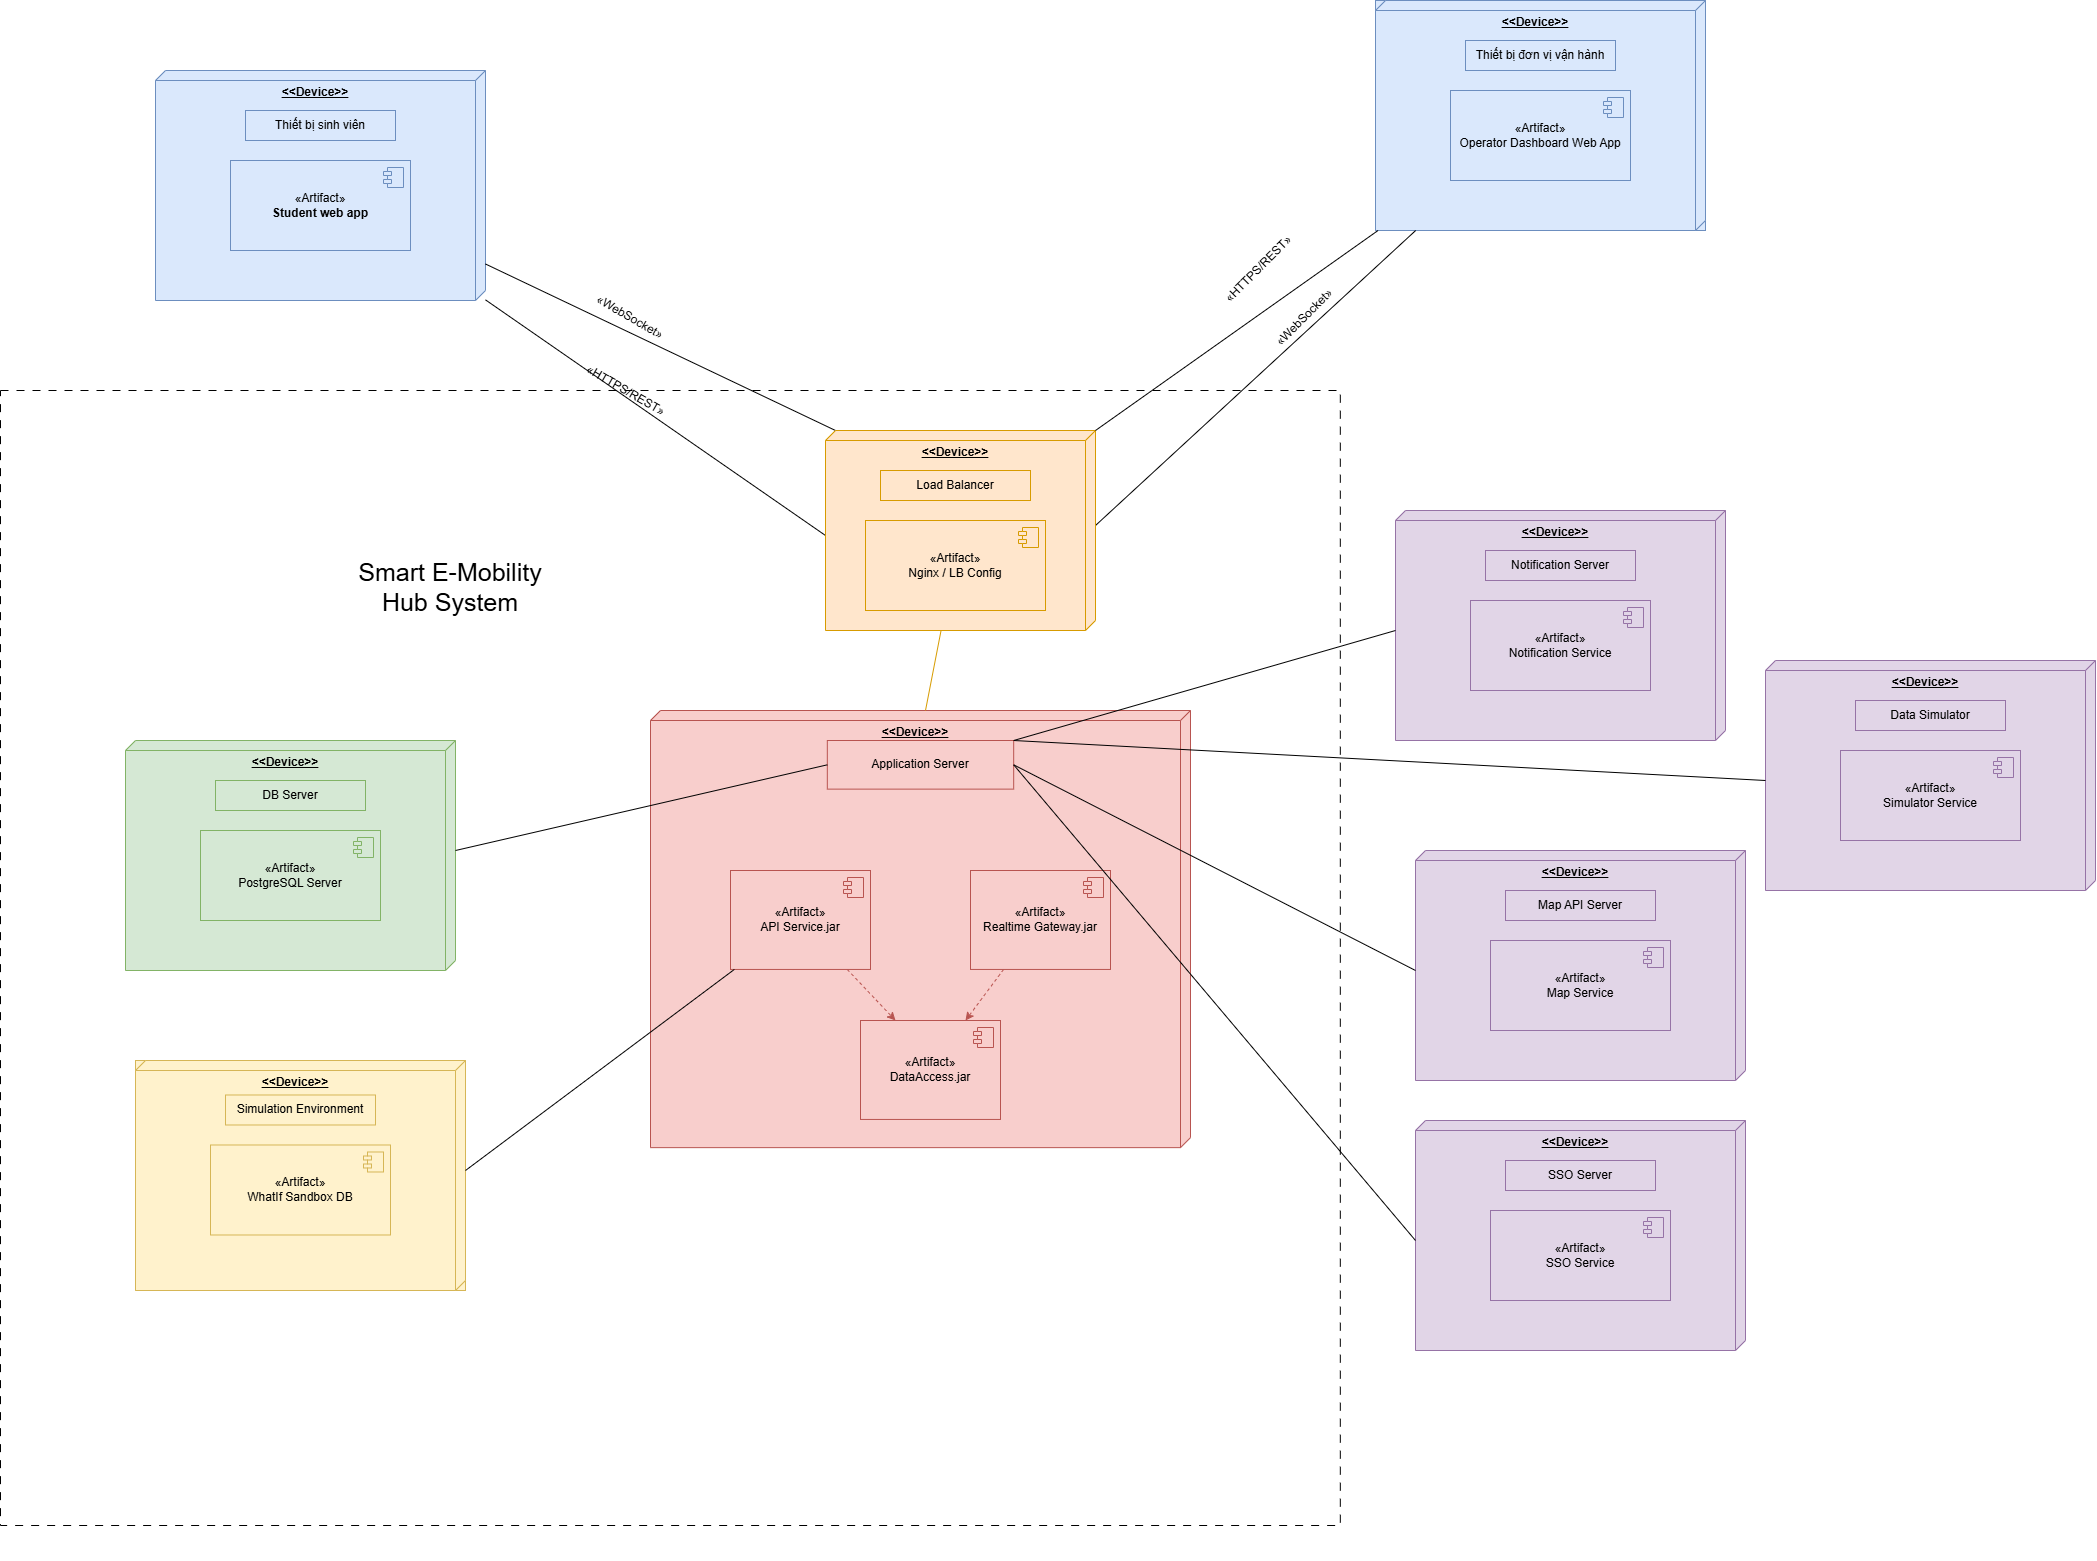
\includegraphics[width=\textwidth,height=0.82\textheight,keepaspectratio]{s3/deployment_view.drawio.png}
\end{figure}
\clearpage

\subsection{Implementation view}
\begin{figure}[H]
\centering
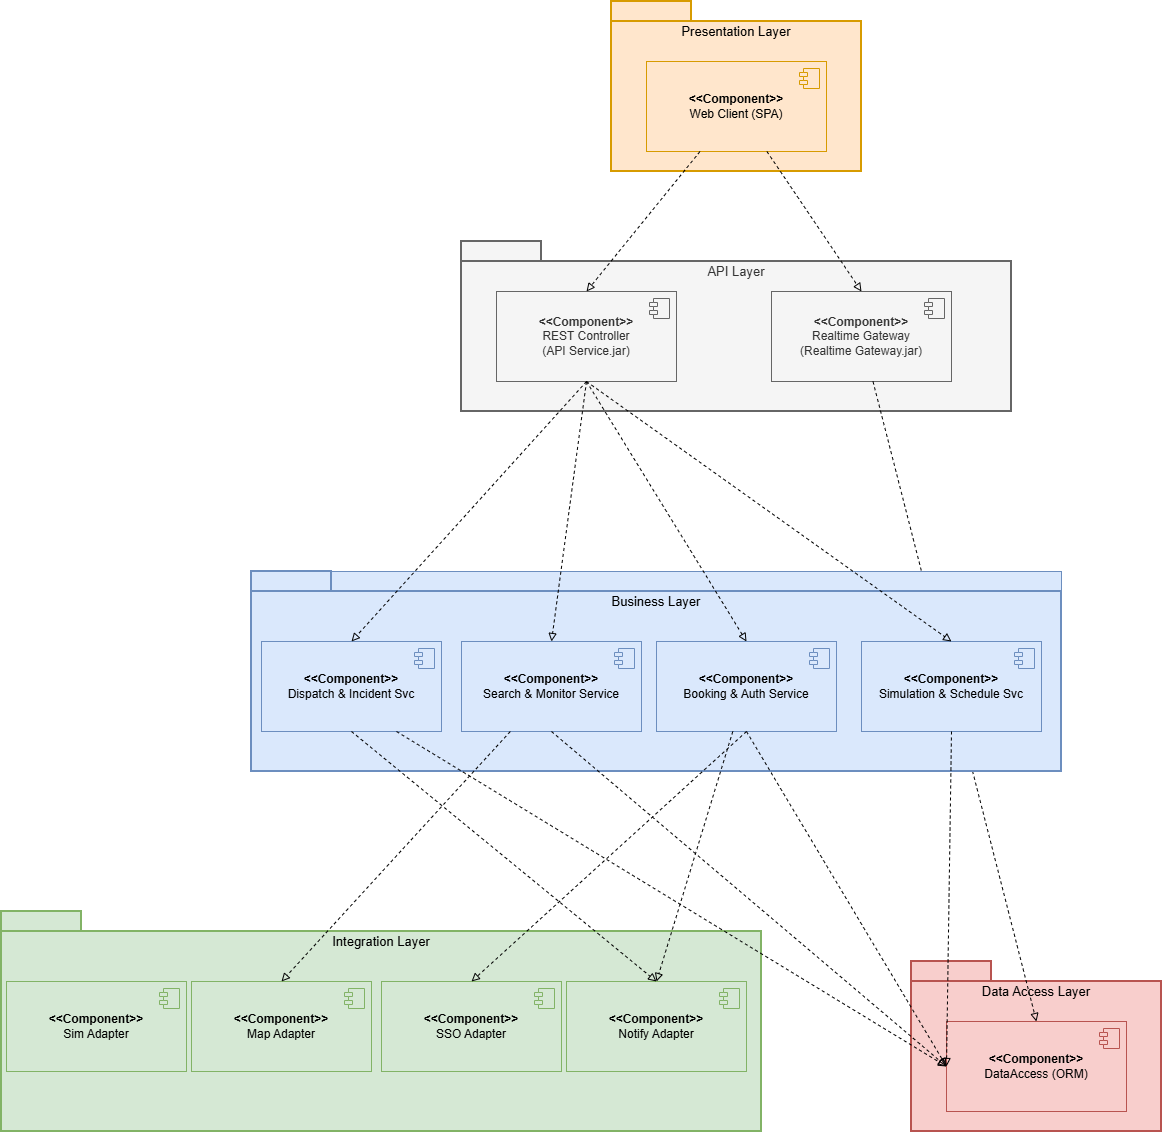
\includegraphics[width=\textwidth,height=0.82\textheight,keepaspectratio]{s3/implementation_view.drawio.png}
\end{figure}
\clearpage

\subsection{Class diagram UC1, UC2, UC8}
\begin{figure}[H]
\centering
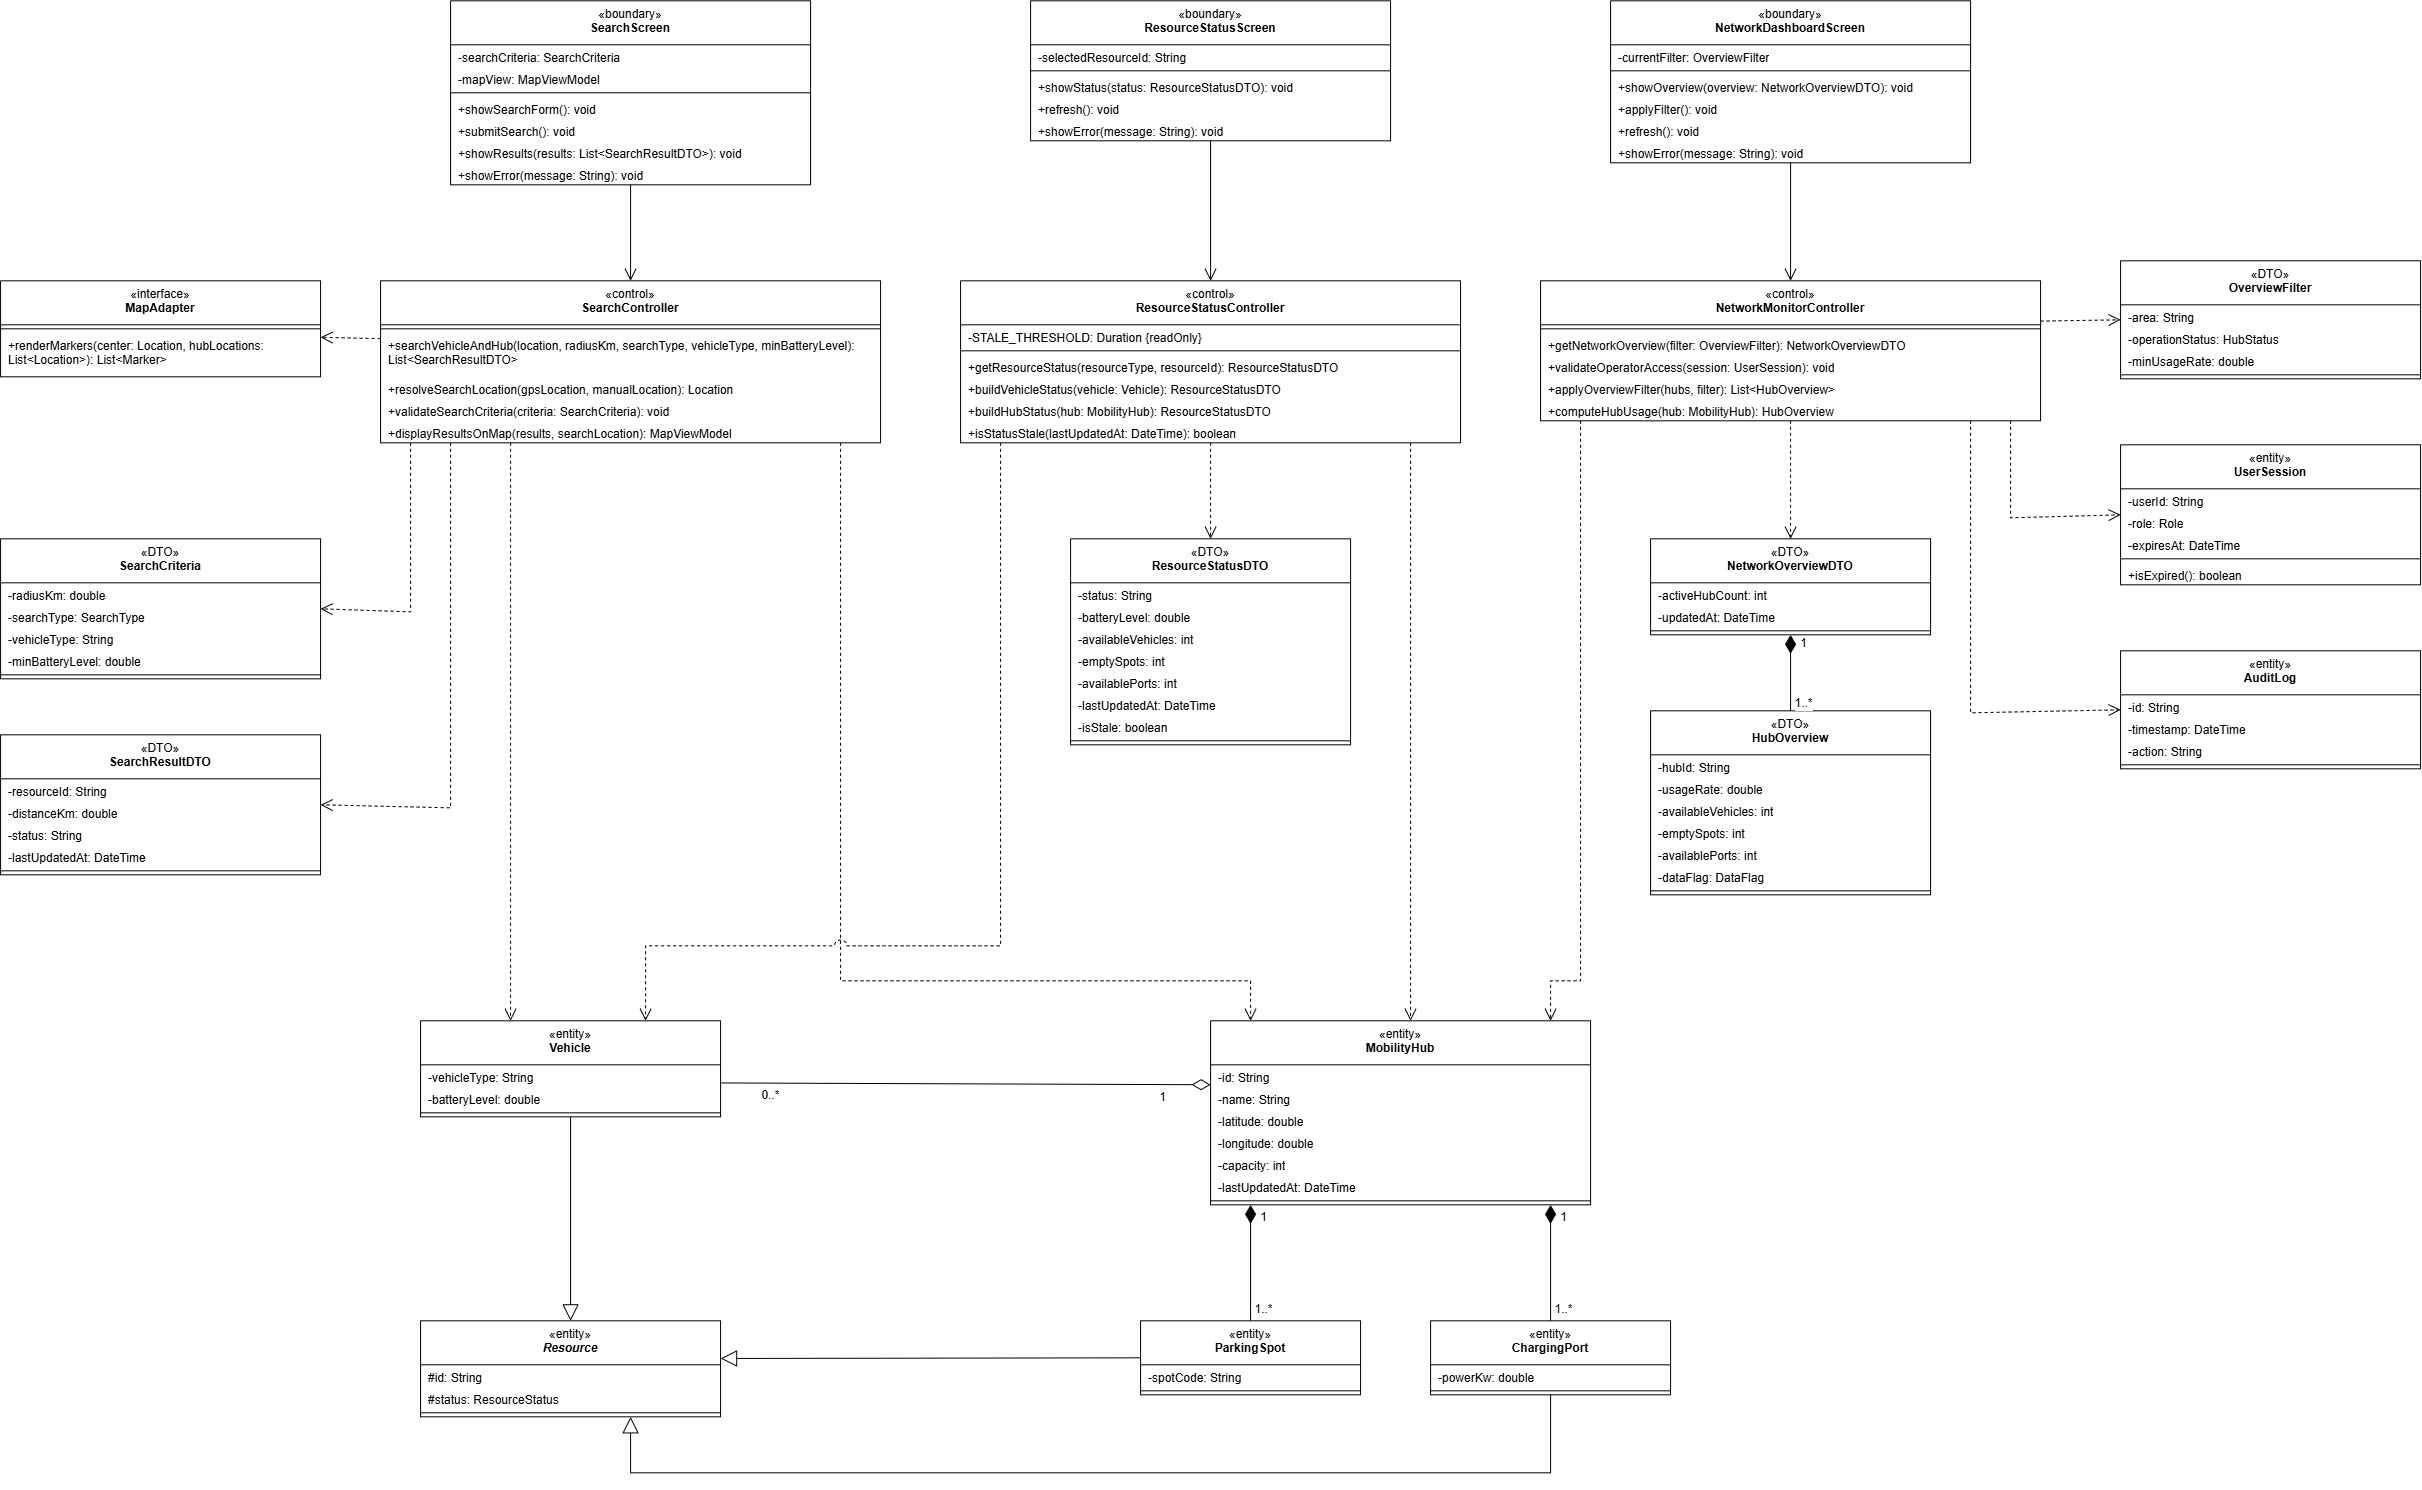
\includegraphics[width=\textwidth,height=0.82\textheight,keepaspectratio]{s3/ClassDiagram_UC1_UC2_UC8.png}
\end{figure}
\clearpage

\subsection{Class diagram UC3, UC4, UC5, UC17}
\begin{figure}[H]
\centering
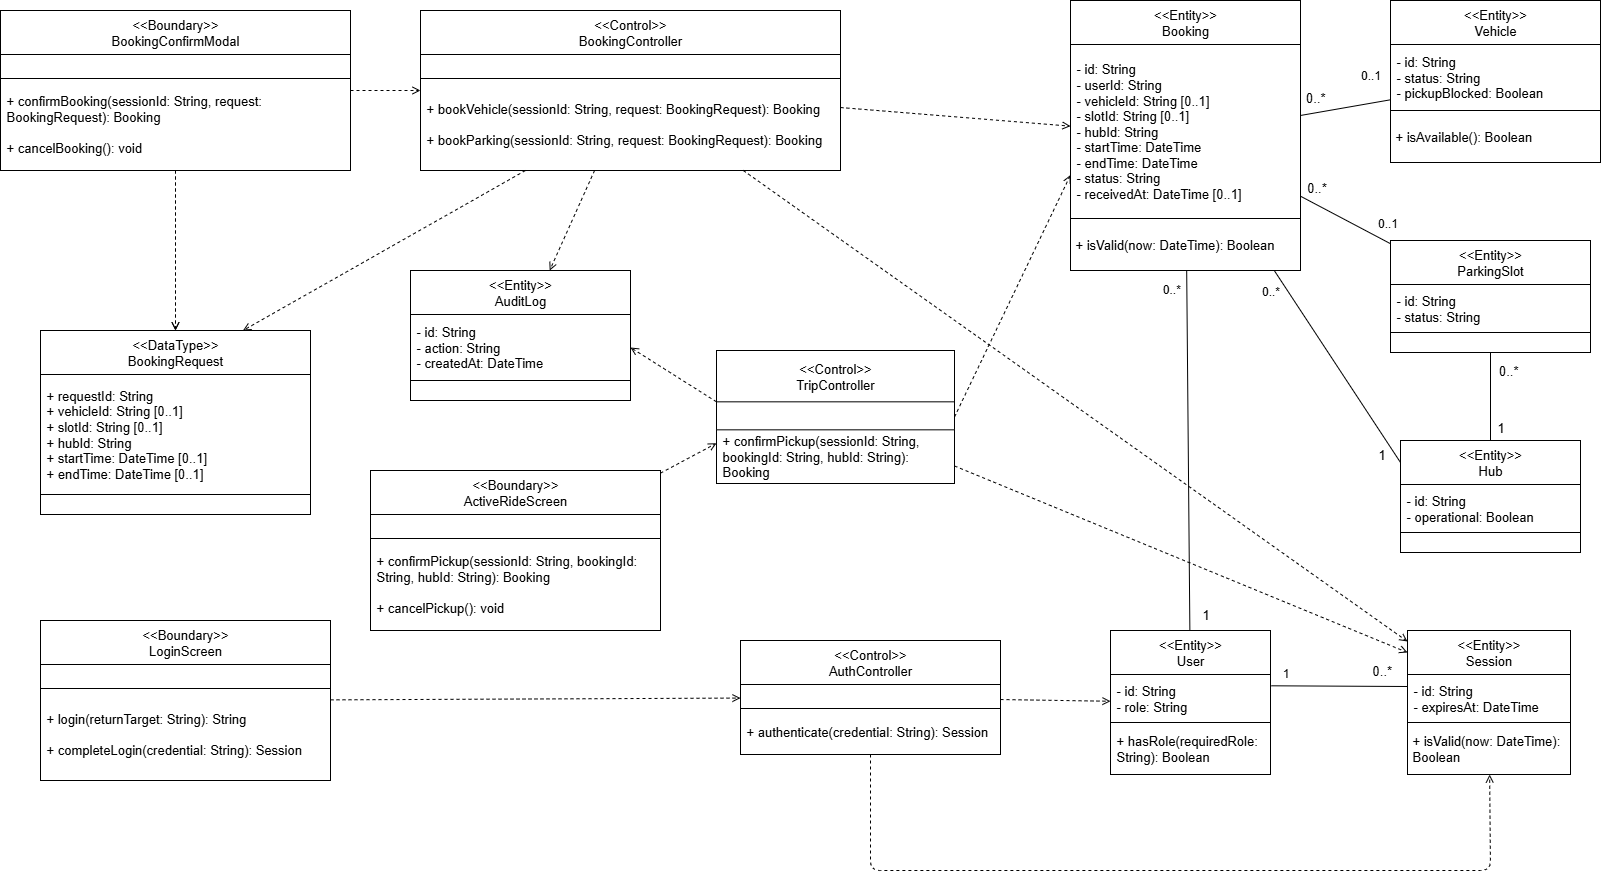
\includegraphics[width=\textwidth,height=0.82\textheight,keepaspectratio]{s3/Class_diagram_UC_3_4_5_17.png}
\end{figure}
\clearpage

\subsection{Class diagram UC6, UC7, UC9, UC10}
\begin{figure}[H]
\centering
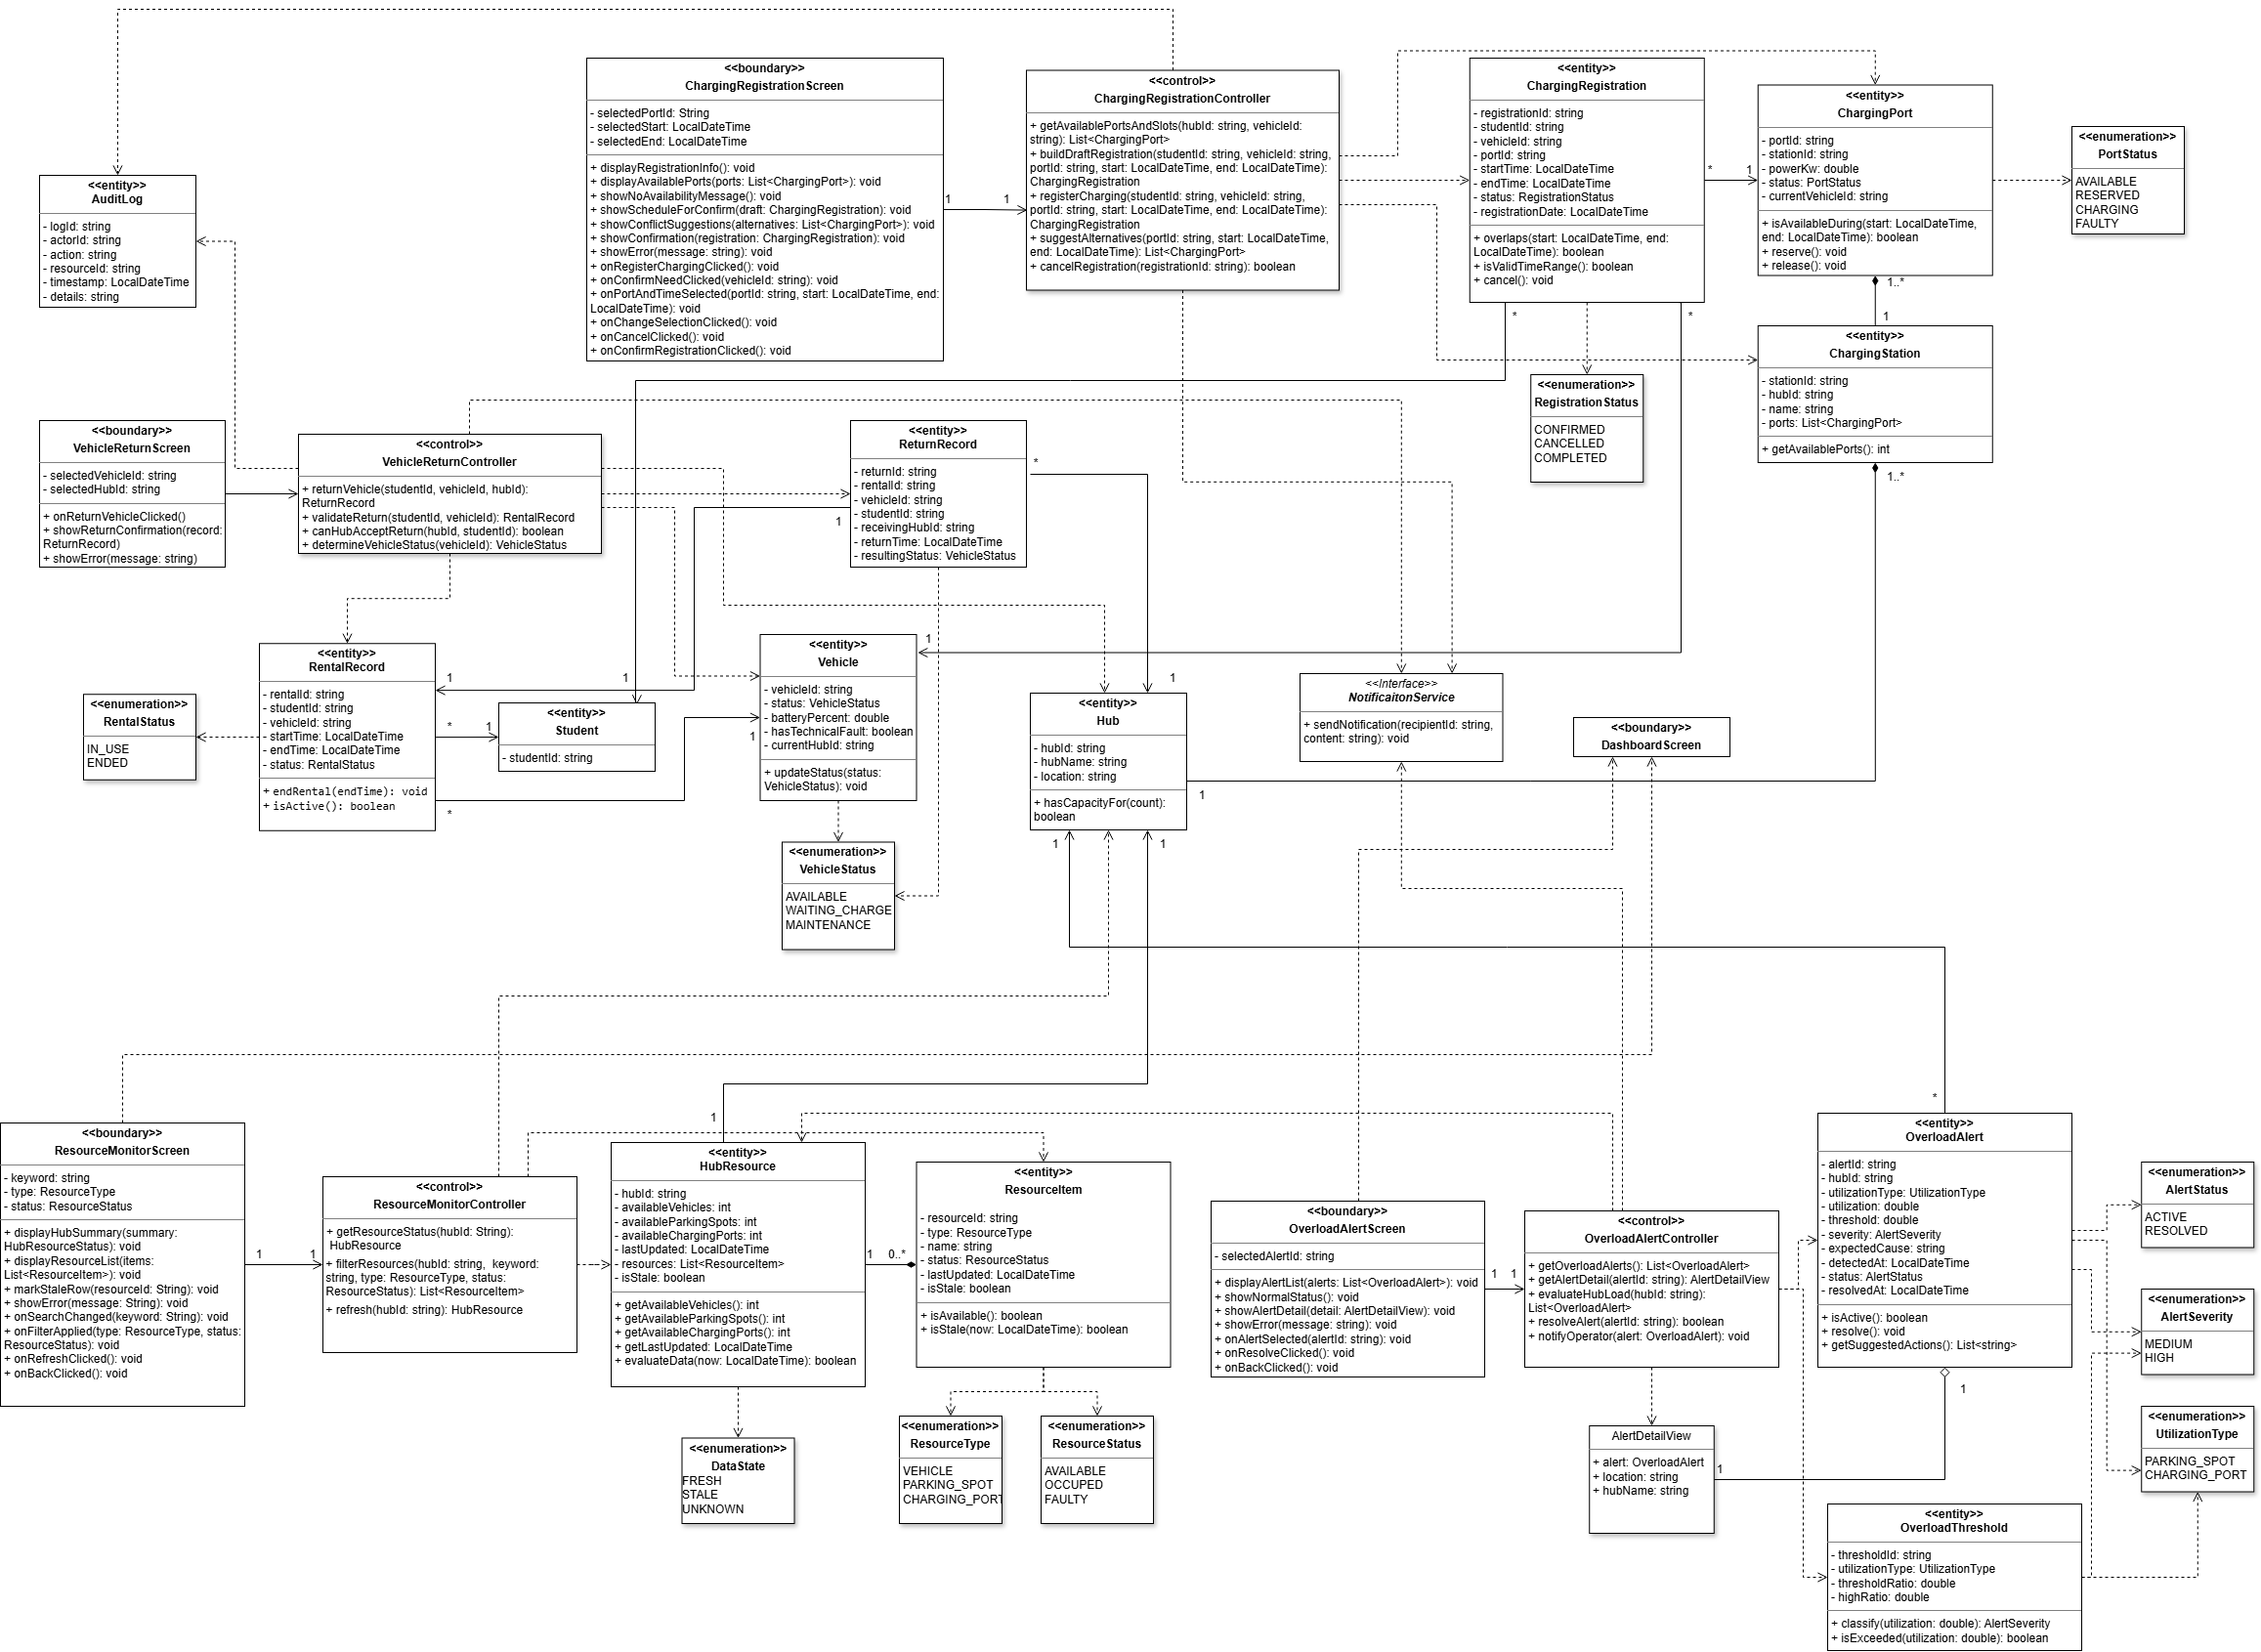
\includegraphics[width=\textwidth,height=0.82\textheight,keepaspectratio]{s3/Class_diagram_UC_6_7_9_10.png}
\end{figure}
\clearpage

\subsection{Class diagram UC11, UC12, UC16}
\begin{figure}[H]
\centering
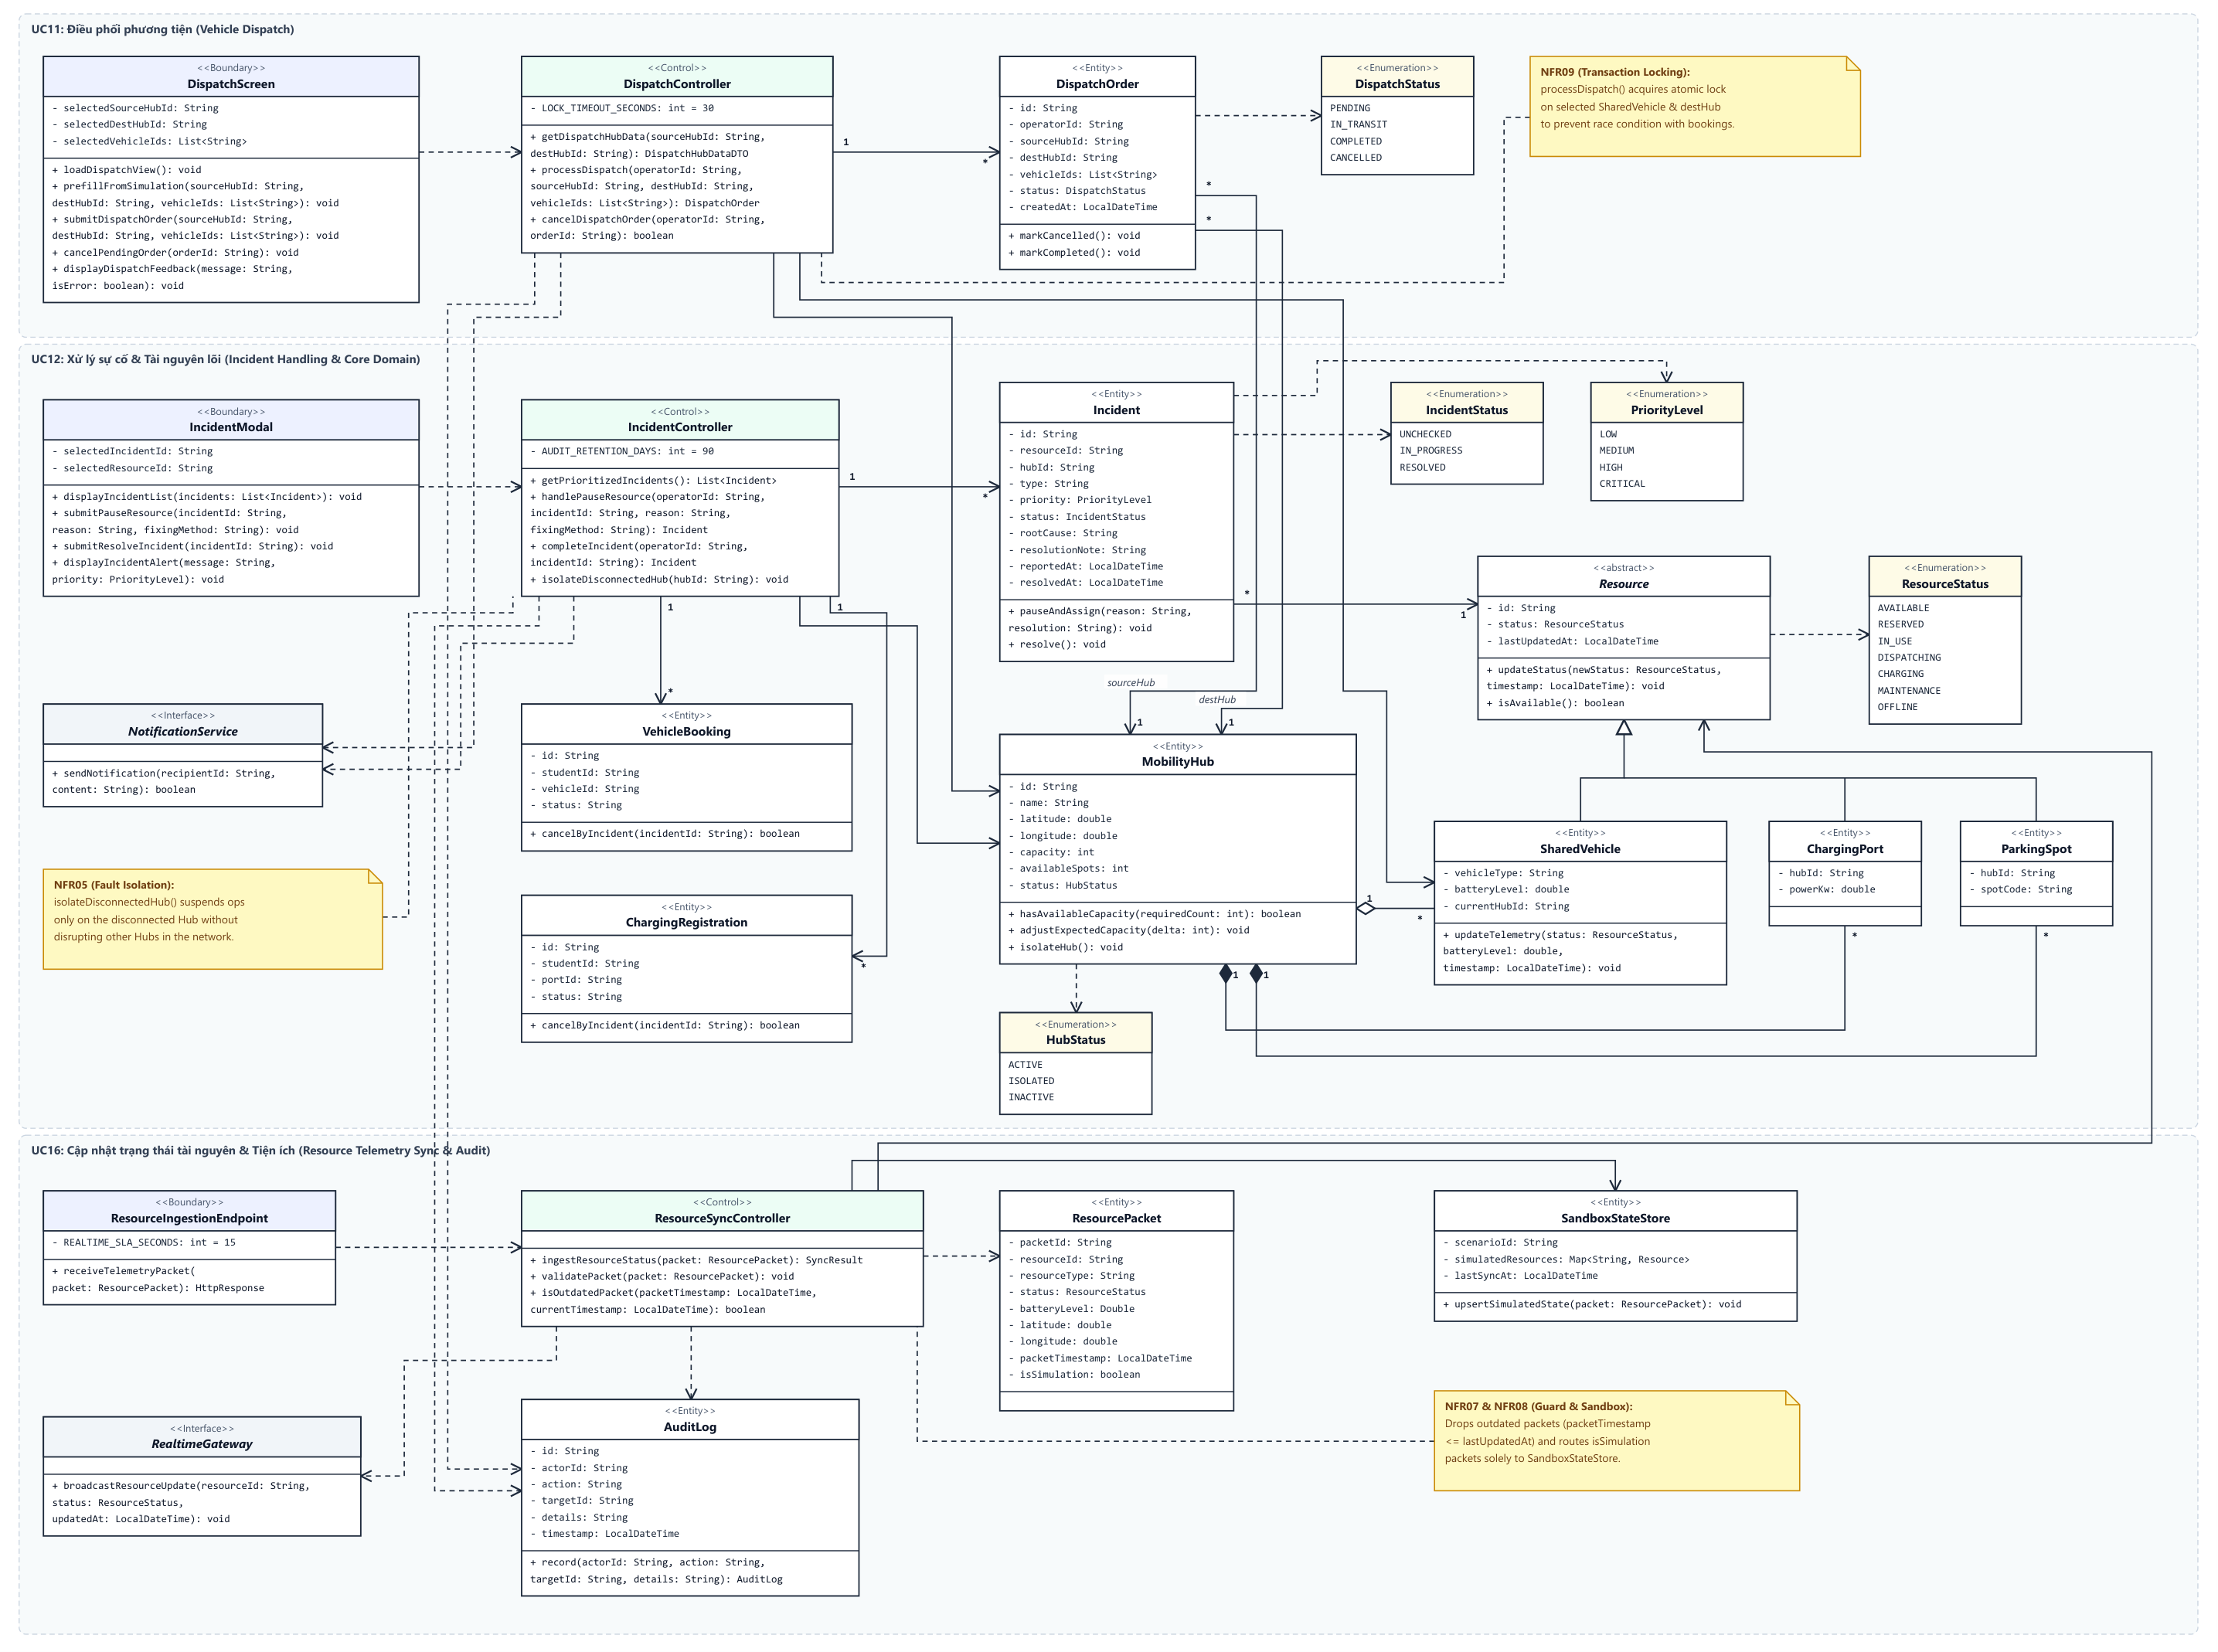
\includegraphics[width=\textwidth,height=0.82\textheight,keepaspectratio]{s3/Class_diagram_UC_11_12_16.png}
\end{figure}
\clearpage

\subsection{Class diagram UC12, UC13, UC14, UC15}
\begin{figure}[H]
\centering
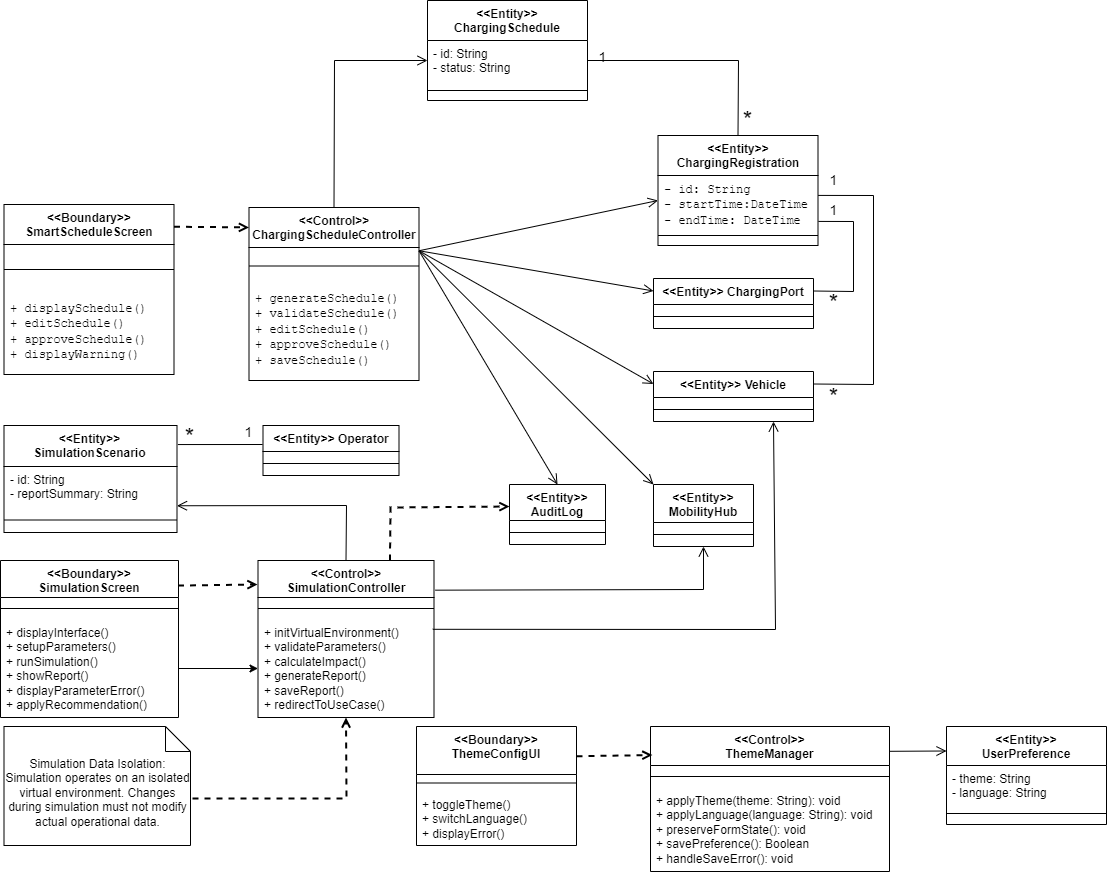
\includegraphics[width=\textwidth,height=0.82\textheight,keepaspectratio]{s3/Class_diagram_UC_13_14_15.png}
\end{figure}
\clearpage
\newpage
\small
\renewcommand{\arraystretch}{1.12}
\section{Đặc tả phương thức (Methods Description)}
\subsection{Use Case UC1 - Tìm phương tiện và Hub phù hợp}
\subsubsection{searchVehicleAndHub()}
\begin{longtable}{|L{0.24\textwidth}|L{0.70\textwidth}|}
\hline
\textbf{Thuộc tính} & \textbf{Nội dung chi tiết} \\
\hline
\endfirsthead
\hline
\textbf{Thuộc tính} & \textbf{Nội dung chi tiết} \\
\hline
\endhead
\textbf{Tên phương thức} & searchVehicleAndHub() \\
\hline
\textbf{Mục đích} & Tìm các phương tiện điện dùng chung hoặc Mobility Hub phù hợp\newline với vị trí và tiêu chí tìm kiếm của sinh viên, hỗ trợ cả 2 kiểu tìm\newline (theophươngtiện - Normal Flow, hoặc theo Hub - AF2). \\
\hline
\textbf{Tham số đầu vào}\newline \textbf{(@param)} & location: Location - vị trí tìm kiếm (GPS hoặc chọn thủ công, AF1);\newline radiusKm: double - bán kính tìm; searchType: SearchType\newline \{VEHICLE, HUB\}; vehicleType: String - loại xe mong muốn (chỉ\newline áp dụng khi searchType=VEHICLE); minBatteryLevel: double -\newline mứcpin tối thiểu(chỉ ápdụngkhi searchType=VEHICLE). \\
\hline
\textbf{Giá trị trả về (@return)} & List<SearchResultDTO> - danh sách kết quả sắp xếp theo khoảng\newline cách tăng dần, kèm trạng thái và thời điểm cập nhật; danh sách rỗng\newline nếu khôngcó kếtquảphù hợp (AF3). \\
\hline
\textbf{Ngoại lệ (@exception)} & InvalidLocationException (EX1); InvalidSearchCriteriaException\newline (EX2); MapServiceUnavailableException (EX3);\newline DataSourceUnavailableException(EX4). \\
\hline
\textbf{Tiền điều kiện (Pre-}\newline \textbf{conditions)} & Hệ thống đã cấu hình danh mục và toạ độ các Hub thuộc phạm vi\newline phục vụ; khôngbắt buộc sinh viên đăngnhập. \\
\hline
\textbf{Hậu điều kiện (Post-}\newline \textbf{conditions)} & Trả về kết quả phù hợp kèm thời điểm cập nhật, hoặc danh sách\newline rỗng; không ghi/sửa bất kỳdữ liệu nào(thao tác chỉ đọc). \\
\hline
 & function searchVehicleAndHub(location, radiusKm, searchType,\newline vehicleType, minBatteryLevel):\newline if location == null: throw InvalidLocationException\newline if radiusKm <= 0: throw InvalidSearchCriteriaException\newline try:\newline candidates = dataAccess.findWithinRadius(\newline location, radiusKm, searchType)\newline catch DataAccessError: \\
\hline
\textbf{Luồng thuật toán}\newline \textbf{(Pseudo-code)} & throw DataSourceUnavailableException\newline if searchType == VEHICLE:\newline results = filter(candidates,\newline type==vehicleType AND battery>=minBatteryLevel\newline AND status==AVAILABLE)\newline else:\newline results = candidates\newline // kèm số xe/chỗ đỗ/cổng sạc khả dụng mỗi Hub\newline sort results by distance(location) ascending\newline return results \\
\hline
\end{longtable}
\vspace{-0.5\baselineskip}
\subsubsection{resolveSearchLocation()}
\begin{longtable}{|L{0.24\textwidth}|L{0.70\textwidth}|}
\hline
\textbf{Thuộc tính} & \textbf{Nội dung chi tiết} \\
\hline
\endfirsthead
\hline
\textbf{Thuộc tính} & \textbf{Nội dung chi tiết} \\
\hline
\endhead
\textbf{Tên phương thức} & resolveSearchLocation() \\
\hline
\textbf{Mục đích} & Xác định vị trí dùng làm tâm tìm kiếm: ưu tiên vị trí do Sinh viên\newline chọn thủ công trên bản đồ (AF1), nếu không có thì dùng toạ độ GPS\newline của thiết bị(bước 3-4 của UC1). \\
\hline
\textbf{Tham số đầu vào}\newline \textbf{(@param)} & gpsLocation: Location (nullable) - toạ độ GPS lấy từ thiết bị;\newline manualLocation: Location (nullable) - vị trí, khu vực hoặc Hub Sinh\newline viên chọn trên bản đồ. \\
\hline
\textbf{Giá trị trả về (@return)} & Location - vị trí tìm kiếm hợp lệ, nằm trong phạm vi phục vụ của\newline khu đô thị ĐHQG-HCM. \\
\hline
\textbf{Ngoại lệ (@exception)} & InvalidLocationException (EX1) - khi cả 2 tham số đều null hoặc vị\newline trí nằm ngoàiphạm viphục vụ. \\
\hline
\textbf{Tiền điều kiện (Pre-}\newline \textbf{conditions)} & Giao diện tìm kiếm đang hiển thị; phạm vi phục vụ\newline (SERVICE\_AREA)đã được cấu hình. \\
\hline
\textbf{Hậu điều kiện (Post-}\newline \textbf{conditions)} & Trả về đúng 1 vị trí tìm kiếm để hiển thị trên bản đồ (bước 4); không\newline lưu vị trí của Sinh viên vào cơ sở dữ liệu. \\
\hline
\textbf{Luồng thuật toán}\newline \textbf{(Pseudo-code)} & function resolveSearchLocation(gpsLocation, manualLocation):\newline if manualLocation != null:\newline location = manualLocation        // AF1: ưu tiên chọn tay\newline else if gpsLocation != null:\newline location = gpsLocation\newline else:\newline throw InvalidLocationException   // EX1\newline if not SERVICE\_AREA.contains(location):\newline throw InvalidLocationException\newline return location \\
\hline
\end{longtable}
\vspace{-0.5\baselineskip}
\subsubsection{validateSearchCriteria()}
\begin{longtable}{|L{0.24\textwidth}|L{0.70\textwidth}|}
\hline
\textbf{Thuộc tính} & \textbf{Nội dung chi tiết} \\
\hline
\endfirsthead
\hline
\textbf{Thuộc tính} & \textbf{Nội dung chi tiết} \\
\hline
\endhead
\textbf{Tên phương thức} & validateSearchCriteria() \\
\hline
\textbf{Mục đích} & Kiểm tra tính hợp lệ của tiêu chí tìm kiếm trước khi truy vấn dữ liệu\newline (bước 6 của UC1), tránh truy vấn vô nghĩa và chỉ rõ trường cần sửa\newline cho Sinh viên(EX2). \\
\hline
\textbf{Tham số đầu vào}\newline \textbf{(@param)} & criteria: SearchCriteria - gồm radiusKm: double, searchType:\newline SearchType, vehicleType: String (nullable), minBatteryLevel:\newline double(nullable). \\
\hline
\textbf{Giá trị trả về (@return)} & void - không trả giá trị; phương thức kết thúc bình thường nghĩa là\newline tiêu chí hợplệ. \\
\hline
\textbf{Ngoại lệ (@exception)} & InvalidSearchCriteriaException (EX2) - kèm danh sách các trường\newline khônghợplệ đểgiao diện đánh dấu. \\
\hline
\textbf{Tiền điều kiện (Pre-}\newline \textbf{conditions)} & Sinh viên đã nhập tiêu chí và gửi yêu cầu tìm kiếm (bước 5). \\
\hline
\textbf{Hậu điều kiện (Post-}\newline \textbf{conditions)} & Nếu hợp lệ, luồng tiếp tục truy vấn dữ liệu; nếu không hợp lệ, không\newline có truyvấn nào đượcgửi xuốngtầngdữ liệu. \\
\hline
\end{longtable}
\vspace{-0.5\baselineskip}
\begin{longtable}{|L{0.24\textwidth}|L{0.70\textwidth}|}
\hline
\textbf{Thuộc tính} & \textbf{Nội dung chi tiết} \\
\hline
\endfirsthead
\hline
\textbf{Thuộc tính} & \textbf{Nội dung chi tiết} \\
\hline
\endhead
 & function validateSearchCriteria(criteria):\newline errors = []\newline if criteria.radiusKm <= 0 OR\newline criteria.radiusKm > MAX\_SEARCH\_RADIUS\_KM:\newline errors.add("radiusKm") \\
\hline
\textbf{Luồng thuật toán}\newline \textbf{(Pseudo-code)} & if criteria.searchType == null: errors.add("searchType")\newline if criteria.searchType == VEHICLE:\newline if criteria.minBatteryLevel != null AND\newline (minBatteryLevel < 0 OR minBatteryLevel > 100):\newline errors.add("minBatteryLevel")\newline if errors not empty:\newline throw InvalidSearchCriteriaException(errors) \\
\hline
\end{longtable}
\vspace{-0.5\baselineskip}
\subsubsection{displayResultsOnMap()}
\begin{longtable}{|L{0.24\textwidth}|L{0.70\textwidth}|}
\hline
\textbf{Thuộc tính} & \textbf{Nội dung chi tiết} \\
\hline
\endfirsthead
\hline
\textbf{Thuộc tính} & \textbf{Nội dung chi tiết} \\
\hline
\endhead
\textbf{Tên phương thức} & displayResultsOnMap() \\
\hline
\textbf{Mục đích} & Gửi danh sách kết quả tới Map API để hiển thị vị trí Hub trên bản đồ\newline (bước 7 của UC1); khi Map API không khả dụng thì chuyển sang\newline chế độ hiển thị danh sách(EX3). \\
\hline
\textbf{Tham số đầu vào}\newline \textbf{(@param)} & results: List<SearchResultDTO> - kết quả tìm kiếm đã sắp xếp;\newline searchLocation: Location - tâm tìm kiếm. \\
\hline
\textbf{Giá trị trả về (@return)} & MapViewModel - dữ liệu hiển thị gồm các điểm đánh dấu (marker)\newline trên bản đồ, hoặc chế độ LIST\_ONLY nếu bản đồ lỗi. \\
\hline
\textbf{Ngoại lệ (@exception)} & Không ném ngoại lệ ra ngoài: MapServiceUnavailableException từ\newline MapAdapter được bắt và xử lýbằngchế độ dựphòng. \\
\hline
\textbf{Tiền điều kiện (Pre-}\newline \textbf{conditions)} & Đã có kết quả từ searchVehicleAndHub (có thể là danh sách rỗng). \\
\hline
\textbf{Hậu điều kiện (Post-}\newline \textbf{conditions)} & Sinh viên luôn nhận được kết quả, dạng bản đồ hoặc dạng danh sách;\newline khôngthayđổi dữ liệu. \\
\hline
\textbf{Luồng thuật toán}\newline \textbf{(Pseudo-code)} & function displayResultsOnMap(results, searchLocation):\newline view = new MapViewModel(results)\newline try:\newline markers = mapAdapter.renderMarkers(\newline searchLocation, results.hubLocations)\newline view.setMarkers(markers)\newline view.mode = MAP\newline catch MapServiceUnavailableException:   // EX3\newline view.mode = LIST\_ONLY\newline view.notice = "Bản đồ tạm thời không khả dụng"\newline return view \\
\hline
\end{longtable}
\vspace{-0.5\baselineskip}
\subsection{Use Case UC2 - Xem trạng thái phương tiện và Hub}
\subsubsection{getResourceStatus()}
\begin{longtable}{|L{0.24\textwidth}|L{0.70\textwidth}|}
\hline
\textbf{Thuộc tính} & \textbf{Nội dung chi tiết} \\
\hline
\endfirsthead
\hline
\textbf{Thuộc tính} & \textbf{Nội dung chi tiết} \\
\hline
\endhead
\textbf{Tên phương thức} & getResourceStatus() \\
\hline
\textbf{Mục đích} & Lấy trạng thái gần thời gian thực của 1 phương tiện hoặc 1 Mobility\newline Hub cụ thể, phục vụ sinh viên ra quyết định tiếp theo (đặt\newline xe/chỗ/sạc). \\
\hline
\textbf{Tham số đầu vào}\newline \textbf{(@param)} & resourceType: ResourceType \{VEHICLE, HUB\}; resourceId: String\newline - mã định danh tài nguyên. \\
\hline
\textbf{Giá trị trả về (@return)} & ResourceStatusDTO - trạng thái chi tiết kèm thời điểm cập nhật gần\newline nhất; đánh dấu "stale" nếu dữ liệuquá cũ(EX4). \\
\hline
\textbf{Ngoại lệ (@exception)} & ResourceNotFoundException (EX2);\newline DataSourceUnavailableException(EX3). \\
\hline
\textbf{Tiền điều kiện (Pre-}\newline \textbf{conditions)} & resourceId hợp lệ, đã chọn từ kết quả UC1 hoặc nhập trực tiếp; hệ\newline thốngcó hoặc truyxuất được dữ liệu trạngthái. \\
\hline
\textbf{Hậu điều kiện (Post-}\newline \textbf{conditions)} & Trả về đúng trạng thái và thời điểm cập nhật của tài nguyên; không\newline ghi/sửa dữ liệu. \\
\hline
\textbf{Luồng thuật toán}\newline \textbf{(Pseudo-code)} & function getResourceStatus(resourceType, resourceId):\newline if resourceId is empty: throw InvalidArgumentException\newline try:\newline resource = dataAccess.findById(resourceType, resourceId)\newline catch DataAccessError:\newline throw DataSourceUnavailableException\newline if resource == null: throw ResourceNotFoundException\newline status = buildStatusDTO(resource)\newline if resource.lastUpdatedAt older than STALE\_THRESHOLD:\newline status.markAsStale()\newline return status \\
\hline
\end{longtable}
\vspace{-0.5\baselineskip}
\subsubsection{buildVehicleStatus()}
\begin{longtable}{|L{0.24\textwidth}|L{0.70\textwidth}|}
\hline
\textbf{Thuộc tính} & \textbf{Nội dung chi tiết} \\
\hline
\endfirsthead
\hline
\textbf{Thuộc tính} & \textbf{Nội dung chi tiết} \\
\hline
\endhead
\textbf{Tên phương thức} & buildVehicleStatus() \\
\hline
\textbf{Mục đích} & Tổng hợp thông tin trạng thái chi tiết của một phương tiện để hiển\newline thị cho Sinh viên(bước 3 của UC2 - nhánh 1a). \\
\hline
\textbf{Tham số đầu vào}\newline \textbf{(@param)} & vehicle: Vehicle - thực thể phương tiện đã truy xuất từ cơ sở dữ liệu. \\
\hline
\textbf{Giá trị trả về (@return)} & VehicleStatusDTO - gồm loại xe, trạng thái, mức pin, Hub hiện tại,\newline thời điểm cậpnhật và cờ isAvailable. \\
\hline
\textbf{Ngoại lệ (@exception)} & Khôngcó. \\
\hline
\textbf{Tiền điều kiện (Pre-}\newline \textbf{conditions)} & vehicle khác null (đã kiểm tra tồn tại trong getResourceStatus). \\
\hline
\textbf{Hậu điều kiện (Post-}\newline \textbf{conditions)} & Trả về DTO chỉ đọc; không thay đổi thực thể Vehicle. \\
\hline
\end{longtable}
\vspace{-0.5\baselineskip}
\begin{longtable}{|L{0.24\textwidth}|L{0.70\textwidth}|}
\hline
\textbf{Thuộc tính} & \textbf{Nội dung chi tiết} \\
\hline
\endfirsthead
\hline
\textbf{Thuộc tính} & \textbf{Nội dung chi tiết} \\
\hline
\endhead
\textbf{Luồng thuật toán}\newline \textbf{(Pseudo-code)} & function buildVehicleStatus(vehicle):\newline dto = new VehicleStatusDTO()\newline dto.vehicleType = vehicle.vehicleType\newline dto.status = vehicle.status\newline dto.batteryLevel = vehicle.batteryLevel\newline dto.currentHub = vehicle.currentHub.name\newline dto.lastUpdatedAt = vehicle.lastUpdatedAt\newline dto.isAvailable = (vehicle.status == AVAILABLE)\newline return dto \\
\hline
\end{longtable}
\vspace{-0.5\baselineskip}
\subsubsection{buildHubStatus()}
\begin{longtable}{|L{0.24\textwidth}|L{0.70\textwidth}|}
\hline
\textbf{Thuộc tính} & \textbf{Nội dung chi tiết} \\
\hline
\endfirsthead
\hline
\textbf{Thuộc tính} & \textbf{Nội dung chi tiết} \\
\hline
\endhead
\textbf{Tên phương thức} & buildHubStatus() \\
\hline
\textbf{Mục đích} & Tổng hợp trạng thái của một Mobility Hub: số phương tiện khả\newline dụng, chỗ đỗ trống, cổng sạc khả dụng và mức độ sử dụng (bước 3\newline của UC2 - nhánh 1b). \\
\hline
\textbf{Tham số đầu vào}\newline \textbf{(@param)} & hub: MobilityHub - thực thể Hub kèm danh sách phương tiện, chỗ\newline đỗ và cổngsạc. \\
\hline
\textbf{Giá trị trả về (@return)} & HubStatusDTO - gồm availableVehicles, emptySpots,\newline availablePorts, usageRate(0-1)và lastUpdatedAt. \\
\hline
\textbf{Ngoại lệ (@exception)} & Khôngcó. \\
\hline
\textbf{Tiền điều kiện (Pre-}\newline \textbf{conditions)} & hub khác null; hub.capacity đã được cấu hình. \\
\hline
\textbf{Hậu điều kiện (Post-}\newline \textbf{conditions)} & Trả về DTO chỉ đọc; không thay đổi thực thể MobilityHub. \\
\hline
\textbf{Luồng thuật toán}\newline \textbf{(Pseudo-code)} & function buildHubStatus(hub):\newline dto = new HubStatusDTO()\newline dto.availableVehicles = count(hub.vehicles,\newline status==AVAILABLE)\newline dto.emptySpots = count(hub.parkingSpots, status==EMPTY)\newline dto.availablePorts = count(hub.chargingPorts,\newline status==AVAILABLE)\newline dto.usageRate = (hub.capacity - dto.emptySpots) / hub.capacity\newline dto.lastUpdatedAt = hub.lastUpdatedAt\newline return dto \\
\hline
\end{longtable}
\vspace{-0.5\baselineskip}
\subsubsection{isStatusStale()}
\begin{longtable}{|L{0.24\textwidth}|L{0.70\textwidth}|}
\hline
\textbf{Thuộc tính} & \textbf{Nội dung chi tiết} \\
\hline
\endfirsthead
\hline
\textbf{Thuộc tính} & \textbf{Nội dung chi tiết} \\
\hline
\endhead
\textbf{Tên phương thức} & isStatusStale() \\
\hline
\textbf{Mục đích} & Xác định dữ liệu trạng thái của tài nguyên đã quá cũ hay chưa, làm\newline cơ sở để đánh dấu "chưa đáng tin cậy" và không khẳng định tài\newline nguyên còn khả dụng (EX4 của UC2; liênquan NFR02). \\
\hline
\textbf{Tham số đầu vào}\newline \textbf{(@param)} & lastUpdatedAt: DateTime (nullable) - thời điểm cập nhật gần nhất\newline của tài nguyên. \\
\hline
\textbf{Giá trị trả về (@return)} & boolean - true nếu dữ liệu quá cũ hoặc chưa xác định, false nếu còn\newline mới. \\
\hline
\end{longtable}
\vspace{-0.5\baselineskip}
\begin{longtable}{|L{0.24\textwidth}|L{0.70\textwidth}|}
\hline
\textbf{Thuộc tính} & \textbf{Nội dung chi tiết} \\
\hline
\endfirsthead
\hline
\textbf{Thuộc tính} & \textbf{Nội dung chi tiết} \\
\hline
\endhead
\textbf{Ngoại lệ (@exception)} & Khôngcó. \\
\hline
\textbf{Tiền điều kiện (Pre-}\newline \textbf{conditions)} & Hằng số STALE\_THRESHOLD đã được cấu hình (ví dụ 15 giây\newline theo NFR02, hoặc ngưỡngdo nhómquyđịnh). \\
\hline
\textbf{Hậu điều kiện (Post-}\newline \textbf{conditions)} & Không thay đổi dữ liệu; kết quả được dùng để gắn cờ stale cho DTO. \\
\hline
\textbf{Luồng thuật toán} & function isStatusStale(lastUpdatedAt):\newline if lastUpdatedAt == null: \\
\hline
\textbf{(Pseudo-code)} & return true          // trạng thái chưa xác định\newline return(now()- lastUpdatedAt)> STALE\_THRESHOLD \\
\hline
\end{longtable}
\vspace{-0.5\baselineskip}
\subsection{Use Case UC3, UC4, UC5, UC17 - Đặt chỗ và Xác thực}
\subsubsection{BookingConfirmModal.confirmBooking()}
\begin{longtable}{|L{0.24\textwidth}|L{0.70\textwidth}|}
\hline
\textbf{Thuộc tính} & \textbf{Nội dung chi tiết} \\
\hline
\endfirsthead
\hline
\textbf{Thuộc tính} & \textbf{Nội dung chi tiết} \\
\hline
\endhead
\textbf{Tên phương thức} & + confirmBooking(sessionId: String, request: BookingRequest):\newline Booking \\
\hline
\textbf{Mục đích} & Gửiyêu cầu xác nhận đặt xe hoặc chỗ đỗ. \\
\hline
\textbf{Tham số đầu vào}\newline \textbf{(@param)} & sessionId: String – mã phiên đăng nhập.\newline request: BookingRequest – dữ liệu yêu cầu đặt chỗ, gồm tài nguyên,\newline Hub, thờigian và mãyêu cầu để đối soát khi thử lại. \\
\hline
\textbf{Giá trị trả về(@return)} & Booking– Đơn đặt chỗ sau khi xử lý. \\
\hline
\textbf{Ngoại lệ (@exception)} & AuthenticationRequired: phiên không hợp lệ;\newline ValidationError: dữ liệu sai;\newline BookingConflict: tài nguyên không còn khả dụng;\newline StorageError: lỗi lưu hoặc chưa xác định kếtquả. \\
\hline
\textbf{Tiền điều kiện (Pre-}\newline \textbf{conditions)} & Người dùng đã chọn tài nguyên và đăng nhập. \\
\hline
\textbf{Hậu điều kiện (Post-}\newline \textbf{conditions)} & Hiển thị đơn đã lưu hoặc thông báo lỗi. \\
\hline
\textbf{Luồng thuật toán}\newline \textbf{(Pseudo-code)} & 1. Đọc lựa chọn của người dùng.\newline 2. Gửi yêu cầu đến phương thức đặt xe hoặc đặt chỗ đỗ tương ứng.\newline 3. Hiển thị kếtquả; chỉ báo thành côngkhi đơn đã lưu. \\
\hline
\end{longtable}
\vspace{-0.5\baselineskip}
\subsubsection{BookingConfirmModal.cancelBooking()}
\begin{longtable}{|L{0.24\textwidth}|L{0.70\textwidth}|}
\hline
\textbf{Thuộc tính} & \textbf{Nội dung chi tiết} \\
\hline
\endfirsthead
\hline
\textbf{Thuộc tính} & \textbf{Nội dung chi tiết} \\
\hline
\endhead
\textbf{Tên phương thức} & + cancelBooking(): void \\
\hline
\textbf{Mục đích} & Hủylựa chọn trước khi xác nhận. \\
\hline
\textbf{Tham số đầu vào}\newline \textbf{(@param)} & Không có. \\
\hline
\textbf{Giá trị trả về(@return)} & void – Khôngtrả vềgiá trị. \\
\hline
\textbf{Ngoại lệ (@exception)} & Không. \\
\hline
\textbf{Tiền điều kiện (Pre-}\newline \textbf{conditions)} & Yêu cầu chưa được gửi để lưu. \\
\hline
\textbf{Hậu điều kiện (Post-}\newline \textbf{conditions)} & Đóng hộp thoại; không tạo hay hủy đơn đã lưu. \\
\hline
\end{longtable}
\vspace{-0.5\baselineskip}
\begin{longtable}{|L{0.24\textwidth}|L{0.70\textwidth}|}
\hline
\textbf{Thuộc tính} & \textbf{Nội dung chi tiết} \\
\hline
\endfirsthead
\hline
\textbf{Thuộc tính} & \textbf{Nội dung chi tiết} \\
\hline
\endhead
\textbf{Luồng thuật toán} & 1. Xóa lựa chọn tạm. \\
\hline
\textbf{(Pseudo-code)} & 2. Đónghộpthoại và trở về màn hình trước. \\
\hline
\end{longtable}
\vspace{-0.5\baselineskip}
\subsubsection{BookingController.bookVehicle()}
\begin{longtable}{|L{0.24\textwidth}|L{0.70\textwidth}|}
\hline
\textbf{Thuộc tính} & \textbf{Nội dung chi tiết} \\
\hline
\endfirsthead
\hline
\textbf{Thuộc tính} & \textbf{Nội dung chi tiết} \\
\hline
\endhead
\textbf{Tên phương thức} & + bookVehicle(sessionId: String, request: BookingRequest):\newline Booking \\
\hline
\textbf{Mục đích} & Kiểm tra và lưu đơn đặt xe. \\
\hline
\textbf{Tham số đầu vào}\newline \textbf{(@param)} & sessionId: String – mã phiên đăng nhập.\newline request: BookingRequest – dữ liệu yêu cầu đặt chỗ, gồm tài nguyên,\newline Hub, thờigian và mãyêu cầu để đối soát khi thử lại. \\
\hline
\textbf{Giá trị trả về(@return)} & Booking– Đơn đặt chỗ sau khi xử lý. \\
\hline
\textbf{Ngoại lệ (@exception)} & AuthenticationRequired: chưa xác thực;\newline BookingConflict: xe không khả dụng;\newline StorageError: lỗi lưu hoặc chưa xác định kếtquả. \\
\hline
\textbf{Tiền điều kiện (Pre-}\newline \textbf{conditions)} & Có yêu cầu đặt xe; người dùng có phiên sinh viên hợp lệ. \\
\hline
\textbf{Hậu điều kiện (Post-}\newline \textbf{conditions)} & Tạo đơn CONFIRMED, giữ xe RESERVED và ghi lịch sử cùng\newline giao dịch. \\
\hline
\textbf{Luồng thuật toán}\newline \textbf{(Pseudo-code)} & 1. Kiểm tra phiên bằng Session.isValid và quyền bằng User.hasRole;\newline kiểm tra và quyền sinh viên. Nếu hết phiên, giữ lựa chọn tạm và yêu\newline cầu SSO; xóa lựa chọn nếu xác thực thất bại hoặc bị hủy.\newline 2. Khóa xe và gọi Vehicle.isAvailable và kiểm tra lại trạng thái khả\newline dụng, Hub và sự cố.\newline 3. Trong cùng giao dịch, tạo đơn, giữ xe và ghi AuditLog; nếu lỗi\newline trước commit thì hoàn tác.\newline 4. Nếu mất phản hồi, đối soát requestId trước khi thử lại.\newline 5. Trả đơn đã lưu vàgửi thôngbáo xác nhận khi cần. \\
\hline
\end{longtable}
\vspace{-0.5\baselineskip}
\subsubsection{BookingController.bookParking()}
\begin{longtable}{|L{0.24\textwidth}|L{0.70\textwidth}|}
\hline
\textbf{Thuộc tính} & \textbf{Nội dung chi tiết} \\
\hline
\endfirsthead
\hline
\textbf{Thuộc tính} & \textbf{Nội dung chi tiết} \\
\hline
\endhead
\textbf{Tên phương thức} & + bookParking(sessionId: String, request: BookingRequest):\newline Booking \\
\hline
\textbf{Mục đích} & Kiểm tra và lưu đơngiữ chỗ đỗ. \\
\hline
\textbf{Tham số đầu vào}\newline \textbf{(@param)} & sessionId: String – mã phiên đăng nhập.\newline request: BookingRequest – dữ liệu yêu cầu đặt chỗ, gồm tài nguyên,\newline Hub, thờigian và mãyêu cầu để đối soát khi thử lại. \\
\hline
\textbf{Giá trị trả về(@return)} & Booking– Đơn đặt chỗ sau khi xử lý. \\
\hline
\textbf{Ngoại lệ (@exception)} & AuthenticationRequired;\newline ValidationError;\newline BookingConflict: chỗ đỗ không còn phù hợp;\newline StorageError. \\
\hline
\textbf{Tiền điều kiện (Pre-}\newline \textbf{conditions)} & Sinh viên đã đăng nhập và chọn Hub, chỗ đỗ, khoảng thời gian. \\
\hline
\textbf{Hậu điều kiện (Post-}\newline \textbf{conditions)} & Lưu đơn và khoảng giữ chỗ không trùng; ghi AuditLog. \\
\hline
\end{longtable}
\vspace{-0.5\baselineskip}
\begin{longtable}{|L{0.24\textwidth}|L{0.70\textwidth}|}
\hline
\textbf{Thuộc tính} & \textbf{Nội dung chi tiết} \\
\hline
\endfirsthead
\hline
\textbf{Thuộc tính} & \textbf{Nội dung chi tiết} \\
\hline
\endhead
\textbf{Luồng thuật toán}\newline \textbf{(Pseudo-code)} & 1. Kiểm tra phiên bằng Session.isValid và quyền bằng User.hasRole;\newline kiểm tra, quyền và dữ liệu; thời điểm kết thúc phải sau bắt đầu.\newline 2. Khóa chỗ đỗ và kiểm tra lại Hub, khả dụng và các khoảng giữ đã\newline lưu.\newline 3. Nếu có khoảng giao nhau, từ chối yêu cầu.\newline 4. Lưu đơn, giữ khoảng thời gian và ghi lịch sử trong cùng giao dịch.\newline 5. Nếu lỗi, hoàn tác hoặc đối soát requestId khi chưa rõ kết quả; trả\newline thôngbáophù hợp. \\
\hline
\end{longtable}
\vspace{-0.5\baselineskip}
\subsubsection{ActiveRideScreen.confirmPickup()}
\begin{longtable}{|L{0.24\textwidth}|L{0.70\textwidth}|}
\hline
\textbf{Thuộc tính} & \textbf{Nội dung chi tiết} \\
\hline
\endfirsthead
\hline
\textbf{Thuộc tính} & \textbf{Nội dung chi tiết} \\
\hline
\endhead
\textbf{Tên phương thức} & + confirmPickup(sessionId: String, bookingId: String, hubId:\newline String): Booking \\
\hline
\textbf{Mục đích} & Tiếpnhận xác nhận nhận xe môphỏng. \\
\hline
\textbf{Tham số đầu vào}\newline \textbf{(@param)} & sessionId: String – mã phiên đăng nhập.\newline bookingId: String – mã đơn đặt xe.\newline hubId: String– mã Hub nhận xe. \\
\hline
\textbf{Giá trị trả về(@return)} & Booking– Đơn đặt chỗ sau khi xử lý. \\
\hline
\textbf{Ngoại lệ (@exception)} & AuthenticationRequired;\newline InvalidBooking;\newline ResourceUnavailable;\newline StorageError. \\
\hline
\textbf{Tiền điều kiện (Pre-}\newline \textbf{conditions)} & Người dùng đã chọn đơn xe và Hub nhận. \\
\hline
\textbf{Hậu điều kiện (Post-}\newline \textbf{conditions)} & Hiển thị kết quả nhận xe hoặc lỗi. \\
\hline
\textbf{Luồng thuật toán}\newline \textbf{(Pseudo-code)} & 1. Gửi mã đơn và Hub đến TripController.\newline 2. Chờ kết quả xác nhận.\newline 3. Hiển thị thành công khi đơn chuyển PICKED\_UP; nếu chưa hoàn\newline tất, thôngbáo liên hệ vận hành. \\
\hline
\end{longtable}
\vspace{-0.5\baselineskip}
\subsubsection{ActiveRideScreen.cancelPickup()}
\begin{longtable}{|L{0.24\textwidth}|L{0.70\textwidth}|}
\hline
\textbf{Thuộc tính} & \textbf{Nội dung chi tiết} \\
\hline
\endfirsthead
\hline
\textbf{Thuộc tính} & \textbf{Nội dung chi tiết} \\
\hline
\endhead
\textbf{Tên phương thức} & + cancelPickup(): void \\
\hline
\textbf{Mục đích} & Dừngnhận xe trước xác nhận. \\
\hline
\textbf{Tham số đầu vào}\newline \textbf{(@param)} & Không có. \\
\hline
\textbf{Giá trị trả về(@return)} & void – Khôngtrả vềgiá trị. \\
\hline
\textbf{Ngoại lệ (@exception)} & Không. \\
\hline
\textbf{Tiền điều kiện (Pre-}\newline \textbf{conditions)} & Chưa gửi xác nhận nhận xe. \\
\hline
\textbf{Hậu điều kiện (Post-}\newline \textbf{conditions)} & Đơn đặt xe và trạng thái xe không đổi. \\
\hline
\textbf{Luồng thuật toán}\newline \textbf{(Pseudo-code)} & 1. Đóng màn hình xác nhận.\newline 2. Trở về danh sách đơn đặt xe. \\
\hline
\end{longtable}
\vspace{-0.5\baselineskip}
\subsubsection{TripController.confirmPickup()}
\begin{longtable}{|L{0.24\textwidth}|L{0.70\textwidth}|}
\hline
\textbf{Thuộc tính} & \textbf{Nội dung chi tiết} \\
\hline
\endfirsthead
\hline
\textbf{Thuộc tính} & \textbf{Nội dung chi tiết} \\
\hline
\endhead
\textbf{Tên phương thức} & + confirmPickup(sessionId: String, bookingId: String, hubId:\newline String): Booking \\
\hline
\textbf{Mục đích} & Xác minh vàghi nhận việc nhận xe môphỏng. \\
\hline
\textbf{Tham số đầu vào}\newline \textbf{(@param)} & sessionId: String – mã phiên đăng nhập.\newline bookingId: String – mã đơn đặt xe.\newline hubId: String– mã Hub nhận xe. \\
\hline
\textbf{Giá trị trả về(@return)} & Booking– Đơn đặt chỗ sau khi xử lý. \\
\hline
\textbf{Ngoại lệ (@exception)} & AuthenticationRequired;\newline InvalidBooking: sai chủ đơn, Hub hoặc hết hạn;\newline ResourceUnavailable: xe có sự cố;\newline StorageError. \\
\hline
\textbf{Tiền điều kiện (Pre-}\newline \textbf{conditions)} & Có phiên sinh viên và đơn đặt xe. \\
\hline
\textbf{Hậu điều kiện (Post-}\newline \textbf{conditions)} & Thành công: xe IN\_USE, đơn PICKED\_UP, lưu người và thời gian\newline nhận. \\
\hline
\textbf{Luồng thuật toán}\newline \textbf{(Pseudo-code)} & 1. Kiểm tra phiên bằng Session.isValid và quyền bằng User.hasRole;\newline kiểm tra, chủ đơn, hiệu lực đặt xe bằng Booking.isValid, Hub và tình\newline trạng xe dưới khóa.\newline 2. Ghi nhận thao tác mô phỏng và chặn đặt lại xe.\newline 3. Cập nhật xe, đơn và AuditLog; trả đơn khi hoàn tất.\newline 4. Nếu lỗi sau khi ghi nhận, giữ thông tin nhận và chặn đặt lại,\newline chuyển vận hành kiểm tra; không báo thành công.\newline 5. Khi gửi lại yêu cầu, kiểm tra kết quả đã lưu để không nhận xe hai\newline lần. \\
\hline
\end{longtable}
\vspace{-0.5\baselineskip}
\subsubsection{LoginScreen.login()}
\begin{longtable}{|L{0.24\textwidth}|L{0.70\textwidth}|}
\hline
\textbf{Thuộc tính} & \textbf{Nội dung chi tiết} \\
\hline
\endfirsthead
\hline
\textbf{Thuộc tính} & \textbf{Nội dung chi tiết} \\
\hline
\endhead
\textbf{Tên phương thức} & + login(returnTarget: String): String \\
\hline
\textbf{Mục đích} & Mở trangđăngnhậpSSO. \\
\hline
\textbf{Tham số đầu vào}\newline \textbf{(@param)} & returnTarget: String – vị trí nội bộ trở về sau đăng nhập. \\
\hline
\textbf{Giá trị trả về(@return)} & String– URL đăngnhậpSSO. \\
\hline
\textbf{Ngoại lệ (@exception)} & SsoUnavailable: khôngkết nối được SSO. \\
\hline
\textbf{Tiền điều kiện (Pre-}\newline \textbf{conditions)} & Người dùng chọn đăng nhập hoặc cần xác thực để đặt xe. \\
\hline
\textbf{Hậu điều kiện (Post-}\newline \textbf{conditions)} & Trình duyệt chuyển đến SSO. \\
\hline
\textbf{Luồng thuật toán}\newline \textbf{(Pseudo-code)} & 1. Lưu vị trí cần trở về.\newline 2. Lấy URL đăng nhập từ cấu hình SSO.\newline 3. Chuyển người dùng sang SSO để nhập thông tin; không lưu mật\newline khẩu tại Hub. \\
\hline
\end{longtable}
\vspace{-0.5\baselineskip}
\subsubsection{LoginScreen.completeLogin()}
\begin{longtable}{|L{0.24\textwidth}|L{0.70\textwidth}|}
\hline
\textbf{Thuộc tính} & \textbf{Nội dung chi tiết} \\
\hline
\endfirsthead
\hline
\textbf{Thuộc tính} & \textbf{Nội dung chi tiết} \\
\hline
\endhead
\textbf{Tên phương thức} & + completeLogin(credential: String): Session \\
\hline
\textbf{Mục đích} & Tiếpnhận kếtquả SSO và hiển thịgiao diệnphù hợp. \\
\hline
\textbf{Tham số đầu vào}\newline \textbf{(@param)} & credential: String – kết quả xác thực do SSO trả về. \\
\hline
\textbf{Giá trị trả về(@return)} & Session – Phiên đăngnhậphợplệ. \\
\hline
\textbf{Ngoại lệ (@exception)} & AuthenticationFailed;\newline AccessDenied;\newline SsoUnavailable;\newline StorageError. \\
\hline
\textbf{Tiền điều kiện (Pre-}\newline \textbf{conditions)} & SSO trả kết quả xác thực. \\
\hline
\textbf{Hậu điều kiện (Post-}\newline \textbf{conditions)} & Có phiên hợp lệ hoặc thông báo lỗi. \\
\hline
\textbf{Luồng thuật toán}\newline \textbf{(Pseudo-code)} & 1. Gửi kết quả SSO đến AuthController.\newline 2. Khi thành công, trở về chức năng đang dùng hoặc trang theo vai\newline trò.\newline 3. Khi thất bại, báo lỗi; nếu người dùng hủy thì về trang chủ và xóa\newline lựa chọn tạm. \\
\hline
\end{longtable}
\vspace{-0.5\baselineskip}
\subsubsection{AuthController.authenticate()}
\begin{longtable}{|L{0.24\textwidth}|L{0.70\textwidth}|}
\hline
\textbf{Thuộc tính} & \textbf{Nội dung chi tiết} \\
\hline
\endfirsthead
\hline
\textbf{Thuộc tính} & \textbf{Nội dung chi tiết} \\
\hline
\endhead
\textbf{Tên phương thức} & + authenticate(credential: String): Session \\
\hline
\textbf{Mục đích} & Xác minh kếtquả SSO và tạophiên người dùng. \\
\hline
\textbf{Tham số đầu vào}\newline \textbf{(@param)} & credential: String – kết quả xác thực do SSO trả về. \\
\hline
\textbf{Giá trị trả về(@return)} & Session – Phiên đăngnhậphợplệ. \\
\hline
\textbf{Ngoại lệ (@exception)} & AuthenticationFailed: SSO từ chối hoặc kết quả không hợp lệ;\newline AccessDenied: thiếu quyền;\newline SsoUnavailable;\newline StorageError. \\
\hline
\textbf{Tiền điều kiện (Pre-}\newline \textbf{conditions)} & Nhận kết quả từ luồng SSO hợp lệ. \\
\hline
\textbf{Hậu điều kiện (Post-}\newline \textbf{conditions)} & Tạo phiên gắn người dùng và quyền; ghi lịch sử đăng nhập. \\
\hline
\textbf{Luồng thuật toán}\newline \textbf{(Pseudo-code)} & 1. Xác minh kết quả với SSO, bao gồm nguồn trả về và hiệu lực.\newline 2. Tìm tài khoản Hub tương ứng và kiểm tra quyền STUDENT hoặc\newline OPERATOR.\newline 3. Tạo và lưu phiên cùng lịch sử đăng nhập.\newline 4. Trả phiên; nếu bị từ chối, hết thời gian chờ hoặc lỗi lưu thì không\newline cấp phiên mới. \\
\hline
\end{longtable}
\vspace{-0.5\baselineskip}
\subsubsection{Booking.isValid()}
\begin{longtable}{|L{0.24\textwidth}|L{0.70\textwidth}|}
\hline
\textbf{Thuộc tính} & \textbf{Nội dung chi tiết} \\
\hline
\endfirsthead
\hline
\textbf{Thuộc tính} & \textbf{Nội dung chi tiết} \\
\hline
\endhead
\textbf{Tên phương thức} & + isValid(now: DateTime): Boolean \\
\hline
\textbf{Mục đích} & Kiểm tra đơn còn hiệu lực. \\
\hline
\textbf{Tham số đầu vào}\newline \textbf{(@param)} & now: DateTime – Thời gian máy chủ. \\
\hline
\textbf{Giá trị trả về(@return)} & Boolean – true khi thỏa điều kiện; false khi khôngthỏa. \\
\hline
\textbf{Ngoại lệ (@exception)} & Không. \\
\hline
\textbf{Tiền điều kiện (Pre-}\newline \textbf{conditions)} & Đơn được đọc từ dữ liệu hiện tại. \\
\hline
\textbf{Hậu điều kiện (Post-}\newline \textbf{conditions)} & Trả true khi đơn đã xác nhận và thời gian hiện tại còn trong khoảng\newline hiệu lực. \\
\hline
\textbf{Luồng thuật toán}\newline \textbf{(Pseudo-code)} & 1. Kiểm tra trạng thái đơn đã xác nhận.\newline 2. So sánh thời gian hiện tại với thời gian bắt đầu và kết thúc.\newline 3. Trả true nếu hợplệ, ngược lại trả false. \\
\hline
\end{longtable}
\vspace{-0.5\baselineskip}
\subsubsection{Vehicle.isAvailable()}
\begin{longtable}{|L{0.24\textwidth}|L{0.70\textwidth}|}
\hline
\textbf{Thuộc tính} & \textbf{Nội dung chi tiết} \\
\hline
\endfirsthead
\hline
\textbf{Thuộc tính} & \textbf{Nội dung chi tiết} \\
\hline
\endhead
\textbf{Tên phương thức} & + isAvailable(): Boolean \\
\hline
\textbf{Mục đích} & Kiểm tra xe có thể được đặt. \\
\hline
\textbf{Tham số đầu vào}\newline \textbf{(@param)} & Không có. \\
\hline
\textbf{Giá trị trả về(@return)} & Boolean – true khi thỏa điều kiện; false khi khôngthỏa. \\
\hline
\textbf{Ngoại lệ (@exception)} & Không. \\
\hline
\textbf{Tiền điều kiện (Pre-}\newline \textbf{conditions)} & Trạng thái xe đã được cập nhật; kiểm tra dưới khóa khi lưu đơn. \\
\hline
\textbf{Hậu điều kiện (Post-}\newline \textbf{conditions)} & Không thay đổi dữ liệu xe. \\
\hline
\textbf{Luồng thuật toán}\newline \textbf{(Pseudo-code)} & 1. Kiểm tra trạng thái xe là AVAILABLE và xe không bị chặn đặt.\newline 2. Trả true nếu thỏa mãn, ngược lại trả false. \\
\hline
\end{longtable}
\vspace{-0.5\baselineskip}
\subsubsection{Session.isValid()}
\begin{longtable}{|L{0.24\textwidth}|L{0.70\textwidth}|}
\hline
\textbf{Thuộc tính} & \textbf{Nội dung chi tiết} \\
\hline
\endfirsthead
\hline
\textbf{Thuộc tính} & \textbf{Nội dung chi tiết} \\
\hline
\endhead
\textbf{Tên phương thức} & + isValid(now: DateTime): Boolean \\
\hline
\textbf{Mục đích} & Kiểm tra thời hạnphiên. \\
\hline
\textbf{Tham số đầu vào}\newline \textbf{(@param)} & now: DateTime – Thời gian máy chủ. \\
\hline
\textbf{Giá trị trả về(@return)} & Boolean – true khi thỏa điều kiện; false khi khôngthỏa. \\
\hline
\textbf{Ngoại lệ (@exception)} & Không. \\
\hline
\textbf{Tiền điều kiện (Pre-}\newline \textbf{conditions)} & Phiên tồn tại; dùng thời gian máy chủ. \\
\hline
\textbf{Hậu điều kiện (Post-}\newline \textbf{conditions)} & Không thay đổi phiên. \\
\hline
\end{longtable}
\vspace{-0.5\baselineskip}
\begin{longtable}{|L{0.24\textwidth}|L{0.70\textwidth}|}
\hline
\textbf{Thuộc tính} & \textbf{Nội dung chi tiết} \\
\hline
\endfirsthead
\hline
\textbf{Thuộc tính} & \textbf{Nội dung chi tiết} \\
\hline
\endhead
\textbf{Luồng thuật toán} & 1. So sánh thời gian hiện tại với expiresAt. \\
\hline
\textbf{(Pseudo-code)} & 2. Trả true nếu chưa đến thời điểm hết hạn; ngược lại trả false. \\
\hline
\end{longtable}
\vspace{-0.5\baselineskip}
\subsubsection{User.hasRole()}
\begin{longtable}{|L{0.24\textwidth}|L{0.70\textwidth}|}
\hline
\textbf{Thuộc tính} & \textbf{Nội dung chi tiết} \\
\hline
\endfirsthead
\hline
\textbf{Thuộc tính} & \textbf{Nội dung chi tiết} \\
\hline
\endhead
\textbf{Tên phương thức} & + hasRole(requiredRole: String): Boolean \\
\hline
\textbf{Mục đích} & Kiểm tra vai trò cần thiết. \\
\hline
\textbf{Tham số đầu vào}\newline \textbf{(@param)} & requiredRole: String – Vai trò cần kiểm tra. \\
\hline
\textbf{Giá trị trả về(@return)} & Boolean – true khi thỏa điều kiện; false khi khôngthỏa. \\
\hline
\textbf{Ngoại lệ (@exception)} & Không. \\
\hline
\textbf{Tiền điều kiện (Pre-}\newline \textbf{conditions)} & Thông tin vai trò lấy từ hệ thống, không lấy từ dữ liệu tự khai của\newline giao diện. \\
\hline
\textbf{Hậu điều kiện (Post-}\newline \textbf{conditions)} & Không thay đổi quyền. \\
\hline
\textbf{Luồng thuật toán}\newline \textbf{(Pseudo-code)} & 1. Đối chiếu role với vai trò yêu cầu.\newline 2. Trả true nếuphù hợp, ngược lại trả false. \\
\hline
\end{longtable}
\vspace{-0.5\baselineskip}
\subsection{Use Case UC6 - Trả phương tiện}
\subsubsection{returnVehicle()}
\begin{longtable}{|L{0.24\textwidth}|L{0.70\textwidth}|}
\hline
\textbf{Thuộc tính} & \textbf{Nội dung chi tiết} \\
\hline
\endfirsthead
\hline
\textbf{Thuộc tính} & \textbf{Nội dung chi tiết} \\
\hline
\endhead
\textbf{Tên phương thức} & returnVehicle \\
\hline
\textbf{Mục đích} & Thực hiện giao dịch trả phương tiện: kiểm tra hợp lệ, ghi audit log,\newline kết thúc lượt mượn, cậpnhật trạngthái xe vàgửi xác nhận. \\
\hline
\textbf{Tham số đầu vào}\newline \textbf{(@param)} & studentId: string, mã định danh sinh viên trả xe.\newline vehicleId: string, mã định danh phương tiện được trả.\newline hubId: string, mã định danh Hub nơi được trảphươngtiện. \\
\hline
\textbf{Giá trị trả về (@return)} & ReturnRecord: lớp thực thể lưu bản ghi trả xe, bao gồm mã bản ghi\newline thuê và trả xe, sinh viên, phương tiện, mã Hub nhận phương tiện trả\newline về, thờigian trả và trạngthái củaphươngtiện sau khi trả. \\
\hline
\textbf{Ngoại lệ (@exception)} & InvalidReturnException: không nhận diện được xe hoặc lượt mượn,\newline hoặc Hub không thể tiếp nhận.\newline ReturnRecordException: lỗi kết nối hoặc lưu, giao dịch bị hủy. Lỗi\newline gửi thôngbáo khôngném ngoại lệ. \\
\hline
\textbf{Tiền điều kiện (Pre-}\newline \textbf{conditions)} & Sinh viên có phiên đăng nhập hợp lệ và đang sử dụng phương tiện.\newline Phương tiện phải có RentalRecord và đang trong trạng thái IN\_USE.\newline Hub nhận có khả năng tiếp nhận (hasCapacityFor trả về True) hoặc\newline sinh viên đã đặt chỗ đỗ. \\
\hline
\textbf{Hậu điều kiện (Post-}\newline \textbf{conditions)} & Một bản ghi ReturnRecord và AuditLog được tạo.\newline RentalRecord.status = ENDED; Vehicle.status thuộc\newline \{‘AVAILABLE’, ‘WAITING\_CHARGE’, ‘MAINTENANCE’\},\newline Vehicle.currentHubId = hubId. \\
\hline
\end{longtable}
\vspace{-0.5\baselineskip}
\begin{longtable}{|L{0.24\textwidth}|L{0.70\textwidth}|}
\hline
\textbf{Thuộc tính} & \textbf{Nội dung chi tiết} \\
\hline
\endfirsthead
\hline
\textbf{Thuộc tính} & \textbf{Nội dung chi tiết} \\
\hline
\endhead
\textbf{Luồng thuật toán}\newline \textbf{(Pseudo-code)} & rental = validateReturn(studentId, vehicleId);\newline if (!canHubAcceptReturn)\newline throw InvalidReturnException;\newline writeAuditLog(...);\newline rental.endRental(now);\newline status = determineVehicleStatus(vehicleId);\newline vehicle.updateStatus(status);\newline record = new ReturnRecord(...);\newline if(!canCreateReturnRecord)\newline throw ReturnRecordException;\newline if(!ReturnRecordException)\{\newline try \{ NotificationService.sendNotification(...) \};\newline catch \{ logError() \};\newline \}\newline return record; \\
\hline
\end{longtable}
\vspace{-0.5\baselineskip}
\subsection{Use Case UC7 - Đăng ký sạc}
\subsubsection{registerCharging()}
\begin{longtable}{|L{0.24\textwidth}|L{0.70\textwidth}|}
\hline
\textbf{Thuộc tính} & \textbf{Nội dung chi tiết} \\
\hline
\endfirsthead
\hline
\textbf{Thuộc tính} & \textbf{Nội dung chi tiết} \\
\hline
\endhead
\textbf{Tên phương thức} & registerCharging \\
\hline
\textbf{Mục đích} & Thực hiện giao dịch đăng ký chỗ sạc: kiểm tra khung giờ, tạo bản\newline ghi đăngký,giữ cổngsạc, lưu AuditLog. \\
\hline
\textbf{Tham số đầu vào}\newline \textbf{(@param)} & studentId: string, mã sinh viên.\newline vehicleId: string, mã phương tiện đang sử dụng.\newline portId: string, mã cổng sạc muốn mượn.\newline startTime: LocalDateTime, thời gian đăng ký bắt đầu sạc.\newline endTime: LocalDateTime, thờigian đăngkýkết thúc sạc. \\
\hline
\textbf{Giá trị trả về (@return)} & ChargingRegistration: lớp bản ghi đăng ký sạc, bao gồm thông tin\newline đầu vào, mã định danh bản đăng ký, trạng thái đăng ký để ở\newline CONFIRMED và thờigian tạo bản đăngký. \\
\hline
\textbf{Ngoại lệ (@exception)} & IllegalArgumentException: end không sau start.\newline SlotConflictException: khung giờ vừa được người khác đặt.\newline RegistrationSaveException: khônglưu được đăngký. \\
\hline
\textbf{Tiền điều kiện (Pre-}\newline \textbf{conditions)} & Sinh viên có phiên đăng nhập hợp lệ.\newline Phương tiện đang có trạng thái sử dụng bởi sinh viên\newline Cổngsạc tồn tại và khôngở trạngthái FAULTY. \\
\hline
\textbf{Hậu điều kiện (Post-}\newline \textbf{conditions)} & Bản ghi ChargingRegistration và AuditLog được tạo.\newline Cổng được giữ trong khung giờ đã chọn.\newline Yêu cầu thông báo được tạo.\newline Thất bại: mọi thay đổi tạm thời bị hủy, không có đăng ký nào được\newline tạo. \\
\hline
\end{longtable}
\vspace{-0.5\baselineskip}
\begin{longtable}{|L{0.24\textwidth}|L{0.70\textwidth}|}
\hline
\textbf{Thuộc tính} & \textbf{Nội dung chi tiết} \\
\hline
\endfirsthead
\hline
\textbf{Thuộc tính} & \textbf{Nội dung chi tiết} \\
\hline
\endhead
\textbf{Luồng thuật toán}\newline \textbf{(Pseudo-code)} & if (end <= start)\newline throw IllegalArgumentException;\newline if (!port.isAvailableDuring(start, end))\newline throw SlotConflictException;\newline reg = new ChargingRegistration(...);\newline port.reserve();\newline writeAuditLog(...);\newline return reg; \\
\hline
\end{longtable}
\vspace{-0.5\baselineskip}
\subsection{Use Case UC8 - Giám sát mạng lưới Mobility Hub}
\subsubsection{getNetworkOverview()}
\begin{longtable}{|L{0.24\textwidth}|L{0.70\textwidth}|}
\hline
\textbf{Thuộc tính} & \textbf{Nội dung chi tiết} \\
\hline
\endfirsthead
\hline
\textbf{Thuộc tính} & \textbf{Nội dung chi tiết} \\
\hline
\endhead
\textbf{Tên phương thức} & getNetworkOverview() \\
\hline
\textbf{Mục đích} & Cung cấp cho Đơn vị vận hành cái nhìn tổng quan, gần thời gian\newline thực về toàn bộ mạng lưới Mobility Hub để quyết định có cần theo\newline dõi chi tiết hoặc điềuphối. \\
\hline
\textbf{Tham số đầu vào}\newline \textbf{(@param)} & filter: OverviewFilter (nullable) - lọc theo khu vực/trạng thái hoạt\newline động/mức độ sử dụng (AF1). \\
\hline
\textbf{Giá trị trả về (@return)} & NetworkOverviewDTO - số Hub hoạt động, số phương tiện/chỗ\newline đỗ/cổng sạc khả dụng, mức độ sử dụng từng Hub, thời điểm cập nhật\newline gần nhất. \\
\hline
\textbf{Ngoại lệ (@exception)} & UnauthorizedException (EX1); DataSourceUnavailableException\newline (EX2). \\
\hline
\textbf{Tiền điều kiện (Pre-}\newline \textbf{conditions)} & Người dùng đã xác thực qua SSO với vai trò Đơn vị vận hành; các\newline Hub đã được cấu hình. \\
\hline
\textbf{Hậu điều kiện (Post-}\newline \textbf{conditions)} & Trả về dashboard tổng quan; Hub/tài nguyên dữ liệu chưa xác định\newline được đánh dấu riêng (EX3); khôngthayđổi dữ liệu vận hành. \\
\hline
\textbf{Luồng thuật toán}\newline \textbf{(Pseudo-code)} & function getNetworkOverview(filter):\newline if !session.valid OR session.role != OPERATOR:\newline throw UnauthorizedException\newline try:\newline hubs = dataAccess.getAllHubsWithLatestState()\newline catch DataAccessError:\newline throw DataSourceUnavailableException\newline if filter != null: hubs = applyFilter(hubs, filter)\newline for hub in hubs:\newline if hub.config invalid:\newline mark hub "needs review", skip usage calc\newline else:\newline hub.usageRate = computeUsage(hub)\newline return buildOverviewDTO(hubs) \\
\hline
\end{longtable}
\vspace{-0.5\baselineskip}
\subsubsection{validateOperatorAccess()}
\begin{longtable}{|L{0.24\textwidth}|L{0.70\textwidth}|}
\hline
\textbf{Thuộc tính} & \textbf{Nội dung chi tiết} \\
\hline
\endfirsthead
\hline
\textbf{Thuộc tính} & \textbf{Nội dung chi tiết} \\
\hline
\endhead
\textbf{Tên phương thức} & validateOperatorAccess() \\
\hline
\textbf{Mục đích} & Kiểm tra phiên làm việc còn hiệu lực và người dùng có vai trò Đơn\newline vị vận hành trước khi cho phép truy cập dashboard (bước 2 của\newline UC8; NFR10). \\
\hline
\textbf{Tham số đầu vào}\newline \textbf{(@param)} & session: UserSession - phiên đăng nhập hiện tại lấy từ SSO. \\
\hline
\textbf{Giá trị trả về(@return)} & void - kết thúc bình thườngnghĩa là đượcphéptruycập. \\
\hline
\textbf{Ngoại lệ (@exception)} & UnauthorizedException (EX1) - phiên hết hạn, không tồn tại, hoặc\newline vai trò không phải OPERATOR. \\
\hline
\textbf{Tiền điều kiện (Pre-}\newline \textbf{conditions)} & Người dùng đã gửi yêu cầu mở chức năng giám sát. \\
\hline
\textbf{Hậu điều kiện (Post-}\newline \textbf{conditions)} & Nếu bị từ chối, không có dữ liệu giám sát nào được truy xuất; lần\newline truycậpbị từ chối đượcghi vào AuditLog (NFR11). \\
\hline
\textbf{Luồng thuật toán}\newline \textbf{(Pseudo-code)} & function validateOperatorAccess(session):\newline if session == null OR session.isExpired():\newline auditLog.record("ACCESS\_DENIED", session)\newline throw UnauthorizedException\newline if session.role != OPERATOR:\newline auditLog.record("ACCESS\_DENIED", session)\newline throw UnauthorizedException \\
\hline
\end{longtable}
\vspace{-0.5\baselineskip}
\subsubsection{applyOverviewFilter()}
\begin{longtable}{|L{0.24\textwidth}|L{0.70\textwidth}|}
\hline
\textbf{Thuộc tính} & \textbf{Nội dung chi tiết} \\
\hline
\endfirsthead
\hline
\textbf{Thuộc tính} & \textbf{Nội dung chi tiết} \\
\hline
\endhead
\textbf{Tên phương thức} & applyOverviewFilter() \\
\hline
\textbf{Mục đích} & Lọc danh sách Hub trên dashboard theo khu vực, trạng thái hoạt\newline động hoặc mức độ sử dụng (AF1 của UC8); hỗ trợ trường hợp không\newline có Hubphù hợp (AF5). \\
\hline
\textbf{Tham số đầu vào}\newline \textbf{(@param)} & hubs: List<HubOverview> - danh sách Hub đã tổng hợp; filter:\newline OverviewFilter - gồm area: String (nullable), operationStatus:\newline HubStatus(nullable), minUsageRate: double(nullable). \\
\hline
\textbf{Giá trị trả về (@return)} & List<HubOverview> - danh sách Hub thoả bộ lọc; danh sách rỗng\newline nếu khôngcó Hubphù hợp (AF5). \\
\hline
\textbf{Ngoại lệ (@exception)} & Khôngcó. \\
\hline
\textbf{Tiền điều kiện (Pre-}\newline \textbf{conditions)} & Dashboard đã tải dữ liệu thành công (bước 5). \\
\hline
\textbf{Hậu điều kiện (Post-}\newline \textbf{conditions)} & Bộ lọc được giữ nguyên trên giao diện để Đơn vị vận hành điều\newline chỉnh hoặc xoá; khôngthayđổi dữ liệu vận hành. \\
\hline
\end{longtable}
\vspace{-0.5\baselineskip}
\begin{longtable}{|L{0.24\textwidth}|L{0.70\textwidth}|}
\hline
\textbf{Thuộc tính} & \textbf{Nội dung chi tiết} \\
\hline
\endfirsthead
\hline
\textbf{Thuộc tính} & \textbf{Nội dung chi tiết} \\
\hline
\endhead
\textbf{Luồng thuật toán}\newline \textbf{(Pseudo-code)} & function applyOverviewFilter(hubs, filter):\newline result = hubs\newline if filter.area != null:\newline result = filter(result, hub.area == filter.area)\newline if filter.operationStatus != null:\newline result = filter(result,\newline hub.status == filter.operationStatus)\newline if filter.minUsageRate != null:\newline result = filter(result,\newline hub.usageRate >= filter.minUsageRate)\newline return result     // rỗng->giao diện báo AF5 \\
\hline
\end{longtable}
\vspace{-0.5\baselineskip}
\subsubsection{computeHubUsage()}
\begin{longtable}{|L{0.24\textwidth}|L{0.70\textwidth}|}
\hline
\textbf{Thuộc tính} & \textbf{Nội dung chi tiết} \\
\hline
\endfirsthead
\hline
\textbf{Thuộc tính} & \textbf{Nội dung chi tiết} \\
\hline
\endhead
\textbf{Tên phương thức} & computeHubUsage() \\
\hline
\textbf{Mục đích} & Tính mức độ sử dụng và trạng thái hoạt động của từng Hub (bước 4\newline của UC8); xử lý Hub có cấu hình không hợp lệ (EX4) và Hub mất\newline kết nối hoặc dữ liệuquá cũ(EX3, NFR05). \\
\hline
\textbf{Tham số đầu vào}\newline \textbf{(@param)} & hub: MobilityHub - Hub kèm trạng thái mới nhất của phương tiện,\newline chỗ đỗ và cổngsạc. \\
\hline
\textbf{Giá trị trả về (@return)} & HubOverview - gồm usageRate, availableVehicles, emptySpots,\newline availablePorts và cờ trạng thái dữ liệu (OK / NEEDS\_REVIEW /\newline UNKNOWN). \\
\hline
\textbf{Ngoại lệ (@exception)} & Không ném ngoại lệ ra ngoài: Hub lỗi được đánh dấu để không làm\newline gián đoạn các Hub còn lại(NFR05). \\
\hline
\textbf{Tiền điều kiện (Pre-}\newline \textbf{conditions)} & Dữ liệu Hub đã được truy xuất (bước 3). \\
\hline
\textbf{Hậu điều kiện (Post-}\newline \textbf{conditions)} & Hub lỗi cấu hình được đánh dấu NEEDS\_REVIEW và không tham\newline gia tính tổng; Hub mất kết nối được đánh dấu UNKNOWN, hiển thị\newline dữ liệugần nhất. \\
\hline
 & function computeHubUsage(hub):\newline overview = new HubOverview(hub.id, hub.name)\newline if hub.capacity == null OR hub.capacity <= 0:   // EX4\newline overview.dataFlag = NEEDS\_REVIEW\newline return overview\newline if isStatusStale(hub.lastUpdatedAt):             // EX3\newline overview.dataFlag = UNKNOWN \\
\hline
\textbf{Luồng thuật toán}\newline \textbf{(Pseudo-code)} & else:\newline overview.dataFlag = OK\newline overview.availableVehicles =\newline count(hub.vehicles, status==AVAILABLE)\newline overview.emptySpots = count(hub.parkingSpots, status==EMPTY)\newline overview.availablePorts =\newline count(hub.chargingPorts, status==AVAILABLE)\newline overview.usageRate =\newline (hub.capacity - overview.emptySpots) / hub.capacity\newline return overview \\
\hline
\end{longtable}
\vspace{-0.5\baselineskip}
\subsection{Use Case UC9 - Theo dõi tài nguyên}
\subsubsection{getResourceStatus()}
\begin{longtable}{|L{0.24\textwidth}|L{0.70\textwidth}|}
\hline
\textbf{Thuộc tính} & \textbf{Nội dung chi tiết} \\
\hline
\endfirsthead
\hline
\textbf{Thuộc tính} & \textbf{Nội dung chi tiết} \\
\hline
\endhead
\textbf{Tên phương thức} & getResourceStatus \\
\hline
\textbf{Mục đích} & Truy xuất trạng thái tài nguyên của một Hub (số xe, chỗ đỗ, cổng sạc\newline khả dụng và danh sách từng tài nguyên) cùng thời điểm cập nhật;\newline đánh dấu dữ liệuquá cũ hoặc chưa xác định. \\
\hline
\textbf{Tham số đầu vào}\newline \textbf{(@param)} & hubId: string, mã hub cần được theo dõi \\
\hline
\textbf{Giá trị trả về (@return)} & HubResource: lớp bao gồm số tài nguyên khả dụng mỗi loại, thời\newline gian cậpnhật, và trạngthái dữ liệu. \\
\hline
\textbf{Ngoại lệ (@exception)} & HubNotFoundException: Hub không tồn tại.\newline DataUnavailableException: Dữ liệu tài nguyên khôngthể truyxuất. \\
\hline
\textbf{Tiền điều kiện (Pre-}\newline \textbf{conditions)} & UC8 đang chạy, người dùng có phiên hợp lệ với quyền Đơn vị vận\newline hành.\newline Hub có dữ liệu trạngthái hoặc có thể truyxuất. \\
\hline
\textbf{Hậu điều kiện (Post-}\newline \textbf{conditions)} & Trả về trạng thái hiện tại của Hub. Không có dữ liệu vận hành nào bị\newline thayđổi. Dòngcó lastUpdatedquá cũ được đánh dấu stale. \\
\hline
\textbf{Luồng thuật toán}\newline \textbf{(Pseudo-code)} & hub = hubRepo.find(hubId);\newline if(hub = null) throw HubNotFoundException;\newline items = resourceRepo.findByHub(hubId);\newline if(item=null) throw DataUnavailableException;\newline status = new HubResource(hub, items);\newline for(ResourceItem in HubResource.resources)\{\newline availableResourceItems = count(item.status == AVAILABLE for\newline each ResourceType);\newline status.lastUpdated = max(item.lastUpdated);\newline dataState = status.evaluateData(now);\newline return status; \\
\hline
\end{longtable}
\vspace{-0.5\baselineskip}
\subsection{Use Case UC10 - Xem cảnh báo quá tải}
\subsubsection{evaluateHubLoad()}
\begin{longtable}{|L{0.24\textwidth}|L{0.70\textwidth}|}
\hline
\textbf{Thuộc tính} & \textbf{Nội dung chi tiết} \\
\hline
\endfirsthead
\hline
\textbf{Thuộc tính} & \textbf{Nội dung chi tiết} \\
\hline
\endhead
\textbf{Tên phương thức} & evaluateHubLoad \\
\hline
\textbf{Mục đích} & So sánh mức sử dụng từng loại tài nguyên (chỗ đỗ, cổng sạc) của\newline Hub với ngưỡng; tạo hoặc cập nhật cảnh báo quá tải với mức nguy\newline hiểm Medium / High. \\
\hline
\textbf{Tham số đầu vào}\newline \textbf{(@param)} & hubId: string, mã hub cần được đánh giá. \\
\hline
\textbf{Giá trị trả về(@return)} & List<OverloadAlert>, các cảnh báo đangACTIVE của Hub. \\
\hline
\textbf{Ngoại lệ (@exception)} & HubNotFoundException: Hub không tồn tại.\newline DataUnavailableException: Dữ liệu tài nguyên không thể truy xuất\newline hoặc ở trạngthái stale. \\
\hline
\end{longtable}
\vspace{-0.5\baselineskip}
\begin{longtable}{|L{0.24\textwidth}|L{0.70\textwidth}|}
\hline
\textbf{Thuộc tính} & \textbf{Nội dung chi tiết} \\
\hline
\endfirsthead
\hline
\textbf{Thuộc tính} & \textbf{Nội dung chi tiết} \\
\hline
\endhead
\textbf{Tiền điều kiện (Pre-}\newline \textbf{conditions)} & UC8 đang chạy, người dùng có phiên hợp lệ với quyền Đơn vị vận\newline hành.\newline Hub tồn tại và HubResource có DataState = FRESH.\newline Đã có OverloadThreshold cho từngUtilizationType. \\
\hline
\textbf{Hậu điều kiện (Post-}\newline \textbf{conditions)} & Mỗi loại vượt ngưỡng có đúng một cảnh báo ACTIVE (không tạo\newline trùng). Cảnh báo có utilization, threshold, severity, expectedCause,\newline detectedAt. Yêu cầu thôngbáo đượcgửi khi cần ngoài ứngdụng. \\
\hline
\textbf{Luồng thuật toán}\newline \textbf{(Pseudo-code)} & hub = hubRepo.find(hubId);\newline if(hub=null) throw HubNotFoundException;\newline status = getResourceStatus(hubId);\newline if(status.dataState != FRESH) throw DataUnavailableException;\newline for(type in [PARKING\_SPOT, CHARGING\_PORT])\{\newline rate = status.getUtilization(type);\newline t = thresholdRepo.find(type);\newline if(t.isExceeded(rate))\{\newline existing = alertRepo.findActive(hubId, type);\newline if(existing = null)\{\newline existing = new OverloadAlert( hubId, type, rate,\newline t.threshold, t.classify(rate), now);\newline notifyOperator(alert);\newline \} else existing.update(rate, t.classify(rate));\newline return alertRepo.findActiveByHub(hubId); \\
\hline
\end{longtable}
\vspace{-0.5\baselineskip}
\subsection{Use Case UC11 – Điều phối phương tiện (Vehicle Dispatch)}
\subsubsection{loadDispatchView()}
\begin{longtable}{|L{0.24\textwidth}|L{0.70\textwidth}|}
\hline
\textbf{Thuộc tính} & \textbf{Nội dung chi tiết} \\
\hline
\endfirsthead
\hline
\textbf{Thuộc tính} & \textbf{Nội dung chi tiết} \\
\hline
\endhead
\textbf{Tên phương thức} & loadDispatchView() \\
\hline
\textbf{Mục đích} & Khởi tạo và hiển thị màn hình điều phối phương tiện, kiểm tra quyền\newline truy cập Đơn vị vận hành và tải bản đồ/bảng cân bằng trạng thái các\newline Hub. \\
\hline
\textbf{Tham số đầu vào}\newline \textbf{(@param)} & Không có. \\
\hline
\textbf{Giá trị trả về(@return)} & void – Khôngtrả vềgiá trị; cậpnhậtgiao diện màn hình điềuphối. \\
\hline
\textbf{Ngoại lệ (@exception)} & UnauthorizedException – Xảy ra khi người dùng không có vai trò\newline Operator (NFR10). DataSourceUnavailableException – Xảy ra khi\newline khôngthể tải danh sách Hub vàphươngtiện. \\
\hline
\textbf{Tiền điều kiện (Pre-}\newline \textbf{conditions)} & Người dùng đã xác thực qua SSO và chọn chức năng 'Điều phối\newline phươngtiện' trên Web Dashboard. \\
\hline
\textbf{Hậu điều kiện (Post-}\newline \textbf{conditions)} & Giao diện bản đồ/bảng cân bằng Hub và danh sách phương tiện khả\newline dụngtại Hub nguồn được hiển thị. \\
\hline
\textbf{Luồng thuật toán}\newline \textbf{(Pseudo-code)} & 1. Gọi DispatchController.getDispatchHubData(null, null) để kiểm\newline tra quyền và tải trạng thái các Hub.\newline 2. Nếu kiểm tra quyền thất bại -> gọi\newline displayDispatchFeedback("Không đủ quyền truy cập", true).\newline 3. Nếu tải thành công -> hiển thị bản đồ mạng lưới Hub, danh sách\newline Hub nguồn/đích và chophépOperator thao tác. \\
\hline
\end{longtable}
\vspace{-0.5\baselineskip}
\subsubsection{prefillFromSimulation(sourceHubId, destHubId, vehicleIds)}
\begin{longtable}{|L{0.24\textwidth}|L{0.70\textwidth}|}
\hline
\textbf{Thuộc tính} & \textbf{Nội dung chi tiết} \\
\hline
\endfirsthead
\hline
\textbf{Thuộc tính} & \textbf{Nội dung chi tiết} \\
\hline
\endhead
\textbf{Tên phương thức} & prefillFromSimulation(sourceHubId, destHubId, vehicleIds) \\
\hline
\textbf{Mục đích} & Tự động điền sẵn thông tin Hub nguồn, Hub đích và danh sách xe đề\newline xuất khi Đơn vị vận hành chuyển tiếp phương án từ mô phỏng What-\newline If(UC14 – AF1). \\
\hline
\textbf{Tham số đầu vào}\newline \textbf{(@param)} & sourceHubId: String – Mã Hub xuất phát được đề xuất.\newline destHubId: String – Mã Hub đích được đề xuất.\newline vehicleIds: List<String> – Danh sách mãphươngtiện cần điềuphối. \\
\hline
\textbf{Giá trị trả về(@return)} & void – Khôngtrả vềgiá trị. \\
\hline
\textbf{Ngoại lệ (@exception)} & InvalidArgumentException – Xảy ra khi tham số đề xuất từ UC14 bị\newline thiếu hoặc rỗng. \\
\hline
\textbf{Tiền điều kiện (Pre-}\newline \textbf{conditions)} & Đơn vị vận hành chọn 'Áp dụng vào thực tế' từ báo cáo mô phỏng\newline UC14 với đề xuất điềuphối xe. \\
\hline
\textbf{Hậu điều kiện (Post-}\newline \textbf{conditions)} & Các thuộc tính selectedSourceHubId, selectedDestHubId,\newline selectedVehicleIds được gán sẵn trên form để Operator kiểm tra\newline trước khi xác nhận. \\
\hline
\textbf{Luồng thuật toán}\newline \textbf{(Pseudo-code)} & 1. Kiểm tra tính hợp lệ của sourceHubId, destHubId và vehicleIds.\newline 2. Gán selectedSourceHubId = sourceHubId; selectedDestHubId =\newline destHubId; selectedVehicleIds = vehicleIds.\newline 3. Gọi DispatchController.getDispatchHubData(sourceHubId,\newline destHubId) để nạp trạng thái thực tế mới nhất.\newline 4. Hiển thị biểu mẫu đã điền sẵn để Operator rà soát hoặc chỉnh sửa. \\
\hline
\end{longtable}
\vspace{-0.5\baselineskip}
\subsubsection{submitDispatchOrder(sourceHubId, destHubId, vehicleIds)}
\begin{longtable}{|L{0.24\textwidth}|L{0.70\textwidth}|}
\hline
\textbf{Thuộc tính} & \textbf{Nội dung chi tiết} \\
\hline
\endfirsthead
\hline
\textbf{Thuộc tính} & \textbf{Nội dung chi tiết} \\
\hline
\endhead
\textbf{Tên phương thức} & submitDispatchOrder(sourceHubId, destHubId, vehicleIds) \\
\hline
\textbf{Mục đích} & Tiếp nhận thao tác xác nhận lệnh điều phối của Đơn vị vận hành và\newline gửiyêu cầu xử lý giao dịch nguyên tử tới DispatchController. \\
\hline
\textbf{Tham số đầu vào}\newline \textbf{(@param)} & sourceHubId: String – Mã Hub nguồn.\newline destHubId: String – Mã Hub đích.\newline vehicleIds: List<String> – Danh sách mã các phương tiện được chọn\newline để điềuphối. \\
\hline
\textbf{Giá trị trả về(@return)} & void – Khôngtrả vềgiá trị. \\
\hline
\textbf{Ngoại lệ (@exception)} & VehicleConflictException – Xe đã bị Sinh viên đặt trước (EX1).\newline HubCapacityExceededException – Hub đích không đủ chỗ đỗ trống\newline (EX2). \\
\hline
\textbf{Tiền điều kiện (Pre-}\newline \textbf{conditions)} & Đơn vị vận hành đã chọn Hub nguồn, Hub đích hợp lệ và ít nhất một\newline phươngtiện khả dụng. \\
\hline
\textbf{Hậu điều kiện (Post-}\newline \textbf{conditions)} & Yêu cầu điều phối được xử lý; giao diện hiển thị kết quả thành công\newline hoặc cảnh báo xungđột/quá tải. \\
\hline
\end{longtable}
\vspace{-0.5\baselineskip}
\begin{longtable}{|L{0.24\textwidth}|L{0.70\textwidth}|}
\hline
\textbf{Thuộc tính} & \textbf{Nội dung chi tiết} \\
\hline
\endfirsthead
\hline
\textbf{Thuộc tính} & \textbf{Nội dung chi tiết} \\
\hline
\endhead
\textbf{Luồng thuật toán}\newline \textbf{(Pseudo-code)} & 1. Kiểm tra danh sách vehicleIds khác rỗng và sourceHubId !=\newline destHubId.\newline 2. Gọi order =\newline DispatchController.processDispatch(currentOperatorId,\newline sourceHubId, destHubId, vehicleIds).\newline 3. Nếu thành công -> gọi displayDispatchFeedback("Tạo lệnh điều\newline phối " + order.id + " thành công", false).\newline 4. Nếu có ngoại lệ xung đột hoặc hết chỗ -> gọi\newline displayDispatchFeedback(err.message, true) và làm mới danh sách\newline xe/chỗ đỗ. \\
\hline
\end{longtable}
\vspace{-0.5\baselineskip}
\subsubsection{cancelPendingOrder(orderId)}
\begin{longtable}{|L{0.24\textwidth}|L{0.70\textwidth}|}
\hline
\textbf{Thuộc tính} & \textbf{Nội dung chi tiết} \\
\hline
\endfirsthead
\hline
\textbf{Thuộc tính} & \textbf{Nội dung chi tiết} \\
\hline
\endhead
\textbf{Tên phương thức} & cancelPendingOrder(orderId) \\
\hline
\textbf{Mục đích} & Tiếp nhận yêu cầu hủy lệnh điều phối đang ở trạng thái chờ xử lý\newline trước khi vận chuyển(UC11 – AF2). \\
\hline
\textbf{Tham số đầu vào}\newline \textbf{(@param)} & orderId: String – Mã định danh lệnh điều phối cần hủy. \\
\hline
\textbf{Giá trị trả về(@return)} & void – Khôngtrả vềgiá trị. \\
\hline
\textbf{Ngoại lệ (@exception)} & InvalidStateException – Xảy ra khi lệnh điều phối không ở trạng thái\newline PENDING hoặc đã bắt đầu vận chuyển. \\
\hline
\textbf{Tiền điều kiện (Pre-}\newline \textbf{conditions)} & Đơn vị vận hành chọn một lệnh điều phối có trạng thái PENDING\newline và nhấn 'Hủylệnh'. \\
\hline
\textbf{Hậu điều kiện (Post-}\newline \textbf{conditions)} & Yêu cầu hủy được chuyển đến DispatchController; giao diện cập\newline nhật trạngthái lệnh và các xe liênquan. \\
\hline
\textbf{Luồng thuật toán}\newline \textbf{(Pseudo-code)} & 1. Gọi result =\newline DispatchController.cancelDispatchOrder(currentOperatorId,\newline orderId).\newline 2. Nếu result == true -> gọi displayDispatchFeedback("Đã hủy lệnh\newline điều phối " + orderId, false).\newline 3. Nếu phát sinh lỗi -> gọi displayDispatchFeedback("Không thể\newline hủylệnh: " + err.message, true). \\
\hline
\end{longtable}
\vspace{-0.5\baselineskip}
\subsubsection{displayDispatchFeedback(message, isError)}
\begin{longtable}{|L{0.24\textwidth}|L{0.70\textwidth}|}
\hline
\textbf{Thuộc tính} & \textbf{Nội dung chi tiết} \\
\hline
\endfirsthead
\hline
\textbf{Thuộc tính} & \textbf{Nội dung chi tiết} \\
\hline
\endhead
\textbf{Tên phương thức} & displayDispatchFeedback(message, isError) \\
\hline
\textbf{Mục đích} & Hiển thị thông báo kết quả tạo/hủy lệnh điều phối hoặc thông báo lỗi\newline (xungđột xe, Hub đích đầychỗ)lêngiao diện. \\
\hline
\textbf{Tham số đầu vào}\newline \textbf{(@param)} & message: String – Nội dung thông báo cần hiển thị.\newline isError: boolean – Cờ phân biệt thông báo lỗi (true) hay thành công\newline (false). \\
\hline
\textbf{Giá trị trả về(@return)} & void – Khôngtrả vềgiá trị. \\
\hline
\textbf{Ngoại lệ (@exception)} & Khôngcó. \\
\hline
\textbf{Tiền điều kiện (Pre-}\newline \textbf{conditions)} & Hệ thống đã hoàn tất xử lý nghiệp vụ hoặc bắt được ngoại lệ từ\newline DispatchController. \\
\hline
\end{longtable}
\vspace{-0.5\baselineskip}
\begin{longtable}{|L{0.24\textwidth}|L{0.70\textwidth}|}
\hline
\textbf{Thuộc tính} & \textbf{Nội dung chi tiết} \\
\hline
\endfirsthead
\hline
\textbf{Thuộc tính} & \textbf{Nội dung chi tiết} \\
\hline
\endhead
\textbf{Hậu điều kiện (Post-}\newline \textbf{conditions)} & Thông báo rõ ràng được hiển thị tới Đơn vị vận hành trên màn hình\newline DispatchScreen. \\
\hline
\textbf{Luồng thuật toán} & 1. Nếu isError == true -> hiển thị banner cảnh báo màu đỏ kèm\newline message và giữ nguyên lựa chọn hiện tại để thử lại. \\
\hline
\textbf{(Pseudo-code)} & 2. Ngược lại -> hiển thị thông báo thành công màu xanh kèm\newline message và cậpnhật lại bảngdữ liệu Hub. \\
\hline
\end{longtable}
\vspace{-0.5\baselineskip}
\subsubsection{getDispatchHubData(sourceHubId, destHubId)}
\begin{longtable}{|L{0.24\textwidth}|L{0.70\textwidth}|}
\hline
\textbf{Thuộc tính} & \textbf{Nội dung chi tiết} \\
\hline
\endfirsthead
\hline
\textbf{Thuộc tính} & \textbf{Nội dung chi tiết} \\
\hline
\endhead
\textbf{Tên phương thức} & getDispatchHubData(sourceHubId, destHubId) \\
\hline
\textbf{Mục đích} & Kiểm tra quyền Operator (NFR10) và truy xuất dữ liệu cân bằng\newline phươngtiện, mứcpin tại Hub nguồn và sức chứa trốngtại Hub đích. \\
\hline
\textbf{Tham số đầu vào}\newline \textbf{(@param)} & sourceHubId: String (nullable) – Mã Hub nguồn cần xem xe khả\newline dụng.\newline destHubId: String (nullable)– Mã Hub đích cần xem chỗ đỗ trống. \\
\hline
\textbf{Giá trị trả về (@return)} & DispatchHubDataDTO – Đối tượng tổng hợp danh sách Hub, các\newline SharedVehicle khả dụng kèm \% pin tại Hub nguồn và availableSpots\newline của Hub đích. \\
\hline
\textbf{Ngoại lệ (@exception)} & UnauthorizedException – Người dùng không có quyền Operator.\newline HubNotFoundException – Khôngtìm thấyHub theo mã cungcấp. \\
\hline
\textbf{Tiền điều kiện (Pre-}\newline \textbf{conditions)} & Phiên làm việc SSO đang hoạt động; dữ liệu trạng thái các Hub đã\newline được đồngbộ từ UC16. \\
\hline
\textbf{Hậu điều kiện (Post-}\newline \textbf{conditions)} & Trả về dữ liệu chỉ đọc phục vụ hiển thị; không thay đổi trạng thái\newline phươngtiện hayHub. \\
\hline
\textbf{Luồng thuật toán}\newline \textbf{(Pseudo-code)} & 1. Xác thực phiên SSO và vai trò OPERATOR; nếu không hợp lệ ->\newline ném UnauthorizedException.\newline 2. Nạp danh sách toàn bộ MobilityHub đang ở trạng thái ACTIVE.\newline 3. Nếu sourceHubId != null -> truy vấn các SharedVehicle có\newline currentHubId == sourceHubId và status == AVAILABLE.\newline 4. Nếu destHubId != null -> đọc availableSpots hiện tại của Hub\newline đích.\newline 5. Đóng gói vào DispatchHubDataDTO và trả về. \\
\hline
\end{longtable}
\vspace{-0.5\baselineskip}
\subsubsection{processDispatch(operatorId, sourceHubId, destHubId, vehicleIds)}
\begin{longtable}{|L{0.24\textwidth}|L{0.70\textwidth}|}
\hline
\textbf{Thuộc tính} & \textbf{Nội dung chi tiết} \\
\hline
\endfirsthead
\hline
\textbf{Thuộc tính} & \textbf{Nội dung chi tiết} \\
\hline
\endhead
\textbf{Tên phương thức} & processDispatch(operatorId, sourceHubId, destHubId, vehicleIds) \\
\hline
\textbf{Mục đích} & Thực thi quy trình điều phối phương tiện nguyên tử: khóa giao dịch\newline (NFR09), kiểm tra sức chứa Hub đích, chống race condition với đặt\newline xe của sinh viên, tạo DispatchOrder, ghi AuditLog (NFR11) và gửi\newline thôngbáo tới đội vận chuyển. \\
\hline
\textbf{Tham số đầu vào}\newline \textbf{(@param)} & operatorId: String – Mã định danh Đơn vị vận hành.\newline sourceHubId: String – Mã Hub xuất phát.\newline destHubId: String – Mã Hub đích.\newline vehicleIds: List<String> – Danh sách mã xe cần điềuphối. \\
\hline
\textbf{Giá trị trả về (@return)} & DispatchOrder – Bản ghi lệnh điều phối mới được tạo với trạng thái\newline PENDING. \\
\hline
\end{longtable}
\vspace{-0.5\baselineskip}
\begin{longtable}{|L{0.24\textwidth}|L{0.70\textwidth}|}
\hline
\textbf{Thuộc tính} & \textbf{Nội dung chi tiết} \\
\hline
\endfirsthead
\hline
\textbf{Thuộc tính} & \textbf{Nội dung chi tiết} \\
\hline
\endhead
\textbf{Ngoại lệ (@exception)} & VehicleConflictException (EX1) – Một hoặc nhiều xe vừa được\newline Sinh viên đặt trước (status != AVAILABLE).\newline HubCapacityExceededException (EX2) – Hub đích không đủ chỗ đỗ\newline trống.\newline TransactionException – Lỗi khóa hoặc lưugiao dịch. \\
\hline
\textbf{Tiền điều kiện (Pre-}\newline \textbf{conditions)} & Đơn vị vận hành có quyền hợp lệ; sourceHubId != destHubId;\newline vehicleIds khôngrỗng. \\
\hline
\textbf{Hậu điều kiện (Post-}\newline \textbf{conditions)} & Thành công: Các xe chuyển sang DISPATCHING; sức chứa dự kiến\newline của Hub nguồn/đích được điều chỉnh; DispatchOrder và AuditLog\newline được lưu; NotificationService nhận yêu cầu gửi thông báo.\newline Thất bại: Rollback toàn bộ thayđổi, khôngkhóa xe nào. \\
\hline
\textbf{Luồng thuật toán}\newline \textbf{(Pseudo-code)} & 1. Bắt đầu giao dịch nguyên tử (Transaction Lock với timeout =\newline LOCK\_TIMEOUT\_SECONDS).\newline 2. Kiểm tra destHub.hasAvailableCapacity(vehicleIds.size()); nếu\newline false -> rollback và ném HubCapacityExceededException.\newline 3. Với mỗi vId trong vehicleIds:\newline a. Khóa hàng bản ghi SharedVehicle(vId) (SELECT FOR\newline UPDATE).\newline b. Nếu !vehicle.isAvailable() hoặc vehicle.currentHubId !=\newline sourceHubId -> thêm vId vào conflictList.\newline 4. Nếu conflictList không rỗng -> rollback giao dịch và ném\newline VehicleConflictException(conflictList).\newline 5. Cập nhật từng SharedVehicle sang status = DISPATCHING; gọi\newline sourceHub.adjustExpectedCapacity(+count) và\newline destHub.adjustExpectedCapacity(-count).\newline 6. Tạo DispatchOrder(operatorId, sourceHubId, destHubId,\newline vehicleIds, PENDING) và lưu CSDL.\newline 7. Gọi AuditLog.record(operatorId, "CREATE\_DISPATCH",\newline order.id, "Dispatch " + vehicleIds.size() + " vehicles").\newline 8. Commit giao dịch.\newline 9. Gọi NotificationService.sendNotification("FIELD\_TEAM",\newline "Lệnh điều phối mới: " + order.id).\newline 10. Trả về order. \\
\hline
\end{longtable}
\vspace{-0.5\baselineskip}
\subsubsection{cancelDispatchOrder(operatorId, orderId)}
\begin{longtable}{|L{0.24\textwidth}|L{0.70\textwidth}|}
\hline
\textbf{Thuộc tính} & \textbf{Nội dung chi tiết} \\
\hline
\endfirsthead
\hline
\textbf{Thuộc tính} & \textbf{Nội dung chi tiết} \\
\hline
\endhead
\textbf{Tên phương thức} & cancelDispatchOrder(operatorId, orderId) \\
\hline
\textbf{Mục đích} & Hủy lệnh điều phối đang chờ xử lý, mở khóa và khôi phục trạng thái\newline các xe về AVAILABLE tại Hub nguồn, hoàn lại sức chứa dự kiến và\newline ghi AuditLog (UC11 – AF2). \\
\hline
\textbf{Tham số đầu vào}\newline \textbf{(@param)} & operatorId: String – Mã Đơn vị vận hành thực hiện hủy.\newline orderId: String– Mã lệnh điềuphối cần hủy. \\
\hline
\textbf{Giá trị trả về(@return)} & boolean – Trả về true nếu hủythành công. \\
\hline
\textbf{Ngoại lệ (@exception)} & ResourceNotFoundException – Không tìm thấy DispatchOrder.\newline InvalidStateException – Lệnh điều phối đã chuyển sang\newline IN\_TRANSIT hoặc COMPLETED nên khôngthể hủy. \\
\hline
\textbf{Tiền điều kiện (Pre-}\newline \textbf{conditions)} & Đơn vị vận hành có quyền hợp lệ; DispatchOrder tồn tại và đang ở\newline trạngthái PENDING. \\
\hline
\end{longtable}
\vspace{-0.5\baselineskip}
\begin{longtable}{|L{0.24\textwidth}|L{0.70\textwidth}|}
\hline
\textbf{Thuộc tính} & \textbf{Nội dung chi tiết} \\
\hline
\endfirsthead
\hline
\textbf{Thuộc tính} & \textbf{Nội dung chi tiết} \\
\hline
\endhead
\textbf{Hậu điều kiện (Post-}\newline \textbf{conditions)} & DispatchOrder.status = CANCELLED; các xe trong lệnh trở về trạng\newline thái AVAILABLE; sức chứa dự kiến của 2 Hub được hoàn tác;\newline AuditLogđượcghi nhận. \\
\hline
\textbf{Luồng thuật toán}\newline \textbf{(Pseudo-code)} & 1. Bắt đầu giao dịch nguyên tử.\newline 2. Tìm DispatchOrder theo orderId; nếu null -> ném\newline ResourceNotFoundException.\newline 3. Nếu order.status != PENDING -> rollback và ném\newline InvalidStateException.\newline 4. Gọi order.markCancelled().\newline 5. Với mỗi vId trong order.vehicleIds: cập nhật\newline SharedVehicle.updateStatus(AVAILABLE, now()).\newline 6. Hoàn tác sức chứa dự kiến: sourceHub.adjustExpectedCapacity(-\newline count); destHub.adjustExpectedCapacity(+count).\newline 7. Gọi AuditLog.record(operatorId, "CANCEL\_DISPATCH",\newline orderId, "Order cancelled before transit").\newline 8. Commitgiao dịch và trả về true. \\
\hline
\end{longtable}
\vspace{-0.5\baselineskip}
\subsubsection{markCancelled()}
\begin{longtable}{|L{0.24\textwidth}|L{0.70\textwidth}|}
\hline
\textbf{Thuộc tính} & \textbf{Nội dung chi tiết} \\
\hline
\endfirsthead
\hline
\textbf{Thuộc tính} & \textbf{Nội dung chi tiết} \\
\hline
\endhead
\textbf{Tên phương thức} & markCancelled() \\
\hline
\textbf{Mục đích} & Chuyển trạng thái của đối tượng lệnh điều phối sang CANCELLED\newline khi lệnh bị hủytrước khi vận chuyển. \\
\hline
\textbf{Tham số đầu vào}\newline \textbf{(@param)} & Không có. \\
\hline
\textbf{Giá trị trả về(@return)} & void – Khôngtrả vềgiá trị. \\
\hline
\textbf{Ngoại lệ (@exception)} & InvalidStateException – Xảyra nếu status hiện tại khác PENDING. \\
\hline
\textbf{Tiền điều kiện (Pre-}\newline \textbf{conditions)} & Đối tượng DispatchOrder đang ở trạng thái PENDING. \\
\hline
\textbf{Hậu điều kiện (Post-}\newline \textbf{conditions)} & Thuộc tính status được cập nhật thành\newline DispatchStatus.CANCELLED. \\
\hline
\textbf{Luồng thuật toán}\newline \textbf{(Pseudo-code)} & 1. Nếu this.status != DispatchStatus.PENDING -> ném\newline InvalidStateException.\newline 2. Gán this.status = DispatchStatus.CANCELLED. \\
\hline
\end{longtable}
\vspace{-0.5\baselineskip}
\subsubsection{markCompleted()}
\begin{longtable}{|L{0.24\textwidth}|L{0.70\textwidth}|}
\hline
\textbf{Thuộc tính} & \textbf{Nội dung chi tiết} \\
\hline
\endfirsthead
\hline
\textbf{Thuộc tính} & \textbf{Nội dung chi tiết} \\
\hline
\endhead
\textbf{Tên phương thức} & markCompleted() \\
\hline
\textbf{Mục đích} & Đánh dấu lệnh điều phối đã hoàn tất sau khi đội vận chuyển đưa xe\newline đến Hub đích an toàn. \\
\hline
\textbf{Tham số đầu vào}\newline \textbf{(@param)} & Không có. \\
\hline
\textbf{Giá trị trả về(@return)} & void – Khôngtrả vềgiá trị. \\
\hline
\textbf{Ngoại lệ (@exception)} & InvalidStateException – Xảy ra nếu status hiện tại là CANCELLED\newline hoặc COMPLETED. \\
\hline
\textbf{Tiền điều kiện (Pre-}\newline \textbf{conditions)} & Đối tượng DispatchOrder đang ở trạng thái PENDING hoặc\newline IN\_TRANSIT. \\
\hline
\end{longtable}
\vspace{-0.5\baselineskip}
\begin{longtable}{|L{0.24\textwidth}|L{0.70\textwidth}|}
\hline
\textbf{Thuộc tính} & \textbf{Nội dung chi tiết} \\
\hline
\endfirsthead
\hline
\textbf{Thuộc tính} & \textbf{Nội dung chi tiết} \\
\hline
\endhead
\textbf{Hậu điều kiện (Post-}\newline \textbf{conditions)} & Thuộc tính status được cập nhật thành\newline DispatchStatus.COMPLETED. \\
\hline
\textbf{Luồng thuật toán}\newline \textbf{(Pseudo-code)} & 1. Nếu this.status == CANCELLED hoặc this.status ==\newline COMPLETED -> ném InvalidStateException.\newline 2. Gán this.status = DispatchStatus.COMPLETED. \\
\hline
\end{longtable}
\vspace{-0.5\baselineskip}
\subsection{Use Case UC12 – Xử lý các sự cố (Incident Handling)}
\subsubsection{displayIncidentList(incidents)}
\begin{longtable}{|L{0.24\textwidth}|L{0.70\textwidth}|}
\hline
\textbf{Thuộc tính} & \textbf{Nội dung chi tiết} \\
\hline
\endfirsthead
\hline
\textbf{Thuộc tính} & \textbf{Nội dung chi tiết} \\
\hline
\endhead
\textbf{Tên phương thức} & displayIncidentList(incidents) \\
\hline
\textbf{Mục đích} & Hiển thị danh sách các sự cố mới ghi nhận kèm vị trí Hub, loại tài\newline nguyên, trạng thái và mức độ ưu tiên để Đơn vị vận hành lựa chọn\newline xử lý. \\
\hline
\textbf{Tham số đầu vào}\newline \textbf{(@param)} & incidents: List<Incident> – Danh sách sự cố đã được sắp xếp theo\newline mức độ ưu tiên. \\
\hline
\textbf{Giá trị trả về(@return)} & void – Khôngtrả vềgiá trị. \\
\hline
\textbf{Ngoại lệ (@exception)} & DisplayException – Xảy ra khi giao diện không thể render danh sách\newline sự cố. \\
\hline
\textbf{Tiền điều kiện (Pre-}\newline \textbf{conditions)} & Đơn vị vận hành mở chức năng Xử lý sự cố trên Web Dashboard. \\
\hline
\textbf{Hậu điều kiện (Post-}\newline \textbf{conditions)} & Danh sách sự cố hiển thị rõ ràng, phân biệt mức ưu tiên\newline (LOW/MEDIUM/HIGH/CRITICAL)và trạngthái. \\
\hline
\textbf{Luồng thuật toán}\newline \textbf{(Pseudo-code)} & 1. Kiểm tra danh sách incidents; nếu rỗng -> hiển thị trạng thái\newline 'Không có sự cố tồn đọng'.\newline 2. Với mỗi Incident, hiển thị hubId, resourceId, type, priority, status\newline và reportedAt.\newline 3. Gắn sự kiện chọn dòngđể mở chi tiết sự cố. \\
\hline
\end{longtable}
\vspace{-0.5\baselineskip}
\subsubsection{submitPauseResource(incidentId, reason, fixingMethod)}
\begin{longtable}{|L{0.24\textwidth}|L{0.70\textwidth}|}
\hline
\textbf{Thuộc tính} & \textbf{Nội dung chi tiết} \\
\hline
\endfirsthead
\hline
\textbf{Thuộc tính} & \textbf{Nội dung chi tiết} \\
\hline
\endhead
\textbf{Tên phương thức} & submitPauseResource(incidentId, reason, fixingMethod) \\
\hline
\textbf{Mục đích} & Tiếp nhận thao tác chọn phương án 'Tạm ngưng hoạt động tài\newline nguyên' kèm mô tả nguyên nhân và hướng khắc phục từ Đơn vị vận\newline hành. \\
\hline
\textbf{Tham số đầu vào}\newline \textbf{(@param)} & incidentId: String – Mã sự cố cần xử lý.\newline reason: String – Mô tả nguyên nhân sự cố.\newline fixingMethod: String– Phươngán kỹthuật khắcphục. \\
\hline
\textbf{Giá trị trả về(@return)} & void – Khôngtrả vềgiá trị. \\
\hline
\textbf{Ngoại lệ (@exception)} & InvalidArgumentException – Xảy ra khi reason hoặc fixingMethod\newline rỗng. \\
\hline
\textbf{Tiền điều kiện (Pre-}\newline \textbf{conditions)} & Đơn vị vận hành đang xem chi tiết một sự cố có trạng thái\newline UNCHECKED hoặc IN\_PROGRESS. \\
\hline
\textbf{Hậu điều kiện (Post-}\newline \textbf{conditions)} & Yêu cầu tạm ngưng tài nguyên được chuyển tới IncidentController\newline vàgiao diện cậpnhật kếtquả. \\
\hline
\end{longtable}
\vspace{-0.5\baselineskip}
\begin{longtable}{|L{0.24\textwidth}|L{0.70\textwidth}|}
\hline
\textbf{Thuộc tính} & \textbf{Nội dung chi tiết} \\
\hline
\endfirsthead
\hline
\textbf{Thuộc tính} & \textbf{Nội dung chi tiết} \\
\hline
\endhead
\textbf{Luồng thuật toán} & 1. Kiểm tra reason và fixingMethod không được để trống; nếu trống\newline -> gọi displayIncidentAlert("Vui lòng nhập nguyên nhân và hướng\newline khắc phục", HIGH) và dừng.\newline 2. Gọi updated = \\
\hline
\textbf{(Pseudo-code)} & IncidentController.handlePauseResource(currentOperatorId,\newline incidentId, reason, fixingMethod).\newline 3. Hiển thị thông báo 'Đã khóa tài nguyên và chuyển sang Bảo trì' và\newline làm mới chi tiết sự cố. \\
\hline
\end{longtable}
\vspace{-0.5\baselineskip}
\subsubsection{submitResolveIncident(incidentId)}
\begin{longtable}{|L{0.24\textwidth}|L{0.70\textwidth}|}
\hline
\textbf{Thuộc tính} & \textbf{Nội dung chi tiết} \\
\hline
\endfirsthead
\hline
\textbf{Thuộc tính} & \textbf{Nội dung chi tiết} \\
\hline
\endhead
\textbf{Tên phương thức} & submitResolveIncident(incidentId) \\
\hline
\textbf{Mục đích} & Tiếp nhận thao tác nhấn 'Hoàn tất xử lý' sau khi đội kỹ thuật đã sửa\newline chữa xongtài nguyên bị sự cố(UC12 – AF1). \\
\hline
\textbf{Tham số đầu vào}\newline \textbf{(@param)} & incidentId: String – Mã sự cố đã khắc phục xong. \\
\hline
\textbf{Giá trị trả về(@return)} & void – Khôngtrả vềgiá trị. \\
\hline
\textbf{Ngoại lệ (@exception)} & InvalidStateException – Xảy ra khi sự cố chưa ở trạng thái\newline IN\_PROGRESS. \\
\hline
\textbf{Tiền điều kiện (Pre-}\newline \textbf{conditions)} & Tài nguyên liên quan đang ở trạng thái MAINTENANCE và đội kỹ\newline thuật đã hoàn tất sửa chữa. \\
\hline
\textbf{Hậu điều kiện (Post-}\newline \textbf{conditions)} & Yêu cầu khôi phục tài nguyên được gửi tới IncidentController và\newline giao diện hiển thị xác nhận. \\
\hline
\textbf{Luồng thuật toán}\newline \textbf{(Pseudo-code)} & 1. Gọi resolved =\newline IncidentController.completeIncident(currentOperatorId, incidentId).\newline 2. Cập nhật giao diện hiển thị trạng thái sự cố RESOLVED và trạng\newline thái tài nguyên AVAILABLE.\newline 3. Hiển thị thôngbáo 'Hoàn tất xử lýsự cố thành công'. \\
\hline
\end{longtable}
\vspace{-0.5\baselineskip}
\subsubsection{displayIncidentAlert(message, priority)}
\begin{longtable}{|L{0.24\textwidth}|L{0.70\textwidth}|}
\hline
\textbf{Thuộc tính} & \textbf{Nội dung chi tiết} \\
\hline
\endfirsthead
\hline
\textbf{Thuộc tính} & \textbf{Nội dung chi tiết} \\
\hline
\endhead
\textbf{Tên phương thức} & displayIncidentAlert(message,priority) \\
\hline
\textbf{Mục đích} & Hiển thị cảnh báo sự cố khẩn cấp (đặc biệt khi một Hub mất kết nối\newline hoàn toàn – EX1)hoặc thôngbáo lỗi thao tác trêngiao diện. \\
\hline
\textbf{Tham số đầu vào}\newline \textbf{(@param)} & message: String – Nội dung cảnh báo.\newline priority: PriorityLevel – Mức độ nghiêm trọngcủa cảnh báo. \\
\hline
\textbf{Giá trị trả về(@return)} & void – Khôngtrả vềgiá trị. \\
\hline
\textbf{Ngoại lệ (@exception)} & Khôngcó. \\
\hline
\textbf{Tiền điều kiện (Pre-}\newline \textbf{conditions)} & Hệ thống phát hiện lỗi thao tác hoặc kích hoạt cơ chế cô lập Hub\newline (NFR05). \\
\hline
\textbf{Hậu điều kiện (Post-}\newline \textbf{conditions)} & Cảnh báo nổi bật đúng mức ưu tiên được hiển thị cho Đơn vị vận\newline hành. \\
\hline
\textbf{Luồng thuật toán}\newline \textbf{(Pseudo-code)} & 1. Ánh xạ priority sang màu sắc/nhãn cảnh báo (CRITICAL/HIGH\newline -> đỏ, MEDIUM -> cam, LOW -> xanh).\newline 2. Hiển thị hộpthoại/banner cảnh báo kèm nội dungmessage. \\
\hline
\end{longtable}
\vspace{-0.5\baselineskip}
\subsubsection{getPrioritizedIncidents()}
\begin{longtable}{|L{0.24\textwidth}|L{0.70\textwidth}|}
\hline
\textbf{Thuộc tính} & \textbf{Nội dung chi tiết} \\
\hline
\endfirsthead
\hline
\textbf{Thuộc tính} & \textbf{Nội dung chi tiết} \\
\hline
\endhead
\textbf{Tên phương thức} & getPrioritizedIncidents() \\
\hline
\textbf{Mục đích} & Kiểm tra quyền Operator (NFR10) và truy xuất danh sách sự cố hiện\newline có, ưu tiên các sự cố CRITICAL (như mất kết nối toàn Hub) lên đầu\newline danh sách. \\
\hline
\textbf{Tham số đầu vào}\newline \textbf{(@param)} & Không có. \\
\hline
\textbf{Giá trị trả về (@return)} & List<Incident> – Danh sách các sự cố được sắp xếp theo mức độ ưu\newline tiêngiảm dần và thờigianphát hiện mới nhất. \\
\hline
\textbf{Ngoại lệ (@exception)} & UnauthorizedException – Người dùng không có quyền Operator.\newline DataSourceUnavailableException – Lỗi truyxuất CSDL. \\
\hline
\textbf{Tiền điều kiện (Pre-}\newline \textbf{conditions)} & Đơn vị vận hành đã đăng nhập hợp lệ qua SSO. \\
\hline
\textbf{Hậu điều kiện (Post-}\newline \textbf{conditions)} & Trả về danh sách sự cố đã sắp xếp; không làm thay đổi dữ liệu trạng\newline thái tài nguyên. \\
\hline
\textbf{Luồng thuật toán}\newline \textbf{(Pseudo-code)} & 1. Kiểm tra quyền OPERATOR (NFR10); nếu không hợp lệ -> ném\newline UnauthorizedException.\newline 2. Truy xuất các Incident từ kho dữ liệu.\newline 3. Sắp xếp theo priority giảm dần (CRITICAL > HIGH > MEDIUM\newline > LOW), sau đó theo reportedAt giảm dần.\newline 4. Trả về danh sách kếtquả. \\
\hline
\end{longtable}
\vspace{-0.5\baselineskip}
\subsubsection{handlePauseResource(operatorId, incidentId, reason, fixingMethod)}
\begin{longtable}{|L{0.24\textwidth}|L{0.70\textwidth}|}
\hline
\textbf{Thuộc tính} & \textbf{Nội dung chi tiết} \\
\hline
\endfirsthead
\hline
\textbf{Thuộc tính} & \textbf{Nội dung chi tiết} \\
\hline
\endhead
\textbf{Tên phương thức} & handlePauseResource(operatorId, incidentId, reason, fixingMethod) \\
\hline
\textbf{Mục đích} & Khóa tài nguyên bị lỗi sang trạng thái MAINTENANCE, hủy tự\newline động các đơn đặt xe/lịch sạc đang hoạt động của Sinh viên liên quan\newline tới tài nguyên đó,gửi thôngbáo xin lỗi và lưu AuditLog (NFR11). \\
\hline
\textbf{Tham số đầu vào}\newline \textbf{(@param)} & operatorId: String – Mã Đơn vị vận hành.\newline incidentId: String – Mã sự cố.\newline reason: String – Nguyên nhân sự cố.\newline fixingMethod: String– Hướngkhắcphục. \\
\hline
\textbf{Giá trị trả về (@return)} & Incident – Bản ghi sự cố sau khi đã cập nhật sang trạng thái\newline IN\_PROGRESS. \\
\hline
\textbf{Ngoại lệ (@exception)} & UnauthorizedException – Thiếu quyền Operator.\newline ResourceNotFoundException – Không tìm thấy Incident hoặc\newline Resource.\newline TransactionException – Lỗi cậpnhật nguyên tử. \\
\hline
\textbf{Tiền điều kiện (Pre-}\newline \textbf{conditions)} & Sự cố tồn tại; tài nguyên liên quan chưa ở trạng thái RESOLVED. \\
\hline
\textbf{Hậu điều kiện (Post-}\newline \textbf{conditions)} & Resource.status = MAINTENANCE (loại khỏi tìm kiếm/đặt chỗ);\newline các VehicleBooking hoặc ChargingRegistration đang hiệu lực bị\newline hủy; Sinh viên nhận thông báo; AuditLog được lưu tối thiểu 90 ngày\newline (AUDIT\_RETENTION\_DAYS). \\
\hline
\end{longtable}
\vspace{-0.5\baselineskip}
\begin{longtable}{|L{0.24\textwidth}|L{0.70\textwidth}|}
\hline
\textbf{Thuộc tính} & \textbf{Nội dung chi tiết} \\
\hline
\endfirsthead
\hline
\textbf{Thuộc tính} & \textbf{Nội dung chi tiết} \\
\hline
\endhead
 & 1. Xác thực quyền OPERATOR. Bắt đầu giao dịch nguyên tử.\newline 2. Tìm Incident(incidentId) và Resource(incident.resourceId); nếu\newline null -> ném ResourceNotFoundException.\newline 3. Gọi incident.pauseAndAssign(reason, fixingMethod).\newline 4. Gọi resource.updateStatus(ResourceStatus.MAINTENANCE,\newline now()).\newline 5. Kiểm tra các VehicleBooking đang ACTIVE cho resource.id ->\newline gọi booking.cancelByIncident(incidentId) và lưu danh sách\newline studentId bị ảnh hưởng. \\
\hline
\textbf{Luồng thuật toán}\newline \textbf{(Pseudo-code)} & 6. Kiểm tra các ChargingRegistration đang CONFIRMED cho\newline resource.id -> gọi reg.cancelByIncident(incidentId) và lưu danh sách\newline studentId bị ảnh hưởng.\newline 7. Gọi AuditLog.record(operatorId,\newline "PAUSE\_RESOURCE\_INCIDENT", resource.id, reason + " \textbar\{\} " +\newline fixingMethod).\newline 8. Commit giao dịch.\newline 9. Với mỗi studentId bị ảnh hưởng -> gọi\newline NotificationService.sendNotification(studentId, "Lượt đặt bị hủy do\newline sự cố bảo trì tài nguyên").\newline 10. Trả về incident. \\
\hline
\end{longtable}
\vspace{-0.5\baselineskip}
\subsubsection{completeIncident(operatorId, incidentId)}
\begin{longtable}{|L{0.24\textwidth}|L{0.70\textwidth}|}
\hline
\textbf{Thuộc tính} & \textbf{Nội dung chi tiết} \\
\hline
\endfirsthead
\hline
\textbf{Thuộc tính} & \textbf{Nội dung chi tiết} \\
\hline
\endhead
\textbf{Tên phương thức} & completeIncident(operatorId, incidentId) \\
\hline
\textbf{Mục đích} & Xác nhận hoàn tất khắc phục sự cố, khôi phục trạng thái tài nguyên\newline từ MAINTENANCE về AVAILABLE và ghi AuditLog thời điểm\newline hoàn tất(UC12 – AF1). \\
\hline
\textbf{Tham số đầu vào}\newline \textbf{(@param)} & operatorId: String – Mã Đơn vị vận hành.\newline incidentId: String– Mã sự cố cần đóng. \\
\hline
\textbf{Giá trị trả về (@return)} & Incident – Bản ghi sự cố với trạng thái RESOLVED và resolvedAt\newline đã cậpnhật. \\
\hline
\textbf{Ngoại lệ (@exception)} & UnauthorizedException – Thiếu quyền Operator.\newline ResourceNotFoundException – Không tìm thấy sự cố.\newline InvalidStateException – Sự cố đã được đóngtrước đó. \\
\hline
\textbf{Tiền điều kiện (Pre-}\newline \textbf{conditions)} & Sự cố đang ở trạng thái IN\_PROGRESS và tài nguyên đang ở trạng\newline thái MAINTENANCE. \\
\hline
\textbf{Hậu điều kiện (Post-}\newline \textbf{conditions)} & Incident.status = RESOLVED; Resource.status = AVAILABLE;\newline AuditLog ghi nhận thao tác khôiphục tài nguyên. \\
\hline
\textbf{Luồng thuật toán}\newline \textbf{(Pseudo-code)} & 1. Xác thực quyền OPERATOR. Bắt đầu giao dịch.\newline 2. Tìm Incident(incidentId) và Resource(incident.resourceId).\newline 3. Nếu incident.status == RESOLVED -> ném\newline InvalidStateException.\newline 4. Gọi incident.resolve().\newline 5. Gọi resource.updateStatus(ResourceStatus.AVAILABLE, now()).\newline 6. Gọi AuditLog.record(operatorId, "RESOLVE\_INCIDENT",\newline resource.id, "Restored to AVAILABLE").\newline 7. Commitgiao dịch và trả về incident. \\
\hline
\end{longtable}
\vspace{-0.5\baselineskip}
\subsubsection{isolateDisconnectedHub(hubId)}
\begin{longtable}{|L{0.24\textwidth}|L{0.70\textwidth}|}
\hline
\textbf{Thuộc tính} & \textbf{Nội dung chi tiết} \\
\hline
\endfirsthead
\hline
\textbf{Thuộc tính} & \textbf{Nội dung chi tiết} \\
\hline
\endhead
\textbf{Tên phương thức} & isolateDisconnectedHub(hubId) \\
\hline
\textbf{Mục đích} & Kích hoạt kiến trúc cô lập lỗi (NFR05) khi phát hiện một Hub mất\newline kết nối hoàn toàn: tạm ngưng giao dịch riêng tại Hub đó, gán sự cố\newline mức CRITICAL và khônglàmgián đoạn các Hub khác. \\
\hline
\textbf{Tham số đầu vào}\newline \textbf{(@param)} & hubId: String – Mã MobilityHub bị mất kết nối. \\
\hline
\textbf{Giá trị trả về(@return)} & void – Khôngtrả vềgiá trị. \\
\hline
\textbf{Ngoại lệ (@exception)} & ResourceNotFoundException – Không tìm thấy MobilityHub theo\newline hubId. \\
\hline
\textbf{Tiền điều kiện (Pre-}\newline \textbf{conditions)} & Hệ thống giám sát/đồng bộ phát hiện Hub ngừng phản hồi quá\newline ngưỡng quyđịnh. \\
\hline
\textbf{Hậu điều kiện (Post-}\newline \textbf{conditions)} & MobilityHub.status = ISOLATED; một Incident mới với priority =\newline CRITICAL được tạo (nếu chưa có); các Hub khác vẫn hoạt động\newline bình thường; AuditLog ghi nhận sự kiện cô lập. \\
\hline
\textbf{Luồng thuật toán}\newline \textbf{(Pseudo-code)} & 1. Tìm MobilityHub(hubId); nếu null -> ném\newline ResourceNotFoundException.\newline 2. Gọi hub.isolateHub() (chỉ khóa giao dịch tại hubId, không chặn\newline luồng của các Hub khác).\newline 3. Tạo Incident mới với type = "HUB\_DISCONNECTED", priority\newline = CRITICAL, status = UNCHECKED.\newline 4. Gọi AuditLog.record("SYSTEM", "ISOLATE\_HUB", hubId,\newline "Fault isolation triggered (NFR05)").\newline 5. Gọi\newline NotificationService.sendNotification("OPERATOR\_ON\_DUTY",\newline "Cảnh báo CRITICAL: Hub " + hubId + " mất kết nối và đã được cô\newline lập"). \\
\hline
\end{longtable}
\vspace{-0.5\baselineskip}
\subsubsection{Incident.pauseAndAssign(reason, resolution)}
\begin{longtable}{|L{0.24\textwidth}|L{0.70\textwidth}|}
\hline
\textbf{Thuộc tính} & \textbf{Nội dung chi tiết} \\
\hline
\endfirsthead
\hline
\textbf{Thuộc tính} & \textbf{Nội dung chi tiết} \\
\hline
\endhead
\textbf{Tên phương thức} & Incident.pauseAndAssign(reason, resolution) \\
\hline
\textbf{Mục đích} & Cập nhật nguyên nhân, hướng khắc phục và chuyển trạng thái sự cố\newline sangIN\_PROGRESS. \\
\hline
\textbf{Tham số đầu vào}\newline \textbf{(@param)} & reason: String – Nguyên nhân gây ra sự cố.\newline resolution: String– Biệnphápkhắcphục. \\
\hline
\textbf{Giá trị trả về(@return)} & void – Khôngtrả vềgiá trị. \\
\hline
\textbf{Ngoại lệ (@exception)} & InvalidArgumentException – Khi reason hoặc resolution bị rỗng. \\
\hline
\textbf{Tiền điều kiện (Pre-}\newline \textbf{conditions)} & Incident chưa ở trạng thái RESOLVED. \\
\hline
\textbf{Hậu điều kiện (Post-}\newline \textbf{conditions)} & rootCause = reason; resolutionNote = resolution; status =\newline IncidentStatus.IN\_PROGRESS. \\
\hline
\textbf{Luồng thuật toán}\newline \textbf{(Pseudo-code)} & 1. Kiểm tra reason và resolution khác rỗng.\newline 2. Gán this.rootCause = reason; this.resolutionNote = resolution.\newline 3. Gán this.status = IncidentStatus.IN\_PROGRESS. \\
\hline
\end{longtable}
\vspace{-0.5\baselineskip}
\subsubsection{Incident.resolve()}
\begin{longtable}{|L{0.24\textwidth}|L{0.70\textwidth}|}
\hline
\textbf{Thuộc tính} & \textbf{Nội dung chi tiết} \\
\hline
\endfirsthead
\hline
\textbf{Thuộc tính} & \textbf{Nội dung chi tiết} \\
\hline
\endhead
\textbf{Tên phương thức} & Incident.resolve() \\
\hline
\textbf{Mục đích} & Đánh dấu sự cố đã được khắc phục hoàn toàn và ghi nhận mốc thời\newline giangiảiquyết. \\
\hline
\textbf{Tham số đầu vào}\newline \textbf{(@param)} & Không có. \\
\hline
\textbf{Giá trị trả về(@return)} & void – Khôngtrả vềgiá trị. \\
\hline
\textbf{Ngoại lệ (@exception)} & InvalidStateException – Nếu sự cố đã ở trạngthái RESOLVED. \\
\hline
\textbf{Tiền điều kiện (Pre-}\newline \textbf{conditions)} & Incident đang ở trạng thái IN\_PROGRESS hoặc UNCHECKED. \\
\hline
\textbf{Hậu điều kiện (Post-}\newline \textbf{conditions)} & status = IncidentStatus.RESOLVED; resolvedAt = thời điểm hiện\newline tại. \\
\hline
\textbf{Luồng thuật toán}\newline \textbf{(Pseudo-code)} & 1. Nếu this.status == IncidentStatus.RESOLVED -> ném\newline InvalidStateException.\newline 2. Gán this.status = IncidentStatus.RESOLVED; this.resolvedAt =\newline now(). \\
\hline
\end{longtable}
\vspace{-0.5\baselineskip}
\subsubsection{VehicleBooking.cancelByIncident(incidentId)}
\begin{longtable}{|L{0.24\textwidth}|L{0.70\textwidth}|}
\hline
\textbf{Thuộc tính} & \textbf{Nội dung chi tiết} \\
\hline
\endfirsthead
\hline
\textbf{Thuộc tính} & \textbf{Nội dung chi tiết} \\
\hline
\endhead
\textbf{Tên phương thức} & VehicleBooking.cancelByIncident(incidentId) \\
\hline
\textbf{Mục đích} & Hủy tự động lượt đặt xe dùng chung của Sinh viên khi xe gặp sự cố\newline phải đưa vào bảo trì(UC12 – Bước 6). \\
\hline
\textbf{Tham số đầu vào}\newline \textbf{(@param)} & incidentId: String – Mã sự cố làm cơ sở hủy lượt đặt. \\
\hline
\textbf{Giá trị trả về (@return)} & boolean – Trả về true nếu lượt đặt đang hiệu lực được hủy thành\newline công, false nếu lượt đặt đã kết thúc trước đó. \\
\hline
\textbf{Ngoại lệ (@exception)} & Khôngcó. \\
\hline
\textbf{Tiền điều kiện (Pre-}\newline \textbf{conditions)} & Lượt đặt xe đang gắn với phương tiện bị tạm ngưng hoạt động. \\
\hline
\textbf{Hậu điều kiện (Post-}\newline \textbf{conditions)} & Nếu đang PENDING/CONFIRMED -> status chuyển sang\newline CANCELLED\_BY\_INCIDENT. \\
\hline
\textbf{Luồng thuật toán}\newline \textbf{(Pseudo-code)} & 1. Nếu this.status không nằm trong \{"PENDING", "CONFIRMED"\}\newline -> trả về false.\newline 2. Gán this.status = "CANCELLED\_BY\_INCIDENT".\newline 3. Trả về true. \\
\hline
\end{longtable}
\vspace{-0.5\baselineskip}
\subsubsection{ChargingRegistration.cancelByIncident(incidentId)}
\begin{longtable}{|L{0.24\textwidth}|L{0.70\textwidth}|}
\hline
\textbf{Thuộc tính} & \textbf{Nội dung chi tiết} \\
\hline
\endfirsthead
\hline
\textbf{Thuộc tính} & \textbf{Nội dung chi tiết} \\
\hline
\endhead
\textbf{Tên phương thức} & ChargingRegistration.cancelByIncident(incidentId) \\
\hline
\textbf{Mục đích} & Hủy tự động lịch đăng ký sạc của Sinh viên khi cổng sạc gặp sự cố\newline phải tạm ngưngbảo trì(UC12 – Bước 6). \\
\hline
\textbf{Tham số đầu vào}\newline \textbf{(@param)} & incidentId: String – Mã sự cố làm cơ sở hủy lịch sạc. \\
\hline
\end{longtable}
\vspace{-0.5\baselineskip}
\begin{longtable}{|L{0.24\textwidth}|L{0.70\textwidth}|}
\hline
\textbf{Thuộc tính} & \textbf{Nội dung chi tiết} \\
\hline
\endfirsthead
\hline
\textbf{Thuộc tính} & \textbf{Nội dung chi tiết} \\
\hline
\endhead
\textbf{Giá trị trả về (@return)} & boolean – Trả về true nếu lịch sạc đang CONFIRMED được hủy\newline thành công, false nếu không. \\
\hline
\textbf{Ngoại lệ (@exception)} & Khôngcó. \\
\hline
\textbf{Tiền điều kiện (Pre-}\newline \textbf{conditions)} & Lịch đăng ký sạc thuộc về cổng sạc bị tạm ngưng hoạt động. \\
\hline
\textbf{Hậu điều kiện (Post-}\newline \textbf{conditions)} & Nếu đang CONFIRMED -> status chuyển sang\newline CANCELLED\_BY\_INCIDENT. \\
\hline
\textbf{Luồng thuật toán}\newline \textbf{(Pseudo-code)} & 1. Nếu this.status != "CONFIRMED" -> trả về false.\newline 2. Gán this.status = "CANCELLED\_BY\_INCIDENT".\newline 3. Trả về true. \\
\hline
\end{longtable}
\vspace{-0.5\baselineskip}
\subsection{Use Case UC13 - Lập lịch sạc thông minh}
\subsubsection{displaySchedule()}
\begin{longtable}{|L{0.24\textwidth}|L{0.70\textwidth}|}
\hline
\textbf{Thuộc tính} & \textbf{Nội dung chi tiết} \\
\hline
\endfirsthead
\hline
\textbf{Thuộc tính} & \textbf{Nội dung chi tiết} \\
\hline
\endhead
\textbf{Tên phương thức} & displaySchedule() \\
\hline
\textbf{Mục đích} & Hiển thị lịch sạc thông minh do hệ thống đề xuất, bao gồm phương\newline tiện, cổng sạc, thời điểm bắt đầu, thời điểm kết thúc và mức độ ưu\newline tiên. \\
\hline
\textbf{Tham số đầu vào}\newline \textbf{(@param)} & schedule: ChargingSchedule – Lịch sạc cần hiển thị. \\
\hline
\textbf{Giá trị trả về(@return)} & void – Khôngtrả vềgiá trị. \\
\hline
\textbf{Ngoại lệ (@exception)} & DisplayException – Xảy ra khi giao diện không thể hiển thị dữ liệu\newline lịch sạc. \\
\hline
\textbf{Tiền điều kiện (Pre-}\newline \textbf{conditions)} & Hệ thống đã tạo được lịch sạc và dữ liệu lịch hợp lệ. \\
\hline
\textbf{Hậu điều kiện (Post-}\newline \textbf{conditions)} & Lịch sạc được hiển thị đầy đủ trên giao diện để Đơn vị vận hành xem\newline xét. \\
\hline
\textbf{Luồng thuật toán}\newline \textbf{(Pseudo-code)} & 1. Tiếp nhận dữ liệu lịch sạc. 2. Trích xuất thông tin phương tiện,\newline cổng sạc, thời gian và mức độ ưu tiên. 3. Hiển thị lịch sạc trên giao\newline diện. \\
\hline
\end{longtable}
\vspace{-0.5\baselineskip}
\subsubsection{editSchedule()}
\begin{longtable}{|L{0.24\textwidth}|L{0.70\textwidth}|}
\hline
\textbf{Thuộc tính} & \textbf{Nội dung chi tiết} \\
\hline
\endfirsthead
\hline
\textbf{Thuộc tính} & \textbf{Nội dung chi tiết} \\
\hline
\endhead
\textbf{Tên phương thức} & editSchedule() \\
\hline
\textbf{Mục đích} & Cho phép Đơn vị vận hành chỉnh sửa vị trí Hub hoặc thời gian sạc\newline của một sốphươngtiện trước khiphê duyệt lịch. \\
\hline
\textbf{Tham số đầu vào}\newline \textbf{(@param)} & scheduleId: String – Mã lịch sạc cần chỉnh sửa. updatedData:\newline Map<String, Object> – Thông tin điều chỉnh về Hub hoặc thời gian\newline sạc. \\
\hline
\textbf{Giá trị trả về(@return)} & void – Khôngtrả vềgiá trị. \\
\hline
\textbf{Ngoại lệ (@exception)} & InvalidScheduleException – Xảy ra khi thông tin lịch sạc hoặc dữ\newline liệu điều chỉnh khônghợplệ. \\
\hline
\textbf{Tiền điều kiện (Pre-}\newline \textbf{conditions)} & Lịch sạc đã được tạo và hiển thị; lịch chưa được phê duyệt chính\newline thức. \\
\hline
\end{longtable}
\vspace{-0.5\baselineskip}
\begin{longtable}{|L{0.24\textwidth}|L{0.70\textwidth}|}
\hline
\textbf{Thuộc tính} & \textbf{Nội dung chi tiết} \\
\hline
\endfirsthead
\hline
\textbf{Thuộc tính} & \textbf{Nội dung chi tiết} \\
\hline
\endhead
\textbf{Hậu điều kiện (Post-}\newline \textbf{conditions)} & Thông tin điều chỉnh được tiếp nhận và chuyển đến bộ điều khiển để\newline kiểm tra tính hợplệ. \\
\hline
\textbf{Luồng thuật toán} & 1. Đơn vị vận hành chọn lịch cần chỉnh sửa. 2. Nhập thông tin Hub\newline hoặc thời gian sạc mới. 3. Gửi dữ liệu điều chỉnh đến \\
\hline
\textbf{(Pseudo-code)} & ChargingScheduleController. 4. Tiếp nhận kết quả kiểm tra và hiển\newline thị thôngbáo tươngứng. \\
\hline
\end{longtable}
\vspace{-0.5\baselineskip}
\subsubsection{approveSchedule()}
\begin{longtable}{|L{0.24\textwidth}|L{0.70\textwidth}|}
\hline
\textbf{Thuộc tính} & \textbf{Nội dung chi tiết} \\
\hline
\endfirsthead
\hline
\textbf{Thuộc tính} & \textbf{Nội dung chi tiết} \\
\hline
\endhead
\textbf{Tên phương thức} & approveSchedule() \\
\hline
\textbf{Mục đích} & Tiếp nhận thao tác phê duyệt lịch sạc của Đơn vị vận hành sau khi\newline xem xét lịch đề xuất. \\
\hline
\textbf{Tham số đầu vào}\newline \textbf{(@param)} & scheduleId: String – Mã lịch sạc cần phê duyệt. \\
\hline
\textbf{Giá trị trả về(@return)} & void – Khôngtrả vềgiá trị. \\
\hline
\textbf{Ngoại lệ (@exception)} & ApprovalException – Xảy ra khi yêu cầu phê duyệt không hợp lệ\newline hoặc khôngthể xử lý. \\
\hline
\textbf{Tiền điều kiện (Pre-}\newline \textbf{conditions)} & Lịch sạc đã được tạo, hiển thị và đáp ứng điều kiện phê duyệt. \\
\hline
\textbf{Hậu điều kiện (Post-}\newline \textbf{conditions)} & Yêu cầu phê duyệt được chuyển đến ChargingScheduleController để\newline xử lý. \\
\hline
\textbf{Luồng thuật toán}\newline \textbf{(Pseudo-code)} & 1. Đơn vị vận hành chọn chức năng phê duyệt. 2. Gửi mã lịch sạc\newline đến bộ điều khiển. 3. Chờ kết quả xử lý. 4. Hiển thị thông báo tương\newline ứngtrêngiao diện. \\
\hline
\end{longtable}
\vspace{-0.5\baselineskip}
\subsubsection{displayWarning()}
\begin{longtable}{|L{0.24\textwidth}|L{0.70\textwidth}|}
\hline
\textbf{Thuộc tính} & \textbf{Nội dung chi tiết} \\
\hline
\endfirsthead
\hline
\textbf{Thuộc tính} & \textbf{Nội dung chi tiết} \\
\hline
\endhead
\textbf{Tên phương thức} & displayWarning() \\
\hline
\textbf{Mục đích} & Hiển thị cảnh báo khi hệ thống phát hiện tình trạng quá tải tài\newline nguyên sạc hoặc lỗi truyxuất dữ liệu. \\
\hline
\textbf{Tham số đầu vào}\newline \textbf{(@param)} & warningMessage: String – Nội dung cảnh báo cần hiển thị. \\
\hline
\textbf{Giá trị trả về(@return)} & void – Khôngtrả vềgiá trị. \\
\hline
\textbf{Ngoại lệ (@exception)} & DisplayException – Xảy ra khi giao diện không thể hiển thị thông\newline báo cảnh báo. \\
\hline
\textbf{Tiền điều kiện (Pre-}\newline \textbf{conditions)} & Hệ thống đã phát hiện lỗi hoặc tình trạng bất thường và xác định\newline được nội dungcảnh báo. \\
\hline
\textbf{Hậu điều kiện (Post-}\newline \textbf{conditions)} & Đơn vị vận hành nhận được thông tin cảnh báo trên giao diện. \\
\hline
\textbf{Luồng thuật toán}\newline \textbf{(Pseudo-code)} & 1. Tiếp nhận nội dung cảnh báo. 2. Xác định loại cảnh báo. 3. Hiển\newline thị thông báo trên màn hình. 4. Hướng dẫn Đơn vị vận hành thực\newline hiện thao tácphù hợp. \\
\hline
\end{longtable}
\vspace{-0.5\baselineskip}
\subsubsection{generateSchedule()}
\begin{longtable}{|L{0.24\textwidth}|L{0.70\textwidth}|}
\hline
\textbf{Thuộc tính} & \textbf{Nội dung chi tiết} \\
\hline
\endfirsthead
\hline
\textbf{Thuộc tính} & \textbf{Nội dung chi tiết} \\
\hline
\endhead
\textbf{Tên phương thức} & generateSchedule() \\
\hline
\textbf{Mục đích} & Thu thập dữ liệu trạng thái tài nguyên và xây dựng lịch sạc ưu tiên\newline dựa trên mức pin, nhu cầu sử dụng dự kiến, thời gian chờ, trạng thái\newline cổngsạc và sức chứa Hub. \\
\hline
\textbf{Tham số đầu vào}\newline \textbf{(@param)} & Không có. Hệ thống tự truy xuất dữ liệu trạng thái đã được cập nhật\newline từ UC16. \\
\hline
\textbf{Giá trị trả về(@return)} & ChargingSchedule – Lịch sạc được hệ thốngđề xuất. \\
\hline
\textbf{Ngoại lệ (@exception)} & DataRetrievalException – Xảy ra khi không thể truy xuất dữ liệu từ\newline simulator hoặc cảm biến. ResourceOverloadException – Xảy ra khi\newline số lượng phương tiện cần sạc khẩn cấp vượt quá số cổng sạc khả\newline dụng. \\
\hline
\textbf{Tiền điều kiện (Pre-}\newline \textbf{conditions)} & Đơn vị vận hành đã đăng nhập thành công và hệ thống có dữ liệu\newline hợp lệ về mức pin, nhu cầu sử dụng, thời gian chờ, trạng thái cổng\newline sạc và sức chứa Hub. \\
\hline
\textbf{Hậu điều kiện (Post-}\newline \textbf{conditions)} & Lịch sạc đề xuất được tạo dựa trên dữ liệu tài nguyên hiện tại, chưa\newline được lưu chính thức vào hệ thống. \\
\hline
\textbf{Luồng thuật toán}\newline \textbf{(Pseudo-code)} & 1. Thu thập dữ liệu trạng thái phương tiện và tài nguyên sạc. 2. Kiểm\newline tra tính hợp lệ của dữ liệu. 3. Ưu tiên phương tiện có mức pin thấp\newline hoặc có nhu cầu sử dụng gần. 4. Phân bổ cổng sạc và khung thời\newline gian phù hợp. 5. Kiểm tra xung đột cổng sạc, khung giờ và sức chứa\newline Hub. 6. Tạo lịch sạc đề xuất. \\
\hline
\end{longtable}
\vspace{-0.5\baselineskip}
\subsubsection{validateSchedule()}
\begin{longtable}{|L{0.24\textwidth}|L{0.70\textwidth}|}
\hline
\textbf{Thuộc tính} & \textbf{Nội dung chi tiết} \\
\hline
\endfirsthead
\hline
\textbf{Thuộc tính} & \textbf{Nội dung chi tiết} \\
\hline
\endhead
\textbf{Tên phương thức} & validateSchedule() \\
\hline
\textbf{Mục đích} & Kiểm tra tính hợp lệ của lịch sạc, bảo đảm không xảy ra xung đột\newline cổngsạc, trùngkhung giờ hoặc vượtquá sức chứa Hub. \\
\hline
\textbf{Tham số đầu vào}\newline \textbf{(@param)} & schedule: ChargingSchedule – Lịch sạc cần kiểm tra. \\
\hline
\textbf{Giá trị trả về(@return)} & Boolean – Trả về true nếu lịch hợplệ, false nếuphát hiện viphạm. \\
\hline
\textbf{Ngoại lệ (@exception)} & InvalidScheduleException – Xảy ra khi dữ liệu lịch sạc không đầy\newline đủ hoặc khônghợplệ. \\
\hline
\textbf{Tiền điều kiện (Pre-}\newline \textbf{conditions)} & Lịch sạc đã được tạo hoặc có thay đổi từ thao tác chỉnh sửa của Đơn\newline vị vận hành. \\
\hline
\textbf{Hậu điều kiện (Post-}\newline \textbf{conditions)} & Kết quả kiểm tra tính hợp lệ của lịch sạc được xác định, làm cơ sở\newline cho bướcphê duyệt. \\
\hline
\textbf{Luồng thuật toán}\newline \textbf{(Pseudo-code)} & 1. Tiếp nhận lịch sạc cần kiểm tra. 2. Kiểm tra thời gian của từng\newline lượt sạc. 3. Kiểm tra tình trạng khả dụng của cổng sạc. 4. Kiểm tra\newline trùng cổng và khung giờ. 5. Kiểm tra sức chứa Hub. 6. Trả về kết\newline quả kiểm tra. \\
\hline
\end{longtable}
\vspace{-0.5\baselineskip}
\subsubsection{editSchedule()}
\begin{longtable}{|L{0.24\textwidth}|L{0.70\textwidth}|}
\hline
\textbf{Thuộc tính} & \textbf{Nội dung chi tiết} \\
\hline
\endfirsthead
\hline
\textbf{Thuộc tính} & \textbf{Nội dung chi tiết} \\
\hline
\endhead
\textbf{Tên phương thức} & editSchedule() \\
\hline
\textbf{Mục đích} & Xử lý yêu cầu điều chỉnh lịch sạc của Đơn vị vận hành và kiểm tra\newline tính hợplệ của các thayđổi trước khiphê duyệt. \\
\hline
\textbf{Tham số đầu vào}\newline \textbf{(@param)} & scheduleId: String – Mã lịch sạc cần chỉnh sửa. updatedData:\newline Map<String, Object> – Thông tin Hub hoặc thời gian sạc được điều\newline chỉnh. \\
\hline
\textbf{Giá trị trả về(@return)} & ChargingSchedule – Lịch sạc sau khi được cậpnhật hợplệ. \\
\hline
\textbf{Ngoại lệ (@exception)} & InvalidScheduleException – Xảy ra khi thông tin điều chỉnh không\newline hợp lệ. ResourceConflictException – Xảy ra khi cổng sạc hoặc\newline khung giờ được chọn khôngcòn khả dụng. \\
\hline
\textbf{Tiền điều kiện (Pre-}\newline \textbf{conditions)} & Lịch sạc đã được tạo và chưa được phê duyệt chính thức. \\
\hline
\textbf{Hậu điều kiện (Post-}\newline \textbf{conditions)} & Lịch sạc được cập nhật nếu các thay đổi đáp ứng điều kiện hợp lệ;\newline nếu không, lịchgiữ nguyên trạngthái trước đó. \\
\hline
\textbf{Luồng thuật toán}\newline \textbf{(Pseudo-code)} & 1. Tiếp nhận yêu cầu chỉnh sửa. 2. Xác định lịch cần cập nhật. 3. Áp\newline dụng thông tin điều chỉnh. 4. Gọi validateSchedule() để kiểm tra tính\newline hợp lệ. 5. Nếu hợp lệ, cập nhật lịch. 6. Nếu không hợp lệ, trả về\newline thôngbáo lỗi vàyêu cầu điều chỉnh lại. \\
\hline
\end{longtable}
\vspace{-0.5\baselineskip}
\subsubsection{approveSchedule()}
\begin{longtable}{|L{0.24\textwidth}|L{0.70\textwidth}|}
\hline
\textbf{Thuộc tính} & \textbf{Nội dung chi tiết} \\
\hline
\endfirsthead
\hline
\textbf{Thuộc tính} & \textbf{Nội dung chi tiết} \\
\hline
\endhead
\textbf{Tên phương thức} & approveSchedule() \\
\hline
\textbf{Mục đích} & Xác nhận lịch sạc sau khi được Đơn vị vận hành phê duyệt hoặc\newline được hệ thốngtự độngápdụngtheo chế độphê duyệt tự động. \\
\hline
\textbf{Tham số đầu vào}\newline \textbf{(@param)} & scheduleId: String – Mã lịch sạc cần phê duyệt. approvalMode:\newline String– Chế độphê duyệt,gồm MANUAL hoặc AUTO. \\
\hline
\textbf{Giá trị trả về (@return)} & Boolean – Trả về true nếu lịch được phê duyệt thành công, false nếu\newline khôngthểphê duyệt. \\
\hline
\textbf{Ngoại lệ (@exception)} & ApprovalException – Xảy ra khi lịch sạc không đáp ứng điều kiện\newline phê duyệt. ResourceConflictException – Xảy ra khi tài nguyên sạc\newline phát sinh xungđột tại thời điểmphê duyệt. \\
\hline
\textbf{Tiền điều kiện (Pre-}\newline \textbf{conditions)} & Lịch sạc đã được tạo và vượt qua bước kiểm tra tính hợp lệ. \\
\hline
\textbf{Hậu điều kiện (Post-}\newline \textbf{conditions)} & Lịch sạc được xác nhận phê duyệt và chuyển sang bước lưu chính\newline thức. \\
\hline
\textbf{Luồng thuật toán}\newline \textbf{(Pseudo-code)} & 1. Tiếp nhận yêu cầu phê duyệt và chế độ phê duyệt. 2. Kiểm tra\newline trạng thái lịch sạc. 3. Kiểm tra lại tính hợp lệ và khả dụng của tài\newline nguyên. 4. Xác nhận phê duyệt thủ công hoặc tự động theo cấu hình.\newline 5. Chuyển lịch sangbước lưu chính thức. \\
\hline
\end{longtable}
\vspace{-0.5\baselineskip}
\subsubsection{saveSchedule()}
\begin{longtable}{|L{0.24\textwidth}|L{0.70\textwidth}|}
\hline
\textbf{Thuộc tính} & \textbf{Nội dung chi tiết} \\
\hline
\endfirsthead
\hline
\textbf{Thuộc tính} & \textbf{Nội dung chi tiết} \\
\hline
\endhead
\textbf{Tên phương thức} & saveSchedule() \\
\hline
\textbf{Mục đích} & Lưu lịch sạc đã được phê duyệt, cập nhật trạng thái các cổng sạc\newline thành “đã giữ chỗ” và ghi nhận thao tác vào AuditLog trong cùng\newline mộtgiao dịch nguyên tử. \\
\hline
\textbf{Tham số đầu vào}\newline \textbf{(@param)} & schedule: ChargingSchedule – Lịch sạc đã được phê duyệt cần lưu. \\
\hline
\textbf{Giá trị trả về (@return)} & Boolean – Trả về true nếu toàn bộ giao dịch thành công, false nếu\newline giao dịch thất bại. \\
\hline
\textbf{Ngoại lệ (@exception)} & TransactionException – Xảy ra khi giao dịch lưu lịch, giữ cổng sạc\newline hoặcghi logkhôngthể hoàn tất. \\
\hline
\textbf{Tiền điều kiện (Pre-}\newline \textbf{conditions)} & Lịch sạc đã được phê duyệt và các cổng sạc được phân bổ vẫn khả\newline dụng. \\
\hline
\textbf{Hậu điều kiện (Post-}\newline \textbf{conditions)} & Nếu giao dịch thành công, lịch được lưu, cổng sạc được chuyển sang\newline trạng thái “đã giữ chỗ” và AuditLog được ghi nhận. Nếu giao dịch\newline thất bại, toàn bộ thayđổi trong giao dịch được hoàn tác. \\
\hline
\textbf{Luồng thuật toán}\newline \textbf{(Pseudo-code)} & 1. Bắt đầu giao dịch. 2. Kiểm tra lại khả năng giữ cổng sạc. 3. Lưu\newline lịch sạc. 4. Cập nhật trạng thái các cổng sạc thành “đã giữ chỗ”. 5.\newline Ghi nhận thao tác vào AuditLog. 6. Commit giao dịch nếu tất cả\newline bước thành công. 7. Rollback toàn bộ thayđổi nếu xảyra lỗi. \\
\hline
\end{longtable}
\vspace{-0.5\baselineskip}
\subsection{Use Case UC14 - Mô phỏng và phân tích kịch bản}
\subsubsection{displayInterface()}
\begin{longtable}{|L{0.24\textwidth}|L{0.70\textwidth}|}
\hline
\textbf{Thuộc tính} & \textbf{Nội dung chi tiết} \\
\hline
\endfirsthead
\hline
\textbf{Thuộc tính} & \textbf{Nội dung chi tiết} \\
\hline
\endhead
\textbf{Tên phương thức} & displayInterface() \\
\hline
\textbf{Mục đích} & Hiển thị giao diện mô phỏng What-if, cho phép Đơn vị vận hành\newline thiết lậpcác tham sốgiả định cho kịch bản môphỏng. \\
\hline
\textbf{Tham số đầu vào}\newline \textbf{(@param)} & Không có. \\
\hline
\textbf{Giá trị trả về(@return)} & void - Khôngtrả vềgiá trị. \\
\hline
\textbf{Ngoại lệ (@exception)} & DisplayException - Xảy ra khi hệ thống không thể hiển thị giao diện\newline môphỏng. \\
\hline
\textbf{Tiền điều kiện (Pre-}\newline \textbf{conditions)} & Đơn vị vận hành đã đăng nhập thành công và truy cập chức năng Mô\newline phỏngWhat-if. \\
\hline
\textbf{Hậu điều kiện (Post-}\newline \textbf{conditions)} & Giao diện mô phỏng được hiển thị, sẵn sàng tiếp nhận các tham số\newline giả định. \\
\hline
\textbf{Luồng thuật toán}\newline \textbf{(Pseudo-code)} & 1. Tiếp nhận yêu cầu truy cập chức năng mô phỏng.\newline 2. Khởi tạo giao diện What-if.\newline 3. Hiển thị các trường thiết lập tham số giả định.\newline 4. ChophépĐơn vị vận hành nhậpthôngtin kịch bản. \\
\hline
\end{longtable}
\vspace{-0.5\baselineskip}
\subsubsection{setupParameters()}
\begin{longtable}{|L{0.24\textwidth}|L{0.70\textwidth}|}
\hline
\textbf{Thuộc tính} & \textbf{Nội dung chi tiết} \\
\hline
\endfirsthead
\hline
\textbf{Thuộc tính} & \textbf{Nội dung chi tiết} \\
\hline
\endhead
\textbf{Tên phương thức} & setupParameters() \\
\hline
\textbf{Mục đích} & Tiếp nhận và thiết lập các tham số giả định cho kịch bản mô phỏng,\newline chẳng hạn tăng số lượng xe, giảm số cổng sạc hoặc đóng cửa một\newline Hub. \\
\hline
\textbf{Tham số đầu vào}\newline \textbf{(@param)} & parameters: Map<String, Object> - Tập hợp các tham số giả định do\newline Đơn vị vận hành thiết lập. \\
\hline
\textbf{Giá trị trả về (@return)} & Map<String, Object> - Tập hợp tham số mô phỏng đã được tiếp\newline nhận. \\
\hline
\textbf{Ngoại lệ (@exception)} & InvalidParameterException - Xảy ra khi dữ liệu đầu vào không đúng\newline định dạng. \\
\hline
\textbf{Tiền điều kiện (Pre-}\newline \textbf{conditions)} & Giao diện mô phỏng đã được hiển thị và Đơn vị vận hành đang thiết\newline lậpkịch bản. \\
\hline
\textbf{Hậu điều kiện (Post-}\newline \textbf{conditions)} & Các tham số giả định được tiếp nhận và chuyển đến bộ điều khiển để\newline kiểm tra tính hợplệ. \\
\hline
\textbf{Luồng thuật toán}\newline \textbf{(Pseudo-code)} & 1. Tiếp nhận các tham số giả định.\newline 2. Ghi nhận giá trị của từng tham số.\newline 3. Kiểm tra sơ bộ định dạng dữ liệu.\newline 4. Chuyển tậptham số đến SimulationController. \\
\hline
\end{longtable}
\vspace{-0.5\baselineskip}
\subsubsection{runSimulation()}
\begin{longtable}{|L{0.24\textwidth}|L{0.70\textwidth}|}
\hline
\textbf{Thuộc tính} & \textbf{Nội dung chi tiết} \\
\hline
\endfirsthead
\hline
\textbf{Thuộc tính} & \textbf{Nội dung chi tiết} \\
\hline
\endhead
\textbf{Tên phương thức} & runSimulation() \\
\hline
\textbf{Mục đích} & Tiếp nhận yêu cầu chạy mô phỏng và gửi các tham số kịch bản đến\newline bộ điều khiển để thực hiện môphỏngtrên môi trườngảo cách ly. \\
\hline
\textbf{Tham số đầu vào}\newline \textbf{(@param)} & parameters: Map<String, Object> - Tập hợp tham số giả định cần sử\newline dụngđể chạymôphỏng. \\
\hline
\textbf{Giá trị trả về(@return)} & void - Khôngtrả vềgiá trị. \\
\hline
\textbf{Ngoại lệ (@exception)} & InvalidParameterException - Tham số mô phỏng không hợp lệ.\newline SimulationInitializationException - Không thể khởi tạo môi trường\newline môphỏngcách ly. \\
\hline
\textbf{Tiền điều kiện (Pre-}\newline \textbf{conditions)} & Các tham số mô phỏng đã được thiết lập và Đơn vị vận hành chọn\newline chức năngChạymôphỏng. \\
\hline
\textbf{Hậu điều kiện (Post-}\newline \textbf{conditions)} & Yêu cầu mô phỏng được chuyển đến bộ điều khiển; kết quả được\newline chuyển đếngiao diện sau khi xử lýhoàn tất. \\
\hline
\textbf{Luồng thuật toán}\newline \textbf{(Pseudo-code)} & 1. Tiếp nhận thao tác Chạy mô phỏng.\newline 2. Lấy tập tham số đã thiết lập.\newline 3. Gửi yêu cầu đến SimulationController.\newline 4. Chờ kết quả xử lý.\newline 5. Chuyển kếtquả đếnphươngthức hiển thị báo cáo. \\
\hline
\end{longtable}
\vspace{-0.5\baselineskip}
\subsubsection{showReport()}
\begin{longtable}{|L{0.24\textwidth}|L{0.70\textwidth}|}
\hline
\textbf{Thuộc tính} & \textbf{Nội dung chi tiết} \\
\hline
\endfirsthead
\hline
\textbf{Thuộc tính} & \textbf{Nội dung chi tiết} \\
\hline
\endhead
\textbf{Tên phương thức} & showReport() \\
\hline
\textbf{Mục đích} & Hiển thị báo cáo đánh giá tác động và các đề xuất điều phối được tạo\newline ra sau khi hoàn tất môphỏng. \\
\hline
\textbf{Tham số đầu vào}\newline \textbf{(@param)} & report: String - Nội dung báo cáo đánh giá tác động và đề xuất điều\newline phối. \\
\hline
\textbf{Giá trị trả về(@return)} & void - Khôngtrả vềgiá trị. \\
\hline
\textbf{Ngoại lệ (@exception)} & DisplayException - Xảyra khi khôngthể hiển thị báo cáo môphỏng. \\
\hline
\textbf{Tiền điều kiện (Pre-}\newline \textbf{conditions)} & Quá trình mô phỏng đã hoàn tất và hệ thống đã tạo được báo cáo kết\newline quả. \\
\hline
\textbf{Hậu điều kiện (Post-}\newline \textbf{conditions)} & Báo cáo đánh giá tác động và các đề xuất điều phối được hiển thị để\newline Đơn vị vận hành xem xét. \\
\hline
\textbf{Luồng thuật toán}\newline \textbf{(Pseudo-code)} & 1. Tiếp nhận nội dung báo cáo.\newline 2. Hiển thị kết quả đánh giá tác động.\newline 3. Hiển thị các đề xuất điều phối.\newline 4. Cho phép Đơn vị vận hành xem xét, kết thúc hoặc chọn áp dụng\newline đề xuất. \\
\hline
\end{longtable}
\vspace{-0.5\baselineskip}
\subsubsection{displayParameterError()}
\begin{longtable}{|L{0.24\textwidth}|L{0.70\textwidth}|}
\hline
\textbf{Thuộc tính} & \textbf{Nội dung chi tiết} \\
\hline
\endfirsthead
\hline
\textbf{Thuộc tính} & \textbf{Nội dung chi tiết} \\
\hline
\endhead
\textbf{Tên phương thức} & displayParameterError() \\
\hline
\textbf{Mục đích} & Hiển thị cảnh báo và đánh dấu các trường dữ liệu có tham số không\newline hợplệ để Đơn vị vận hành chỉnh sửa. \\
\hline
\textbf{Tham số đầu vào}\newline \textbf{(@param)} & errorMessage: String - Nội dung lỗi cần hiển thị. parameterName:\newline String- Tên trườngtham số khônghợplệ. \\
\hline
\textbf{Giá trị trả về(@return)} & void - Khôngtrả vềgiá trị. \\
\hline
\textbf{Ngoại lệ (@exception)} & DisplayException - Xảyra khi khôngthể hiển thị thôngbáo lỗi. \\
\hline
\textbf{Tiền điều kiện (Pre-}\newline \textbf{conditions)} & Hệ thống đã phát hiện tham số mô phỏng không hợp lệ. \\
\hline
\textbf{Hậu điều kiện (Post-}\newline \textbf{conditions)} & Trường tham số không hợp lệ được đánh dấu và thông báo lỗi được\newline hiển thị; Đơn vị vận hành có thể nhậplại dữ liệu. \\
\hline
\textbf{Luồng thuật toán}\newline \textbf{(Pseudo-code)} & 1. Tiếp nhận thông tin lỗi từ bộ điều khiển.\newline 2. Xác định trường tham số có lỗi.\newline 3. Đánh dấu trường dữ liệu tương ứng.\newline 4. Hiển thị thông báo cảnh báo.\newline 5. Yêu cầu Đơn vị vận hành nhậplại tham số. \\
\hline
\end{longtable}
\vspace{-0.5\baselineskip}
\subsubsection{applyRecommendation()}
\begin{longtable}{|L{0.24\textwidth}|L{0.70\textwidth}|}
\hline
\textbf{Thuộc tính} & \textbf{Nội dung chi tiết} \\
\hline
\endfirsthead
\hline
\textbf{Thuộc tính} & \textbf{Nội dung chi tiết} \\
\hline
\endhead
\textbf{Tên phương thức} & applyRecommendation() \\
\hline
\textbf{Mục đích} & Tiếp nhận thao tác của Đơn vị vận hành khi lựa chọn áp dụng một đề\newline xuất điềuphối từ báo cáo môphỏngvàoquytrình vận hành thực tế. \\
\hline
\end{longtable}
\vspace{-0.5\baselineskip}
\begin{longtable}{|L{0.24\textwidth}|L{0.70\textwidth}|}
\hline
\textbf{Thuộc tính} & \textbf{Nội dung chi tiết} \\
\hline
\endfirsthead
\hline
\textbf{Thuộc tính} & \textbf{Nội dung chi tiết} \\
\hline
\endhead
\textbf{Tham số đầu vào}\newline \textbf{(@param)} & targetUseCase: String - Use Case đích được lựa chọn, gồm UC11\newline hoặc UC13. parameters: Map<String, Object> - Các tham số tương\newline ứngvới đề xuất được lựa chọn. \\
\hline
\textbf{Giá trị trả về(@return)} & void - Khôngtrả vềgiá trị. \\
\hline
\textbf{Ngoại lệ (@exception)} & InvalidRecommendationException - Đề xuất được chọn không hợp\newline lệ hoặc khôngthuộc UC11, UC13. \\
\hline
\textbf{Tiền điều kiện (Pre-}\newline \textbf{conditions)} & Báo cáo mô phỏng đã được hiển thị và có đề xuất điều phối khả thi. \\
\hline
\textbf{Hậu điều kiện (Post-}\newline \textbf{conditions)} & Yêu cầu áp dụng đề xuất được gửi đến SimulationController để\newline chuyển tiếpsangUse Case tươngứng. \\
\hline
\textbf{Luồng thuật toán}\newline \textbf{(Pseudo-code)} & 1. Đơn vị vận hành chọn Áp dụng vào thực tế.\newline 2. Xác định Use Case đích UC11 hoặc UC13.\newline 3. Lấy các tham số của đề xuất được chọn.\newline 4. Gửiyêu cầu chuyển tiếpđến SimulationController. \\
\hline
\end{longtable}
\vspace{-0.5\baselineskip}
\subsubsection{initVirtualEnvironment()}
\begin{longtable}{|L{0.24\textwidth}|L{0.70\textwidth}|}
\hline
\textbf{Thuộc tính} & \textbf{Nội dung chi tiết} \\
\hline
\endfirsthead
\hline
\textbf{Thuộc tính} & \textbf{Nội dung chi tiết} \\
\hline
\endhead
\textbf{Tên phương thức} & initVirtualEnvironment() \\
\hline
\textbf{Mục đích} & Sao chép hoặc khởi tạo trạng thái hiện tại của toàn mạng lưới vào\newline môi trường mô phỏng ảo cách ly, bảo đảm quá trình mô phỏng\newline khôngảnh hưởngđến hệ thốngvận hành thực tế. \\
\hline
\textbf{Tham số đầu vào}\newline \textbf{(@param)} & Không có. \\
\hline
\textbf{Giá trị trả về (@return)} & Boolean - Trả về true nếu môi trường mô phỏng được khởi tạo thành\newline công, false nếu thất bại. \\
\hline
\textbf{Ngoại lệ (@exception)} & SimulationInitializationException - Xảy ra khi hệ thống không thể\newline cấp phát tài nguyên hoặc khởi tạo môi trườngảo cách ly. \\
\hline
\textbf{Tiền điều kiện (Pre-}\newline \textbf{conditions)} & Hệ thống có thể truy xuất trạng thái hiện tại của mạng lưới và có khả\newline năngcấp phát môi trườngmôphỏng. \\
\hline
\textbf{Hậu điều kiện (Post-}\newline \textbf{conditions)} & Trạng thái hiện tại của mạng lưới được khởi tạo trong môi trường\newline môphỏngriêngbiệt; dữ liệu vận hành thực tế khôngbị thayđổi. \\
\hline
\textbf{Luồng thuật toán}\newline \textbf{(Pseudo-code)} & 1. Tiếp nhận yêu cầu khởi tạo môi trường mô phỏng.\newline 2. Truy xuất trạng thái hiện tại của mạng lưới.\newline 3. Sao chép trạng thái vào môi trường mô phỏng riêng biệt.\newline 4. Kiểm tra khả năng hoạt động của môi trường.\newline 5. Trả về kếtquả khởi tạo. \\
\hline
\end{longtable}
\vspace{-0.5\baselineskip}
\subsubsection{validateParameters()}
\begin{longtable}{|L{0.24\textwidth}|L{0.70\textwidth}|}
\hline
\textbf{Thuộc tính} & \textbf{Nội dung chi tiết} \\
\hline
\endfirsthead
\hline
\textbf{Thuộc tính} & \textbf{Nội dung chi tiết} \\
\hline
\endhead
\textbf{Tên phương thức} & validateParameters() \\
\hline
\textbf{Mục đích} & Kiểm tra tính hợp lệ và khả năng thực hiện của các tham số giả định\newline trước khi chạymôphỏng. \\
\hline
\textbf{Tham số đầu vào} & parameters: Map<String, Object> - Tập hợp tham số giả định do \\
\hline
\textbf{(@param)} & Đơn vị vận hành cungcấp. \\
\hline
\end{longtable}
\vspace{-0.5\baselineskip}
\begin{longtable}{|L{0.24\textwidth}|L{0.70\textwidth}|}
\hline
\textbf{Thuộc tính} & \textbf{Nội dung chi tiết} \\
\hline
\endfirsthead
\hline
\textbf{Thuộc tính} & \textbf{Nội dung chi tiết} \\
\hline
\endhead
\textbf{Giá trị trả về (@return)} & Boolean - Trả về true nếu toàn bộ tham số hợp lệ, false nếu phát hiện\newline tham số khônghợplệ hoặc mâu thuẫn. \\
\hline
\textbf{Ngoại lệ (@exception)} & InvalidParameterException - Xảy ra khi tham số sai định dạng hoặc\newline khôngthể kiểm tra. \\
\hline
\textbf{Tiền điều kiện (Pre-}\newline \textbf{conditions)} & Các tham số mô phỏng đã được tiếp nhận từ giao diện. \\
\hline
\textbf{Hậu điều kiện (Post-}\newline \textbf{conditions)} & Kết quả kiểm tra tính hợp lệ của tham số được xác định; chỉ tham số\newline hợplệ mới được chuyển sangbước môphỏng. \\
\hline
\textbf{Luồng thuật toán}\newline \textbf{(Pseudo-code)} & 1. Tiếp nhận tập tham số.\newline 2. Kiểm tra định dạng và kiểu dữ liệu.\newline 3. Kiểm tra giá trị không hợp lệ, chẳng hạn số lượng xe âm.\newline 4. Kiểm tra giới hạn khả thi của môi trường mô phỏng.\newline 5. Trả về kếtquả kiểm tra. \\
\hline
\end{longtable}
\vspace{-0.5\baselineskip}
\subsubsection{calculateImpact()}
\begin{longtable}{|L{0.24\textwidth}|L{0.70\textwidth}|}
\hline
\textbf{Thuộc tính} & \textbf{Nội dung chi tiết} \\
\hline
\endfirsthead
\hline
\textbf{Thuộc tính} & \textbf{Nội dung chi tiết} \\
\hline
\endhead
\textbf{Tên phương thức} & calculateImpact() \\
\hline
\textbf{Mục đích} & Tính toán sự thay đổi trạng thái của mạng lưới dựa trên các tham số\newline giả định trong môi trường mô phỏng ảo cách ly nhằm đánh giá tác\newline độngcủa kịch bản. \\
\hline
\textbf{Tham số đầu vào}\newline \textbf{(@param)} & parameters: Map<String, Object> - Tập hợp tham số giả định được\newline sử dụngtrong quá trình môphỏng. \\
\hline
\textbf{Giá trị trả về (@return)} & String - Thông tin tổng hợp về kết quả thay đổi trạng thái và tác\newline độngcủa kịch bản môphỏng. \\
\hline
\textbf{Ngoại lệ (@exception)} & SimulationCalculationException - Xảy ra khi hệ thống không thể\newline thực hiện tính toán môphỏng. \\
\hline
\textbf{Tiền điều kiện (Pre-}\newline \textbf{conditions)} & Môi trường mô phỏng ảo đã được khởi tạo thành công và các tham\newline sốgiả định đã vượtqua bước kiểm tra tính hợplệ. \\
\hline
\textbf{Hậu điều kiện (Post-}\newline \textbf{conditions)} & Kết quả tính toán tác động được tạo ra trong môi trường mô phỏng;\newline trạngthái vận hành thực tế khôngbị thayđổi. \\
\hline
\textbf{Luồng thuật toán}\newline \textbf{(Pseudo-code)} & 1. Tiếp nhận các tham số giả định hợp lệ.\newline 2. Truy xuất trạng thái mạng lưới trong môi trường mô phỏng.\newline 3. Áp dụng các thay đổi giả định lên dữ liệu mô phỏng.\newline 4. Tính toán sự thay đổi về phương tiện, cổng sạc và tình trạng Hub.\newline 5. Tổng hợp kết quả đánh giá tác động.\newline 6. Trả về kếtquả tính toán. \\
\hline
\end{longtable}
\vspace{-0.5\baselineskip}
\subsubsection{generateReport()}
\begin{longtable}{|L{0.24\textwidth}|L{0.70\textwidth}|}
\hline
\textbf{Thuộc tính} & \textbf{Nội dung chi tiết} \\
\hline
\endfirsthead
\hline
\textbf{Thuộc tính} & \textbf{Nội dung chi tiết} \\
\hline
\endhead
\textbf{Tên phương thức} & generateReport() \\
\hline
\textbf{Mục đích} & Tổng hợp kết quả mô phỏng để tạo báo cáo đánh giá tác động và đề\newline xuấtphươngán điềuphốiphù hợpcho Đơn vị vận hành. \\
\hline
\textbf{Tham số đầu vào} & impactResult: String - Kết quả tính toán tác động từ phương thức \\
\hline
\textbf{(@param)} & calculateImpact(). \\
\hline
\end{longtable}
\vspace{-0.5\baselineskip}
\begin{longtable}{|L{0.24\textwidth}|L{0.70\textwidth}|}
\hline
\textbf{Thuộc tính} & \textbf{Nội dung chi tiết} \\
\hline
\endfirsthead
\hline
\textbf{Thuộc tính} & \textbf{Nội dung chi tiết} \\
\hline
\endhead
\textbf{Giá trị trả về (@return)} & String - Nội dung báo cáo mô phỏng bao gồm kết quả đánh giá tác\newline độngvà các đề xuất điềuphối. \\
\hline
\textbf{Ngoại lệ (@exception)} & ReportGenerationException - Xảy ra khi hệ thống không thể tổng\newline hợphoặc tạo báo cáo môphỏng. \\
\hline
\textbf{Tiền điều kiện (Pre-}\newline \textbf{conditions)} & Quá trình tính toán mô phỏng đã hoàn tất và có kết quả tác động hợp\newline lệ. \\
\hline
\textbf{Hậu điều kiện (Post-}\newline \textbf{conditions)} & Báo cáo đánh giá tác động và các đề xuất điều phối được tạo thành\newline công, sẵn sànghiển thị cho Đơn vị vận hành. \\
\hline
\textbf{Luồng thuật toán}\newline \textbf{(Pseudo-code)} & 1. Tiếp nhận kết quả tính toán tác động.\newline 2. Phân tích các thay đổi trạng thái trong kịch bản.\newline 3. Xác định vấn đề phát sinh và mức độ ảnh hưởng.\newline 4. Xây dựng đề xuất điều phối như điều chuyển phương tiện hoặc\newline thay đổi lịch sạc.\newline 5. Tổng hợp nội dung báo cáo.\newline 6. Trả về báo cáo môphỏng. \\
\hline
\end{longtable}
\vspace{-0.5\baselineskip}
\subsubsection{saveReport()}
\begin{longtable}{|L{0.24\textwidth}|L{0.70\textwidth}|}
\hline
\textbf{Thuộc tính} & \textbf{Nội dung chi tiết} \\
\hline
\endfirsthead
\hline
\textbf{Thuộc tính} & \textbf{Nội dung chi tiết} \\
\hline
\endhead
\textbf{Tên phương thức} & saveReport() \\
\hline
\textbf{Mục đích} & Lưu báo cáo mô phỏng sau khi Đơn vị vận hành chọn chức năng Kết\newline thúc, đồngthời liên kết báo cáo với kịch bản môphỏngtươngứng. \\
\hline
\textbf{Tham số đầu vào}\newline \textbf{(@param)} & scenario: SimulationScenario - Kịch bản mô phỏng cần lưu, bao gồm\newline mã kịch bản và nội dungtóm tắt báo cáo. \\
\hline
\textbf{Giá trị trả về (@return)} & Boolean - Trả về true nếu báo cáo được lưu thành công, false nếu\newline lưu thất bại. \\
\hline
\textbf{Ngoại lệ (@exception)} & ReportSaveException - Xảy ra khi hệ thống không thể lưu báo cáo\newline môphỏng. \\
\hline
\textbf{Tiền điều kiện (Pre-}\newline \textbf{conditions)} & Quá trình mô phỏng đã hoàn tất, báo cáo đã được tạo và Đơn vị vận\newline hành chọn chức năngKết thúc. \\
\hline
\textbf{Hậu điều kiện (Post-}\newline \textbf{conditions)} & Báo cáo mô phỏng được lưu và gắn với SimulationScenario; trạng\newline thái vận hành thực tế của mạnglưới khôngbị thayđổi. \\
\hline
\textbf{Luồng thuật toán}\newline \textbf{(Pseudo-code)} & 1. Tiếp nhận yêu cầu lưu báo cáo.\newline 2. Tiếp nhận thông tin kịch bản và nội dung báo cáo.\newline 3. Cập nhật nội dung tóm tắt báo cáo vào SimulationScenario.\newline 4. Lưu thông tin kịch bản và báo cáo.\newline 5. Trả về kếtquả lưu. \\
\hline
\end{longtable}
\vspace{-0.5\baselineskip}
\subsubsection{redirectToUseCase()}
\begin{longtable}{|L{0.24\textwidth}|L{0.70\textwidth}|}
\hline
\textbf{Thuộc tính} & \textbf{Nội dung chi tiết} \\
\hline
\endfirsthead
\hline
\textbf{Thuộc tính} & \textbf{Nội dung chi tiết} \\
\hline
\endhead
\textbf{Tên phương thức} & redirectToUseCase() \\
\hline
\textbf{Mục đích} & Chuyển Đơn vị vận hành đến màn hình UC11 hoặc UC13 tương ứng\newline với đề xuất được chọn, đồng thời điền sẵn các tham số liên quan để\newline tiếptục xử lýnghiệpvụ. \\
\hline
\textbf{Tham số đầu vào}\newline \textbf{(@param)} & targetUseCase: String - Mã Use Case đích, gồm UC11 hoặc UC13.\newline parameters: Map<String, Object> - Các tham số tương ứng với đề\newline xuất điềuphối được lựa chọn. \\
\hline
\end{longtable}
\vspace{-0.5\baselineskip}
\begin{longtable}{|L{0.24\textwidth}|L{0.70\textwidth}|}
\hline
\textbf{Thuộc tính} & \textbf{Nội dung chi tiết} \\
\hline
\endfirsthead
\hline
\textbf{Thuộc tính} & \textbf{Nội dung chi tiết} \\
\hline
\endhead
\textbf{Giá trị trả về (@return)} & Boolean - Trả về true nếu chuyển tiếp thành công, false nếu không\newline thể chuyển tiếp. \\
\hline
\textbf{Ngoại lệ (@exception)} & InvalidTargetUseCaseException - Use Case đích không được hỗ trợ\newline hoặc tham số chuyển tiếpkhônghợplệ. \\
\hline
\textbf{Tiền điều kiện (Pre-}\newline \textbf{conditions)} & Báo cáo mô phỏng đã được hiển thị và Đơn vị vận hành đã lựa chọn\newline một đề xuất khả thi để ápdụng. \\
\hline
\textbf{Hậu điều kiện (Post-}\newline \textbf{conditions)} & Đơn vị vận hành được chuyển đến UC11 hoặc UC13 tương ứng và\newline các tham số đề xuất được điền sẵn; trạng thái vận hành thực tế chỉ\newline thay đổi khi nghiệp vụ tại Use Case đích được thực hiện và xác\newline nhận. \\
\hline
\textbf{Luồng thuật toán}\newline \textbf{(Pseudo-code)} & 1. Tiếp nhận Use Case đích và tham số đề xuất.\newline 2. Kiểm tra Use Case đích có phải UC11 hoặc UC13.\newline 3. Xác định màn hình tương ứng.\newline 4. Truyền các tham số đề xuất sang Use Case đích.\newline 5. Chuyển hướng giao diện đến màn hình tương ứng.\newline 6. Trả về kếtquả chuyển tiếp. \\
\hline
\end{longtable}
\vspace{-0.5\baselineskip}
\subsection{Use Case UC15 - Tùy chỉnh giao diện (Customize UI)}
\subsubsection{toggleTheme()}
\begin{longtable}{|L{0.24\textwidth}|L{0.70\textwidth}|}
\hline
\textbf{Thuộc tính} & \textbf{Nội dung chi tiết} \\
\hline
\endfirsthead
\hline
\textbf{Thuộc tính} & \textbf{Nội dung chi tiết} \\
\hline
\endhead
\textbf{Tên phương thức} & toggleTheme() \\
\hline
\textbf{Mục đích} & Hiển thị danh sách tùy chọn giao diện để người dùng lựa chọn chế\newline độ sáng, tối hoặc theo hệ thống. \\
\hline
\textbf{Tham số đầu vào}\newline \textbf{(@param)} & Không có. \\
\hline
\textbf{Giá trị trả về(@return)} & void – Khôngtrả vềgiá trị. \\
\hline
\textbf{Ngoại lệ (@exception)} & Khôngcó ngoại lệ nghiệpvụ được xác định. \\
\hline
\textbf{Tiền điều kiện (Pre-}\newline \textbf{conditions)} & Người dùng đang truy cập giao diện hệ thống. \\
\hline
\textbf{Hậu điều kiện (Post-}\newline \textbf{conditions)} & Danh sách tùy chọn giao diện được hiển thị. Chế độ giao diện hiện\newline tại chưa thayđổi. \\
\hline
\textbf{Luồng thuật toán}\newline \textbf{(Pseudo-code)} & 1. Người dùng nhấn biểu tượng giao diện.\newline 2. Hệ thống hiển thị danh sách Light, Dark và System.\newline 3. Chờ người dùnglựa chọn chế độ. \\
\hline
\end{longtable}
\vspace{-0.5\baselineskip}
\subsubsection{switchLanguage()}
\begin{longtable}{|L{0.24\textwidth}|L{0.70\textwidth}|}
\hline
\textbf{Thuộc tính} & \textbf{Nội dung chi tiết} \\
\hline
\endfirsthead
\hline
\textbf{Thuộc tính} & \textbf{Nội dung chi tiết} \\
\hline
\endhead
\textbf{Tên phương thức} & switchLanguage() \\
\hline
\textbf{Mục đích} & Hiển thị danh sách ngôn ngữ để người dùng lựa chọn ngôn ngữ hiển\newline thị của hệ thống. \\
\hline
\textbf{Tham số đầu vào}\newline \textbf{(@param)} & Không có. \\
\hline
\textbf{Giá trị trả về(@return)} & void – Khôngtrả vềgiá trị. \\
\hline
\textbf{Ngoại lệ (@exception)} & Khôngcó ngoại lệ nghiệpvụ được xác định. \\
\hline
\end{longtable}
\vspace{-0.5\baselineskip}
\begin{longtable}{|L{0.24\textwidth}|L{0.70\textwidth}|}
\hline
\textbf{Thuộc tính} & \textbf{Nội dung chi tiết} \\
\hline
\endfirsthead
\hline
\textbf{Thuộc tính} & \textbf{Nội dung chi tiết} \\
\hline
\endhead
\textbf{Tiền điều kiện (Pre-}\newline \textbf{conditions)} & Người dùng đang truy cập giao diện hệ thống. \\
\hline
\textbf{Hậu điều kiện (Post-}\newline \textbf{conditions)} & Danh sách ngôn ngữ được hiển thị, bao gồm Tiếng Việt và Tiếng\newline Anh. \\
\hline
\textbf{Luồng thuật toán}\newline \textbf{(Pseudo-code)} & 1. Người dùng nhấn biểu tượng ngôn ngữ.\newline 2. Hệ thống hiển thị danh sách ngôn ngữ hỗ trợ.\newline 3. Chờ người dùnglựa chọn ngôn ngữ. \\
\hline
\end{longtable}
\vspace{-0.5\baselineskip}
\subsubsection{displayError()}
\begin{longtable}{|L{0.24\textwidth}|L{0.70\textwidth}|}
\hline
\textbf{Thuộc tính} & \textbf{Nội dung chi tiết} \\
\hline
\endfirsthead
\hline
\textbf{Thuộc tính} & \textbf{Nội dung chi tiết} \\
\hline
\endhead
\textbf{Tên phương thức} & displayError() \\
\hline
\textbf{Mục đích} & Hiển thị thông báo khi hệ thống không thể lưu cấu hình giao diện\newline hoặc ngôn ngữ. \\
\hline
\textbf{Tham số đầu vào}\newline \textbf{(@param)} & errorMessage: String – Nội dung thông báo lỗi. \\
\hline
\textbf{Giá trị trả về(@return)} & void – Khôngtrả vềgiá trị. \\
\hline
\textbf{Ngoại lệ (@exception)} & Khôngcó ngoại lệ nghiệpvụ được xác định. \\
\hline
\textbf{Tiền điều kiện (Pre-}\newline \textbf{conditions)} & Hệ thống phát sinh lỗi trong quá trình lưu cấu hình. \\
\hline
\textbf{Hậu điều kiện (Post-}\newline \textbf{conditions)} & Thông báo lỗi được hiển thị cho người dùng; dữ liệu biểu mẫu đang\newline nhậpkhôngbị mất. \\
\hline
\textbf{Luồng thuật toán}\newline \textbf{(Pseudo-code)} & 1. Tiếp nhận nội dung lỗi.\newline 2. Hiển thị thông báo lỗi trên giao diện.\newline 3. Giữ nguyên dữ liệu biểu mẫu đangthực hiện. \\
\hline
\end{longtable}
\vspace{-0.5\baselineskip}
\subsubsection{applyTheme()}
\begin{longtable}{|L{0.24\textwidth}|L{0.70\textwidth}|}
\hline
\textbf{Thuộc tính} & \textbf{Nội dung chi tiết} \\
\hline
\endfirsthead
\hline
\textbf{Thuộc tính} & \textbf{Nội dung chi tiết} \\
\hline
\endhead
\textbf{Tên phương thức} & applyTheme() \\
\hline
\textbf{Mục đích} & Áp dụng chế độ giao diện được người dùng lựa chọn cho toàn bộ hệ\newline thống. \\
\hline
\textbf{Tham số đầu vào}\newline \textbf{(@param)} & theme: String – Chế độ giao diện được chọn (LIGHT, DARK,\newline SYSTEM). \\
\hline
\textbf{Giá trị trả về(@return)} & Boolean – Trả về true nếu áp dụngthành công, ngược lại trả về false. \\
\hline
\textbf{Ngoại lệ (@exception)} & ThemeApplicationException – Xảy ra khi không thể áp dụng chế độ\newline giao diện. \\
\hline
\textbf{Tiền điều kiện (Pre-}\newline \textbf{conditions)} & Người dùng đã lựa chọn chế độ giao diện hợp lệ. \\
\hline
\textbf{Hậu điều kiện (Post-}\newline \textbf{conditions)} & Giao diện được cập nhật theo chế độ đã chọn mà không tải lại trang\newline hoặc làm mất dữ liệu đangnhập. \\
\hline
\textbf{Luồng thuật toán}\newline \textbf{(Pseudo-code)} & 1. Tiếp nhận chế độ giao diện.\newline 2. Kiểm tra chế độ được lựa chọn.\newline 3. Áp dụng màu sắc và kiểu hiển thị tương ứng.\newline 4. Trả về kếtquả thực hiện. \\
\hline
\end{longtable}
\vspace{-0.5\baselineskip}
\subsubsection{applyLanguage()}
\begin{longtable}{|L{0.24\textwidth}|L{0.70\textwidth}|}
\hline
\textbf{Thuộc tính} & \textbf{Nội dung chi tiết} \\
\hline
\endfirsthead
\hline
\textbf{Thuộc tính} & \textbf{Nội dung chi tiết} \\
\hline
\endhead
\textbf{Tên phương thức} & applyLanguage() \\
\hline
\textbf{Mục đích} & Thay đổi ngôn ngữ hiển thị của hệ thống theo lựa chọn của người\newline dùng. \\
\hline
\textbf{Tham số đầu vào}\newline \textbf{(@param)} & language: String – Ngôn ngữ được chọn (VI, EN). \\
\hline
\textbf{Giá trị trả về (@return)} & Boolean – Trả về true nếu thay đổi thành công, ngược lại trả về\newline false. \\
\hline
\textbf{Ngoại lệ (@exception)} & LanguageApplicationException – Xảy ra khi không thể áp dụng\newline ngôn ngữ được chọn. \\
\hline
\textbf{Tiền điều kiện (Pre-}\newline \textbf{conditions)} & Người dùng đã lựa chọn ngôn ngữ được hệ thống hỗ trợ. \\
\hline
\textbf{Hậu điều kiện (Post-}\newline \textbf{conditions)} & Nội dung giao diện được chuyển sang ngôn ngữ đã chọn, không tải\newline lại trangvà khônglàm mất dữ liệu biểu mẫu. \\
\hline
\textbf{Luồng thuật toán}\newline \textbf{(Pseudo-code)} & 1. Tiếp nhận ngôn ngữ được chọn.\newline 2. Kiểm tra ngôn ngữ có được hỗ trợ hay không.\newline 3. Tải nội dung tương ứng với ngôn ngữ đã chọn.\newline 4. Cập nhật nội dung giao diện.\newline 5. Trả về kếtquả thực hiện. \\
\hline
\end{longtable}
\vspace{-0.5\baselineskip}
\subsubsection{preserveFormState()}
\begin{longtable}{|L{0.24\textwidth}|L{0.70\textwidth}|}
\hline
\textbf{Thuộc tính} & \textbf{Nội dung chi tiết} \\
\hline
\endfirsthead
\hline
\textbf{Thuộc tính} & \textbf{Nội dung chi tiết} \\
\hline
\endhead
\textbf{Tên phương thức} & preserveFormState() \\
\hline
\textbf{Mục đích} & Bảo toàn dữ liệu người dùng đang nhập trên biểu mẫu khi thay đổi\newline giao diện hoặc ngôn ngữ. \\
\hline
\textbf{Tham số đầu vào}\newline \textbf{(@param)} & formState: Map<String, Object> – Dữ liệu hiện tại của biểu mẫu. \\
\hline
\textbf{Giá trị trả về(@return)} & Map<String, Object> – Trả về dữ liệu biểu mẫu đã được bảo toàn. \\
\hline
\textbf{Ngoại lệ (@exception)} & FormStateException – Xảy ra khi không thể bảo toàn dữ liệu biểu\newline mẫu. \\
\hline
\textbf{Tiền điều kiện (Pre-}\newline \textbf{conditions)} & Người dùng đang thực hiện một biểu mẫu có dữ liệu chưa được gửi\newline đi. \\
\hline
\textbf{Hậu điều kiện (Post-}\newline \textbf{conditions)} & Dữ liệu biểu mẫu, bao gồm Hub đã chọn, được giữ nguyên sau khi\newline thay đổigiao diện hoặc ngôn ngữ. \\
\hline
\textbf{Luồng thuật toán}\newline \textbf{(Pseudo-code)} & 1. Tiếp nhận dữ liệu biểu mẫu hiện tại.\newline 2. Ghi nhận các giá trị người dùng đã nhập và lựa chọn.\newline 3. Bảo toàn dữ liệu trong quá trình cập nhật giao diện.\newline 4. Trả về trạngthái biểu mẫu đã được bảo toàn. \\
\hline
\end{longtable}
\vspace{-0.5\baselineskip}
\subsubsection{savePreference()}
\begin{longtable}{|L{0.24\textwidth}|L{0.70\textwidth}|}
\hline
\textbf{Thuộc tính} & \textbf{Nội dung chi tiết} \\
\hline
\endfirsthead
\hline
\textbf{Thuộc tính} & \textbf{Nội dung chi tiết} \\
\hline
\endhead
\textbf{Tên phương thức} & savePreference() \\
\hline
\textbf{Mục đích} & Lưu tùy chọn giao diện và ngôn ngữ của người dùng để duy trì thiết\newline lậpđã lựa chọn. \\
\hline
\end{longtable}
\vspace{-0.5\baselineskip}
\begin{longtable}{|L{0.24\textwidth}|L{0.70\textwidth}|}
\hline
\textbf{Thuộc tính} & \textbf{Nội dung chi tiết} \\
\hline
\endfirsthead
\hline
\textbf{Thuộc tính} & \textbf{Nội dung chi tiết} \\
\hline
\endhead
\textbf{Tham số đầu vào}\newline \textbf{(@param)} & theme: String – Chế độ giao diện; language: String – Ngôn ngữ được\newline lựa chọn. \\
\hline
\textbf{Giá trị trả về(@return)} & Boolean – Trả về true nếu lưu thành công, ngược lại trả về false. \\
\hline
\textbf{Ngoại lệ (@exception)} & PreferenceSaveException – Xảyra khi khôngthể lưu cấu hình. \\
\hline
\textbf{Tiền điều kiện (Pre-}\newline \textbf{conditions)} & Chế độ giao diện và ngôn ngữ đã được lựa chọn hợp lệ. \\
\hline
\textbf{Hậu điều kiện (Post-}\newline \textbf{conditions)} & Tùy chọn giao diện và ngôn ngữ được lưu thành công vào bộ nhớ\newline cấu hình cục bộ. \\
\hline
\textbf{Luồng thuật toán}\newline \textbf{(Pseudo-code)} & 1. Tiếp nhận chế độ giao diện và ngôn ngữ.\newline 2. Kiểm tra tính hợp lệ của các tùy chọn.\newline 3. Lưu cấu hình vào bộ nhớ cục bộ.\newline 4. Trả về kếtquả lưu cấu hình. \\
\hline
\end{longtable}
\vspace{-0.5\baselineskip}
\subsubsection{handleSaveError()}
\begin{longtable}{|L{0.24\textwidth}|L{0.70\textwidth}|}
\hline
\textbf{Thuộc tính} & \textbf{Nội dung chi tiết} \\
\hline
\endfirsthead
\hline
\textbf{Thuộc tính} & \textbf{Nội dung chi tiết} \\
\hline
\endhead
\textbf{Tên phương thức} & handleSaveError() \\
\hline
\textbf{Mục đích} & Xử lý lỗi phát sinh khi hệ thống không thể lưu tùy chọn giao diện\newline hoặc ngôn ngữ. \\
\hline
\textbf{Tham số đầu vào}\newline \textbf{(@param)} & error: Exception – Thông tin ngoại lệ phát sinh trong quá trình lưu\newline cấu hình. \\
\hline
\textbf{Giá trị trả về(@return)} & String– Nội dungthôngbáo lỗi cần hiển thị. \\
\hline
\textbf{Ngoại lệ (@exception)} & Khôngcó ngoại lệ nghiệpvụ bổ sungđược xác định. \\
\hline
\textbf{Tiền điều kiện (Pre-}\newline \textbf{conditions)} & Phương thức savePreference() thực hiện không thành công. \\
\hline
\textbf{Hậu điều kiện (Post-}\newline \textbf{conditions)} & Lỗi được xử lý và thông tin lỗi được chuyển đến giao diện; hệ thống\newline duytrì cấu hình hiện tại và khônglàm mất dữ liệu biểu mẫu. \\
\hline
\textbf{Luồng thuật toán}\newline \textbf{(Pseudo-code)} & 1. Tiếp nhận thông tin ngoại lệ.\newline 2. Xác định lỗi phát sinh trong quá trình lưu.\newline 3. Tạo nội dung thông báo lỗi.\newline 4. Trả về thôngbáo đểgiao diện hiển thị. \\
\hline
\end{longtable}
\vspace{-0.5\baselineskip}
\subsection{Use Case UC16 – Cập nhật trạng thái tài nguyên (Update Resource Status)}
\subsubsection{receiveTelemetryPacket(packet)}
\begin{longtable}{|L{0.24\textwidth}|L{0.70\textwidth}|}
\hline
\textbf{Thuộc tính} & \textbf{Nội dung chi tiết} \\
\hline
\endfirsthead
\hline
\textbf{Thuộc tính} & \textbf{Nội dung chi tiết} \\
\hline
\endhead
\textbf{Tên phương thức} & receiveTelemetryPacket(packet) \\
\hline
\textbf{Mục đích} & Tiếp nhận gói tin trạng thái thời gian thực từ Bộ giả lập dữ liệu (hoặc\newline cảm biến IoT), điều phối qua ResourceSyncController và trả mã\newline phản hồi HTTP chuẩn(200 OK hoặc 400 Bad Request). \\
\hline
\textbf{Tham số đầu vào}\newline \textbf{(@param)} & packet: ResourcePacket – Gói dữ liệu trạng thái gồm ID tài nguyên,\newline trạngthái, mứcpin, tọa độ, timestampvà cờ môphỏng. \\
\hline
\textbf{Giá trị trả về (@return)} & HttpResponse – Mã 200 OK nếu cập nhật thành công hoặc loại bỏ\newline gói trễ đúng quy định; mã 400 Bad Request nếu sai định dạng hoặc\newline khôngtìm thấyID(EX2). \\
\hline
\end{longtable}
\vspace{-0.5\baselineskip}
\begin{longtable}{|L{0.24\textwidth}|L{0.70\textwidth}|}
\hline
\textbf{Thuộc tính} & \textbf{Nội dung chi tiết} \\
\hline
\endfirsthead
\hline
\textbf{Thuộc tính} & \textbf{Nội dung chi tiết} \\
\hline
\endhead
\textbf{Ngoại lệ (@exception)} & Không ném ngoại lệ ra ngoài giao thức HTTP; các ngoại lệ nghiệp\newline vụ được ánh xạ thành mã trạngthái HTTP tươngứng. \\
\hline
\textbf{Tiền điều kiện (Pre-}\newline \textbf{conditions)} & Hệ thống đang hoạt động và lắng nghe kết nối từ Bộ giả lập dữ liệu. \\
\hline
\textbf{Hậu điều kiện (Post-}\newline \textbf{conditions)} & Gói tin được xử lý; nếu hợp lệ và mới nhất, giao diện người dùng\newline nhận cập nhật trong <= REALTIME\_SLA\_SECONDS (15 giây –\newline NFR02). \\
\hline
\textbf{Luồng thuật toán}\newline \textbf{(Pseudo-code)} & 1. Try:\newline a. Gọi result =\newline ResourceSyncController.ingestResourceStatus(packet).\newline b. Trả về HttpResponse(200, "OK", result).\newline 2. Catch (InvalidPacketException \textbar\{\} ResourceNotFoundException\newline ex):\newline a. Trả về HttpResponse(400, "Bad Request", ex.message). \\
\hline
\end{longtable}
\vspace{-0.5\baselineskip}
\subsubsection{ingestResourceStatus(packet)}
\begin{longtable}{|L{0.24\textwidth}|L{0.70\textwidth}|}
\hline
\textbf{Thuộc tính} & \textbf{Nội dung chi tiết} \\
\hline
\endfirsthead
\hline
\textbf{Thuộc tính} & \textbf{Nội dung chi tiết} \\
\hline
\endhead
\textbf{Tên phương thức} & ingestResourceStatus(packet) \\
\hline
\textbf{Mục đích} & Xử lý toàn bộ luồng đồng bộ trạng thái tài nguyên: kiểm tra hợp lệ\newline cấu trúc và ID (EX2), lọc/loại bỏ gói tin trễ theo Timestamp (EX1 –\newline NFR08), tách luồng What-If Sandbox (AF1 – NFR07) và phát tín\newline hiệu WebSocket/SSE(NFR02). \\
\hline
\textbf{Tham số đầu vào}\newline \textbf{(@param)} & packet: ResourcePacket – Gói tin telemetry nhận được từ Endpoint. \\
\hline
\textbf{Giá trị trả về (@return)} & SyncResult – Kết quả xử lý gồm trạng thái\newline \{UPDATED\_OPERATIONAL, UPDATED\_SANDBOX,\newline DROPPED\_OUTDATED\}. \\
\hline
\textbf{Ngoại lệ (@exception)} & InvalidPacketException (EX2) – Gói tin thiếu trường bắt buộc hoặc\newline giá trị không hợp lệ.\newline ResourceNotFoundException (EX2) – Không tìm thấy tài nguyên\newline tươngứngvớipacket.resourceId. \\
\hline
\textbf{Tiền điều kiện (Pre-}\newline \textbf{conditions)} & Gói tin đã được tiếp nhận tại ResourceIngestionEndpoint. \\
\hline
\textbf{Hậu điều kiện (Post-}\newline \textbf{conditions)} & Nếu gói mới hợp lệ (vận hành thực tế): Operational DB được cập\newline nhật và RealtimeGateway phát tín hiệu. Nếu isSimulation=true: chỉ\newline ghi vào SandboxStateStore. Nếu gói trễ: hủy gói, ghi log loại bỏ,\newline không ghi đè CSDL. \\
\hline
\end{longtable}
\vspace{-0.5\baselineskip}
\begin{longtable}{|L{0.24\textwidth}|L{0.70\textwidth}|}
\hline
\textbf{Thuộc tính} & \textbf{Nội dung chi tiết} \\
\hline
\endfirsthead
\hline
\textbf{Thuộc tính} & \textbf{Nội dung chi tiết} \\
\hline
\endhead
\textbf{Luồng thuật toán}\newline \textbf{(Pseudo-code)} & 1. Gọi validatePacket(packet); nếu lỗi -> ghi AuditLog("SYSTEM",\newline "INTEGRATION\_ERROR", packet.resourceId, err) và ném ngoại\newline lệ.\newline 2. Nếu packet.isSimulation == true (AF1 – NFR07):\newline a. Gọi SandboxStateStore.upsertSimulatedState(packet).\newline b. Trả về SyncResult(UPDATED\_SANDBOX) // Tuyệt đối không\newline ghi đè Operational DB.\newline 3. Tìm Resource resource =\newline resourceRepo.findById(packet.resourceId); nếu null -> ghi AuditLog\newline lỗi tích hợp và ném ResourceNotFoundException.\newline 4. Nếu isOutdatedPacket(packet.packetTimestamp,\newline resource.lastUpdatedAt) == true (EX1 – NFR08):\newline a. Gọi AuditLog.record("SIMULATOR",\newline "DROP\_OUTDATED\_PACKET", packet.resourceId, "Dropped\newline stale packet").\newline b. Trả về SyncResult(DROPPED\_OUTDATED) // Không ghi đè\newline dữ liệu mới hơn.\newline 5. Cập nhật Operational DB:\newline - Nếu resource là SharedVehicle -> gọi\newline resource.updateTelemetry(packet.status, packet.batteryLevel,\newline packet.packetTimestamp).\newline - Ngược lại -> gọi resource.updateStatus(packet.status,\newline packet.packetTimestamp).\newline 6. Gọi RealtimeGateway.broadcastResourceUpdate(resource.id,\newline resource.status, packet.packetTimestamp) (NFR02 <= 15s).\newline 7. Trả về SyncResult(UPDATED\_OPERATIONAL). \\
\hline
\end{longtable}
\vspace{-0.5\baselineskip}
\subsubsection{validatePacket(packet)}
\begin{longtable}{|L{0.24\textwidth}|L{0.70\textwidth}|}
\hline
\textbf{Thuộc tính} & \textbf{Nội dung chi tiết} \\
\hline
\endfirsthead
\hline
\textbf{Thuộc tính} & \textbf{Nội dung chi tiết} \\
\hline
\endhead
\textbf{Tên phương thức} & validatePacket(packet) \\
\hline
\textbf{Mục đích} & Kiểm tra tính đầy đủ và hợp lệ về cấu trúc dữ liệu của gói tin\newline telemetry trước khi truy xuất hoặc ghi CSDL (UC16 – Bước 2 \&\newline EX2). \\
\hline
\textbf{Tham số đầu vào}\newline \textbf{(@param)} & packet: ResourcePacket – Gói tin cần kiểm tra. \\
\hline
\textbf{Giá trị trả về(@return)} & void – Kết thúc bình thườngnếugói tin hợp lệ. \\
\hline
\textbf{Ngoại lệ (@exception)} & InvalidPacketException – Xảy ra khi packet null, thiếu\newline resourceId/status/packetTimestamp, hoặc batteryLevel nằm ngoài [0,\newline 100]. \\
\hline
\textbf{Tiền điều kiện (Pre-}\newline \textbf{conditions)} & Gói tin đã được deserialize thành đối tượng ResourcePacket. \\
\hline
\textbf{Hậu điều kiện (Post-}\newline \textbf{conditions)} & Đảm bảo gói tin đạt chuẩn cấu trúc trước khi so sánh timestamp\newline hoặc cậpnhật trạngthái. \\
\hline
\end{longtable}
\vspace{-0.5\baselineskip}
\begin{longtable}{|L{0.24\textwidth}|L{0.70\textwidth}|}
\hline
\textbf{Thuộc tính} & \textbf{Nội dung chi tiết} \\
\hline
\endfirsthead
\hline
\textbf{Thuộc tính} & \textbf{Nội dung chi tiết} \\
\hline
\endhead
\textbf{Luồng thuật toán} & 1. Nếu packet == null -> ném InvalidPacketException("Packet is\newline null").\newline 2. Nếu packet.resourceId rỗng hoặc packet.status == null hoặc\newline packet.packetTimestamp == null -> ném \\
\hline
\textbf{(Pseudo-code)} & InvalidPacketException("Missing required fields").\newline 3. Nếu packet.batteryLevel != null và (packet.batteryLevel < 0 \textbar\{\}\textbar\{\}\newline packet.batteryLevel > 100) -> ném InvalidPacketException("Invalid\newline batterylevel"). \\
\hline
\end{longtable}
\vspace{-0.5\baselineskip}
\subsubsection{isOutdatedPacket(packetTimestamp, currentTimestamp)}
\begin{longtable}{|L{0.24\textwidth}|L{0.70\textwidth}|}
\hline
\textbf{Thuộc tính} & \textbf{Nội dung chi tiết} \\
\hline
\endfirsthead
\hline
\textbf{Thuộc tính} & \textbf{Nội dung chi tiết} \\
\hline
\endhead
\textbf{Tên phương thức} & isOutdatedPacket(packetTimestamp, currentTimestamp) \\
\hline
\textbf{Mục đích} & So sánh dấu thời gian của gói tin đến với thời điểm cập nhật hiện tại\newline trongCSDL đểphát hiệngói tin bị trễ hoặc trùnglặp (NFR08). \\
\hline
\textbf{Tham số đầu vào}\newline \textbf{(@param)} & packetTimestamp: LocalDateTime – Thời điểm ghi nhận trên gói tin\newline đến.\newline currentTimestamp: LocalDateTime (nullable) – Thời điểm cập nhật\newline hiện tại của tài nguyên trongCSDL. \\
\hline
\textbf{Giá trị trả về (@return)} & boolean – Trả về true nếu gói tin bị lỗi thời (packetTimestamp <=\newline currentTimestamp), false nếu gói tin mới hơn (packetTimestamp >\newline currentTimestamp). \\
\hline
\textbf{Ngoại lệ (@exception)} & Khôngcó. \\
\hline
\textbf{Tiền điều kiện (Pre-}\newline \textbf{conditions)} & packetTimestamp đã được kiểm tra khác null trong validatePacket(). \\
\hline
\textbf{Hậu điều kiện (Post-}\newline \textbf{conditions)} & Không thay đổi dữ liệu; kết quả quyết định cho phép cập nhật hay\newline hủybỏgói tin. \\
\hline
\textbf{Luồng thuật toán}\newline \textbf{(Pseudo-code)} & 1. Nếu currentTimestamp == null -> trả về false (chấp nhận bản ghi\newline đầu tiên).\newline 2. Trả vềpacketTimestamp<= currentTimestamp. \\
\hline
\end{longtable}
\vspace{-0.5\baselineskip}
\subsubsection{upsertSimulatedState(packet)}
\begin{longtable}{|L{0.24\textwidth}|L{0.70\textwidth}|}
\hline
\textbf{Thuộc tính} & \textbf{Nội dung chi tiết} \\
\hline
\endfirsthead
\hline
\textbf{Thuộc tính} & \textbf{Nội dung chi tiết} \\
\hline
\endhead
\textbf{Tên phương thức} & upsertSimulatedState(packet) \\
\hline
\textbf{Mục đích} & Cập nhật trạng thái tài nguyên giả lập vào kho lưu trữ ảo cách ly\newline (What-If Sandbox) mà hoàn toàn không tác động tới Operational DB\newline (UC16 – AF1, NFR07). \\
\hline
\textbf{Tham số đầu vào}\newline \textbf{(@param)} & packet: ResourcePacket – Gói tin mô phỏng có cờ isSimulation =\newline true. \\
\hline
\textbf{Giá trị trả về(@return)} & void – Khôngtrả vềgiá trị. \\
\hline
\textbf{Ngoại lệ (@exception)} & InvalidStateException – Xảyra khipacket.isSimulation == false. \\
\hline
\textbf{Tiền điều kiện (Pre-}\newline \textbf{conditions)} & Môi trường What-If Sandbox đã được khởi tạo theo scenarioId. \\
\hline
\textbf{Hậu điều kiện (Post-}\newline \textbf{conditions)} & Bản đồ simulatedResources trong Sandbox được cập nhật trạng thái\newline mới nhất (với kiểm tra timestamp nội bộ Sandbox); Operational DB\newline khôngthay đổi. \\
\hline
\end{longtable}
\vspace{-0.5\baselineskip}
\begin{longtable}{|L{0.24\textwidth}|L{0.70\textwidth}|}
\hline
\textbf{Thuộc tính} & \textbf{Nội dung chi tiết} \\
\hline
\endfirsthead
\hline
\textbf{Thuộc tính} & \textbf{Nội dung chi tiết} \\
\hline
\endhead
\textbf{Luồng thuật toán}\newline \textbf{(Pseudo-code)} & 1. Nếu !packet.isSimulation -> ném\newline InvalidStateException("Operational packet cannot enter sandbox").\newline 2. Lấy simulated = this.simulatedResources.get(packet.resourceId).\newline 3. Nếu simulated == null hoặc packet.packetTimestamp >\newline simulated.lastUpdatedAt:\newline a. Cập nhật trạng thái và lastUpdatedAt của bản sao trong\newline simulatedResources.\newline b. Cậpnhật this.lastSyncAt = now(). \\
\hline
\end{longtable}
\vspace{-0.5\baselineskip}
\subsection{Các lớp Thực thể Lõi \& Giao diện Dùng chung (Core Domain \& Interfaces)}
\subsubsection{MobilityHub.hasAvailableCapacity(requiredCount)}
\begin{longtable}{|L{0.24\textwidth}|L{0.70\textwidth}|}
\hline
\textbf{Thuộc tính} & \textbf{Nội dung chi tiết} \\
\hline
\endfirsthead
\hline
\textbf{Thuộc tính} & \textbf{Nội dung chi tiết} \\
\hline
\endhead
\textbf{Tên phương thức} & MobilityHub.hasAvailableCapacity(requiredCount) \\
\hline
\textbf{Mục đích} & Kiểm tra xem Hub có đủ số chỗ đỗ trống để tiếp nhận thêm phương\newline tiện điềuphối haykhông (UC11 – EX2). \\
\hline
\textbf{Tham số đầu vào}\newline \textbf{(@param)} & requiredCount: int – Số lượng phương tiện dự kiến điều phối đến\newline Hub. \\
\hline
\textbf{Giá trị trả về (@return)} & boolean – Trả về true nếu Hub đang ACTIVE và availableSpots >=\newline requiredCount, ngược lại false. \\
\hline
\textbf{Ngoại lệ (@exception)} & IllegalArgumentException – Khi requiredCount <= 0. \\
\hline
\textbf{Tiền điều kiện (Pre-}\newline \textbf{conditions)} & Hub đã được cấu hình capacity và availableSpots hợp lệ. \\
\hline
\textbf{Hậu điều kiện (Post-}\newline \textbf{conditions)} & Không làm thay đổi trạng thái Hub. \\
\hline
\textbf{Luồng thuật toán}\newline \textbf{(Pseudo-code)} & 1. Nếu requiredCount <= 0 -> ném IllegalArgumentException.\newline 2. Trả về (this.status == HubStatus.ACTIVE) \&\&\newline (this.availableSpots >= requiredCount). \\
\hline
\end{longtable}
\vspace{-0.5\baselineskip}
\subsubsection{MobilityHub.adjustExpectedCapacity(delta)}
\begin{longtable}{|L{0.24\textwidth}|L{0.70\textwidth}|}
\hline
\textbf{Thuộc tính} & \textbf{Nội dung chi tiết} \\
\hline
\endfirsthead
\hline
\textbf{Thuộc tính} & \textbf{Nội dung chi tiết} \\
\hline
\endhead
\textbf{Tên phương thức} & MobilityHub.adjustExpectedCapacity(delta) \\
\hline
\textbf{Mục đích} & Cập nhật số chỗ đỗ trống dự kiến tại Hub nguồn (+count) và Hub\newline đích(-count)khi tạo hoặc hủylệnh điềuphối. \\
\hline
\textbf{Tham số đầu vào}\newline \textbf{(@param)} & delta: int – Độ biến thiên số chỗ trống (dương khi xe rời đi, âm khi\newline xe được điềuphối đến). \\
\hline
\textbf{Giá trị trả về(@return)} & void – Khôngtrả vềgiá trị. \\
\hline
\textbf{Ngoại lệ (@exception)} & HubCapacityExceededException – Khi availableSpots + delta < 0\newline hoặc > capacity. \\
\hline
\textbf{Tiền điều kiện (Pre-}\newline \textbf{conditions)} & Hub đang ở trạng thái ACTIVE. \\
\hline
\textbf{Hậu điều kiện (Post-}\newline \textbf{conditions)} & Thuộc tính availableSpots của Hub được cập nhật nằm trong đoạn\newline [0, capacity]. \\
\hline
\end{longtable}
\vspace{-0.5\baselineskip}
\begin{longtable}{|L{0.24\textwidth}|L{0.70\textwidth}|}
\hline
\textbf{Thuộc tính} & \textbf{Nội dung chi tiết} \\
\hline
\endfirsthead
\hline
\textbf{Thuộc tính} & \textbf{Nội dung chi tiết} \\
\hline
\endhead
 & 1. Tính nextSpots = this.availableSpots + delta. \\
\hline
\textbf{Luồng thuật toán} & 2. Nếu nextSpots < 0 hoặc nextSpots > this.capacity -> ném \\
\hline
\textbf{(Pseudo-code)} & HubCapacityExceededException.\newline 3. Gán this.availableSpots = nextSpots. \\
\hline
\end{longtable}
\vspace{-0.5\baselineskip}
\subsubsection{MobilityHub.isolateHub()}
\begin{longtable}{|L{0.24\textwidth}|L{0.70\textwidth}|}
\hline
\textbf{Thuộc tính} & \textbf{Nội dung chi tiết} \\
\hline
\endfirsthead
\hline
\textbf{Thuộc tính} & \textbf{Nội dung chi tiết} \\
\hline
\endhead
\textbf{Tên phương thức} & MobilityHub.isolateHub() \\
\hline
\textbf{Mục đích} & Chuyển trạng thái Hub sang ISOLATED để cô lập giao dịch khi Hub\newline mất kết nối hoàn toàn, bảo vệ toàn mạnglưới(NFR05). \\
\hline
\textbf{Tham số đầu vào}\newline \textbf{(@param)} & Không có. \\
\hline
\textbf{Giá trị trả về(@return)} & void – Khôngtrả vềgiá trị. \\
\hline
\textbf{Ngoại lệ (@exception)} & Khôngcó. \\
\hline
\textbf{Tiền điều kiện (Pre-}\newline \textbf{conditions)} & Hệ thống xác nhận Hub bị mất kết nối hoàn toàn (UC12 – EX1). \\
\hline
\textbf{Hậu điều kiện (Post-}\newline \textbf{conditions)} & this.status = HubStatus.ISOLATED; mọi giao dịch mới tại Hub này\newline bị tạm ngưng. \\
\hline
\textbf{Luồng thuật toán}\newline \textbf{(Pseudo-code)} & 1. Gán this.status = HubStatus.ISOLATED. \\
\hline
\end{longtable}
\vspace{-0.5\baselineskip}
\subsubsection{Resource.updateStatus(newStatus, timestamp)}
\begin{longtable}{|L{0.24\textwidth}|L{0.70\textwidth}|}
\hline
\textbf{Thuộc tính} & \textbf{Nội dung chi tiết} \\
\hline
\endfirsthead
\hline
\textbf{Thuộc tính} & \textbf{Nội dung chi tiết} \\
\hline
\endhead
\textbf{Tên phương thức} & Resource.updateStatus(newStatus, timestamp) \\
\hline
\textbf{Mục đích} & Cập nhật trạng thái hiện hành và dấu thời gian cập nhật gần nhất cho\newline bất kỳtài nguyên nào(SharedVehicle, ChargingPort, ParkingSpot). \\
\hline
\textbf{Tham số đầu vào}\newline \textbf{(@param)} & newStatus: ResourceStatus – Trạng thái mới cần áp dụng.\newline timestamp: LocalDateTime – Mốc thờigian hiệu lực của cậpnhật. \\
\hline
\textbf{Giá trị trả về(@return)} & void – Khôngtrả vềgiá trị. \\
\hline
\textbf{Ngoại lệ (@exception)} & InvalidArgumentException – Khi newStatus hoặc timestampnull. \\
\hline
\textbf{Tiền điều kiện (Pre-}\newline \textbf{conditions)} & Đối tượng Resource tồn tại trong hệ thống. \\
\hline
\textbf{Hậu điều kiện (Post-}\newline \textbf{conditions)} & status = newStatus; lastUpdatedAt = timestamp. \\
\hline
\textbf{Luồng thuật toán}\newline \textbf{(Pseudo-code)} & 1. Kiểm tra newStatus != null và timestamp != null.\newline 2. Gán this.status = newStatus; this.lastUpdatedAt = timestamp. \\
\hline
\end{longtable}
\vspace{-0.5\baselineskip}
\subsubsection{Resource.isAvailable()}
\begin{longtable}{|L{0.24\textwidth}|L{0.70\textwidth}|}
\hline
\textbf{Thuộc tính} & \textbf{Nội dung chi tiết} \\
\hline
\endfirsthead
\hline
\textbf{Thuộc tính} & \textbf{Nội dung chi tiết} \\
\hline
\endhead
\textbf{Tên phương thức} & Resource.isAvailable() \\
\hline
\textbf{Mục đích} & Kiểm tra nhanh tài nguyên hiện có đang sẵn sàng để phục vụ đặt chỗ\newline hoặc điềuphối haykhông. \\
\hline
\textbf{Tham số đầu vào}\newline \textbf{(@param)} & Không có. \\
\hline
\end{longtable}
\vspace{-0.5\baselineskip}
\begin{longtable}{|L{0.24\textwidth}|L{0.70\textwidth}|}
\hline
\textbf{Thuộc tính} & \textbf{Nội dung chi tiết} \\
\hline
\endfirsthead
\hline
\textbf{Thuộc tính} & \textbf{Nội dung chi tiết} \\
\hline
\endhead
\textbf{Giá trị trả về(@return)} & boolean – Trả về true nếu status == ResourceStatus.AVAILABLE. \\
\hline
\textbf{Ngoại lệ (@exception)} & Khôngcó. \\
\hline
\textbf{Tiền điều kiện (Pre-}\newline \textbf{conditions)} & Đối tượng Resource đã được khởi tạo. \\
\hline
\textbf{Hậu điều kiện (Post-}\newline \textbf{conditions)} & Không thay đổi trạng thái tài nguyên. \\
\hline
\textbf{Luồng thuật toán}\newline \textbf{(Pseudo-code)} & 1. Trả về (this.status == ResourceStatus.AVAILABLE). \\
\hline
\end{longtable}
\vspace{-0.5\baselineskip}
\subsubsection{SharedVehicle.updateTelemetry(status, batteryLevel, timestamp)}
\begin{longtable}{|L{0.24\textwidth}|L{0.70\textwidth}|}
\hline
\textbf{Thuộc tính} & \textbf{Nội dung chi tiết} \\
\hline
\endfirsthead
\hline
\textbf{Thuộc tính} & \textbf{Nội dung chi tiết} \\
\hline
\endhead
\textbf{Tên phương thức} & SharedVehicle.updateTelemetry(status, batteryLevel, timestamp) \\
\hline
\textbf{Mục đích} & Cập nhật đồng bộ trạng thái vận hành, mức pin (\%) và dấu thời gian\newline mới nhất chophươngtiện điện dùngchungtừgói tin UC16. \\
\hline
\textbf{Tham số đầu vào}\newline \textbf{(@param)} & status: ResourceStatus – Trạng thái mới của xe.\newline batteryLevel: double – Mức pin hiện tại (0..100).\newline timestamp: LocalDateTime – Thời điểmghi nhận telemetry. \\
\hline
\textbf{Giá trị trả về(@return)} & void – Khôngtrả vềgiá trị. \\
\hline
\textbf{Ngoại lệ (@exception)} & IllegalArgumentException – Khi batteryLevel < 0 hoặc > 100. \\
\hline
\textbf{Tiền điều kiện (Pre-}\newline \textbf{conditions)} & Gói tin đã vượt qua bước kiểm tra cấu trúc và chống gói trễ\newline (NFR08). \\
\hline
\textbf{Hậu điều kiện (Post-}\newline \textbf{conditions)} & status, batteryLevel và lastUpdatedAt của SharedVehicle được cập\newline nhật đồngbộ. \\
\hline
\textbf{Luồng thuật toán}\newline \textbf{(Pseudo-code)} & 1. Nếu batteryLevel < 0 \textbar\{\}\textbar\{\} batteryLevel > 100 -> ném\newline IllegalArgumentException.\newline 2. Gọi super.updateStatus(status, timestamp).\newline 3. Gán this.batteryLevel = batteryLevel. \\
\hline
\end{longtable}
\vspace{-0.5\baselineskip}
\subsubsection{AuditLog.record(actorId, action, targetId, details)}
\begin{longtable}{|L{0.24\textwidth}|L{0.70\textwidth}|}
\hline
\textbf{Thuộc tính} & \textbf{Nội dung chi tiết} \\
\hline
\endfirsthead
\hline
\textbf{Thuộc tính} & \textbf{Nội dung chi tiết} \\
\hline
\endhead
\textbf{Tên phương thức} & AuditLog.record(actorId, action, targetId, details) \\
\hline
\textbf{Mục đích} & Tạo và lưu trữ bản ghi nhật ký kiểm toán phục vụ truy vết các thao\newline tác quan trọng (điều phối, tạm ngưng/khôi phục sự cố, lọc gói trễ) tối\newline thiểu 90 ngày (NFR11). \\
\hline
\textbf{Tham số đầu vào}\newline \textbf{(@param)} & actorId: String – Mã tác nhân thực hiện (Operator ID hoặc\newline SYSTEM/SIMULATOR).\newline action: String – Tên hành động nghiệp vụ.\newline targetId: String – Mã đối tượng bị tác động.\newline details: String– Thôngtin chi tiết thao tác. \\
\hline
\textbf{Giá trị trả về(@return)} & AuditLog– Đối tượngbảnghi AuditLogđã được lưu bền vững. \\
\hline
\textbf{Ngoại lệ (@exception)} & PersistenceException – Xảy ra khi không thể ghi log vào cơ sở dữ\newline liệu. \\
\hline
\textbf{Tiền điều kiện (Pre-}\newline \textbf{conditions)} & Thông tin tác nhân và hành động hợp lệ. \\
\hline
\end{longtable}
\vspace{-0.5\baselineskip}
\begin{longtable}{|L{0.24\textwidth}|L{0.70\textwidth}|}
\hline
\textbf{Thuộc tính} & \textbf{Nội dung chi tiết} \\
\hline
\endfirsthead
\hline
\textbf{Thuộc tính} & \textbf{Nội dung chi tiết} \\
\hline
\endhead
\textbf{Hậu điều kiện (Post-}\newline \textbf{conditions)} & Một bản ghi AuditLog mới với timestamp = now() được lưu trữ tối\newline thiểu 90 ngày. \\
\hline
\textbf{Luồng thuật toán} & 1. Tạo đối tượng log = new AuditLog(UUID, actorId, action,\newline targetId, details, now()). \\
\hline
\textbf{(Pseudo-code)} & 2. Lưu log vào kho lưu trữ AuditLog (retention >= 90 days).\newline 3. Trả về log. \\
\hline
\end{longtable}
\vspace{-0.5\baselineskip}
\subsubsection{NotificationService.sendNotification(recipientId, content)}
\begin{longtable}{|L{0.24\textwidth}|L{0.70\textwidth}|}
\hline
\textbf{Thuộc tính} & \textbf{Nội dung chi tiết} \\
\hline
\endfirsthead
\hline
\textbf{Thuộc tính} & \textbf{Nội dung chi tiết} \\
\hline
\endhead
\textbf{Tên phương thức} & NotificationService.sendNotification(recipientId, content) \\
\hline
\textbf{Mục đích} & Gửi thông báo nghiệp vụ ra ngoài hệ thống tới đội ngũ vận chuyển\newline thực địa(UC11)hoặc Sinh viên bị hủyđơn do sự cố bảo trì(UC12). \\
\hline
\textbf{Tham số đầu vào}\newline \textbf{(@param)} & recipientId: String – Mã người nhận hoặc nhóm nhận thông báo.\newline content: String– Nội dungthôngbáo. \\
\hline
\textbf{Giá trị trả về (@return)} & boolean – Trả về true nếu dịch vụ thông báo tiếp nhận gửi thành\newline công, false nếugửi thất bại. \\
\hline
\textbf{Ngoại lệ (@exception)} & Không ném ngoại lệ chặn luồng nghiệp vụ chính; lỗi gửi được ghi\newline nhận để thử lại. \\
\hline
\textbf{Tiền điều kiện (Pre-}\newline \textbf{conditions)} & Giao dịch nghiệp vụ chính (tạo lệnh điều phối hoặc tạm ngưng tài\newline nguyên)đã commit thành công. \\
\hline
\textbf{Hậu điều kiện (Post-}\newline \textbf{conditions)} & Thông báo được chuyển qua kênh tương ứng tới người nhận; nếu lỗi,\newline hệ thống ghi logđể xử lýbù. \\
\hline
\textbf{Luồng thuật toán}\newline \textbf{(Pseudo-code)} & 1. Đóng gói payload thông báo gồm recipientId, content và\newline timestamp.\newline 2. Gọi API của hệ thống Notification Service bên ngoài thông qua\newline Notify Adapter.\newline 3. Nếu phản hồi HTTP 2xx -> trả về true; ngược lại ghi log lỗi tích\newline hợpvà trả về false. \\
\hline
\end{longtable}
\vspace{-0.5\baselineskip}
\subsubsection{RealtimeGateway.broadcastResourceUpdate(resourceId, status, updatedAt)}
\begin{longtable}{|L{0.24\textwidth}|L{0.70\textwidth}|}
\hline
\textbf{Thuộc tính} & \textbf{Nội dung chi tiết} \\
\hline
\endfirsthead
\hline
\textbf{Thuộc tính} & \textbf{Nội dung chi tiết} \\
\hline
\endhead
\textbf{Tên phương thức} & RealtimeGateway.broadcastResourceUpdate(resourceId, status,\newline updatedAt) \\
\hline
\textbf{Mục đích} & Đẩy tín hiệu cập nhật trạng thái tài nguyên theo thời gian thực qua\newline WebSocket/SSE tới các giao diện Mobile App và Web Dashboard\newline đangkết nối(NFR02 <= 15giây). \\
\hline
\textbf{Tham số đầu vào}\newline \textbf{(@param)} & resourceId: String – Mã tài nguyên vừa thay đổi trạng thái.\newline status: ResourceStatus – Trạng thái mới nhất.\newline updatedAt: LocalDateTime – Thời điểm cậpnhật hiệu lực. \\
\hline
\textbf{Giá trị trả về(@return)} & void – Khôngtrả vềgiá trị. \\
\hline
\textbf{Ngoại lệ (@exception)} & Không ném ngoại lệ ra luồng ingestion; lỗi kết nối client đơn lẻ bị bỏ\newline qua và tự độngdọn session. \\
\hline
\textbf{Tiền điều kiện (Pre-}\newline \textbf{conditions)} & Dữ liệu trạng thái mới đã được cập nhật thành công vào Operational\newline DB. \\
\hline
\end{longtable}
\vspace{-0.5\baselineskip}
\begin{longtable}{|L{0.24\textwidth}|L{0.70\textwidth}|}
\hline
\textbf{Thuộc tính} & \textbf{Nội dung chi tiết} \\
\hline
\endfirsthead
\hline
\textbf{Thuộc tính} & \textbf{Nội dung chi tiết} \\
\hline
\endhead
\textbf{Hậu điều kiện (Post-}\newline \textbf{conditions)} & Tất cả client đang đăng ký kênh cập nhật nhận được sự kiện trạng\newline thái mới trongvòng<= 15giây. \\
\hline
 & 1. Tạo thông điệp sự kiện JSON \{resourceId, status, updatedAt\}. \\
\hline
\textbf{Luồng thuật toán} & 2. Phát sự kiện tới các kênh/topic WebSocket và SSE đang hoạt \\
\hline
\textbf{(Pseudo-code)} & động.\newline 3. Ghi nhận thời điểmphát để theo dõi SLA <= 15giây (NFR02). \\
\hline
\end{longtable}
\vspace{-0.5\baselineskip}
\section{Kịch bản kiểm thử (Test Cases)}
\subsection{Test case cho UC1 – Tìm phương tiện và Hub phù hợp}
\subsubsection{TCUC0101 – Ngoại lệ (AF3) - Không có kết quả phù hợp với tiêu chí tìm kiếm.}
\begin{longtable}{|L{0.24\textwidth}|L{0.70\textwidth}|}
\hline
\textbf{Trường thông tin} & \textbf{Đặc tả kịch bản} \\
\hline
\endfirsthead
\hline
\textbf{Trường thông tin} & \textbf{Đặc tả kịch bản} \\
\hline
\endhead
Test Case ID & TC\_UC01\_01 \\
\hline
Use Case liênquan & UC1 - Tìmphươngtiện và Hubphù hợp \\
\hline
Mô tả kịch bản & Ngoại lệ(AF3)- Khôngcó kếtquảphù hợpvới tiêu chí tìm kiếm. \\
\hline
Tiền điều kiện\newline (Preconditions) & Vị trí xác định được; không có phương tiện khả dụng nào trong bán\newline kính tìm kiếm. \\
\hline
Dữ liệu đầu vào (Input\newline Data) & location=(10.762622, 106.660172); radiusKm=0.1;\newline searchType=VEHICLE; vehicleType="E-bike";\newline minBatteryLevel=20 \\
\hline
Kết quả mong đợi\newline (Expected Result) & Hệ thống trả về danh sách rỗng và thông báo không có kết quả phù\newline hợp; tiêu chí tìm kiếm được giữ nguyên trên giao diện để Sinh viên\newline điều chỉnh; khôngthay đổi dữ liệu. \\
\hline
Kết quả thực tế (Actual /\newline Status) & Pending \\
\hline
\end{longtable}
\vspace{-0.5\baselineskip}
\subsubsection{TCUC0102 – Ngoại lệ (EX1) - Không xác định được vị trí tìm kiếm.}
\begin{longtable}{|L{0.24\textwidth}|L{0.70\textwidth}|}
\hline
\textbf{Trường thông tin} & \textbf{Đặc tả kịch bản} \\
\hline
\endfirsthead
\hline
\textbf{Trường thông tin} & \textbf{Đặc tả kịch bản} \\
\hline
\endhead
Test Case ID & TC\_UC01\_02 \\
\hline
Use Case liênquan & UC1 - Tìmphươngtiện và Hubphù hợp \\
\hline
Mô tả kịch bản & Ngoại lệ(EX1)- Khôngxác định được vị trí tìm kiếm. \\
\hline
Tiền điều kiện\newline (Preconditions) & Sinh viên từ chối cấp quyền định vị và không chọn vị trí thủ công\newline trên bản đồ. \\
\hline
Dữ liệu đầu vào (Input\newline Data) & location=null; radiusKm=2; searchType=VEHICLE \\
\hline
Kết quả mong đợi\newline (Expected Result) & Hệ thống ném InvalidLocationException, hiển thị thông báo lỗi và\newline cho phép thử lại hoặc chuyển sang chọn vị trí thủ công (nhánh 3a);\newline khôngthực hiện truyvấn dữ liệu. \\
\hline
Kết quả thực tế (Actual /\newline Status) & Pending \\
\hline
\end{longtable}
\vspace{-0.5\baselineskip}
\subsubsection{TCUC0103 – Ngoại lệ (EX2) - Tiêu chí tìm kiếm không hợp lệ.}
\begin{longtable}{|L{0.24\textwidth}|L{0.70\textwidth}|}
\hline
\textbf{Trường thông tin} & \textbf{Đặc tả kịch bản} \\
\hline
\endfirsthead
\hline
\textbf{Trường thông tin} & \textbf{Đặc tả kịch bản} \\
\hline
\endhead
Test Case ID & TC\_UC01\_03 \\
\hline
Use Case liênquan & UC1 - Tìmphươngtiện và Hubphù hợp \\
\hline
Mô tả kịch bản & Ngoại lệ(EX2)- Tiêu chí tìm kiếm khônghợp lệ. \\
\hline
Tiền điều kiện\newline (Preconditions) & Vị trí xác định được; giao diện tìm kiếm đang hiển thị. \\
\hline
Dữ liệu đầu vào (Input & location=(10.762622, 106.660172); radiusKm=-5; \\
\hline
Data) & minBatteryLevel=150 \\
\hline
\end{longtable}
\vspace{-0.5\baselineskip}
\begin{longtable}{|L{0.24\textwidth}|L{0.70\textwidth}|}
\hline
\textbf{Trường thông tin} & \textbf{Đặc tả kịch bản} \\
\hline
\endfirsthead
\hline
\textbf{Trường thông tin} & \textbf{Đặc tả kịch bản} \\
\hline
\endhead
Kết quả mong đợi\newline (Expected Result) & Hệ thống ném InvalidSearchCriteriaException, chỉ rõ các trường cần\newline chỉnh sửa (bán kính phải lớn hơn 0, mức pin trong khoảng 0-100) và\newline yêu cầu nhậplại; khôngtruyvấn xuốngtầngdữ liệu. \\
\hline
Kết quả thực tế (Actual /\newline Status) & Pending \\
\hline
\end{longtable}
\vspace{-0.5\baselineskip}
\subsubsection{TCUC0104 – Ngoại lệ (EX3) - Map API không khả dụng.}
\begin{longtable}{|L{0.24\textwidth}|L{0.70\textwidth}|}
\hline
\textbf{Trường thông tin} & \textbf{Đặc tả kịch bản} \\
\hline
\endfirsthead
\hline
\textbf{Trường thông tin} & \textbf{Đặc tả kịch bản} \\
\hline
\endhead
Test Case ID & TC\_UC01\_04 \\
\hline
Use Case liênquan & UC1 - Tìmphươngtiện và Hubphù hợp \\
\hline
Mô tả kịch bản & Ngoại lệ(EX3)- MapAPI khôngkhả dụng. \\
\hline
Tiền điều kiện\newline (Preconditions) & Dịch vụ Map API bị timeout hoặc trả về lỗi kết nối; dữ liệu Hub vẫn\newline truy xuất được. \\
\hline
Dữ liệu đầu vào (Input\newline Data) & location=(10.762622, 106.660172); radiusKm=2; searchType=HUB \\
\hline
Kết quả mong đợi\newline (Expected Result) & Hệ thống thông báo lỗi bản đồ và chuyển sang hiển thị danh sách\newline Hub theo khu vực hoặc toạ độ đã lưu; chức năng tìm kiếm vẫn trả\newline kếtquả dạngdanh sách. \\
\hline
Kết quả thực tế (Actual /\newline Status) & Pending \\
\hline
\end{longtable}
\vspace{-0.5\baselineskip}
\subsubsection{TCUC0105 – Ngoại lệ (EX4) - Không truy xuất được dữ liệu phương tiện/Hub.}
\begin{longtable}{|L{0.24\textwidth}|L{0.70\textwidth}|}
\hline
\textbf{Trường thông tin} & \textbf{Đặc tả kịch bản} \\
\hline
\endfirsthead
\hline
\textbf{Trường thông tin} & \textbf{Đặc tả kịch bản} \\
\hline
\endhead
Test Case ID & TC\_UC01\_05 \\
\hline
Use Case liênquan & UC1 - Tìmphươngtiện và Hubphù hợp \\
\hline
Mô tả kịch bản & Ngoại lệ(EX4)- Khôngtruy xuất được dữ liệuphươngtiện/Hub. \\
\hline
Tiền điều kiện\newline (Preconditions) & Kết nối tới cơ sở dữ liệu bị gián đoạn trong lúc tìm kiếm. \\
\hline
Dữ liệu đầu vào (Input\newline Data) & location=(10.762622, 106.660172); radiusKm=2;\newline searchType=VEHICLE; vehicleType="E-bike";\newline minBatteryLevel=20 \\
\hline
Kết quả mong đợi\newline (Expected Result) & Hệ thống ném DataSourceUnavailableException, thông báo lỗi, giữ\newline lại tiêu chí đã nhập và cho phép Sinh viên thử lại; không hiển thị kết\newline quả sai lệch. \\
\hline
Kết quả thực tế (Actual /\newline Status) & Pending \\
\hline
\end{longtable}
\vspace{-0.5\baselineskip}
\subsection{Test case cho UC2 – Xem trạng thái phương tiện và Hub}
\subsubsection{TCUC0201 – Ngoại lệ (EX2) - Tài nguyên không tồn tại hoặc đã ngừng hoạt động.}
\begin{longtable}{|L{0.24\textwidth}|L{0.70\textwidth}|}
\hline
\textbf{Trường thông tin} & \textbf{Đặc tả kịch bản} \\
\hline
\endfirsthead
\hline
\textbf{Trường thông tin} & \textbf{Đặc tả kịch bản} \\
\hline
\endhead
Test Case ID & TC\_UC02\_01 \\
\hline
Use Case liênquan & UC2 - Xem trạngtháiphươngtiện và Hub \\
\hline
Mô tả kịch bản & Ngoại lệ(EX2)- Tài nguyên khôngtồn tại hoặc đã ngừnghoạt động. \\
\hline
\end{longtable}
\vspace{-0.5\baselineskip}
\begin{longtable}{|L{0.24\textwidth}|L{0.70\textwidth}|}
\hline
\textbf{Trường thông tin} & \textbf{Đặc tả kịch bản} \\
\hline
\endfirsthead
\hline
\textbf{Trường thông tin} & \textbf{Đặc tả kịch bản} \\
\hline
\endhead
Tiền điều kiện\newline (Preconditions) & resourceId không tồn tại trong hệ thống. \\
\hline
Dữ liệu đầu vào (Input\newline Data) & resourceType=VEHICLE; resourceId="V-9999-INVALID" \\
\hline
Kết quả mong đợi\newline (Expected Result) & Hệ thống ném ResourceNotFoundException, thông báo và đưa Sinh\newline viên về danh sách tìm kiếm; khôngtrả dữ liệu trạngthái nào. \\
\hline
Kết quả thực tế (Actual /\newline Status) & Pending \\
\hline
\end{longtable}
\vspace{-0.5\baselineskip}
\subsubsection{TCUC0202 – Ngoại lệ (EX1) - Chưa chọn tài nguyên hợp lệ.}
\begin{longtable}{|L{0.24\textwidth}|L{0.70\textwidth}|}
\hline
\textbf{Trường thông tin} & \textbf{Đặc tả kịch bản} \\
\hline
\endfirsthead
\hline
\textbf{Trường thông tin} & \textbf{Đặc tả kịch bản} \\
\hline
\endhead
Test Case ID & TC\_UC02\_02 \\
\hline
Use Case liênquan & UC2 - Xem trạngtháiphươngtiện và Hub \\
\hline
Mô tả kịch bản & Ngoại lệ(EX1)- Chưa chọn tài nguyên hợp lệ. \\
\hline
Tiền điều kiện\newline (Preconditions) & Sinh viên mở chức năng xem trạng thái nhưng chưa chọn phương\newline tiện hoặc Hub. \\
\hline
Dữ liệu đầu vào (Input\newline Data) & resourceType=VEHICLE; resourceId="" \\
\hline
Kết quả mong đợi\newline (Expected Result) & Hệ thống ném InvalidArgumentException và yêu cầu Sinh viên chọn\newline phươngtiện hoặc Hub trước khi tiếptục; khôngtruyvấn dữ liệu. \\
\hline
Kết quả thực tế (Actual /\newline Status) & Pending \\
\hline
\end{longtable}
\vspace{-0.5\baselineskip}
\subsubsection{TCUC0203 – Ngoại lệ (EX3) - Không truy xuất được dữ liệu trạng thái.}
\begin{longtable}{|L{0.24\textwidth}|L{0.70\textwidth}|}
\hline
\textbf{Trường thông tin} & \textbf{Đặc tả kịch bản} \\
\hline
\endfirsthead
\hline
\textbf{Trường thông tin} & \textbf{Đặc tả kịch bản} \\
\hline
\endhead
Test Case ID & TC\_UC02\_03 \\
\hline
Use Case liênquan & UC2 - Xem trạngtháiphươngtiện và Hub \\
\hline
Mô tả kịch bản & Ngoại lệ(EX3)- Khôngtruy xuất được dữ liệu trạngthái. \\
\hline
Tiền điều kiện\newline (Preconditions) & resourceId hợp lệ; kết nối tới cơ sở dữ liệu bị gián đoạn. \\
\hline
Dữ liệu đầu vào (Input\newline Data) & resourceType=HUB; resourceId="HUB-001" \\
\hline
Kết quả mong đợi\newline (Expected Result) & Hệ thống ném DataSourceUnavailableException, thông báo lỗi, giữ\newline lại tài nguyên đangchọn và cho phépSinh viên thử lại. \\
\hline
Kết quả thực tế (Actual /\newline Status) & Pending \\
\hline
\end{longtable}
\vspace{-0.5\baselineskip}
\begin{longtable}{|L{0.24\textwidth}|L{0.70\textwidth}|}
\hline
\textbf{Trường thông tin} & \textbf{Đặc tả kịch bản} \\
\hline
\endfirsthead
\hline
\textbf{Trường thông tin} & \textbf{Đặc tả kịch bản} \\
\hline
\endhead
Test Case ID & TC\_UC02\_04 \\
\hline
Use Case liênquan & UC2 - Xem trạngtháiphươngtiện và Hub \\
\hline
Mô tả kịch bản & Biên(EX4)- Dữ liệu trạngtháiquá cũ. \\
\hline
\end{longtable}
\vspace{-0.5\baselineskip}
\begin{longtable}{|L{0.24\textwidth}|L{0.70\textwidth}|}
\hline
\textbf{Trường thông tin} & \textbf{Đặc tả kịch bản} \\
\hline
\endfirsthead
\hline
\textbf{Trường thông tin} & \textbf{Đặc tả kịch bản} \\
\hline
\endhead
Tiền điều kiện\newline (Preconditions) & Tài nguyên tồn tại; thời điểm cập nhật gần nhất (lastUpdatedAt) cũ\newline hơn ngưỡngSTALE\_THRESHOLD. \\
\hline
Dữ liệu đầu vào (Input\newline Data) & resourceType=VEHICLE; resourceId="V-0012"; lastUpdatedAt =\newline thời điểm hiện tại - 30phút \\
\hline
Kết quả mong đợi\newline (Expected Result) & Hệ thống vẫn hiển thị thời điểm cập nhật gần nhất nhưng đánh dấu\newline dữ liệu chưa đáng tin cậy (stale) và không khẳng định phương tiện\newline còn khả dụng. \\
\hline
Kết quả thực tế (Actual /\newline Status) & Pending \\
\hline
\end{longtable}
\vspace{-0.5\baselineskip}
\subsubsection{TCUC0205 – Biên (AF4) - Tài nguyên đang không khả dụng.}
\begin{longtable}{|L{0.24\textwidth}|L{0.70\textwidth}|}
\hline
\textbf{Trường thông tin} & \textbf{Đặc tả kịch bản} \\
\hline
\endfirsthead
\hline
\textbf{Trường thông tin} & \textbf{Đặc tả kịch bản} \\
\hline
\endhead
Test Case ID & TC\_UC02\_05 \\
\hline
Use Case liênquan & UC2 - Xem trạngtháiphươngtiện và Hub \\
\hline
Mô tả kịch bản & Biên(AF4)- Tài nguyên đangkhôngkhả dụng. \\
\hline
Tiền điều kiện\newline (Preconditions) & Phương tiện tồn tại và đang ở trạng thái "Đã đặt" bởi Sinh viên khác. \\
\hline
Dữ liệu đầu vào (Input\newline Data) & resourceType=VEHICLE; resourceId="V-0020" \\
\hline
Kết quả mong đợi\newline (Expected Result) & Hệ thống vẫn hiển thị trạng thái hiện tại ("Đã đặt") kèm thời điểm\newline cập nhật, không báo lỗi, và cho phép Sinh viên chọn tài nguyên\newline khác; khôngthay đổi dữ liệu đặt xe. \\
\hline
Kết quả thực tế (Actual /\newline Status) & Pending\newline 2.4. Test case cho UC4 - Đặt chỗ đỗ xe \\
\hline
\end{longtable}
\vspace{-0.5\baselineskip}
\subsection{Test case cho UC3 – Đặt xe}
\subsubsection{TCUC0301 – Đặt xe thành công}
\begin{longtable}{|L{0.24\textwidth}|L{0.70\textwidth}|}
\hline
\textbf{Trường thông tin} & \textbf{Đặc tả kịch bản} \\
\hline
\endfirsthead
\hline
\textbf{Trường thông tin} & \textbf{Đặc tả kịch bản} \\
\hline
\endhead
Test Case ID & TC\_UC03\_01 \\
\hline
Use Case liênquan & UC3 – Đặt xe \\
\hline
Mô tả kịch bản & Đặt xe thành công \\
\hline
Tiền điều kiện\newline (Preconditions) & Sinh viên đã đăng nhập; xe được chọn đang khả dụng tại Hub hoạt\newline động. \\
\hline
Dữ liệu đầu vào (Input\newline Data) & Người dùng: sinh viên An.\newline Phương tiện: xe điện số 1 tại Hub A.\newline Thao tác: chọn xe và xác nhận đặt. \\
\hline
Kết quả mong đợi\newline (Expected Result) & 1. Tạo một đơn thuộc sinh viên An.\newline 2. Xe chuyển sang trạng thái đã giữ.\newline 3. Lưu lịch sử và hiển thị xác nhận đặt xe. \\
\hline
Kếtquả thực tế / Status & Pending– Chưa thực hiện kiểm thử. \\
\hline
\end{longtable}
\vspace{-0.5\baselineskip}
\subsubsection{TCUC0302 – Hủy trước khi xác nhận}
\begin{longtable}{|L{0.24\textwidth}|L{0.70\textwidth}|}
\hline
\textbf{Trường thông tin} & \textbf{Đặc tả kịch bản} \\
\hline
\endfirsthead
\hline
\textbf{Trường thông tin} & \textbf{Đặc tả kịch bản} \\
\hline
\endhead
Test Case ID & TC\_UC03\_02 \\
\hline
Use Case liênquan & UC3 – Đặt xe \\
\hline
Mô tả kịch bản & Hủytrước khi xác nhận \\
\hline
Tiền điều kiện\newline (Preconditions) & Sinh viên đang xem hộp thoại đặt xe; chưa gửi yêu cầu lưu. \\
\hline
Dữ liệu đầu vào (Input\newline Data) & Xe điện số 1 tại Hub A.\newline Thao tác: chọn Hủy. \\
\hline
Kết quả mong đợi\newline (Expected Result) & 1. Đóng hộp thoại và xóa lựa chọn tạm.\newline 2. Khôngtạo đơn; trạngthái xe khôngđổi. \\
\hline
Kếtquả thực tế / Status & Pending– Chưa thực hiện kiểm thử. \\
\hline
\end{longtable}
\vspace{-0.5\baselineskip}
\subsubsection{TCUC0303 – Nhiều người cùng đặt một xe}
\begin{longtable}{|L{0.24\textwidth}|L{0.70\textwidth}|}
\hline
\textbf{Trường thông tin} & \textbf{Đặc tả kịch bản} \\
\hline
\endfirsthead
\hline
\textbf{Trường thông tin} & \textbf{Đặc tả kịch bản} \\
\hline
\endhead
Test Case ID & TC\_UC03\_03 \\
\hline
Use Case liênquan & UC3 – Đặt xe \\
\hline
Mô tả kịch bản & Nhiều người cùngđặt một xe \\
\hline
Tiền điều kiện\newline (Preconditions) & Hai sinh viên An và Bình đã đăng nhập; chỉ có xe điện số 1 đang khả\newline dụng. \\
\hline
Dữ liệu đầu vào (Input\newline Data) & Tài nguyên: cùng xe điện số 1.\newline Thao tác: gửi hai xác nhận đồng thời; lặp lại 10 lần, khôi phục xe\newline trước mỗi lần. \\
\hline
Kết quả mong đợi\newline (Expected Result) & 1. Mỗi lần chỉ có một đơn đặt xe thành công.\newline 2. Người còn lại nhận thông báo xe không khả dụng.\newline 3. Không có hai đơn cùng giữ xe; lịch sử phản ánh đúng đơn thành\newline công. \\
\hline
Kếtquả thực tế / Status & Pending– Chưa thực hiện kiểm thử. \\
\hline
\end{longtable}
\vspace{-0.5\baselineskip}
\subsubsection{TCUC0304 – Lỗi khi lưu đơn}
\begin{longtable}{|L{0.24\textwidth}|L{0.70\textwidth}|}
\hline
\textbf{Trường thông tin} & \textbf{Đặc tả kịch bản} \\
\hline
\endfirsthead
\hline
\textbf{Trường thông tin} & \textbf{Đặc tả kịch bản} \\
\hline
\endhead
Test Case ID & TC\_UC03\_04 \\
\hline
Use Case liênquan & UC3 – Đặt xe \\
\hline
Mô tả kịch bản & Lỗi khi lưu đơn \\
\hline
Tiền điều kiện\newline (Preconditions) & Xe điện số 1 khả dụng; mô phỏng lỗi lưu trước khi giao dịch hoàn\newline tất. \\
\hline
Dữ liệu đầu vào (Input\newline Data) & Sinh viên An chọn xe điện số 1 và xác nhận đặt. \\
\hline
Kết quả mong đợi\newline (Expected Result) & 1. Thông báo chưa đặt xe thành công.\newline 2. Không lưu đơn dở dang; xe vẫn khả dụng.\newline 3. Chỉ cho thử lại sau khi xác địnhyêu cầu trước chưa được lưu. \\
\hline
Kếtquả thực tế / Status & Pending– Chưa thực hiện kiểm thử. \\
\hline
\end{longtable}
\vspace{-0.5\baselineskip}
\subsection{Test case cho UC4 – Đặt chỗ đỗ xe}
\subsubsection{TCUC0401 – Đặt chỗ đỗ thành công}
\begin{longtable}{|L{0.24\textwidth}|L{0.70\textwidth}|}
\hline
\textbf{Trường thông tin} & \textbf{Đặc tả kịch bản} \\
\hline
\endfirsthead
\hline
\textbf{Trường thông tin} & \textbf{Đặc tả kịch bản} \\
\hline
\endhead
Test Case ID & TC\_UC04\_01 \\
\hline
Use Case liênquan & UC4 – Đặt chỗ đỗ xe \\
\hline
Mô tả kịch bản & Đặt chỗ đỗ thành công \\
\hline
Tiền điều kiện\newline (Preconditions) & Sinh viên An đã đăng nhập; chỗ đỗ số 1 tại Hub A trống và chưa\newline đượcgiữ trongkhung giờ chọn. \\
\hline
Dữ liệu đầu vào (Input\newline Data) & Chỗ đỗ: số 1 tại Hub A.\newline Thời gian: 09:00–10:00 ngày 01/12/2026.\newline Thao tác: chọn chỗ và xác nhận. \\
\hline
Kết quả mong đợi\newline (Expected Result) & 1. Lưu đơn thuộc sinh viên An và giữ đúng khung giờ.\newline 2. Hiển thị thôngtin đặt chỗ;ghi lịch sử. \\
\hline
Kếtquả thực tế / Status & Pending– Chưa thực hiện kiểm thử. \\
\hline
\end{longtable}
\vspace{-0.5\baselineskip}
\subsubsection{TCUC0402 – Khoảng thời gian không hợp lệ}
\begin{longtable}{|L{0.24\textwidth}|L{0.70\textwidth}|}
\hline
\textbf{Trường thông tin} & \textbf{Đặc tả kịch bản} \\
\hline
\endfirsthead
\hline
\textbf{Trường thông tin} & \textbf{Đặc tả kịch bản} \\
\hline
\endhead
Test Case ID & TC\_UC04\_02 \\
\hline
Use Case liênquan & UC4 – Đặt chỗ đỗ xe \\
\hline
Mô tả kịch bản & Khoảngthờigian khônghợp lệ \\
\hline
Tiền điều kiện\newline (Preconditions) & Sinh viên đã đăng nhập và chọn chỗ đỗ. \\
\hline
Dữ liệu đầu vào (Input\newline Data) & Lần 1: bắt đầu 10:00, kết thúc 09:00.\newline Lần 2: bắt đầu và kết thúc đều 10:00.\newline Thao tác: xác nhận từnglần độc lập. \\
\hline
Kết quả mong đợi\newline (Expected Result) & 1. Từ chối cả hai khoảng thời gian.\newline 2. Yêu cầu sửa thờigian; khôngtạo đơn hoặcgiữ chỗ. \\
\hline
Kếtquả thực tế / Status & Pending– Chưa thực hiện kiểm thử. \\
\hline
\end{longtable}
\vspace{-0.5\baselineskip}
\subsubsection{TCUC0403 – Đặt chỗ đỗ đồng thời bị trùng giờ}
\begin{longtable}{|L{0.24\textwidth}|L{0.70\textwidth}|}
\hline
\textbf{Trường thông tin} & \textbf{Đặc tả kịch bản} \\
\hline
\endfirsthead
\hline
\textbf{Trường thông tin} & \textbf{Đặc tả kịch bản} \\
\hline
\endhead
Test Case ID & TC\_UC04\_03 \\
\hline
Use Case liênquan & UC4 – Đặt chỗ đỗ xe \\
\hline
Mô tả kịch bản & Đặt chỗ đỗ đồngthời bị trùng giờ \\
\hline
Tiền điều kiện\newline (Preconditions) & Hai sinh viên đã đăng nhập; chỗ đỗ số 1 tại Hub A chưa có đơn. \\
\hline
Dữ liệu đầu vào (Input\newline Data) & An đặt 09:00–10:00; Bình đặt 09:30–10:30 cùng ngày, cùng chỗ.\newline Thao tác:gửi đồngthời; lặplại 10 lần với dữ liệu được khôiphục. \\
\hline
Kết quả mong đợi\newline (Expected Result) & 1. Mỗi lần chỉ một yêu cầu thành công.\newline 2. Yêu cầu còn lại nhận thông báo trùng khung giờ.\newline 3. Khônglưu hai đơn có khoảng giữ chỗgiao nhau. \\
\hline
Kếtquả thực tế / Status & Pending– Chưa thực hiện kiểm thử. \\
\hline
\end{longtable}
\vspace{-0.5\baselineskip}
\subsubsection{TCUC0404 – Chưa đăng nhập hoặc không có quyền}
\begin{longtable}{|L{0.24\textwidth}|L{0.70\textwidth}|}
\hline
\textbf{Trường thông tin} & \textbf{Đặc tả kịch bản} \\
\hline
\endfirsthead
\hline
\textbf{Trường thông tin} & \textbf{Đặc tả kịch bản} \\
\hline
\endhead
Test Case ID & TC\_UC04\_04 \\
\hline
Use Case liênquan & UC4 – Đặt chỗ đỗ xe \\
\hline
Mô tả kịch bản & Chưa đăngnhậphoặc khôngcóquyền \\
\hline
Tiền điều kiện\newline (Preconditions) & Người dùng chưa có phiên; kiểm tra thêm một tài khoản vận hành\newline khôngcóquyền sinh viên. \\
\hline
Dữ liệu đầu vào (Input\newline Data) & Chỗ đỗ số 1; thời gian 09:00–10:00.\newline Thao tác:gửiyêu cầu đặt bằngtừngtài khoản. \\
\hline
Kết quả mong đợi\newline (Expected Result) & 1. Người chưa đăng nhập được yêu cầu xác thực.\newline 2. Tài khoản thiếu quyền bị từ chối.\newline 3. Khônglưu đơn trongcả hai trườnghợp. \\
\hline
Kếtquả thực tế / Status & Pending– Chưa thực hiện kiểm thử. \\
\hline
\end{longtable}
\vspace{-0.5\baselineskip}
\subsection{Test case cho UC5 – Nhận phương tiện}
\subsubsection{TCUC0501 – Nhận xe thành công}
\begin{longtable}{|L{0.24\textwidth}|L{0.70\textwidth}|}
\hline
\textbf{Trường thông tin} & \textbf{Đặc tả kịch bản} \\
\hline
\endfirsthead
\hline
\textbf{Trường thông tin} & \textbf{Đặc tả kịch bản} \\
\hline
\endhead
Test Case ID & TC\_UC05\_01 \\
\hline
Use Case liênquan & UC5 – Nhậnphươngtiện \\
\hline
Mô tả kịch bản & Nhận xe thành công \\
\hline
Tiền điều kiện\newline (Preconditions) & An có đơn đặt xe còn hiệu lực tại Hub A; xe đang được giữ và không\newline có sự cố. \\
\hline
Dữ liệu đầu vào (Input\newline Data) & Đơn: đơn đặt xe điện số 1 của An.\newline Hub nhận: Hub A.\newline Thao tác: xác nhận nhận xe môphỏng. \\
\hline
Kết quả mong đợi\newline (Expected Result) & 1. Xe chuyển sang đang sử dụng; đơn chuyển sang đã nhận.\newline 2. Lưu người nhận, thời gian nhận và lịch sử.\newline 3. Hiển thị thành công; khôngđiều khiển khóa vật lý. \\
\hline
Kếtquả thực tế / Status & Pending– Chưa thực hiện kiểm thử. \\
\hline
\end{longtable}
\vspace{-0.5\baselineskip}
\subsubsection{TCUC0502 – Đơn không hợp lệ hoặc thuộc người khác}
\begin{longtable}{|L{0.24\textwidth}|L{0.70\textwidth}|}
\hline
\textbf{Trường thông tin} & \textbf{Đặc tả kịch bản} \\
\hline
\endfirsthead
\hline
\textbf{Trường thông tin} & \textbf{Đặc tả kịch bản} \\
\hline
\endhead
Test Case ID & TC\_UC05\_02 \\
\hline
Use Case liênquan & UC5 – Nhậnphươngtiện \\
\hline
Mô tả kịch bản & Đơn khônghợp lệ hoặc thuộc người khác \\
\hline
Tiền điều kiện\newline (Preconditions) & An đã đăng nhập; có một đơn thuộc sinh viên Bình. \\
\hline
Dữ liệu đầu vào (Input\newline Data) & Lần 1: nhập mã đơn không tồn tại.\newline Lần 2: dùng mã đơn của Bình.\newline Thao tác: xác nhận nhận xe. \\
\hline
Kết quả mong đợi\newline (Expected Result) & 1. Từ chối cả hai yêu cầu.\newline 2. Không tiết lộ chi tiết đơn của Bình.\newline 3. Khôngđổi trạngthái xe hoặc đơn. \\
\hline
Kếtquả thực tế / Status & Pending– Chưa thực hiện kiểm thử. \\
\hline
\end{longtable}
\vspace{-0.5\baselineskip}
\subsubsection{TCUC0503 – Kiểm tra thời hạn nhận xe}
\begin{longtable}{|L{0.24\textwidth}|L{0.70\textwidth}|}
\hline
\textbf{Trường thông tin} & \textbf{Đặc tả kịch bản} \\
\hline
\endfirsthead
\hline
\textbf{Trường thông tin} & \textbf{Đặc tả kịch bản} \\
\hline
\endhead
Test Case ID & TC\_UC05\_03 \\
\hline
Use Case liênquan & UC5 – Nhậnphươngtiện \\
\hline
Mô tả kịch bản & Kiểm tra thời hạn nhận xe \\
\hline
Tiền điều kiện\newline (Preconditions) & Đơn của An có hiệu lực từ 08:00 đến 08:15; xe không có sự cố. \\
\hline
Dữ liệu đầu vào (Input\newline Data) & Thử độc lập tại 08:14:59, 08:15:00 và 08:15:01.\newline Thao tác: xác nhận nhận xe tại mỗi thời điểm. \\
\hline
Kết quả mong đợi\newline (Expected Result) & 1. Trước 08:15 được nhận xe.\newline 2. Từ đúng 08:15 trở đi, thông báo đơn hết hiệu lực và không ghi\newline nhận nhận xe.Quyước biên thờigian cần thốngnhất trongnhóm. \\
\hline
Kếtquả thực tế / Status & Pending– Chưa thực hiện kiểm thử. \\
\hline
\end{longtable}
\vspace{-0.5\baselineskip}
\subsubsection{TCUC0504 – Lỗi cập nhật sau thao tác nhận}
\begin{longtable}{|L{0.24\textwidth}|L{0.70\textwidth}|}
\hline
\textbf{Trường thông tin} & \textbf{Đặc tả kịch bản} \\
\hline
\endfirsthead
\hline
\textbf{Trường thông tin} & \textbf{Đặc tả kịch bản} \\
\hline
\endhead
Test Case ID & TC\_UC05\_04 \\
\hline
Use Case liênquan & UC5 – Nhậnphươngtiện \\
\hline
Mô tả kịch bản & Lỗi cậpnhật sau thao tác nhận \\
\hline
Tiền điều kiện\newline (Preconditions) & Đã lưu thông tin nhận xe mô phỏng; gây lỗi ở bước cập nhật cuối. \\
\hline
Dữ liệu đầu vào (Input\newline Data) & An xác nhận nhận xe điện số 1.\newline Sau lỗi, Bình thử đặt lại chính xe đó. \\
\hline
Kết quả mong đợi\newline (Expected Result) & 1. Không báo nhận xe hoàn tất.\newline 2. Giữ thông tin nhận và chặn Bình đặt lại xe.\newline 3. Chuyển vận hành kiểm tra, khôngtựgiảiphóngxe. \\
\hline
Kếtquả thực tế / Status & Pending– Chưa thực hiện kiểm thử. \\
\hline
\end{longtable}
\vspace{-0.5\baselineskip}
\subsection{Test case cho UC6 – Trả phương tiện}
\subsubsection{TCUC0601 – Thành công: trả xe pin thấp, xe chuyển sang "Chờ sạc".}
\begin{longtable}{|L{0.24\textwidth}|L{0.70\textwidth}|}
\hline
\textbf{Trường thông tin} & \textbf{Đặc tả kịch bản} \\
\hline
\endfirsthead
\hline
\textbf{Trường thông tin} & \textbf{Đặc tả kịch bản} \\
\hline
\endhead
Test Case ID & TC\_UC06\_01 \\
\hline
Use Case liênquan & UC6: Trảphươngtiện \\
\hline
Mô tả kịch bản & Thành công: trả xepin thấp, xe chuyển sang"Chờ sạc". \\
\hline
Tiền điều kiện\newline (Preconditions) & SV01 đã đăng nhập. Xe V001 có lượt mượn IN\_USE của SV01, pin\newline 15\%, khônglỗi kỹthuật. Hub A còn chỗ tiếpnhận. \\
\hline
Dữ liệu đầu vào (Input\newline Data) & studentId = SV01, vehicleId = V001, hubId = HubA \\
\hline
Kết quả mong đợi\newline (Expected Result) & ReturnRecord.resultingStatus = WAITING\_CHARGE.\newline RentalRecord = ENDED. AuditLog ghi thời điểm, người trả, xe và\newline Hub nhận. Hiển thị xác nhận trả xe thành công. \\
\hline
Kết quả thực tế (Actual / & Pending \\
\hline
Status) & 2.6. Test case cho UC6 - Trảphươngtiện \\
\hline
\end{longtable}
\vspace{-0.5\baselineskip}
\subsubsection{TCUC0602 – Ngoại lệ: xe không có lượt mượn hợp lệ.}
\begin{longtable}{|L{0.24\textwidth}|L{0.70\textwidth}|}
\hline
\textbf{Trường thông tin} & \textbf{Đặc tả kịch bản} \\
\hline
\endfirsthead
\hline
\textbf{Trường thông tin} & \textbf{Đặc tả kịch bản} \\
\hline
\endhead
Test Case ID & TC\_UC06\_02 \\
\hline
Use Case liênquan & UC6: Trảphươngtiện \\
\hline
Mô tả kịch bản & Ngoại lệ: xe khôngcó lượt mượn hợp lệ. \\
\hline
Tiền điều kiện\newline (Preconditions) & SV01 đã đăng nhập. Xe V002 ở trạng thái AVAILABLE, không có\newline RentalRecord IN\_USE. \\
\hline
Dữ liệu đầu vào (Input\newline Data) & studentId = SV01, vehicleId = V002, hubId = HubA \\
\hline
Kết quả mong đợi\newline (Expected Result) & Ném InvalidReturnException. Không có ReturnRecord, AuditLog\newline hay thay đổi trạng thái xe. Hiển thị thông báo xe/lượt mượn không\newline hợp lệ và hướngdẫn liên hệ đơn vị vận hành. \\
\hline
Kết quả thực tế (Actual /\newline Status) & Pending \\
\hline
\end{longtable}
\vspace{-0.5\baselineskip}
\subsubsection{TCUC0603 – Ngoại lệ: gửi thông báo thất bại nhưng việc trả xe vẫn thành công.}
\begin{longtable}{|L{0.24\textwidth}|L{0.70\textwidth}|}
\hline
\textbf{Trường thông tin} & \textbf{Đặc tả kịch bản} \\
\hline
\endfirsthead
\hline
\textbf{Trường thông tin} & \textbf{Đặc tả kịch bản} \\
\hline
\endhead
Test Case ID & TC\_UC06\_03 \\
\hline
Use Case liênquan & UC6: Trảphươngtiện \\
\hline
Mô tả kịch bản & Ngoại lệ:gửi thôngbáo thất bại nhưngviệc trả xe vẫn thành công. \\
\hline
Tiền điều kiện\newline (Preconditions) & Như TC\_UC06\_01. NotificationService được giả lập trả lỗi. \\
\hline
Dữ liệu đầu vào (Input\newline Data) & studentId = SV01, vehicleId = V001, hubId = HubA \\
\hline
Kết quả mong đợi\newline (Expected Result) & returnVehicle không ném ngoại lệ. RentalRecord = ENDED, trạng\newline thái xe đã cập nhật, ReturnRecord đã lưu. Lỗi thông báo được ghi\newline log để xử lý lại. Sinh viên vẫn thấy xác nhận trả xe thành công.\newline 2.7. Test case cho UC7 - Đăngkýsạc \\
\hline
\end{longtable}
\vspace{-0.5\baselineskip}
\subsection{Test case cho UC7 – Đăng ký sạc}
\subsubsection{TCUC0701 – Ngoại lệ: khung giờ đã được người khác đặt.}
\begin{longtable}{|L{0.24\textwidth}|L{0.70\textwidth}|}
\hline
\textbf{Trường thông tin} & \textbf{Đặc tả kịch bản} \\
\hline
\endfirsthead
\hline
\textbf{Trường thông tin} & \textbf{Đặc tả kịch bản} \\
\hline
\endhead
Test Case ID & TC\_UC07\_01 \\
\hline
Use Case liênquan & UC7: Đăngkýsạc \\
\hline
Mô tả kịch bản & Ngoại lệ: khung giờ đã được người khác đặt. \\
\hline
Tiền điều kiện\newline (Preconditions) & Cổng P1 AVAILABLE. SV02 đã có đăng ký CONFIRMED cho P1,\newline 14:00 đến 15:00. \\
\hline
Dữ liệu đầu vào (Input\newline Data) & studentId = SV01, vehicleId = V001, portId = P1, start = 14:00, end\newline = 15:00 \\
\hline
Kết quả mong đợi\newline (Expected Result) & Ném SlotConflictException. Không tạo ChargingRegistration mới,\newline không ghi AuditLog thành công. Hiển thị xung đột và gợi ý cổng\newline hoặc khung giờ khác. P1 chỉ có đúng1 đăngkýtrongkhung giờ này. \\
\hline
Kết quả thực tế (Actual /\newline Status) & Pending \\
\hline
\end{longtable}
\vspace{-0.5\baselineskip}
\subsubsection{TCUC0702 – Race condition: hai sinh viên đăng ký cùng cổng, cùng khung giờ đồng thời.}
\begin{longtable}{|L{0.24\textwidth}|L{0.70\textwidth}|}
\hline
\textbf{Trường thông tin} & \textbf{Đặc tả kịch bản} \\
\hline
\endfirsthead
\hline
\textbf{Trường thông tin} & \textbf{Đặc tả kịch bản} \\
\hline
\endhead
Test Case ID & TC\_UC07\_02 \\
\hline
Use Case liênquan & UC7: Đăngkýsạc \\
\hline
Mô tả kịch bản & Race condition: hai sinh viên đăng ký cùng cổng, cùng khung giờ\newline đồngthời. \\
\hline
Tiền điều kiện\newline (Preconditions) & P1 AVAILABLE, chưa có đăng ký nào. Hai luồng (thread) bắt đầu\newline cùnglúc, mỗi luồngđãqua bước kiểm tra khả dụng. \\
\hline
Dữ liệu đầu vào (Input\newline Data) & Luồng A: SV01, V001, P1, 14:00, 15:00. Luồng B: SV02, V002, P1,\newline 14:00, 15:00. \\
\hline
Kết quả mong đợi\newline (Expected Result) & Đúng một luồng nhận ChargingRegistration CONFIRMED, luồng\newline còn lại nhận SlotConflictException. CSDL chỉ có 1 đăng ký cho P1\newline trong khung giờ này, P1 chỉ bị giữ một lần. Lặp lại 100 lần vẫn\newline khôngcó lần nào tạo 2 đăngký. \\
\hline
Kết quả thực tế (Actual /\newline Status) & Pending \\
\hline
\end{longtable}
\vspace{-0.5\baselineskip}
\subsubsection{TCUC0703 – Thành công: đăng ký cổng còn trống.}
\begin{longtable}{|L{0.24\textwidth}|L{0.70\textwidth}|}
\hline
\textbf{Trường thông tin} & \textbf{Đặc tả kịch bản} \\
\hline
\endfirsthead
\hline
\textbf{Trường thông tin} & \textbf{Đặc tả kịch bản} \\
\hline
\endhead
Test Case ID & TC\_UC07\_03 \\
\hline
Use Case liênquan & UC7: Đăngkýsạc \\
\hline
Mô tả kịch bản & Thành công: đăngkýcổngcòn trống. \\
\hline
Tiền điều kiện\newline (Preconditions) & P1 AVAILABLE, không có đăng ký chồng lấn. V001 thuộc lượt\newline dùnghợp lệ của SV01. \\
\hline
Dữ liệu đầu vào (Input\newline Data) & studentId = SV01, vehicleId = V001, portId = P1, start = 16:00, end\newline = 17:00 \\
\hline
Kết quả mong đợi\newline (Expected Result) & Trả về ChargingRegistration (CONFIRMED). P1 được giữ cho\newline 16:00 đến 17:00. AuditLog được ghi. Yêu cầu thông báo được\newline chuyển đến Hệ thống thông báo. Hiển thị xác nhận đăng ký.\newline 2.8. Test case cho UC8 - Giám sát mạnglưới MobilityHub \\
\hline
Kết quả thực tế (Actual /\newline Status) & Pending \\
\hline
\end{longtable}
\vspace{-0.5\baselineskip}
\subsection{Test case cho UC8 – Giám sát mạng lưới Mobility Hub}
\subsubsection{TCUC0801 – Biên (EX4) - Một Hub có dữ liệu cấu hình không hợp lệ.}
\begin{longtable}{|L{0.24\textwidth}|L{0.70\textwidth}|}
\hline
\textbf{Trường thông tin} & \textbf{Đặc tả kịch bản} \\
\hline
\endfirsthead
\hline
\textbf{Trường thông tin} & \textbf{Đặc tả kịch bản} \\
\hline
\endhead
Test Case ID & TC\_UC08\_01 \\
\hline
Use Case liênquan & UC8 - Giám sát mạnglưới MobilityHub \\
\hline
Mô tả kịch bản & Biên(EX4)- Một Hub có dữ liệu cấu hình khônghợp lệ. \\
\hline
Tiền điều kiện\newline (Preconditions) & Đã đăng nhập với vai trò Đơn vị vận hành; tồn tại 1 Hub thiếu thuộc\newline tính capacitytrongcấu hình. \\
\hline
Dữ liệu đầu vào (Input\newline Data) & filter=null (lấy toàn bộ mạng lưới) \\
\hline
\end{longtable}
\vspace{-0.5\baselineskip}
\begin{longtable}{|L{0.24\textwidth}|L{0.70\textwidth}|}
\hline
\textbf{Trường thông tin} & \textbf{Đặc tả kịch bản} \\
\hline
\endfirsthead
\hline
\textbf{Trường thông tin} & \textbf{Đặc tả kịch bản} \\
\hline
\endhead
Kết quả mong đợi & Dashboard vẫn hiển thị đúng các Hub hợp lệ; Hub lỗi cấu hình bị \\
\hline
(Expected Result) & đánh dấu "cần kiểm tra" và bị loại khỏiphéptính mức độ sử dụng. \\
\hline
Kết quả thực tế (Actual / & Pending \\
\hline
Status) & 2.9. Test case cho UC9 - Theo dõi tài nguyên \\
\hline
\end{longtable}
\vspace{-0.5\baselineskip}
\subsubsection{TCUC0802 – Ngoại lệ (AF5) - Không có Hub phù hợp với bộ lọc.}
\begin{longtable}{|L{0.24\textwidth}|L{0.70\textwidth}|}
\hline
\textbf{Trường thông tin} & \textbf{Đặc tả kịch bản} \\
\hline
\endfirsthead
\hline
\textbf{Trường thông tin} & \textbf{Đặc tả kịch bản} \\
\hline
\endhead
Test Case ID & TC\_UC08\_02 \\
\hline
Use Case liênquan & UC8 - Giám sát mạnglưới MobilityHub \\
\hline
Mô tả kịch bản & Ngoại lệ(AF5)- Khôngcó Hubphù hợpvới bộ lọc. \\
\hline
Tiền điều kiện\newline (Preconditions) & Đã đăng nhập với vai trò Đơn vị vận hành; không có Hub nào thuộc\newline khu vực được lọc. \\
\hline
Dữ liệu đầu vào (Input\newline Data) & filter = \{ khuVuc: "Khu vực không tồn tại" \} \\
\hline
Kết quả mong đợi\newline (Expected Result) & Hệ thống thông báo không có Hub đáp ứng tiêu chí, giữ nguyên bộ\newline lọc để Đơn vị vận hành điều chỉnh hoặc xoá bộ lọc. \\
\hline
Kết quả thực tế (Actual /\newline Status) & Pending \\
\hline
\end{longtable}
\vspace{-0.5\baselineskip}
\subsubsection{TCUC0803 – Ngoại lệ (EX1) - Người dùng không đủ quyền truy cập.}
\begin{longtable}{|L{0.24\textwidth}|L{0.70\textwidth}|}
\hline
\textbf{Trường thông tin} & \textbf{Đặc tả kịch bản} \\
\hline
\endfirsthead
\hline
\textbf{Trường thông tin} & \textbf{Đặc tả kịch bản} \\
\hline
\endhead
Test Case ID & TC\_UC08\_03 \\
\hline
Use Case liênquan & UC8 - Giám sát mạnglưới MobilityHub \\
\hline
Mô tả kịch bản & Ngoại lệ(EX1)- Người dùngkhôngđủquyền truycập. \\
\hline
Tiền điều kiện\newline (Preconditions) & Người dùng đăng nhập bằng tài khoản có vai trò Sinh viên. \\
\hline
Dữ liệu đầu vào (Input\newline Data) & session.role=STUDENT; filter=null \\
\hline
Kết quả mong đợi\newline (Expected Result) & Hệ thống ném UnauthorizedException, từ chối truy cập dashboard\newline vàyêu cầu xác thực lại bằngtài khoản cóquyền vận hành(NFR10). \\
\hline
Kết quả thực tế (Actual /\newline Status) & Pending \\
\hline
\end{longtable}
\vspace{-0.5\baselineskip}
\subsubsection{TCUC0804 – Ngoại lệ (EX2) - Không truy xuất được dữ liệu giám sát.}
\begin{longtable}{|L{0.24\textwidth}|L{0.70\textwidth}|}
\hline
\textbf{Trường thông tin} & \textbf{Đặc tả kịch bản} \\
\hline
\endfirsthead
\hline
\textbf{Trường thông tin} & \textbf{Đặc tả kịch bản} \\
\hline
\endhead
Test Case ID & TC\_UC08\_04 \\
\hline
Use Case liênquan & UC8 - Giám sát mạnglưới MobilityHub \\
\hline
Mô tả kịch bản & Ngoại lệ(EX2)- Khôngtruy xuất được dữ liệugiám sát. \\
\hline
Tiền điều kiện\newline (Preconditions) & Đã đăng nhập với vai trò Đơn vị vận hành; kết nối tới cơ sở dữ liệu\newline bịgián đoạn. \\
\hline
Dữ liệu đầu vào (Input\newline Data) & filter=null \\
\hline
\end{longtable}
\vspace{-0.5\baselineskip}
\begin{longtable}{|L{0.24\textwidth}|L{0.70\textwidth}|}
\hline
\textbf{Trường thông tin} & \textbf{Đặc tả kịch bản} \\
\hline
\endfirsthead
\hline
\textbf{Trường thông tin} & \textbf{Đặc tả kịch bản} \\
\hline
\endhead
Kết quả mong đợi & Hệ thống ném DataSourceUnavailableException, thông báo không \\
\hline
(Expected Result) & thể tải dashboard và cho phépĐơn vị vận hành thử lại. \\
\hline
Kết quả thực tế (Actual /\newline Status) & Pending \\
\hline
\end{longtable}
\vspace{-0.5\baselineskip}
\subsubsection{TCUC0805 – Ngoại lệ (EX3, NFR05) - Một Hub mất kết nối, các Hub khác vẫn hoạt động.}
\begin{longtable}{|L{0.24\textwidth}|L{0.70\textwidth}|}
\hline
\textbf{Trường thông tin} & \textbf{Đặc tả kịch bản} \\
\hline
\endfirsthead
\hline
\textbf{Trường thông tin} & \textbf{Đặc tả kịch bản} \\
\hline
\endhead
Test Case ID & TC\_UC08\_05 \\
\hline
Use Case liênquan & UC8 - Giám sát mạnglưới MobilityHub \\
\hline
Mô tả kịch bản & Ngoại lệ (EX3, NFR05) - Một Hub mất kết nối, các Hub khác vẫn\newline hoạt động. \\
\hline
Tiền điều kiện\newline (Preconditions) & Đã đăng nhập với vai trò Đơn vị vận hành; 1 Hub mất kết nối hoàn\newline toàn, các Hub còn lại bình thường. \\
\hline
Dữ liệu đầu vào (Input\newline Data) & filter=null; Hub "HUB-003" không gửi dữ liệu trong 10 phút \\
\hline
Kết quả mong đợi\newline (Expected Result) & Hub mất kết nối được hiển thị với dữ liệu gần nhất và đánh dấu chưa\newline xác định, không khẳng định tài nguyên còn khả dụng; dashboard của\newline các Hub còn lại vẫn hiển thị bình thường, khôngbịgián đoạn. \\
\hline
Kết quả thực tế (Actual /\newline Status) & Pending\newline 2.5. Test case cho UC5 - Nhậnphươngtiện \\
\hline
\end{longtable}
\vspace{-0.5\baselineskip}
\subsection{Test case cho UC9 – Theo dõi tài nguyên}
\subsubsection{TCUC0901 – Biên: một dòng tài nguyên có timestamp quá cũ.}
\begin{longtable}{|L{0.24\textwidth}|L{0.70\textwidth}|}
\hline
\textbf{Trường thông tin} & \textbf{Đặc tả kịch bản} \\
\hline
\endfirsthead
\hline
\textbf{Trường thông tin} & \textbf{Đặc tả kịch bản} \\
\hline
\endhead
Test Case ID & TC\_UC09\_01 \\
\hline
Use Case liênquan & UC9: Theo dõi tài nguyên \\
\hline
Mô tả kịch bản & Biên: một dòngtài nguyên có timestamp quá cũ. \\
\hline
Tiền điều kiện\newline (Preconditions) & Vận hành đã đăng nhập từ UC8. Hub A: 20 xe, 24 chỗ đỗ, 5 cổng\newline sạc khả dụng. Port 2 FAULTY, cậpnhật 07:47; Hub cậpnhật 10:39. \\
\hline
Dữ liệu đầu vào (Input\newline Data) & hubId = HubA, giờ hiện tại 10:39 \\
\hline
Kết quả mong đợi\newline (Expected Result) & HubResource với 20 / 24 / 5 và lastUpdated = 10:39. Dòng Port 2 có\newline isStale = true và được đánh dấu trên giao diện. Không dữ liệu vận\newline hành nào bị thay đổi. \\
\hline
Kết quả thực tế (Actual /\newline Status) & Pending \\
\hline
\end{longtable}
\vspace{-0.5\baselineskip}
\subsubsection{TCUC0902 – Ngoại lệ: không truy xuất được dữ liệu (EX1).}
\begin{longtable}{|L{0.24\textwidth}|L{0.70\textwidth}|}
\hline
\textbf{Trường thông tin} & \textbf{Đặc tả kịch bản} \\
\hline
\endfirsthead
\hline
\textbf{Trường thông tin} & \textbf{Đặc tả kịch bản} \\
\hline
\endhead
Test Case ID & TC\_UC09\_02 \\
\hline
Use Case liênquan & UC9: Theo dõi tài nguyên \\
\hline
Mô tả kịch bản & Ngoại lệ: khôngtruy xuất được dữ liệu(EX1). \\
\hline
\end{longtable}
\vspace{-0.5\baselineskip}
\begin{longtable}{|L{0.24\textwidth}|L{0.70\textwidth}|}
\hline
\textbf{Trường thông tin} & \textbf{Đặc tả kịch bản} \\
\hline
\endfirsthead
\hline
\textbf{Trường thông tin} & \textbf{Đặc tả kịch bản} \\
\hline
\endhead
Tiền điều kiện\newline (Preconditions) & Vận hành đã đăng nhập. Kho dữ liệu tài nguyên được giả lập lỗi kết\newline nối. \\
\hline
Dữ liệu đầu vào (Input\newline Data) & hubId = HubA \\
\hline
Kết quả mong đợi\newline (Expected Result) & Ném DataUnavailableException. Giao diện hiển thị thông báo lỗi\newline truy cập dữ liệu và cho phép thử lại ("Refresh information"). Không\newline hiển thị số liệu cũ như thể còn hiệu lực. \\
\hline
Kết quả thực tế (Actual / & Pending \\
\hline
Status) & 2.10. Test case cho UC10 - Xem cảnh báoquá tải \\
\hline
\end{longtable}
\vspace{-0.5\baselineskip}
\subsection{Test case cho UC10 – Xem cảnh báo quá tải}
\subsubsection{TCUC1001 – Thành công: chỗ đỗ 95\% vượt ngưỡng 75\%, gọi hai lần không tạo cảnh báo trùng.}
\begin{longtable}{|L{0.24\textwidth}|L{0.70\textwidth}|}
\hline
\textbf{Trường thông tin} & \textbf{Đặc tả kịch bản} \\
\hline
\endfirsthead
\hline
\textbf{Trường thông tin} & \textbf{Đặc tả kịch bản} \\
\hline
\endhead
Test Case ID & TC\_UC10\_01 \\
\hline
Use Case liênquan & UC10: Xem cảnh báoquá tải \\
\hline
Mô tả kịch bản & Thành công: chỗ đỗ 95\% vượt ngưỡng 75\%, gọi hai lần không tạo\newline cảnh báo trùng. \\
\hline
Tiền điều kiện\newline (Preconditions) & Hub A có DataState = FRESH. Ngưỡng PARKING\_SPOT = 75\%.\newline Chưa có cảnh báo ACTIVE cho Hub A, loại PARKING\_SPOT. \\
\hline
Dữ liệu đầu vào (Input\newline Data) & hubId = HubA, mức sử dụng chỗ đỗ 95\%. Gọi evaluateHubLoad hai\newline lần liên tiếp. \\
\hline
Kết quả mong đợi\newline (Expected Result) & Lần 1: tạo 1 OverloadAlert (utilization = 0.95, threshold = 0.75,\newline severity = HIGH, ACTIVE). Lần 2: vẫn 1 cảnh báo ACTIVE, được\newline cập nhật chứ không tạo mới. Chi tiết hiển thị Hub, loại, mức sử\newline dụng, ngưỡng, vị trí, nguyên nhân dự kiến. \\
\hline
Kết quả thực tế (Actual /\newline Status) & Pending \\
\hline
\end{longtable}
\vspace{-0.5\baselineskip}
\subsubsection{TCUC1002 – Biên: mức sử dụng thấp hơn ngưỡng, không có cảnh báo.}
\begin{longtable}{|L{0.24\textwidth}|L{0.70\textwidth}|}
\hline
\textbf{Trường thông tin} & \textbf{Đặc tả kịch bản} \\
\hline
\endfirsthead
\hline
\textbf{Trường thông tin} & \textbf{Đặc tả kịch bản} \\
\hline
\endhead
Test Case ID & TC\_UC10\_02 \\
\hline
Use Case liênquan & UC10: Xem cảnh báoquá tải \\
\hline
Mô tả kịch bản & Biên: mức sử dụngthấphơn ngưỡng, khôngcó cảnh báo. \\
\hline
Tiền điều kiện\newline (Preconditions) & Hub C có DataState = FRESH. Ngưỡng 75\% cho chỗ đỗ và cổng\newline sạc. Chưa có cảnh báo ACTIVE. \\
\hline
Dữ liệu đầu vào (Input\newline Data) & hubId = HubC, chỗ đỗ 70\%, cổng sạc 60\% \\
\hline
Kết quả mong đợi\newline (Expected Result) & Trả về danh sách rỗng, không tạo OverloadAlert nào. Giao diện gọi\newline showNormalStatus() (trạngthái mạnglưới bình thường). \\
\hline
Kết quả thực tế (Actual /\newline Status) & Pending \\
\hline
\end{longtable}
\vspace{-0.5\baselineskip}
\subsubsection{TCUC1003 – Ngoại lệ: dữ liệu quá cũ, không tạo cảnh báo.}
\begin{longtable}{|L{0.24\textwidth}|L{0.70\textwidth}|}
\hline
\textbf{Trường thông tin} & \textbf{Đặc tả kịch bản} \\
\hline
\endfirsthead
\hline
\textbf{Trường thông tin} & \textbf{Đặc tả kịch bản} \\
\hline
\endhead
Test Case ID & TC\_UC10\_03 \\
\hline
Use Case liênquan & UC10: Xem cảnh báoquá tải \\
\hline
Mô tả kịch bản & Ngoại lệ: dữ liệuquá cũ, khôngtạo cảnh báo. \\
\hline
Tiền điều kiện\newline (Preconditions) & Hub A có DataState = STALE (dữ liệu cũ hơn 15 giây). Ngưỡng đã\newline cấu hình. \\
\hline
Dữ liệu đầu vào (Input\newline Data) & hubId = HubA \\
\hline
Kết quả mong đợi\newline (Expected Result) & Ném DataUnavailableException. Không tạo hay cập nhật cảnh báo\newline nào, tránh cảnh báo sai do dữ liệu lỗi thời. Giao diện hiển thị thông\newline báo lỗi vàgiữ nguyên dashboard để thử lại. \\
\hline
Kết quả thực tế (Actual /\newline Status) & Pending\newline 2.11. Test case cho UC11 - Điềuphốiphươngtiện \\
\hline
\end{longtable}
\vspace{-0.5\baselineskip}
\subsection{Test case cho UC11 – Điều phối phương tiện}
\subsubsection{TCUC1101 – Thành công (Normal Flow): Điều phối 2 xe từ Hub KTX B sang Hub Ga Metro còn đủ chỗ đỗ trống.}
\begin{longtable}{|L{0.24\textwidth}|L{0.70\textwidth}|}
\hline
\textbf{Trường thông tin} & \textbf{Đặc tả kịch bản} \\
\hline
\endfirsthead
\hline
\textbf{Trường thông tin} & \textbf{Đặc tả kịch bản} \\
\hline
\endhead
Test Case ID & TC\_UC11\_01 \\
\hline
Use Case liênquan & UC11 – Điềuphốiphươngtiện \\
\hline
Mô tả kịch bản & Thành công (Normal Flow): Điều phối 2 xe từ Hub KTX B sang\newline Hub Ga Metro còn đủ chỗ đỗ trống. \\
\hline
Tiền điều kiện\newline (Preconditions) & 1. Operator OP01 đã đăng nhập hợp lệ qua SSO (NFR10).\newline 2. Hub KTX B (HUB\_KTXB) có xe EB\_01 (AVAILABLE, pin\newline 90\%) và EB\_02 (AVAILABLE, pin 85\%).\newline 3. Hub Ga Metro (HUB\_METRO) đang ACTIVE và còn\newline availableSpots = 10. \\
\hline
Dữ liệu đầu vào (Input\newline Data) & operatorId = "OP01", sourceHubId = "HUB\_KTXB", destHubId =\newline "HUB\_METRO", vehicleIds =["EB\_01", "EB\_02"] \\
\hline
Kết quả mong đợi\newline (Expected Result) & 1. Tạo thành công DispatchOrder (status = PENDING) với 2 xe\newline EB\_01, EB\_02.\newline 2. EB\_01 và EB\_02 chuyển sang trạng thái DISPATCHING (Sinh\newline viên không thể đặt – NFR09).\newline 3. availableSpots tại HUB\_METRO giảm từ 10 xuống 8; tại\newline HUB\_KTXB tăng tương ứng.\newline 4. Ghi 1 bản ghi AuditLog (NFR11) và gửi thông báo công việc tới\newline đội vận chuyểnqua NotificationService. \\
\hline
Kết quả thực tế (Actual /\newline Status) & Pending \\
\hline
\end{longtable}
\vspace{-0.5\baselineskip}
\subsubsection{TCUC1102 – Ngoại lệ (EX1 – Race Condition / NFR09): Xe được chọn vừa bị Sinh viên đặt trước ngay trước khi Operator xác nhận lệnh.}
\begin{longtable}{|L{0.24\textwidth}|L{0.70\textwidth}|}
\hline
\textbf{Trường thông tin} & \textbf{Đặc tả kịch bản} \\
\hline
\endfirsthead
\hline
\textbf{Trường thông tin} & \textbf{Đặc tả kịch bản} \\
\hline
\endhead
Test Case ID & TC\_UC11\_02 \\
\hline
Use Case liênquan & UC11 – Điềuphốiphươngtiện \\
\hline
\end{longtable}
\vspace{-0.5\baselineskip}
\begin{longtable}{|L{0.24\textwidth}|L{0.70\textwidth}|}
\hline
\textbf{Trường thông tin} & \textbf{Đặc tả kịch bản} \\
\hline
\endfirsthead
\hline
\textbf{Trường thông tin} & \textbf{Đặc tả kịch bản} \\
\hline
\endhead
Mô tả kịch bản & Ngoại lệ (EX1 – Race Condition / NFR09): Xe được chọn vừa bị\newline Sinh viên đặt trước ngaytrước khi Operator xác nhận lệnh. \\
\hline
Tiền điều kiện\newline (Preconditions) & 1. Operator OP01 mở màn hình điều phối và thấy xe EB\_01 khả\newline dụng.\newline 2. Ngay trước thời điểm Operator bấm xác nhận, Sinh viên SV05 đặt\newline thành côngEB\_01(status chuyển sangRESERVED). \\
\hline
Dữ liệu đầu vào (Input\newline Data) & operatorId = "OP01", sourceHubId = "HUB\_KTXB", destHubId =\newline "HUB\_METRO", vehicleIds =["EB\_01", "EB\_02"] \\
\hline
Kết quả mong đợi\newline (Expected Result) & 1. Cơ chế khóa giao dịch phát hiện EB\_01 không còn ở trạng thái\newline AVAILABLE và ném VehicleConflictException.\newline 2. Toàn bộ giao dịch bị rollback: không tạo DispatchOrder nào,\newline EB\_02 vẫn giữ nguyên AVAILABLE, sức chứa các Hub không đổi.\newline 3. Giao diện thông báo xung đột ở EB\_01 và gợi ý Operator loại bỏ\newline xe xungđột hoặc chọn xe khác. \\
\hline
Kết quả thực tế (Actual /\newline Status) & Pending \\
\hline
\end{longtable}
\vspace{-0.5\baselineskip}
\subsubsection{TCUC1103 – Ngoại lệ (EX2): Hub đích không đủ chỗ đỗ trống cho số lượng phương tiện điều phối.}
\begin{longtable}{|L{0.24\textwidth}|L{0.70\textwidth}|}
\hline
\textbf{Trường thông tin} & \textbf{Đặc tả kịch bản} \\
\hline
\endfirsthead
\hline
\textbf{Trường thông tin} & \textbf{Đặc tả kịch bản} \\
\hline
\endhead
Test Case ID & TC\_UC11\_03 \\
\hline
Use Case liênquan & UC11 – Điềuphốiphươngtiện \\
\hline
Mô tả kịch bản & Ngoại lệ (EX2): Hub đích không đủ chỗ đỗ trống cho số lượng\newline phươngtiện điềuphối. \\
\hline
Tiền điều kiện\newline (Preconditions) & 1. Operator OP01 đã đăng nhập.\newline 2. Hub nguồn HUB\_KTXB có 3 xe AVAILABLE.\newline 3. Hub đích HUB\_THUVIEN đang ACTIVE nhưng chỉ còn\newline availableSpots = 1. \\
\hline
Dữ liệu đầu vào (Input\newline Data) & operatorId = "OP01", sourceHubId = "HUB\_KTXB", destHubId =\newline "HUB\_THUVIEN", vehicleIds =["EB\_01", "EB\_02", "EB\_03"] \\
\hline
Kết quả mong đợi\newline (Expected Result) & 1. hasAvailableCapacity(3) trả về false -> ném\newline HubCapacityExceededException.\newline 2. Không tạo DispatchOrder, trạng thái cả 3 xe vẫn là AVAILABLE.\newline 3. Giao diện hiển thị cảnh báo quá tải sức chứa Hub đích và yêu cầu\newline giảm số xe(<= 1)hoặc chọn Hub đích khác. \\
\hline
Kết quả thực tế (Actual /\newline Status) & Pending \\
\hline
\end{longtable}
\vspace{-0.5\baselineskip}
\subsubsection{TCUC1104 – Luồng thay thế (AF2): Hủy lệnh điều phối đang chờ xử lý trước khi vận chuyển.}
\begin{longtable}{|L{0.24\textwidth}|L{0.70\textwidth}|}
\hline
\textbf{Trường thông tin} & \textbf{Đặc tả kịch bản} \\
\hline
\endfirsthead
\hline
\textbf{Trường thông tin} & \textbf{Đặc tả kịch bản} \\
\hline
\endhead
Test Case ID & TC\_UC11\_04 \\
\hline
Use Case liênquan & UC11 – Điềuphốiphươngtiện \\
\hline
Mô tả kịch bản & Luồng thay thế (AF2): Hủy lệnh điều phối đang chờ xử lý trước khi\newline vận chuyển. \\
\hline
\end{longtable}
\vspace{-0.5\baselineskip}
\begin{longtable}{|L{0.24\textwidth}|L{0.70\textwidth}|}
\hline
\textbf{Trường thông tin} & \textbf{Đặc tả kịch bản} \\
\hline
\endfirsthead
\hline
\textbf{Trường thông tin} & \textbf{Đặc tả kịch bản} \\
\hline
\endhead
Tiền điều kiện\newline (Preconditions) & 1. Lệnh điều phối ORD\_101 đang ở trạng thái PENDING gồm 2 xe\newline EB\_01, EB\_02 (status = DISPATCHING).\newline 2. Đội vận chuyển chưa bắt đầu di chuyển xe. \\
\hline
Dữ liệu đầu vào (Input\newline Data) & operatorId = "OP01", orderId = "ORD\_101" \\
\hline
Kết quả mong đợi\newline (Expected Result) & 1. cancelDispatchOrder() trả về true.\newline 2. ORD\_101 chuyển sang status = CANCELLED.\newline 3. EB\_01 và EB\_02 được mở khóa và khôi phục về AVAILABLE\newline tại HUB\_KTXB.\newline 4. Sức chứa dự kiến của HUB\_KTXB và HUB\_METRO được hoàn\newline tác vàghi nhận vào AuditLog. \\
\hline
Kết quả thực tế (Actual /\newline Status) & Pending \\
\hline
\end{longtable}
\vspace{-0.5\baselineskip}
\subsection{Test case cho UC12 – Xử lý các sự cố}
\subsubsection{TCUC1201 – Thành công (Normal Flow): Tạm ngưng cổng sạc bị lỗi đang có lịch đặt trước của Sinh viên, hủy lịch, thông báo và ghi AuditLog.}
\begin{longtable}{|L{0.24\textwidth}|L{0.70\textwidth}|}
\hline
\textbf{Trường thông tin} & \textbf{Đặc tả kịch bản} \\
\hline
\endfirsthead
\hline
\textbf{Trường thông tin} & \textbf{Đặc tả kịch bản} \\
\hline
\endhead
Test Case ID & TC\_UC12\_01 \\
\hline
Use Case liênquan & UC12 – Xử lýcác sự cố \\
\hline
Mô tả kịch bản & Thành công (Normal Flow): Tạm ngưng cổng sạc bị lỗi đang có lịch\newline đặt trước của Sinh viên, hủylịch, thôngbáo vàghi AuditLog. \\
\hline
Tiền điều kiện\newline (Preconditions) & 1. Operator OP01 đã đăng nhập hợp lệ.\newline 2. Sự cố INC\_201 (CRITICAL/HIGH) được ghi nhận cho cổng sạc\newline CP\_03 (status = AVAILABLE).\newline 3. Sinh viên SV12 đang có lịch ChargingRegistration CR\_55\newline (CONFIRMED)cho CP\_03. \\
\hline
Dữ liệu đầu vào (Input\newline Data) & operatorId = "OP01", incidentId = "INC\_201", reason = "Cổng sạc\newline mất kết nối bo mạch nguồn", fixingMethod = "Cử kỹ thuật viên thay\newline rơ-le bảo vệ" \\
\hline
Kết quả mong đợi\newline (Expected Result) & 1. Incident INC\_201 chuyển sang IN\_PROGRESS với đầy đủ\newline nguyên nhân và hướng khắc phục.\newline 2. Cổng CP\_03 chuyển sang MAINTENANCE (bị loại khỏi danh\newline sách tìm kiếm/đặt chỗ).\newline 3. ChargingRegistration CR\_55 tự động chuyển sang\newline CANCELLED\_BY\_INCIDENT.\newline 4. NotificationService gửi thông báo xin lỗi tới SV12 và ghi\newline AuditLog (lưu >= 90 ngày– NFR11). \\
\hline
Kết quả thực tế (Actual /\newline Status) & Pending \\
\hline
\end{longtable}
\vspace{-0.5\baselineskip}
\subsubsection{TCUC1202 – Luồng thay thế (AF1): Hoàn tất sửa chữa và khôi phục tài nguyên về trạng thái Khả dụng.}
\begin{longtable}{|L{0.24\textwidth}|L{0.70\textwidth}|}
\hline
\textbf{Trường thông tin} & \textbf{Đặc tả kịch bản} \\
\hline
\endfirsthead
\hline
\textbf{Trường thông tin} & \textbf{Đặc tả kịch bản} \\
\hline
\endhead
Test Case ID & TC\_UC12\_02 \\
\hline
Use Case liênquan & UC12 – Xử lýcác sự cố \\
\hline
\end{longtable}
\vspace{-0.5\baselineskip}
\begin{longtable}{|L{0.24\textwidth}|L{0.70\textwidth}|}
\hline
\textbf{Trường thông tin} & \textbf{Đặc tả kịch bản} \\
\hline
\endfirsthead
\hline
\textbf{Trường thông tin} & \textbf{Đặc tả kịch bản} \\
\hline
\endhead
Mô tả kịch bản & Luồng thay thế (AF1): Hoàn tất sửa chữa và khôi phục tài nguyên về\newline trạngthái Khả dụng. \\
\hline
Tiền điều kiện\newline (Preconditions) & 1. Sự cố INC\_201 đang ở trạng thái IN\_PROGRESS; cổng sạc\newline CP\_03 đangở trạngthái MAINTENANCE. \\
\hline
Dữ liệu đầu vào (Input\newline Data) & operatorId = "OP01", incidentId = "INC\_201" \\
\hline
Kết quả mong đợi\newline (Expected Result) & 1. Incident INC\_201 chuyển sang RESOLVED và ghi nhận\newline resolvedAt = thời điểm hiện tại.\newline 2. Cổng sạc CP\_03 khôi phục từ MAINTENANCE về\newline AVAILABLE.\newline 3. Ghi nhận AuditLog thao tác hoàn tất xử lý và cập nhật trạng thái\newline mạnglưới. \\
\hline
Kết quả thực tế (Actual /\newline Status) & Pending \\
\hline
\end{longtable}
\vspace{-0.5\baselineskip}
\subsubsection{TCUC1203 – Ngoại lệ (EX1 – NFR05 Fault Tolerance): Mất kết nối hoàn toàn tại một Hub đơn lẻ kích hoạt cô lập lỗi mà không làm gián đoạn các Hub khác.}
\begin{longtable}{|L{0.24\textwidth}|L{0.70\textwidth}|}
\hline
\textbf{Trường thông tin} & \textbf{Đặc tả kịch bản} \\
\hline
\endfirsthead
\hline
\textbf{Trường thông tin} & \textbf{Đặc tả kịch bản} \\
\hline
\endhead
Test Case ID & TC\_UC12\_03 \\
\hline
Use Case liênquan & UC12 – Xử lýcác sự cố \\
\hline
Mô tả kịch bản & Ngoại lệ (EX1 – NFR05 Fault Tolerance): Mất kết nối hoàn toàn tại\newline một Hub đơn lẻ kích hoạt cô lập lỗi mà không làm gián đoạn các\newline Hub khác. \\
\hline
Tiền điều kiện\newline (Preconditions) & 1. Mạng lưới có HUB\_A, HUB\_B, HUB\_C đang hoạt động bình\newline thường (ACTIVE).\newline 2. HUB\_B mất kết nối hoàn toàn khỏi hệ thống giám sát. \\
\hline
Dữ liệu đầu vào (Input\newline Data) & hubId = "HUB\_B" \\
\hline
Kết quả mong đợi\newline (Expected Result) & 1. HUB\_B chuyển sang trạng thái ISOLATED; mọi giao dịch mới\newline tại HUB\_B bị tạm ngưng.\newline 2. Tự động tạo sự cố loại HUB\_DISCONNECTED mức CRITICAL\newline và gửi cảnh báo cho Operator.\newline 3. HUB\_A và HUB\_C vẫn ở trạng thái ACTIVE, phục vụ tìm\newline kiếm/đặt xe bình thườngkhôngbị treo hay gián đoạn(NFR05). \\
\hline
Kết quả thực tế (Actual /\newline Status) & Pending \\
\hline
\end{longtable}
\vspace{-0.5\baselineskip}
\begin{longtable}{|L{0.24\textwidth}|L{0.70\textwidth}|}
\hline
\textbf{Trường thông tin} & \textbf{Đặc tả kịch bản} \\
\hline
\endfirsthead
\hline
\textbf{Trường thông tin} & \textbf{Đặc tả kịch bản} \\
\hline
\endhead
Test Case ID & TC\_UC12\_04 \\
\hline
Use Case liênquan & UC12 – Xử lýcác sự cố \\
\hline
Mô tả kịch bản & Ngoại lệ (Bảo mật RBAC – NFR10): Tài khoản Sinh viên cố gắng\newline gọi chức năngxử lýsự cố bị từ chối truycập. \\
\hline
Tiền điều kiện & 1. Người dùng đang đăng nhập với tài khoản vai trò STUDENT \\
\hline
(Preconditions) & (khôngcóquyền OPERATOR). \\
\hline
\end{longtable}
\vspace{-0.5\baselineskip}
\begin{longtable}{|L{0.24\textwidth}|L{0.70\textwidth}|}
\hline
\textbf{Trường thông tin} & \textbf{Đặc tả kịch bản} \\
\hline
\endfirsthead
\hline
\textbf{Trường thông tin} & \textbf{Đặc tả kịch bản} \\
\hline
\endhead
Dữ liệu đầu vào (Input\newline Data) & actorId = "SV01" (role = STUDENT), incidentId = "INC\_201" \\
\hline
Kết quả mong đợi\newline (Expected Result) & 1. Hệ thống ném UnauthorizedException ngay bước kiểm tra quyền.\newline 2. Không có bất kỳ thay đổi nào lên Incident, Resource hay\newline AuditLognghiệpvụ. \\
\hline
Kết quả thực tế (Actual / & Pending \\
\hline
Status) & 2.13. Test case cho UC13 - Lậplịch sạc thôngminh \\
\hline
\end{longtable}
\vspace{-0.5\baselineskip}
\subsection{Test case cho UC13 – Lập lịch sạc thông minh}
\subsubsection{TCUC1301 – Lập lịch sạc và phê duyệt thủ công thành công}
\begin{longtable}{|L{0.24\textwidth}|L{0.70\textwidth}|}
\hline
\textbf{Trường thông tin} & \textbf{Đặc tả kịch bản} \\
\hline
\endfirsthead
\hline
\textbf{Trường thông tin} & \textbf{Đặc tả kịch bản} \\
\hline
\endhead
Test Case ID & TC\_UC13\_01 \\
\hline
Use Case liênquan & UC13 – Smart ChargingSchedule \\
\hline
Mô tả kịch bản & Kiểm tra hệ thống tạo lịch sạc phù hợp và cho phép Operator phê\newline duyệt, lưu lịch thành côngkhi các tài nguyên sạc khả dụng. \\
\hline
Tiền điều kiện\newline (Preconditions) & 1. Operator đã đăng nhập và có quyền lập lịch sạc.\newline 2. Dữ liệu phương tiện, mức pin, nhu cầu sử dụng, thời gian chờ và\newline trạng thái trụ sạc đã được cập nhật.\newline 3. Hub còn khả năng tiếp nhận lịch sạc.\newline 4. Trụ sạc được chọn khôngcó lịch trùngthờigian. \\
\hline
Dữ liệu đầu vào (Input\newline Data) & Operator: OP001; Hub: HUB001;Vehicle: VEH001; Battery Level:\newline 15\%; Charging Port: CP001; Charging Time: 14:00–15:00;\newline Approval Mode: MANUAL. \\
\hline
Kết quả mong đợi\newline (Expected Result) & 1. Hệ thống tạo lịch sạc phù hợp với dữ liệu đầu vào.\newline 2. Lịch sạc hiển thị đầy đủ phương tiện, trụ sạc, thời gian và mức độ\newline ưu tiên.\newline 3. Operator phê duyệt lịch thành công.\newline 4. Lịch được lưu vào hệ thống.\newline 5. Trụ sạc được chuyển sang trạng thái đã giữ chỗ.\newline 6. Thao tác đượcghi nhận trongAuditLog. \\
\hline
Kếtquả thực tế / Status & Pending– Chưa thực hiện kiểm thử. \\
\hline
\end{longtable}
\vspace{-0.5\baselineskip}
\subsubsection{TCUC1302 – Operator chỉnh sửa lịch sạc trước khi phê duyệt}
\begin{longtable}{|L{0.24\textwidth}|L{0.70\textwidth}|}
\hline
\textbf{Trường thông tin} & \textbf{Đặc tả kịch bản} \\
\hline
\endfirsthead
\hline
\textbf{Trường thông tin} & \textbf{Đặc tả kịch bản} \\
\hline
\endhead
Test Case ID & TC\_UC13\_02 \\
\hline
Use Case liênquan & UC13 – Smart ChargingSchedule \\
\hline
Mô tả kịch bản & Kiểm tra khả năng Operator chỉnh sửa lịch sạc do hệ thống đề xuất\newline trước khiphê duyệt. \\
\hline
Tiền điều kiện\newline (Preconditions) & 1. Operator đã đăng nhập và có quyền lập lịch sạc.\newline 2. Hệ thống đã tạo lịch sạc ở trạng thái chờ phê duyệt.\newline 3. Hub và trụ sạc có đủ tài nguyên để đápứnglịch sau khi chỉnh sửa. \\
\hline
\end{longtable}
\vspace{-0.5\baselineskip}
\begin{longtable}{|L{0.24\textwidth}|L{0.70\textwidth}|}
\hline
\textbf{Trường thông tin} & \textbf{Đặc tả kịch bản} \\
\hline
\endfirsthead
\hline
\textbf{Trường thông tin} & \textbf{Đặc tả kịch bản} \\
\hline
\endhead
Dữ liệu đầu vào (Input\newline Data) & Operator: OP001\newline Schedule ID: SCH001\newline Vehicle: VEH001\newline Charging Port: CP001\newline Thời gian ban đầu: 14:00–15:00\newline Thờigian sau chỉnh sửa: 15:00–16:00 \\
\hline
Kết quả mong đợi\newline (Expected Result) & 1. Hệ thống hiển thị lịch sạc hiện tại để Operator chỉnh sửa.\newline 2. Operator cập nhật thời gian sạc thành công.\newline 3. Hệ thống kiểm tra và xác nhận khung giờ mới không bị xung đột\newline tài nguyên.\newline 4. Lịch sạc được cập nhật theo thông tin mới nhưng vẫn ở trạng thái\newline chờ phê duyệt.\newline 5. Operator có thể tiếptụcphê duyệt lịch sau khi chỉnh sửa. \\
\hline
Kếtquả thực tế / Status & Pending– Chưa thực hiện kiểm thử. \\
\hline
\end{longtable}
\vspace{-0.5\baselineskip}
\subsubsection{TCUC1303 – Hệ thống tự động phê duyệt lịch sạc}
\begin{longtable}{|L{0.24\textwidth}|L{0.70\textwidth}|}
\hline
\textbf{Trường thông tin} & \textbf{Đặc tả kịch bản} \\
\hline
\endfirsthead
\hline
\textbf{Trường thông tin} & \textbf{Đặc tả kịch bản} \\
\hline
\endhead
Test Case ID & TC\_UC13\_03 \\
\hline
Use Case liênquan & UC13 – Smart ChargingSchedule \\
\hline
Mô tả kịch bản & Kiểm tra khả năng hệ thống tự động phê duyệt lịch sạc khi chế độ\newline phê duyệt tự động được kích hoạt và lịch đáp ứng các điều kiện hợp\newline lệ. \\
\hline
Tiền điều kiện\newline (Preconditions) & 1. Operator đã đăng nhập và có quyền lập lịch sạc.\newline 2. Chế độ tự động phê duyệt đã được kích hoạt.\newline 3. Dữ liệu phương tiện, mức pin, nhu cầu sử dụng và tài nguyên sạc\newline hợp lệ.\newline 4. Trụ sạc khôngcó lịch trùngthờigian và Hub khôngbịquá tải. \\
\hline
Dữ liệu đầu vào (Input\newline Data) & Operator: OP001\newline Hub: HUB001\newline Vehicle: VEH002\newline Battery Level: 18\%\newline Charging Port: CP002\newline Charging Time: 16:00–17:00\newline Approval Mode: AUTO \\
\hline
Kết quả mong đợi\newline (Expected Result) & 1. Hệ thống tiếp nhận dữ liệu và tạo lịch sạc hợp lệ.\newline 2. Hệ thống tự động phê duyệt lịch mà không yêu cầu Operator xác\newline nhận thủ công.\newline 3. Lịch sạc được lưu thành công với trạng thái đã phê duyệt.\newline 4. Trụ sạc tương ứng được chuyển sang trạng thái đã giữ chỗ.\newline 5. Thao tácphê duyệt đượcghi nhận trongAuditLog. \\
\hline
Kếtquả thực tế / Status & Pending– Chưa thực hiện kiểm thử. \\
\hline
\end{longtable}
\vspace{-0.5\baselineskip}
\subsubsection{TCUC1304 – Xử lý xung đột tài nguyên và Hub quá tải}
\begin{longtable}{|L{0.24\textwidth}|L{0.70\textwidth}|}
\hline
\textbf{Trường thông tin} & \textbf{Đặc tả kịch bản} \\
\hline
\endfirsthead
\hline
\textbf{Trường thông tin} & \textbf{Đặc tả kịch bản} \\
\hline
\endhead
Test Case ID & TC\_UC13\_04 \\
\hline
Use Case liênquan & UC13 – Smart ChargingSchedule \\
\hline
\end{longtable}
\vspace{-0.5\baselineskip}
\begin{longtable}{|L{0.24\textwidth}|L{0.70\textwidth}|}
\hline
\textbf{Trường thông tin} & \textbf{Đặc tả kịch bản} \\
\hline
\endfirsthead
\hline
\textbf{Trường thông tin} & \textbf{Đặc tả kịch bản} \\
\hline
\endhead
Mô tả kịch bản & Kiểm tra khả năng hệ thống phát hiện xung đột trụ sạc, khung giờ\newline hoặc tình trạngHubquá tải trong quá trình lậplịch sạc. \\
\hline
Tiền điều kiện\newline (Preconditions) & 1. Operator đã đăng nhập và có quyền lập lịch sạc.\newline 2. Hub HUB001 đang hoạt động.\newline 3. Trụ sạc CP001 đã được giữ chỗ trong khoảng thời gian 14:00–\newline 15:00.\newline 4. Dữ liệu tải của Hub được cập nhật và có thể xác định tình trạng\newline quá tải. \\
\hline
Dữ liệu đầu vào (Input\newline Data) & Operator: OP001\newline Hub: HUB001\newline Vehicle: VEH003\newline Battery Level: 12\%\newline Charging Port: CP001\newline Charging Time: 14:30–15:30\newline Tình trạngHub:Quá tải trongtrườnghợpkiểm thử bổ sung. \\
\hline
Kết quả mong đợi\newline (Expected Result) & 1. Hệ thống phát hiện trụ sạc CP001 bị trùng lịch trong khoảng\newline 14:30–15:00.\newline 2. Hệ thống không cho phép lưu lịch sạc bị xung đột.\newline 3. Hệ thống hiển thị cảnh báo và đề xuất khung giờ hoặc tài nguyên\newline thay thế phù hợp.\newline 4. Khi Hub quá tải, hệ thống thông báo tình trạng quá tải và đề xuất\newline chuyển yêu cầu đến chức năng điều phối tại UC11.\newline 5. Không phát sinh lịch sạc mới hoặc giữ chỗ tài nguyên không hợp\newline lệ. \\
\hline
Kếtquả thực tế / Status & Pending– Chưa thực hiện kiểm thử. \\
\hline
\end{longtable}
\vspace{-0.5\baselineskip}
\subsubsection{TCUC1305 – Xử lý lỗi truy xuất dữ liệu và bảo đảm tính toàn vẹn khi lưu lịch}
\begin{longtable}{|L{0.24\textwidth}|L{0.70\textwidth}|}
\hline
\textbf{Trường thông tin} & \textbf{Đặc tả kịch bản} \\
\hline
\endfirsthead
\hline
\textbf{Trường thông tin} & \textbf{Đặc tả kịch bản} \\
\hline
\endhead
Test Case ID & TC\_UC13\_05 \\
\hline
Use Case liênquan & UC13 – Smart ChargingSchedule \\
\hline
Mô tả kịch bản & Kiểm tra khả năng hệ thống xử lý lỗi khi không truy xuất được dữ\newline liệu từ hệ thống mô phỏng hoặc cảm biến, đồng thời bảo đảm các dữ\newline liệu liên quan được lưu đồng bộ khi phát sinh lỗi trong quá trình lưu\newline lịch. \\
\hline
Tiền điều kiện\newline (Preconditions) & 1. Operator đã đăng nhập và có quyền lập lịch sạc.\newline 2. Hệ thống đang sử dụng dữ liệu từ hệ thống mô phỏng hoặc cảm\newline biến.\newline 3. Có thể mô phỏng tình huống lỗi truy xuất dữ liệu và lỗi trong quá\newline trình lưu lịch.\newline 4. Có sẵn lịch sạc và trụ sạc để kiểm tra trạng thái trước và sau giao\newline dịch. \\
\hline
\end{longtable}
\vspace{-0.5\baselineskip}
\begin{longtable}{|L{0.24\textwidth}|L{0.70\textwidth}|}
\hline
\textbf{Trường thông tin} & \textbf{Đặc tả kịch bản} \\
\hline
\endfirsthead
\hline
\textbf{Trường thông tin} & \textbf{Đặc tả kịch bản} \\
\hline
\endhead
Dữ liệu đầu vào (Input\newline Data) & Operator: OP001\newline Hub: HUB001\newline Vehicle: VEH004\newline Charging Port: CP003\newline Charging Time: 17:00–18:00\newline Tình huống 1: Hệ thống mô phỏng/cảm biến không phản hồi dữ liệu.\newline Tình huống 2: Phát sinh lỗi khi lưu ChargingSchedule, giữ chỗ\newline ChargingPort hoặcghi AuditLog. \\
\hline
Kết quả mong đợi\newline (Expected Result) & 1. Khi không truy xuất được dữ liệu, hệ thống thông báo lỗi và\newline không tạo lịch dựa trên dữ liệu không đầy đủ.\newline 2. Khi phát sinh lỗi trong quá trình lưu, giao dịch phải được rollback.\newline 3. Không tồn tại lịch sạc mới được lưu một phần.\newline 4. Trạng thái giữ chỗ của trụ sạc được khôi phục về trạng thái trước\newline giao dịch nếu giao dịch thất bại.\newline 5. Hệ thống thông báo cho Operator biết thao tác lưu lịch không\newline thành công. \\
\hline
Kết quả thực tế / Status\newline \textbf{.14. Test case cho UC14} & Pending – Chưa thực hiện kiểm thử.\newline \textbf{– Mô phỏng và phân tích kịch bản} \\
\hline
\textbf{\_.14.1. TC\_UC14\_01 – Chạ\_}\newline \textbf{Trường thông tin} & \textbf{\_y mô phỏng thành công và lưu báo cáo\_}\newline \textbf{Nội dung} \\
\hline
1. Test Case ID & TC\_UC14\_01 \\
\hline
2. Use Case liênquan & UC14 – Môphỏngvàphân tích kịch bản \\
\hline
3. Mô tả kịch bản & Đơn vị vận hành thiết lập kịch bản giả định về tình trạng quá tải tại\newline một MobilityHub, chạymôphỏngvà lưu báo cáo đánhgiá. \\
\hline
4. Tiền điều kiện\newline (Preconditions) & 1. Đơn vị vận hành đã đăng nhập thành công và có quyền truy cập\newline UC14.\newline 2. Trạng thái hiện tại của toàn mạng lưới đã được sao chép vào môi\newline trường mô phỏng ảo cách ly.\newline 3. Dữ liệu Hub và tài nguyên hợp lệ. \\
\hline
5. Dữ liệu đầu vào (Input\newline Data) & - Operator ID: OP001\newline - Scenario ID: SCN001\newline - Hub ID: HUB001\newline - Kịch bản: Lượng sinh viên tăng 30\%.\newline - Trạngthái ban đầu: 20 xe, 10 chỗ đỗ, 5 cổngsạc khả dụng. \\
\hline
6. Kết quả mong đợi\newline (Expected Result) & 1. Hệ thống tiếp nhận tham số và thực hiện mô phỏng thành công\newline trên môi trường ảo cách ly.\newline 2. Báo cáo hiển thị tác động của kịch bản và đề xuất điều phối phù\newline hợp.\newline 3. Báo cáo được lưu khi Operator chọn “Kết thúc”.\newline 4. Dữ liệu vận hành thực tế không bị thay đổi sau quá trình mô\newline phỏng. \\
\hline
7. Kếtquả thực tế / Status & Pending \\
\hline
\end{longtable}
\vspace{-0.5\baselineskip}
\subsection{Test case cho UC14 – Mô phỏng và phân tích kịch bản}
\subsubsection{TCUC1401 – Chạy mô phỏng thành công và lưu báo cáo}
\subsubsection{TCUC1402 – Chuyển tiếp áp dụng đề xuất mô phỏng (AF1)}
\begin{longtable}{|L{0.24\textwidth}|L{0.70\textwidth}|}
\hline
\textbf{Trường thông tin} & \textbf{Nội dung} \\
\hline
\endfirsthead
\hline
\textbf{Trường thông tin} & \textbf{Nội dung} \\
\hline
\endhead
1. Test Case ID & TC\_UC14\_02 \\
\hline
2. Use Case liênquan & UC14 – Môphỏngvàphân tích kịch bản \\
\hline
3. Mô tả kịch bản & Sau khi mô phỏng, Đơn vị vận hành đánh giá đề xuất điều phối là\newline khả thi và chọn “Ápdụngvào thực tế”. \\
\hline
4. Tiền điều kiện\newline (Preconditions) & 1. Đơn vị vận hành đã đăng nhập thành công và có quyền truy cập\newline UC14.\newline 2. Mô phỏng đã hoàn tất và báo cáo đề xuất đã được tạo.\newline 3. Đề xuất điềuphối có thể chuyển tiếpsangUC11 hoặc UC13. \\
\hline
5. Dữ liệu đầu vào (Input\newline Data) & - Operator ID: OP001\newline - Scenario ID: SCN002\newline - Recommendation: Điều chuyển 5 phương tiện từ HUB001 sang\newline HUB002.\newline - Use Case đích: UC11. \\
\hline
6. Kết quả mong đợi\newline (Expected Result) & 1. Hệ thống ghi nhận lựa chọn áp dụng đề xuất của Operator.\newline 2. Hệ thống chuyển hướng đến giao diện UC11 với các tham số điều\newline phối tương ứng được điền sẵn.\newline 3. Operator có thể kiểm tra và tiếp tục thực hiện quy trình UC11.\newline 4. Việc chuyển tiếp không tự động thay đổi trạng thái vận hành thực\newline tế khi chưa thực hiệnquytrình của UC11. \\
\hline
7. Kếtquả thực tế / Status & Pending \\
\hline
\end{longtable}
\vspace{-0.5\baselineskip}
\subsubsection{TCUC1403 – Nhập tham số mô phỏng không hợp lệ (EX1)}
\begin{longtable}{|L{0.24\textwidth}|L{0.70\textwidth}|}
\hline
\textbf{Trường thông tin} & \textbf{Nội dung} \\
\hline
\endfirsthead
\hline
\textbf{Trường thông tin} & \textbf{Nội dung} \\
\hline
\endhead
1. Test Case ID & TC\_UC14\_03 \\
\hline
2. Use Case liênquan & UC14 – Môphỏngvàphân tích kịch bản \\
\hline
3. Mô tả kịch bản & Đơn vị vận hành nhập tham số mô phỏng không hợp lệ, chẳng hạn\newline số lượng phươngtiệngiả định cógiá trị âm. \\
\hline
4. Tiền điều kiện\newline (Preconditions) & 1. Đơn vị vận hành đã đăng nhập thành công và có quyền truy cập\newline UC14.\newline 2. Giao diện thiết lậptham số môphỏngđangđược hiển thị. \\
\hline
5. Dữ liệu đầu vào (Input\newline Data) & - Operator ID: OP001\newline - Scenario ID: SCN003\newline - Hub ID: HUB001\newline - Số lượng phươngtiệngiả định: -5. \\
\hline
6. Kết quả mong đợi\newline (Expected Result) & 1. Hệ thống phát hiện tham số không hợp lệ.\newline 2. Hệ thống đánh dấu trường dữ liệu lỗi và hiển thị thông báo yêu\newline cầu nhập lại.\newline 3. Mô phỏng không được thực hiện khi tham số chưa hợp lệ.\newline 4. Operator có thể chỉnh sửa và nhậplại tham số. \\
\hline
7. Kếtquả thực tế / Status & Pending \\
\hline
\end{longtable}
\vspace{-0.5\baselineskip}
\subsubsection{TCUC1404 – Không thể khởi tạo môi trường mô phỏng (EX2)}
\begin{longtable}{|L{0.24\textwidth}|L{0.70\textwidth}|}
\hline
\textbf{Trường thông tin} & \textbf{Nội dung} \\
\hline
\endfirsthead
\hline
\textbf{Trường thông tin} & \textbf{Nội dung} \\
\hline
\endhead
1. Test Case ID & TC\_UC14\_04 \\
\hline
2. Use Case liênquan & UC14 – Môphỏngvàphân tích kịch bản \\
\hline
3. Mô tả kịch bản & Hệ thống không thể cấp phát tài nguyên để khởi tạo môi trường mô\newline phỏngcách lyvới cơ sở dữ liệu vận hành thực tế. \\
\hline
4. Tiền điều kiện\newline (Preconditions) & 1. Đơn vị vận hành đã đăng nhập thành công và có quyền truy cập\newline UC14.\newline 2. Operator đã thiết lập tham số kịch bản hợp lệ.\newline 3. Hệ thống gặp lỗi cấp phát tài nguyên khi khởi tạo môi trường mô\newline phỏng. \\
\hline
5. Dữ liệu đầu vào (Input\newline Data) & - Operator ID: OP001\newline - Scenario ID: SCN004\newline - Hub ID: HUB001\newline - Kịch bản: Đóng cửa HUB001 để đánh giá khả năng điều phối\newline phương tiện.\newline - Trạngthái môi trườngmôphỏng: Khôngthể khởi tạo. \\
\hline
6. Kết quả mong đợi\newline (Expected Result) & 1. Hệ thống phát hiện không thể khởi tạo môi trường mô phỏng cách\newline ly.\newline 2. Hệ thống hiển thị thông báo: “Không thể chạy mô phỏng do lỗi\newline cấp phát môi trường”.\newline 3. Quá trình mô phỏng kết thúc sớm và không tạo báo cáo kết quả.\newline 4. Trạngthái dữ liệu vận hành thực tế đượcgiữ nguyên. \\
\hline
7. Kết quả thực tế / Status & Pending \\
\hline
\end{longtable}
\vspace{-0.5\baselineskip}
\subsection{Test case cho UC15 – Tùy chỉnh giao diện (Customize UI)}
\subsubsection{TCUC1501 – Thay đổi giao diện thành công}
\begin{longtable}{|L{0.24\textwidth}|L{0.70\textwidth}|}
\hline
\textbf{Trường thông tin} & \textbf{Nội dung} \\
\hline
\endfirsthead
\hline
\textbf{Trường thông tin} & \textbf{Nội dung} \\
\hline
\endhead
Test Case ID & TC\_UC15\_01 \\
\hline
Use Case liênquan & UC15 – Customize UI \\
\hline
Mô tả kịch bản & Người dùngchuyển đổigiao diện từ sángsangtối hoặc ngược lại. \\
\hline
Tiền điều kiện & Người dùng đang truy cập hệ thống; giao diện hiện tại đã được khởi\newline tạo. \\
\hline
Dữ liệu đầu vào & Theme hiện tại: Light; Theme được chọn: Dark. \\
\hline
Kết quả mong đợi & Hệ thống áp dụng giao diện tối thành công; các thành phần giao diện\newline được cập nhật đồng bộ; tùy chọn giao diện được lưu để sử dụng cho\newline lần truycậptiếptheo. \\
\hline
Kếtquả thực tế / Status & Pending \\
\hline
\end{longtable}
\vspace{-0.5\baselineskip}
\subsubsection{TCUC1502 – Thay đổi ngôn ngữ và giữ nguyên trạng thái biểu mẫu}
\begin{longtable}{|L{0.24\textwidth}|L{0.70\textwidth}|}
\hline
\textbf{Trường thông tin} & \textbf{Nội dung} \\
\hline
\endfirsthead
\hline
\textbf{Trường thông tin} & \textbf{Nội dung} \\
\hline
\endhead
Test Case ID & TC\_UC15\_02 \\
\hline
Use Case liênquan & UC15 – Customize UI \\
\hline
\end{longtable}
\vspace{-0.5\baselineskip}
\begin{longtable}{|L{0.24\textwidth}|L{0.70\textwidth}|}
\hline
\textbf{Trường thông tin} & \textbf{Nội dung} \\
\hline
\endfirsthead
\hline
\textbf{Trường thông tin} & \textbf{Nội dung} \\
\hline
\endhead
Mô tả kịch bản & Người dùng chuyển đổi ngôn ngữ hệ thống khi đang thao tác trên\newline một biểu mẫu. \\
\hline
Tiền điều kiện & Người dùng đang truy cập hệ thống; biểu mẫu đang có dữ liệu được\newline nhậpnhưngchưagửi. \\
\hline
Dữ liệu đầu vào & Ngôn ngữ hiện tại: Tiếng Việt (VN); ngôn ngữ được chọn: Tiếng\newline Anh(EN); dữ liệu biểu mẫu: đã nhậpmột số trườngthôngtin. \\
\hline
Kết quả mong đợi & Hệ thống chuyển đổi ngôn ngữ thành công; nội dung giao diện được\newline cập nhật theo ngôn ngữ mới; dữ liệu đã nhập trong biểu mẫu được\newline giữ nguyên, khôngbị mất hoặc đặt lại. \\
\hline
Kếtquả thực tế / Status & Pending \\
\hline
\end{longtable}
\vspace{-0.5\baselineskip}
\subsubsection{TCUC1503 – Lỗi khi lưu tùy chọn giao diện}
\begin{longtable}{|L{0.24\textwidth}|L{0.70\textwidth}|}
\hline
\textbf{Trường thông tin} & \textbf{Nội dung} \\
\hline
\endfirsthead
\hline
\textbf{Trường thông tin} & \textbf{Nội dung} \\
\hline
\endhead
Test Case ID & TC\_UC15\_03 \\
\hline
Use Case liênquan & UC15 – Customize UI \\
\hline
Mô tả kịch bản & Người dùng thay đổi giao diện hoặc ngôn ngữ nhưng hệ thống gặp\newline lỗi khi lưu tùychọn. \\
\hline
Tiền điều kiện & Người dùng đang truy cập hệ thống; chức năng thay đổi giao diện và\newline ngôn ngữ hoạt động bình thường; phát sinh lỗi tại quá trình lưu tùy\newline chọn. \\
\hline
Dữ liệu đầu vào & Theme mới: Dark; Language mới: EN; trạngthái lưu: thất bại. \\
\hline
Kết quả mong đợi & Hệ thống hiển thị thông báo lỗi lưu tùy chọn; không ghi nhận tùy\newline chọn mới là đã lưu thành công; giữ trạng thái biểu mẫu và cho phép\newline người dùngthử lưu lại. \\
\hline
Kết quả thực tế / Status & Pending\newline 2.16. Test case cho UC16 - Cậpnhật trạngthái tài nguyên \\
\hline
\end{longtable}
\vspace{-0.5\baselineskip}
\subsection{Test case cho UC16 – Cập nhật trạng thái tài nguyên}
\begin{longtable}{|L{0.24\textwidth}|L{0.70\textwidth}|}
\hline
\textbf{Trường thông tin} & \textbf{Đặc tả kịch bản} \\
\hline
\endfirsthead
\hline
\textbf{Trường thông tin} & \textbf{Đặc tả kịch bản} \\
\hline
\endhead
Test Case ID & TC\_UC16\_01 \\
\hline
Use Case liênquan & UC16 – Cậpnhật trạngthái tài nguyên \\
\hline
Mô tả kịch bản & Thành công (Normal Flow – NFR02): Tiếp nhận gói dữ liệu mới\newline hợp lệ, cập nhật Operational DB và đẩy cập nhật thời gian thực <=\newline 15giây. \\
\hline
Tiền điều kiện\newline (Preconditions) & 1. Xe EB\_01 tồn tại trong Operational DB với status =\newline AVAILABLE, batteryLevel = 80\%, lastUpdatedAt = 2026-11-\newline 13T10:00:00.\newline 2. Giao diện Sinh viên và Operator đang kết nối RealtimeGateway\newline (WebSocket/SSE). \\
\hline
Dữ liệu đầu vào (Input\newline Data) & packet = \{ packetId: "PKT\_901", resourceId: "EB\_01",\newline resourceType: "SharedVehicle", status: IN\_USE, batteryLevel: 78.5,\newline latitude: 10.8701, longitude: 106.8031, packetTimestamp: 2026-11-\newline 13T10:00:10, isSimulation: false\} \\
\hline
\end{longtable}
\vspace{-0.5\baselineskip}
\begin{longtable}{|L{0.24\textwidth}|L{0.70\textwidth}|}
\hline
\textbf{Trường thông tin} & \textbf{Đặc tả kịch bản} \\
\hline
\endfirsthead
\hline
\textbf{Trường thông tin} & \textbf{Đặc tả kịch bản} \\
\hline
\endhead
Kết quả mong đợi & 1. packetTimestamp (10:00:10) > lastUpdatedAt (10:00:00) -> hợp\newline lệ.\newline 2. Operational DB cập nhật EB\_01: status = IN\_USE, batteryLevel =\newline 78.5, lastUpdatedAt = 10:00:10. \\
\hline
(Expected Result) & 3. RealtimeGateway phát sự kiện cập nhật tới giao diện người dùng\newline trong <= 15 giây (NFR02).\newline 4. Endpoint trả về HTTP 200 OK (SyncResult =\newline UPDATED\_OPERATIONAL). \\
\hline
Kết quả thực tế (Actual /\newline Status) & Pending \\
\hline
\end{longtable}
\vspace{-0.5\baselineskip}
\subsubsection{TCUC1602 – Ngoại lệ BẮT BUỘC (EX1 – NFR08): Lọc/loại bỏ gói dữ liệu trễ (Out-ofdate Timestamp) để không ghi đè dữ liệu mới hơn.}
\begin{longtable}{|L{0.24\textwidth}|L{0.70\textwidth}|}
\hline
\textbf{Trường thông tin} & \textbf{Đặc tả kịch bản} \\
\hline
\endfirsthead
\hline
\textbf{Trường thông tin} & \textbf{Đặc tả kịch bản} \\
\hline
\endhead
Test Case ID & TC\_UC16\_02 \\
\hline
Use Case liênquan & UC16 – Cậpnhật trạngthái tài nguyên \\
\hline
Mô tả kịch bản & Ngoại lệ BẮT BUỘC (EX1 – NFR08): Lọc/loại bỏ gói dữ liệu trễ\newline (Out-of-date Timestamp)để không ghi đè dữ liệu mới hơn. \\
\hline
Tiền điều kiện\newline (Preconditions) & 1. Xe EB\_01 trong Operational DB đang có trạng thái mới nhất:\newline status = IN\_USE, batteryLevel = 75.0\%, lastUpdatedAt = 2026-11-\newline 13T10:05:00.\newline 2. Một gói tin cũ bị trễ mạng (packetTimestamp = 10:04:30) hoặc\newline trùngmốc thờigian(10:05:00)mới đến nơi. \\
\hline
Dữ liệu đầu vào (Input\newline Data) & packet = \{ packetId: "PKT\_899", resourceId: "EB\_01",\newline resourceType: "SharedVehicle", status: AVAILABLE, batteryLevel:\newline 82.0,packetTimestamp: 2026-11-13T10:04:30, isSimulation: false\} \\
\hline
Kết quả mong đợi\newline (Expected Result) & 1. isOutdatedPacket(10:04:30, 10:05:00) trả về true.\newline 2. Hệ thống tự động hủy gói tin PKT\_899, ghi AuditLog với action\newline = DROP\_OUTDATED\_PACKET.\newline 3. Dữ liệu Operational DB của EB\_01 giữ nguyên tuyệt đối (status =\newline IN\_USE, batteryLevel = 75.0\%, lastUpdatedAt = 10:05:00), không\newline bị ghi đè.\newline 4. Không phát tín hiệu đẩy trạng thái cũ lên RealtimeGateway;\newline Endpoint trả về 200 OK kèm SyncResult =\newline DROPPED\_OUTDATED. \\
\hline
Kết quả thực tế (Actual /\newline Status) & Pending \\
\hline
\end{longtable}
\vspace{-0.5\baselineskip}
\subsubsection{TCUC1603 – Ngoại lệ (EX2): Gói tin sai định dạng (mức pin âm) hoặc resourceId không tồn tại trong danh mục.}
\begin{longtable}{|L{0.24\textwidth}|L{0.70\textwidth}|}
\hline
\textbf{Trường thông tin} & \textbf{Đặc tả kịch bản} \\
\hline
\endfirsthead
\hline
\textbf{Trường thông tin} & \textbf{Đặc tả kịch bản} \\
\hline
\endhead
Test Case ID & TC\_UC16\_03 \\
\hline
Use Case liênquan & UC16 – Cậpnhật trạngthái tài nguyên \\
\hline
Mô tả kịch bản & Ngoại lệ (EX2): Gói tin sai định dạng (mức pin âm) hoặc resourceId\newline khôngtồn tại trongdanh mục. \\
\hline
Tiền điều kiện & 1. Hệ thống đang sẵn sàng nhận gói tin từ Bộ giả lập dữ liệu. \\
\hline
(Preconditions) & 2. Mã tài nguyên "EB\_NOT\_FOUND" khôngtồn tại tronghệ thống. \\
\hline
\end{longtable}
\vspace{-0.5\baselineskip}
\begin{longtable}{|L{0.24\textwidth}|L{0.70\textwidth}|}
\hline
\textbf{Trường thông tin} & \textbf{Đặc tả kịch bản} \\
\hline
\endfirsthead
\hline
\textbf{Trường thông tin} & \textbf{Đặc tả kịch bản} \\
\hline
\endhead
Dữ liệu đầu vào (Input\newline Data) & Trường hợp A: packetId = "PKT\_ERR1", resourceId = "EB\_01",\newline batteryLevel = -10, packetTimestamp = 10:06:00.\newline Trường hợp B: packetId = "PKT\_ERR2", resourceId =\newline "EB\_NOT\_FOUND", status = AVAILABLE, batteryLevel = 90,\newline packetTimestamp= 10:06:00. \\
\hline
Kết quả mong đợi\newline (Expected Result) & 1. Trường hợp A ném InvalidPacketException; Trường hợp B ném\newline ResourceNotFoundException.\newline 2. Hệ thống ghi nhận lỗi tích hợp (INTEGRATION\_ERROR) vào\newline AuditLog và bỏ qua gói tin.\newline 3. Endpoint trả về HTTP 400 Bad Request cho Bộgiả lậpdữ liệu. \\
\hline
Kết quả thực tế (Actual / & Pending \\
\hline
Status) & 2.17. Test case cho UC17 - Xác thựcqua SSO \\
\hline
\end{longtable}
\vspace{-0.5\baselineskip}
\subsubsection{TCUC1604 – Luồng thay thế (AF1 – NFR07): Gói tin gắn cờ mô phỏng What-If chỉ ghi vào môi trường ảo cách ly, không ảnh hưởng Operational DB.}
\begin{longtable}{|L{0.24\textwidth}|L{0.70\textwidth}|}
\hline
\textbf{Trường thông tin} & \textbf{Đặc tả kịch bản} \\
\hline
\endfirsthead
\hline
\textbf{Trường thông tin} & \textbf{Đặc tả kịch bản} \\
\hline
\endhead
Test Case ID & TC\_UC16\_04 \\
\hline
Use Case liênquan & UC16 – Cậpnhật trạngthái tài nguyên \\
\hline
Mô tả kịch bản & Luồng thay thế (AF1 – NFR07): Gói tin gắn cờ mô phỏng What-If\newline chỉ ghi vào môi trường ảo cách ly, không ảnh hưởng Operational\newline DB. \\
\hline
Tiền điều kiện\newline (Preconditions) & 1. Xe EB\_01 trong Operational DB có status = AVAILABLE,\newline batteryLevel = 90.0\%, lastUpdatedAt = 10:00:00.\newline 2. SandboxStateStore cho kịch bản SCN\_01 đã được khởi tạo. \\
\hline
Dữ liệu đầu vào (Input\newline Data) & packet = \{ packetId: "PKT\_SIM\_01", resourceId: "EB\_01", status:\newline MAINTENANCE, batteryLevel: 12.0, packetTimestamp: 2026-11-\newline 13T10:10:00, isSimulation: true\} \\
\hline
Kết quả mong đợi\newline (Expected Result) & 1. Hệ thống điều hướng gói tin tới\newline SandboxStateStore.upsertSimulatedState(packet).\newline 2. Bản sao EB\_01 trong SandboxStateStore cập nhật status =\newline MAINTENANCE, batteryLevel = 12.0\%.\newline 3. Operational DB của EB\_01 vẫn giữ nguyên hoàn toàn (status =\newline AVAILABLE, batteryLevel = 90.0\%, lastUpdatedAt = 10:00:00)\newline (NFR07).\newline 4. Trả về HTTP 200 OK(SyncResult = UPDATED\_SANDBOX). \\
\hline
Kết quả thực tế (Actual /\newline Status) & Pending \\
\hline
\end{longtable}
\vspace{-0.5\baselineskip}
\subsection{Test case cho UC17 – Xác thực qua SSO}
\subsubsection{TCUC1701 – Đăng nhập SSO thành công}
\begin{longtable}{|L{0.24\textwidth}|L{0.70\textwidth}|}
\hline
\textbf{Trường thông tin} & \textbf{Đặc tả kịch bản} \\
\hline
\endfirsthead
\hline
\textbf{Trường thông tin} & \textbf{Đặc tả kịch bản} \\
\hline
\endhead
Test Case ID & TC\_UC17\_01 \\
\hline
Use Case liênquan & UC17 – Xác thựcqua SSO \\
\hline
Mô tả kịch bản & ĐăngnhậpSSO thành công \\
\hline
Tiền điều kiện\newline (Preconditions) & Tài khoản SSO hợp lệ và được ánh xạ quyền trong Hub. \\
\hline
\end{longtable}
\vspace{-0.5\baselineskip}
\begin{longtable}{|L{0.24\textwidth}|L{0.70\textwidth}|}
\hline
\textbf{Trường thông tin} & \textbf{Đặc tả kịch bản} \\
\hline
\endfirsthead
\hline
\textbf{Trường thông tin} & \textbf{Đặc tả kịch bản} \\
\hline
\endhead
Dữ liệu đầu vào (Input\newline Data) & Lần 1: tài khoản sinh viên An.\newline Lần 2: tài khoản nhân viên vận hành.\newline Thao tác: đăngnhậpSSO bằngtừngtài khoản. \\
\hline
Kết quả mong đợi\newline (Expected Result) & 1. Tạo phiên với đúng vai trò.\newline 2. Hiển thị giao diện tương ứng; ghi lịch sử đăng nhập.\newline 3. Không yêu cầu nhậplại thôngtin nếu SSO đã cóphiên hợp lệ. \\
\hline
Kếtquả thực tế / Status & Pending– Chưa thực hiện kiểm thử. \\
\hline
\end{longtable}
\vspace{-0.5\baselineskip}
\subsubsection{TCUC1702 – Hủy đăng nhập}
\begin{longtable}{|L{0.24\textwidth}|L{0.70\textwidth}|}
\hline
\textbf{Trường thông tin} & \textbf{Đặc tả kịch bản} \\
\hline
\endfirsthead
\hline
\textbf{Trường thông tin} & \textbf{Đặc tả kịch bản} \\
\hline
\endhead
Test Case ID & TC\_UC17\_02 \\
\hline
Use Case liênquan & UC17 – Xác thựcqua SSO \\
\hline
Mô tả kịch bản & Hủyđăngnhập \\
\hline
Tiền điều kiện\newline (Preconditions) & Đang ở bước đăng nhập SSO; có thể có lựa chọn xe tạm. \\
\hline
Dữ liệu đầu vào (Input\newline Data) & Thao tác: chọn Hủy hoặc Từ chối tại SSO. \\
\hline
Kết quả mong đợi\newline (Expected Result) & 1. Không tạo phiên mới.\newline 2. Trở về trangchủ; xóa lựa chọn đặt xe tạm nếu có. \\
\hline
Kếtquả thực tế / Status & Pending– Chưa thực hiện kiểm thử. \\
\hline
\end{longtable}
\vspace{-0.5\baselineskip}
\subsubsection{TCUC1703 – Thông tin sai hoặc tài khoản bị khóa}
\begin{longtable}{|L{0.24\textwidth}|L{0.70\textwidth}|}
\hline
\textbf{Trường thông tin} & \textbf{Đặc tả kịch bản} \\
\hline
\endfirsthead
\hline
\textbf{Trường thông tin} & \textbf{Đặc tả kịch bản} \\
\hline
\endhead
Test Case ID & TC\_UC17\_03 \\
\hline
Use Case liênquan & UC17 – Xác thựcqua SSO \\
\hline
Mô tả kịch bản & Thôngtin sai hoặc tài khoản bị khóa \\
\hline
Tiền điều kiện\newline (Preconditions) & SSO được cấu hình trả kết quả từ chối. \\
\hline
Dữ liệu đầu vào (Input\newline Data) & Lần 1: nhập sai thông tin đăng nhập.\newline Lần 2: dùngtài khoản bị khóa. \\
\hline
Kết quả mong đợi & 1. Hiển thị lỗi phù hợp. \\
\hline
(Expected Result) & 2. Khôngtạophiên Hub; khôngcấp quyền truycập. \\
\hline
Kếtquả thực tế / Status & Pending– Chưa thực hiện kiểm thử. \\
\hline
\end{longtable}
\vspace{-0.5\baselineskip}
\subsubsection{TCUC1704 – SSO không phản hồi}
\begin{longtable}{|L{0.24\textwidth}|L{0.70\textwidth}|}
\hline
\textbf{Trường thông tin} & \textbf{Đặc tả kịch bản} \\
\hline
\endfirsthead
\hline
\textbf{Trường thông tin} & \textbf{Đặc tả kịch bản} \\
\hline
\endhead
Test Case ID & TC\_UC17\_04 \\
\hline
Use Case liênquan & UC17 – Xác thựcqua SSO \\
\hline
Mô tả kịch bản & SSO không phản hồi \\
\hline
Tiền điều kiện\newline (Preconditions) & Mô phỏng SSO mất kết nối hoặc không trả lời trong thời gian chờ đã\newline cấu hình. \\
\hline
Dữ liệu đầu vào (Input\newline Data) & Thao tác: bắt đầu đăng nhập hoặc gửi kết quả để xác minh. \\
\hline
Kết quả mong đợi\newline (Expected Result) & 1. Thông báo tạm thời không thể đăng nhập và cho phép thử lại.\newline 2. Khôngtạophiên mới khi chưa xác minh thành công. \\
\hline
Kếtquả thực tế / Status & Pending– Chưa thực hiện kiểm thử. \\
\hline
\end{longtable}
\vspace{-0.5\baselineskip}
\normalsize
\newpage

%%%%%%%%%%%%%%%%% DEMO & SUMMARY %%%%%%%%%%%%%%%%%%%
% HUONG DAN THEM ANH DEMO (chi tiet xem trong add_image_instruction.md):
% - Quy uoc dat ten theo /folder/function -> luu tai: Images/demo/<folder>/<function>.png
%   Vi du: UC1 (/student/search) -> Images/demo/student/search.png ; UC8 (/operator/overview) -> Images/demo/operator/overview.png
% - Phan cong chup & bo sung anh theo Use Case (chen vao Contents/TrienKhai.tex):
%   + TV1 (Nguyen Khang Ky)      : UC1, UC3 (modal dat xe/conflict), UC4, UC17 (login_student, denied)
%   + TV2 (Chau Manh Phat)       : UC2, UC5, UC6, UC7
%   + TV3 (Hoang Pham Tien Thanh): UC8, UC9, UC10, UC11, UC12, UC13, UC14, UC16 (packet_log), UC17 (login_operator)
%   + TV4 (Vo Tan Phat)          : UC3 (tests/race_demo), UC16 (tests/packet_demo, tests/pytest_summary)
%   + TV5 (Dao Huy Phong)        : UC15 (shared/theme_light_dark, shared/lang_vi_en), chen anh vao TrienKhai.tex & xuat PDF
\part{Demo sản phẩm, Kết quả kiểm thử và Tổng kết}
\section{Demo sản phẩm}

\subsection{Video Demo hệ thống (8--10 phút)}
\begin{itemize}
    \item \textbf{Link video demo công khai:} \textit{\_TODO: Dán link YouTube hoặc Google Drive công khai tại đây\_}
    \item \textbf{Kịch bản quay chi tiết:} Thực hiện theo 8 phần trong tệp \texttt{docs/DEMO\_SCRIPT.md} (luồng Sinh viên, luồng Operator, đổi Sáng/Tối \& VN/EN, và 3 demo bắt buộc).
\end{itemize}

\subsection{Hình ảnh minh họa theo từng Use Case (UC1 -- UC17)}
Dưới đây là chuỗi ảnh chụp màn hình chạy thực tế trên ứng dụng web \textbf{E-Hub} cho toàn bộ 17 Use Case thuộc hai phân hệ Sinh viên và Đơn vị vận hành (Operator).

\subsubsection{Phân hệ Sinh viên và Dùng chung}

\paragraph{UC1 --- Tìm phương tiện và Hub phù hợp:}
Sinh viên truy cập \texttt{/student/search}, xem bản đồ 5 Hub khu vực ĐHQG-HCM, vị trí hiện tại (BK CS2) và tuyến đường đi bộ tới trạm được chọn.
\begin{figure}[H]
    \centering
    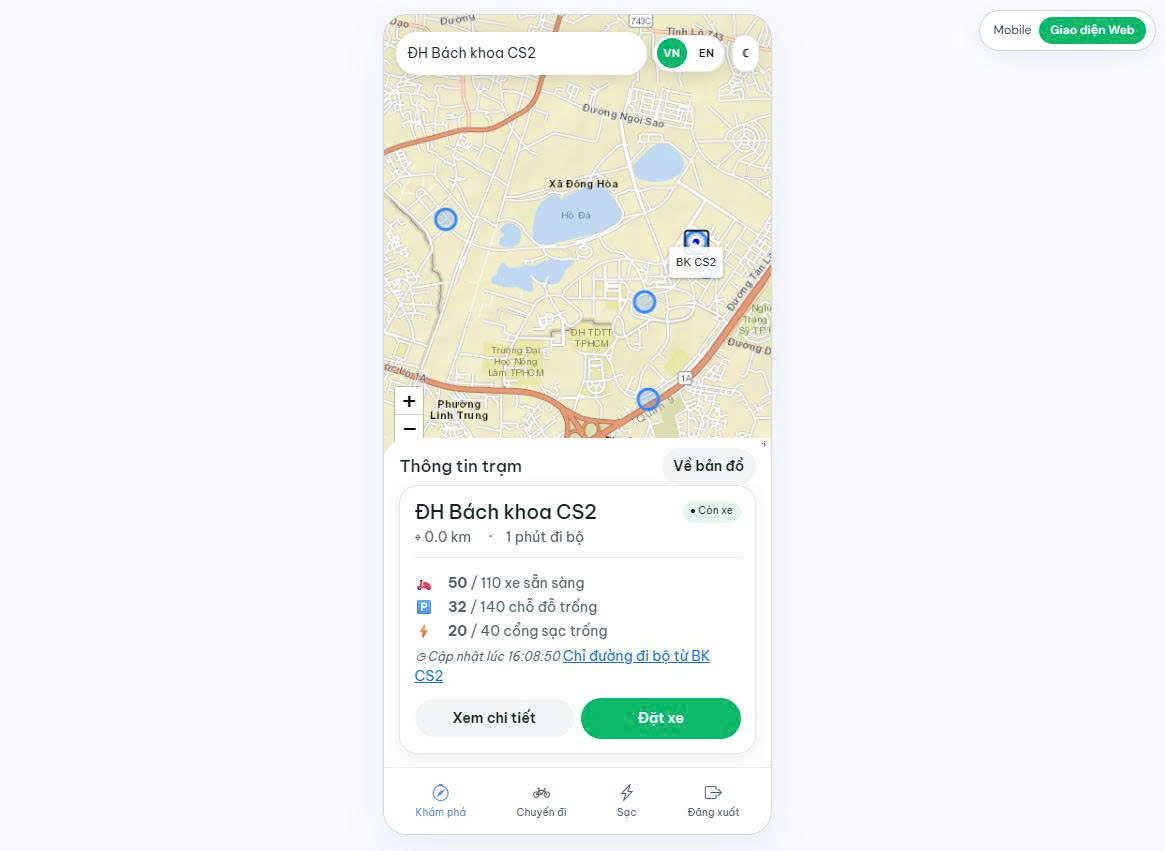
\includegraphics[width=0.88\textwidth]{demo_UC1-17/UC01_tim_phuong_tien_va_hub.jpg}
    \caption{UC1 --- Giao diện tìm kiếm phương tiện và bản đồ điều hướng tại Hub (\texttt{/student/search})}
    \label{fig:demo_uc01}
\end{figure}

\paragraph{UC2 --- Xem trạng thái phương tiện và Hub:}
Xem chi tiết số xe sẵn sàng, chỗ đỗ trống, cổng sạc và danh sách từng xe tại Hub kèm mức pin (\texttt{/student/resource}).
\begin{figure}[H]
    \centering
    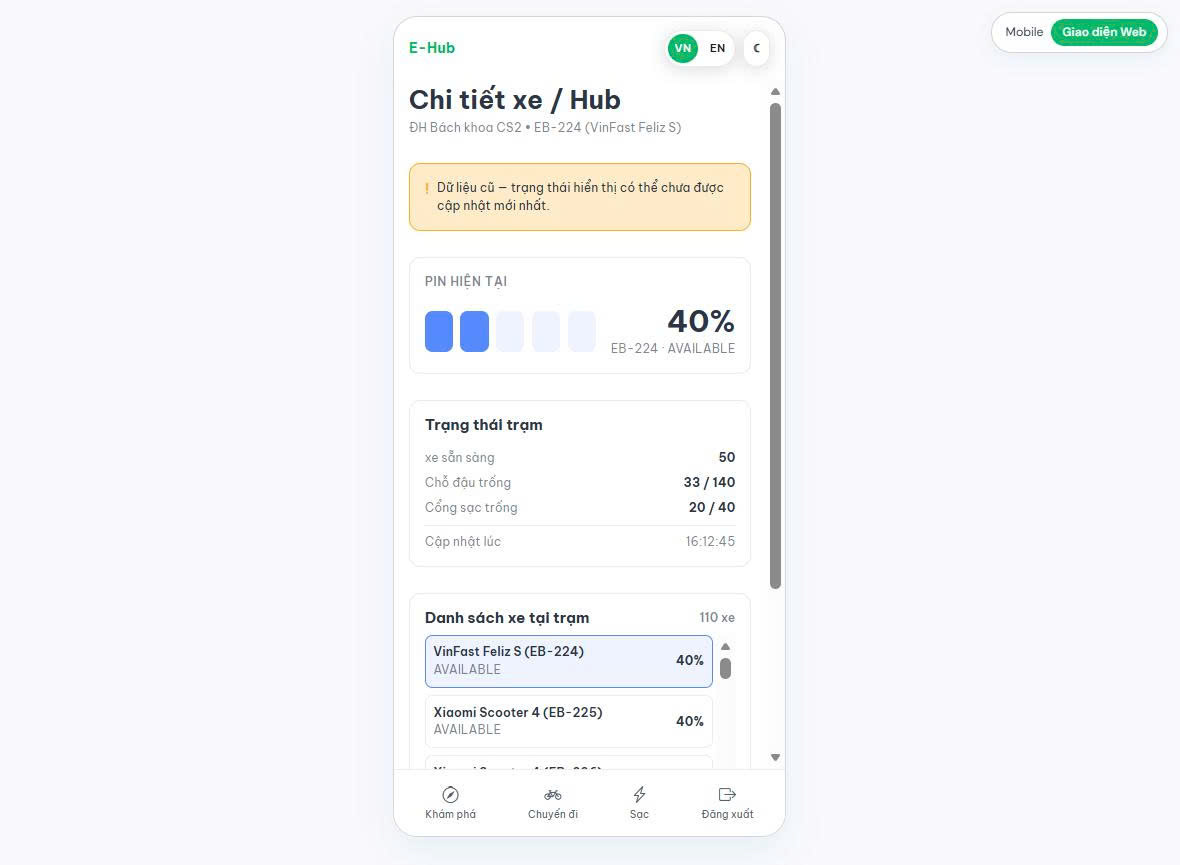
\includegraphics[width=0.88\textwidth]{demo_UC1-17/UC02_xem_trang_thai_phuong_tien_va_hub.jpg}
    \caption{UC2 --- Màn hình chi tiết trạng thái phương tiện và Hub (\texttt{/student/resource})}
    \label{fig:demo_uc02}
\end{figure}

\paragraph{UC3 --- Đặt xe:}
Sinh viên chọn phương tiện cụ thể trên modal đặt xe và nhận thông báo giữ xe thành công kèm mã đặt chỗ.
\begin{figure}[H]
    \centering
    \begin{subfigure}[b]{0.48\textwidth}
        \centering
        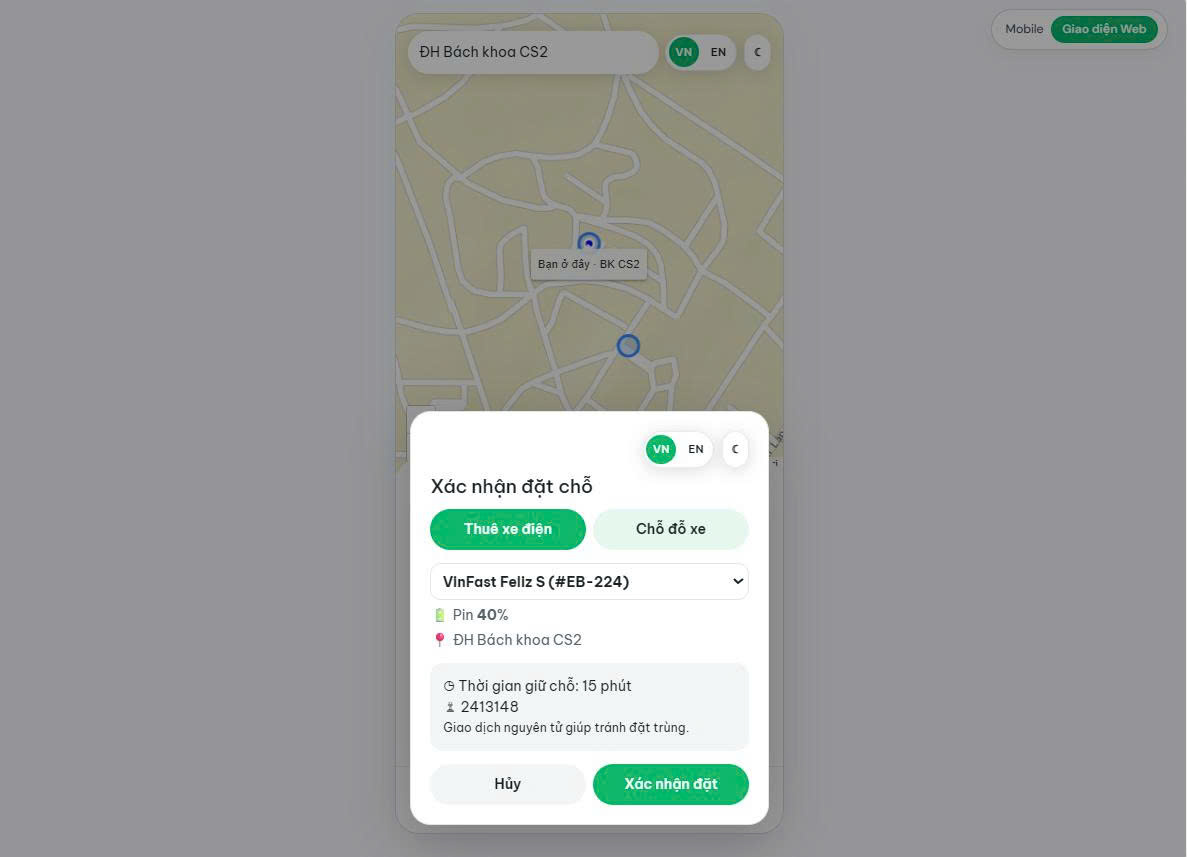
\includegraphics[width=\textwidth]{demo_UC1-17/UC03_dat_xe_1_form.jpg}
        \caption{Chọn xe và xác nhận thông tin đặt xe}
    \end{subfigure}
    \hfill
    \begin{subfigure}[b]{0.48\textwidth}
        \centering
        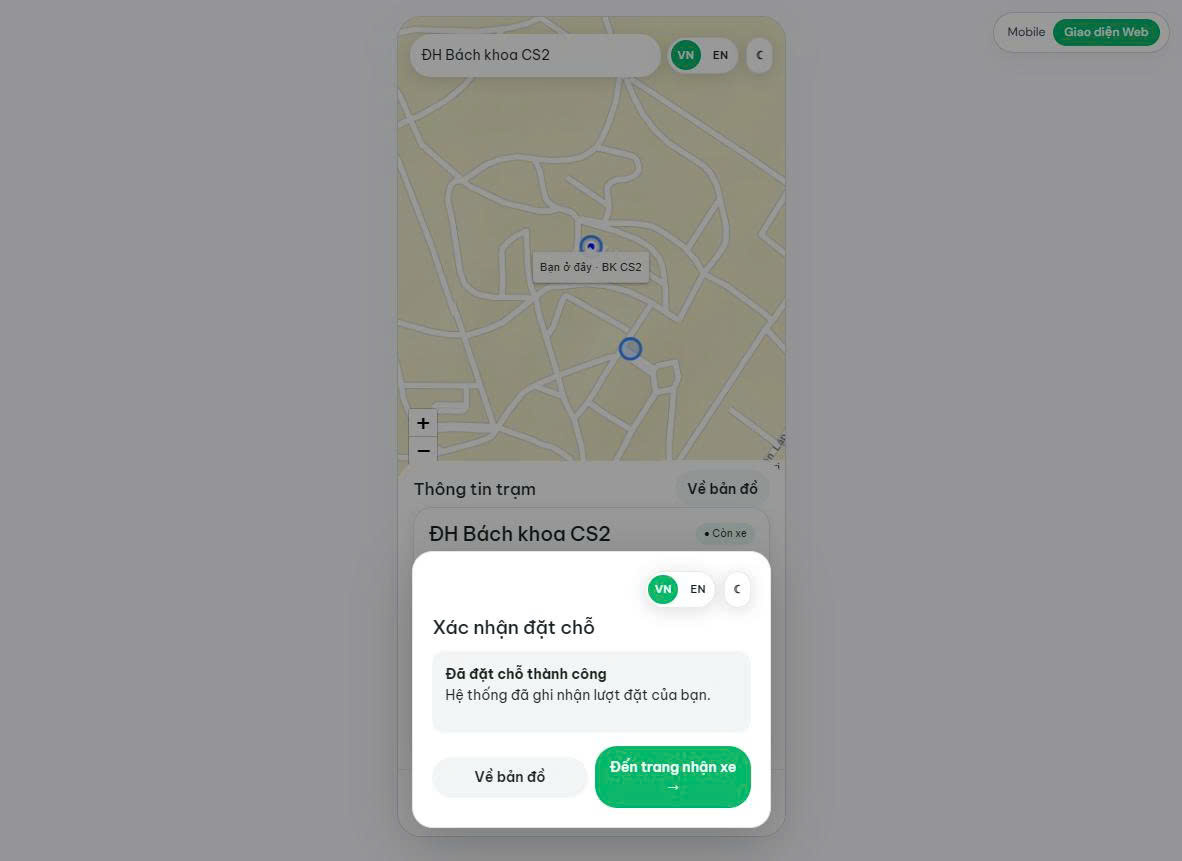
\includegraphics[width=\textwidth]{demo_UC1-17/UC03_dat_xe_2_thanh_cong.jpg}
        \caption{Đặt xe thành công và điều hướng nhận xe}
    \end{subfigure}
    \caption{UC3 --- Luồng đặt phương tiện trên cổng Sinh viên}
    \label{fig:demo_uc03}
\end{figure}

\paragraph{UC4 --- Đặt chỗ đỗ xe:}
Chức năng đặt trước chỗ đỗ theo khung giờ, kiểm tra chặn thời gian quá khứ và xác nhận đặt chỗ thành công.
\begin{figure}[H]
    \centering
    \begin{subfigure}[b]{0.48\textwidth}
        \centering
        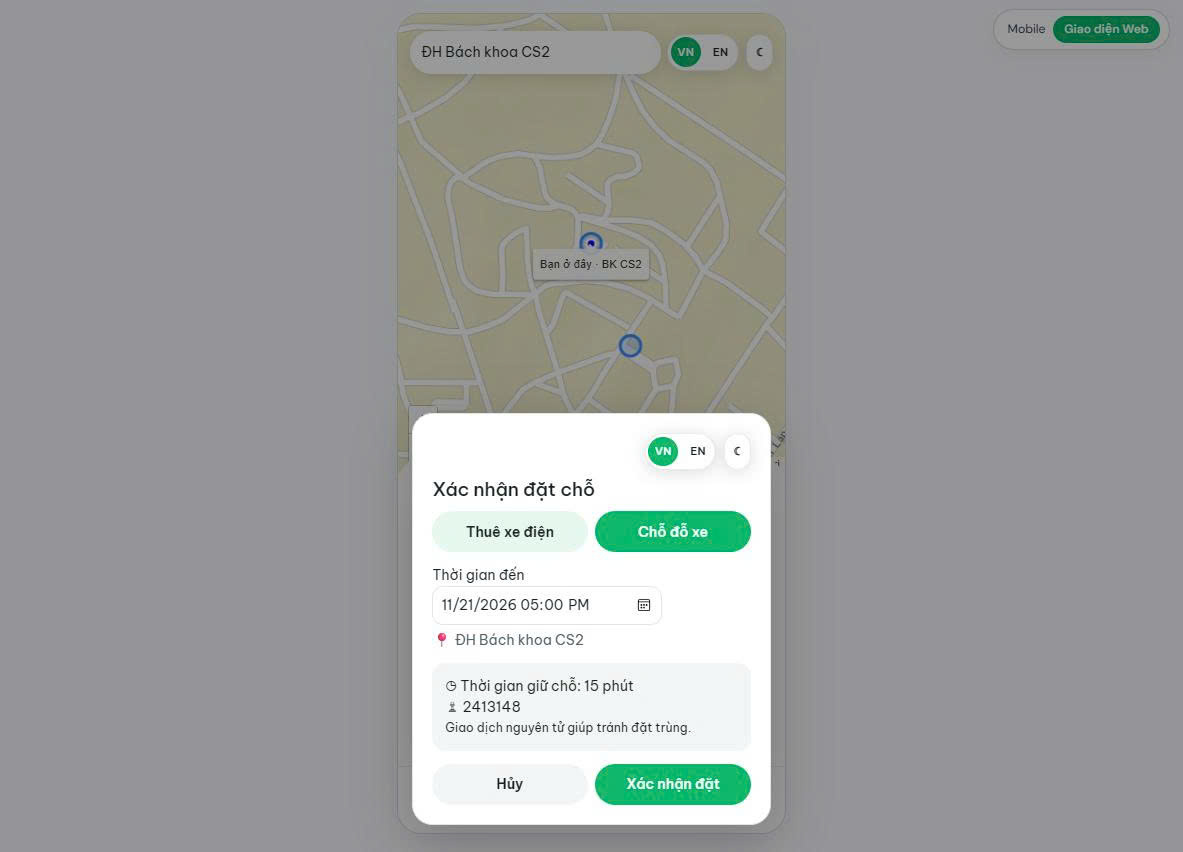
\includegraphics[width=\textwidth]{demo_UC1-17/UC04_dat_cho_do_xe_1_form.jpg}
        \caption{Chọn khung giờ đặt chỗ đỗ xe}
    \end{subfigure}
    \hfill
    \begin{subfigure}[b]{0.48\textwidth}
        \centering
        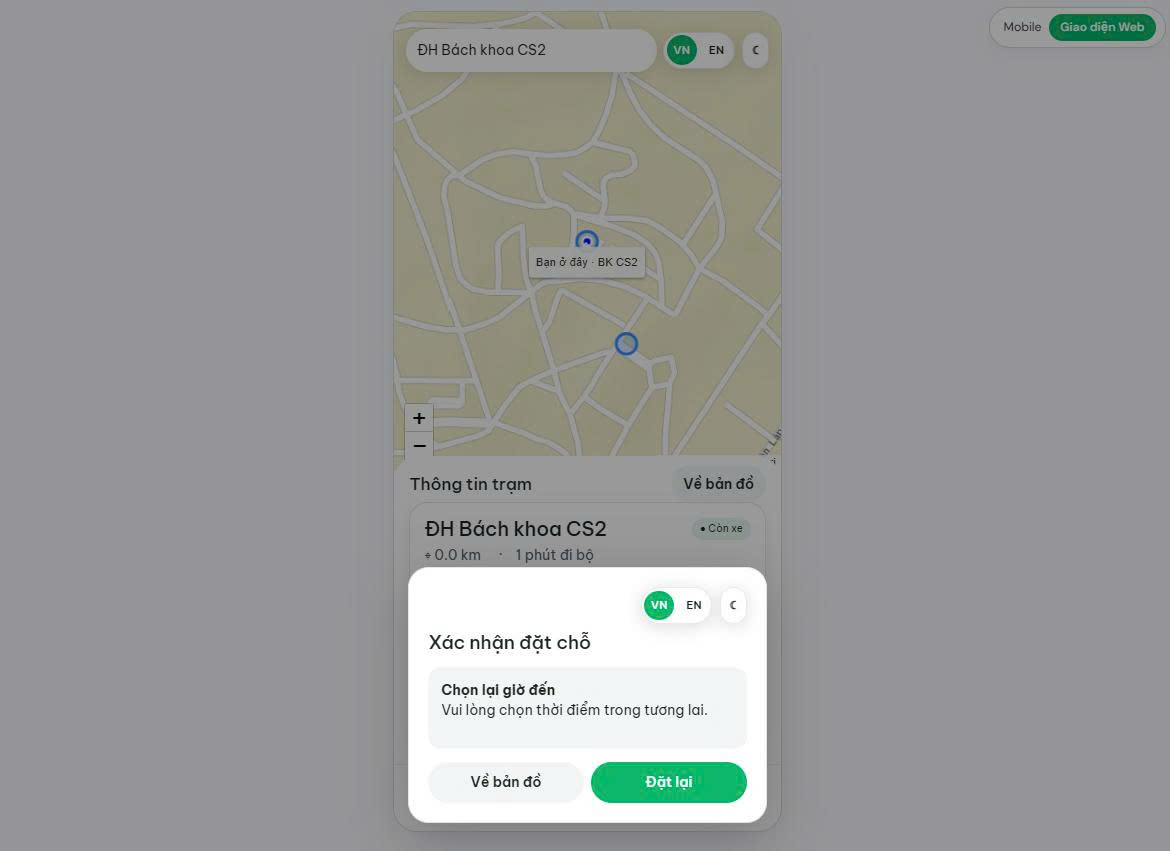
\includegraphics[width=\textwidth]{demo_UC1-17/UC04_dat_cho_do_xe_2_chan_gio_qua_khu.jpg}
        \caption{Ràng buộc chặn chọn giờ trong quá khứ}
    \end{subfigure}

    \vspace{0.3cm}
    \begin{subfigure}[b]{0.58\textwidth}
        \centering
        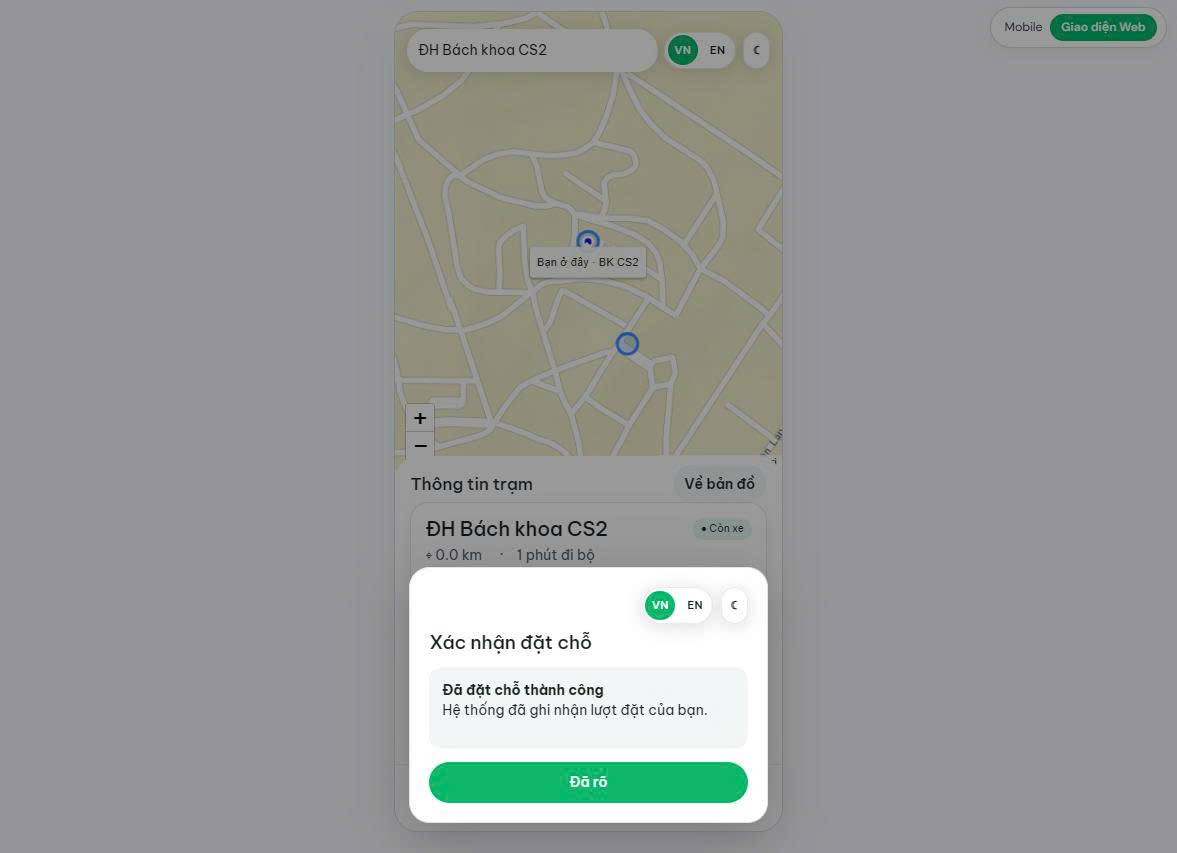
\includegraphics[width=\textwidth]{demo_UC1-17/UC04_dat_cho_do_xe_3_thanh_cong.jpg}
        \caption{Xác nhận đặt chỗ đỗ xe thành công}
    \end{subfigure}
    \caption{UC4 --- Luồng đặt chỗ đỗ xe và kiểm tra ràng buộc thời gian}
    \label{fig:demo_uc04}
\end{figure}

\paragraph{UC5 --- Nhận phương tiện:}
Sinh viên xác nhận nhận xe đã đặt tại trạm (\texttt{/student/pickup}) để chuyển trạng thái sang chuyến đi đang hoạt động (\texttt{/student/ride}).
\begin{figure}[H]
    \centering
    \begin{subfigure}[b]{0.48\textwidth}
        \centering
        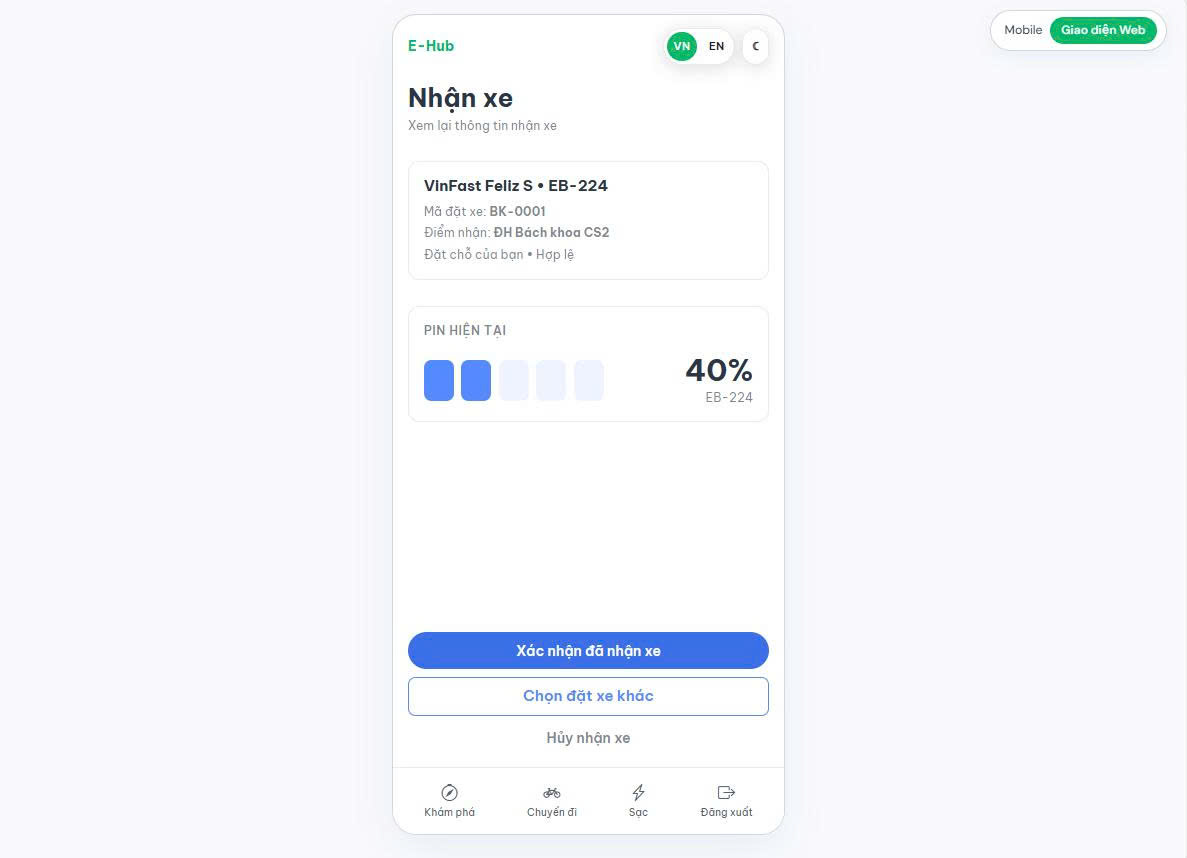
\includegraphics[width=\textwidth]{demo_UC1-17/UC05_nhan_phuong_tien_1_xac_nhan.jpg}
        \caption{Xác nhận thông tin trước khi nhận xe}
    \end{subfigure}
    \hfill
    \begin{subfigure}[b]{0.48\textwidth}
        \centering
        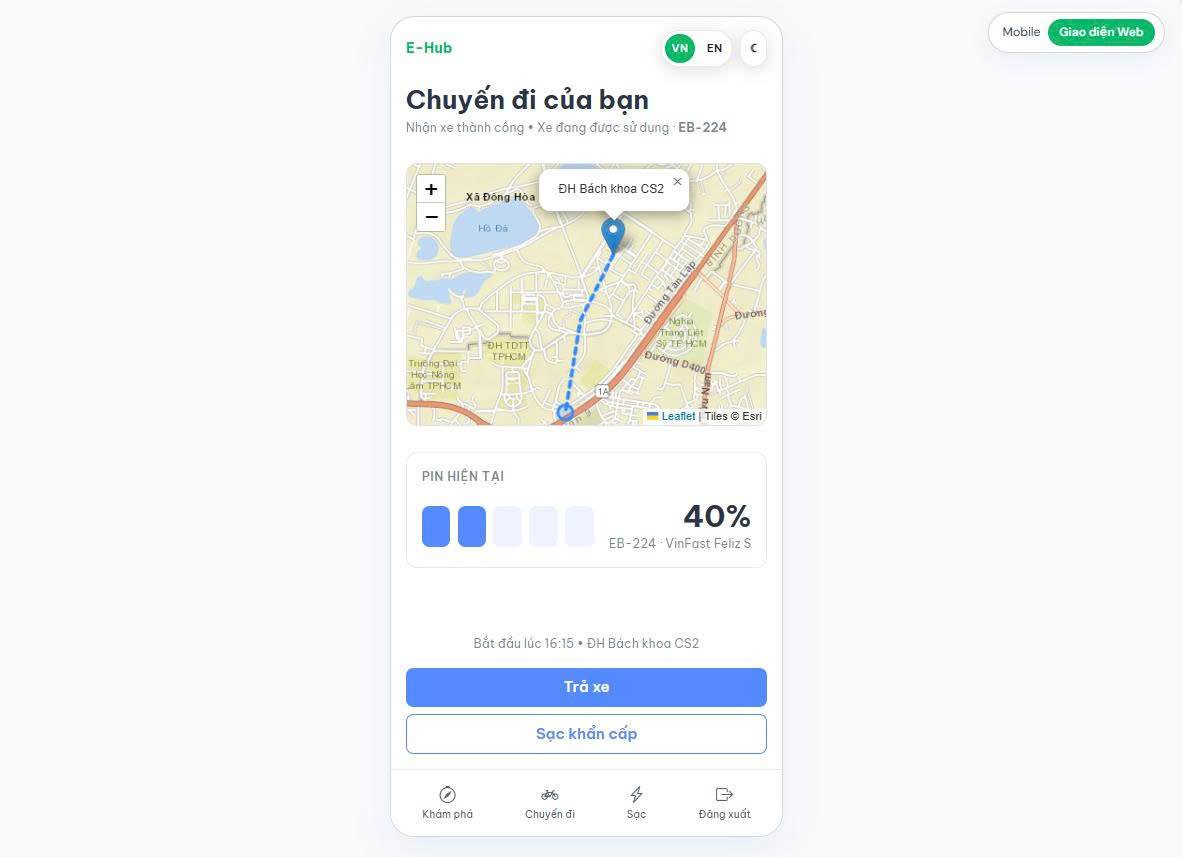
\includegraphics[width=\textwidth]{demo_UC1-17/UC05_nhan_phuong_tien_2_chuyen_di.jpg}
        \caption{Chuyến đi bắt đầu kèm bản đồ và mức pin}
    \end{subfigure}
    \caption{UC5 --- Xác nhận nhận phương tiện và theo dõi chuyến đi}
    \label{fig:demo_uc05}
\end{figure}

\paragraph{UC6 --- Trả phương tiện:}
Chọn trạm trả xe còn chỗ trống (\texttt{/student/return}) và hoàn tất giao dịch trả xe (\texttt{/student/returned}).
\begin{figure}[H]
    \centering
    \begin{subfigure}[b]{0.48\textwidth}
        \centering
        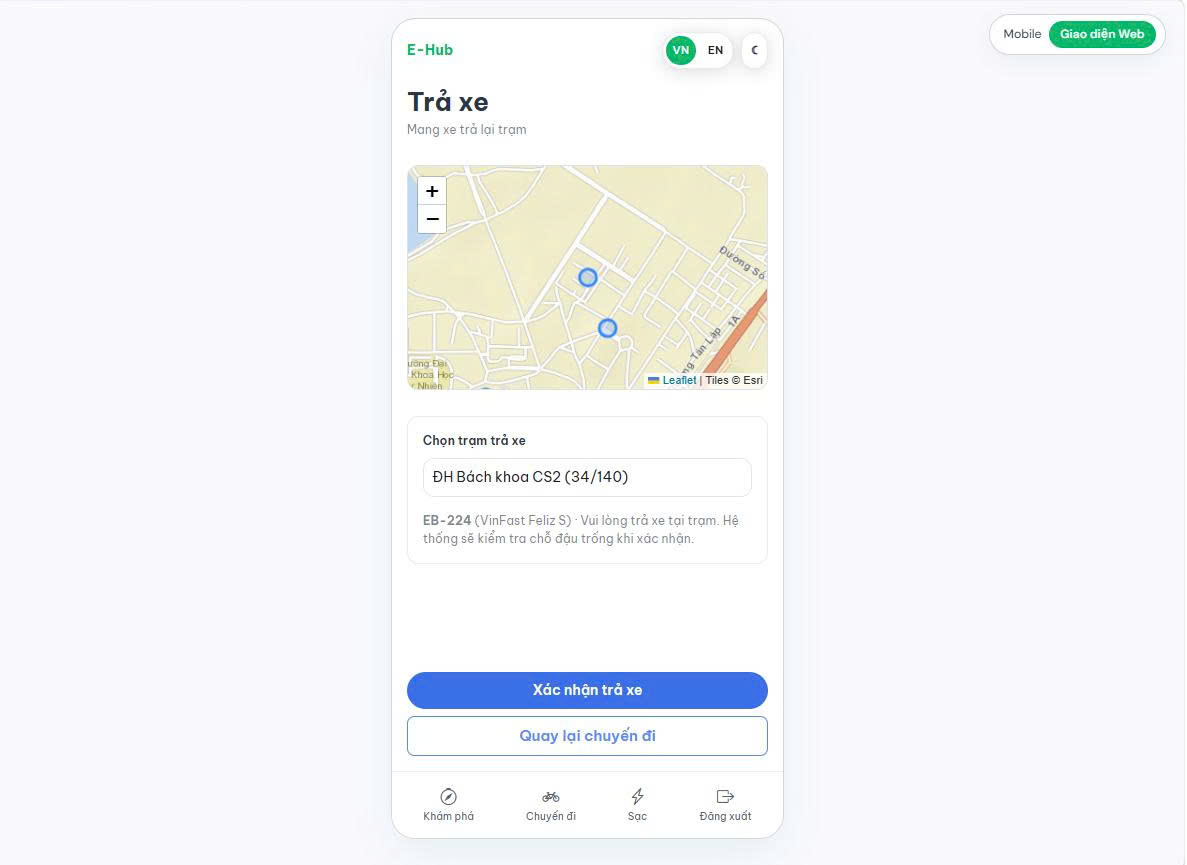
\includegraphics[width=\textwidth]{demo_UC1-17/UC06_tra_phuong_tien_1_form.jpg}
        \caption{Chọn trạm trả xe trên giao diện trả xe}
    \end{subfigure}
    \hfill
    \begin{subfigure}[b]{0.48\textwidth}
        \centering
        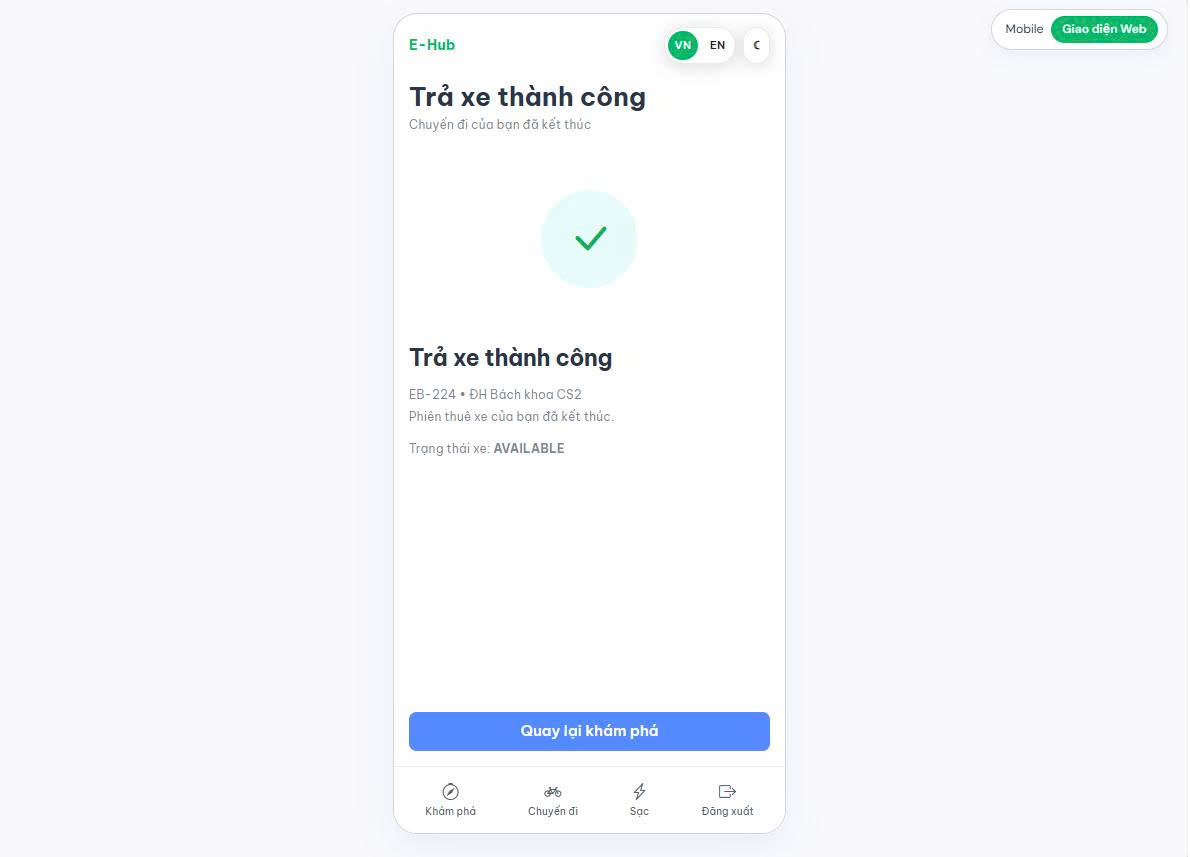
\includegraphics[width=\textwidth]{demo_UC1-17/UC06_tra_phuong_tien_2_thanh_cong.jpg}
        \caption{Thông báo trả phương tiện thành công}
    \end{subfigure}
    \caption{UC6 --- Luồng trả phương tiện tại Hub}
    \label{fig:demo_uc06}
\end{figure}

\paragraph{UC7 --- Đăng ký sạc:}
Hỗ trợ gợi ý trạm sạc khẩn cấp gần nhất, chọn khung giờ sạc khả dụng, xem lại thông tin và hoàn tất đăng ký cổng sạc.
\begin{figure}[H]
    \centering
    \begin{subfigure}[b]{0.46\textwidth}
        \centering
        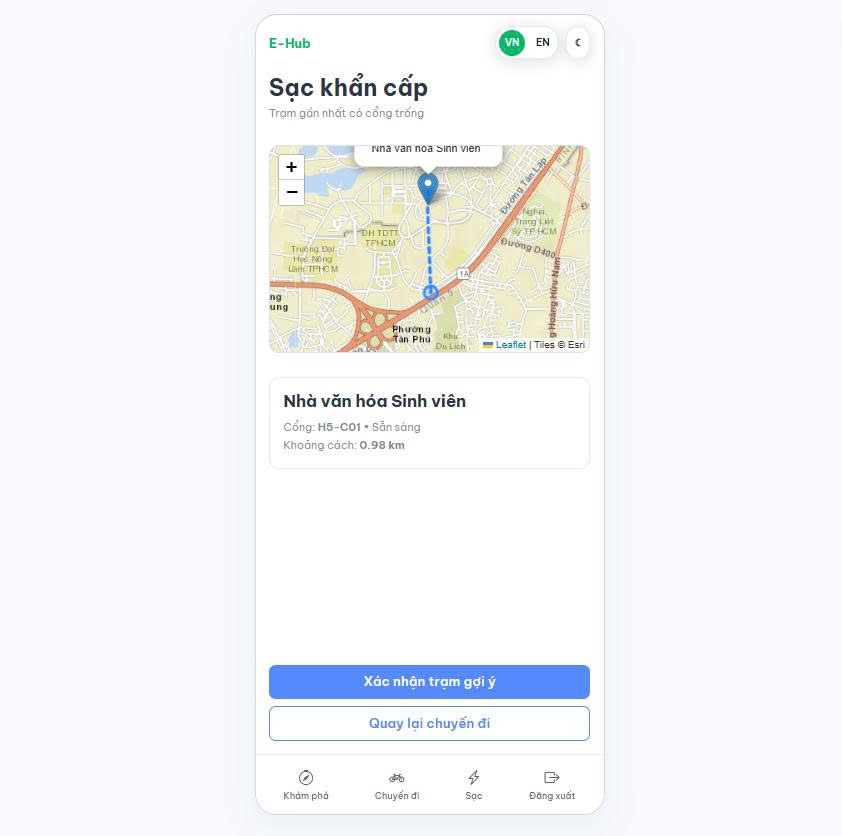
\includegraphics[width=\textwidth]{demo_UC1-17/UC07_dang_ky_sac_1_sac_khan_cap.jpg}
        \caption{Gợi ý trạm sạc khẩn cấp gần nhất}
    \end{subfigure}
    \hfill
    \begin{subfigure}[b]{0.46\textwidth}
        \centering
        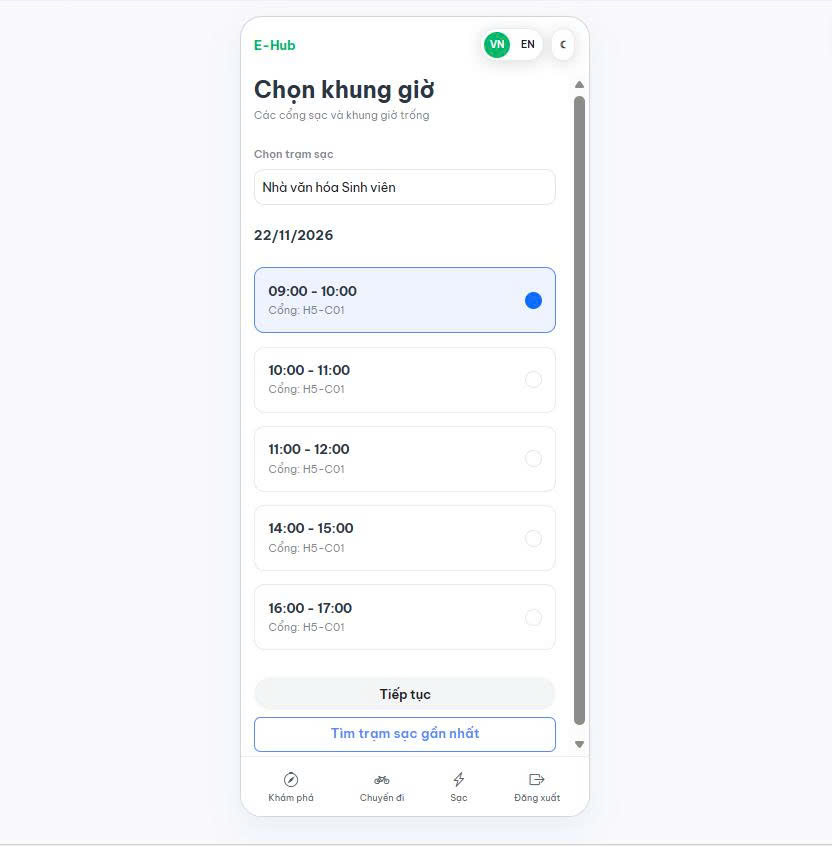
\includegraphics[width=\textwidth]{demo_UC1-17/UC07_dang_ky_sac_2_chon_gio.jpg}
        \caption{Chọn Hub và khung giờ sạc}
    \end{subfigure}

    \vspace{0.3cm}
    \begin{subfigure}[b]{0.46\textwidth}
        \centering
        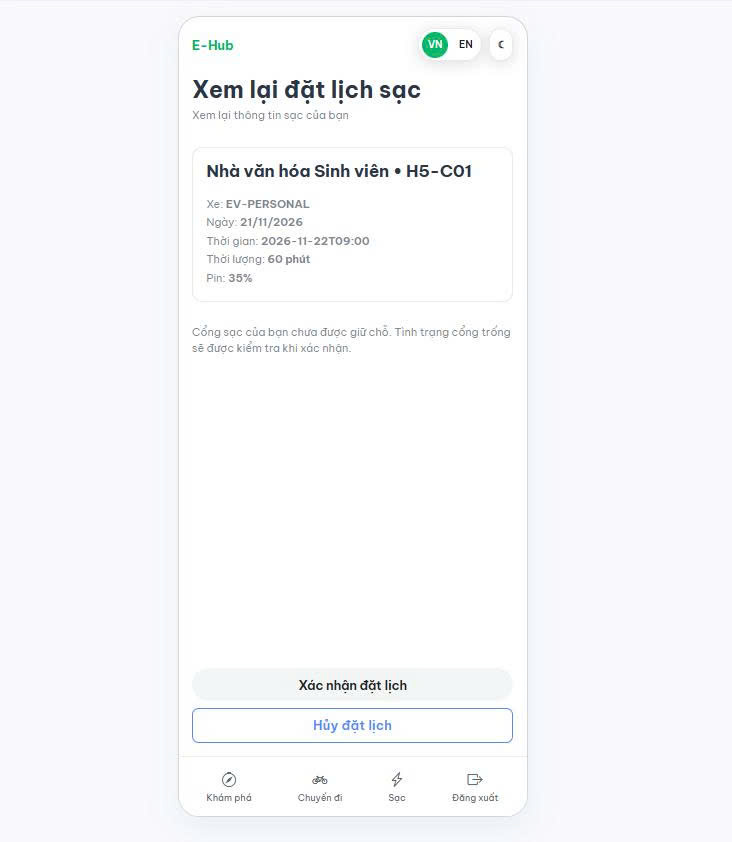
\includegraphics[width=\textwidth]{demo_UC1-17/UC07_dang_ky_sac_3_xem_lai.jpg}
        \caption{Xem lại thông tin trước khi xác nhận}
    \end{subfigure}
    \hfill
    \begin{subfigure}[b]{0.46\textwidth}
        \centering
        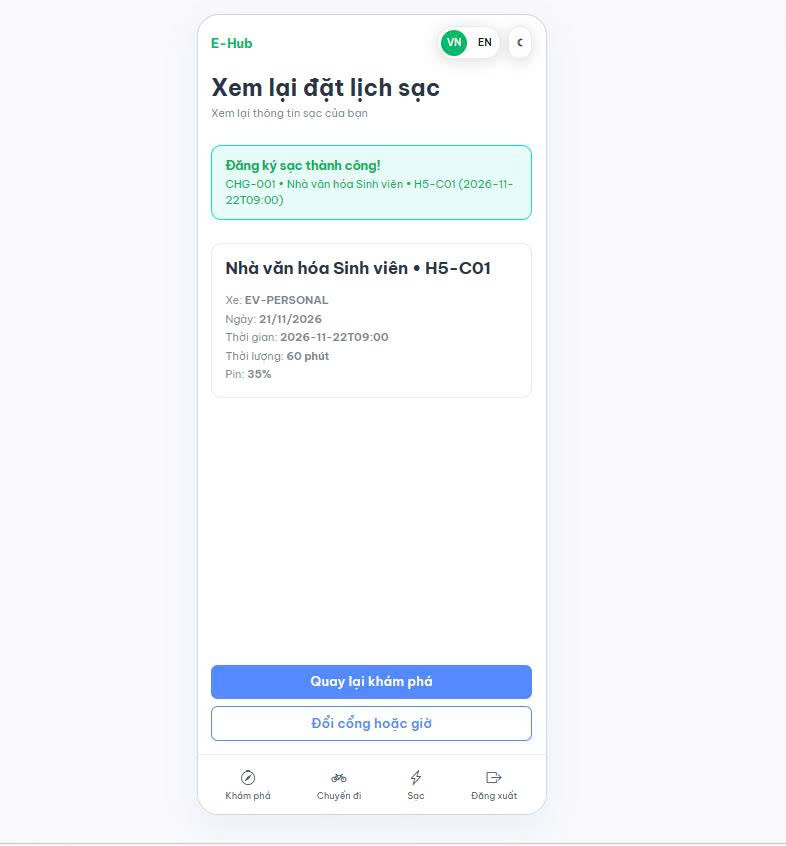
\includegraphics[width=\textwidth]{demo_UC1-17/UC07_dang_ky_sac_4_thanh_cong.jpg}
        \caption{Đăng ký khung giờ sạc thành công}
    \end{subfigure}
    \caption{UC7 --- Chuỗi màn hình gợi ý sạc khẩn cấp và đăng ký lịch sạc}
    \label{fig:demo_uc07}
\end{figure}

\paragraph{UC15 --- Tùy chỉnh giao diện:}
Chuyển đổi trực tiếp giữa chế độ Sáng/Tối (Light/Dark Mode) và song ngữ Việt/Anh (VN/EN) mà không tải lại trang.
\begin{figure}[H]
    \centering
    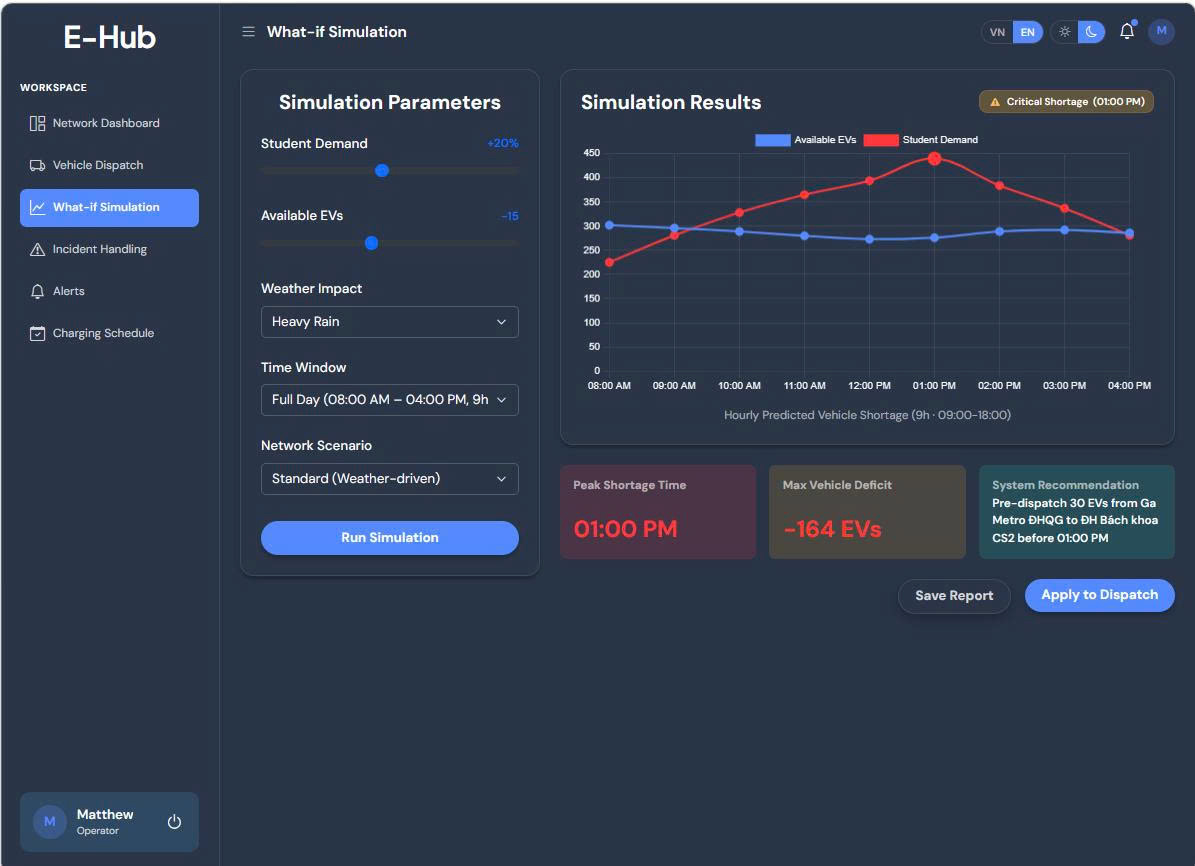
\includegraphics[width=0.88\textwidth]{demo_UC1-17/UC15_tuy_chinh_giao_dien_dark_en.jpg}
    \caption{UC15 --- Giao diện hệ thống ở chế độ Nền tối (Dark Mode) và Tiếng Anh (EN)}
    \label{fig:demo_uc15}
\end{figure}

\paragraph{UC17 --- Xác thực SSO Dual-Portal:}
Tách biệt hoàn toàn cổng đăng nhập cho Sinh viên (\texttt{/login}) và Đơn vị vận hành (\texttt{/operator/login}), kiểm tra phân quyền theo vai trò tài khoản.
\begin{figure}[H]
    \centering
    \begin{subfigure}[b]{0.48\textwidth}
        \centering
        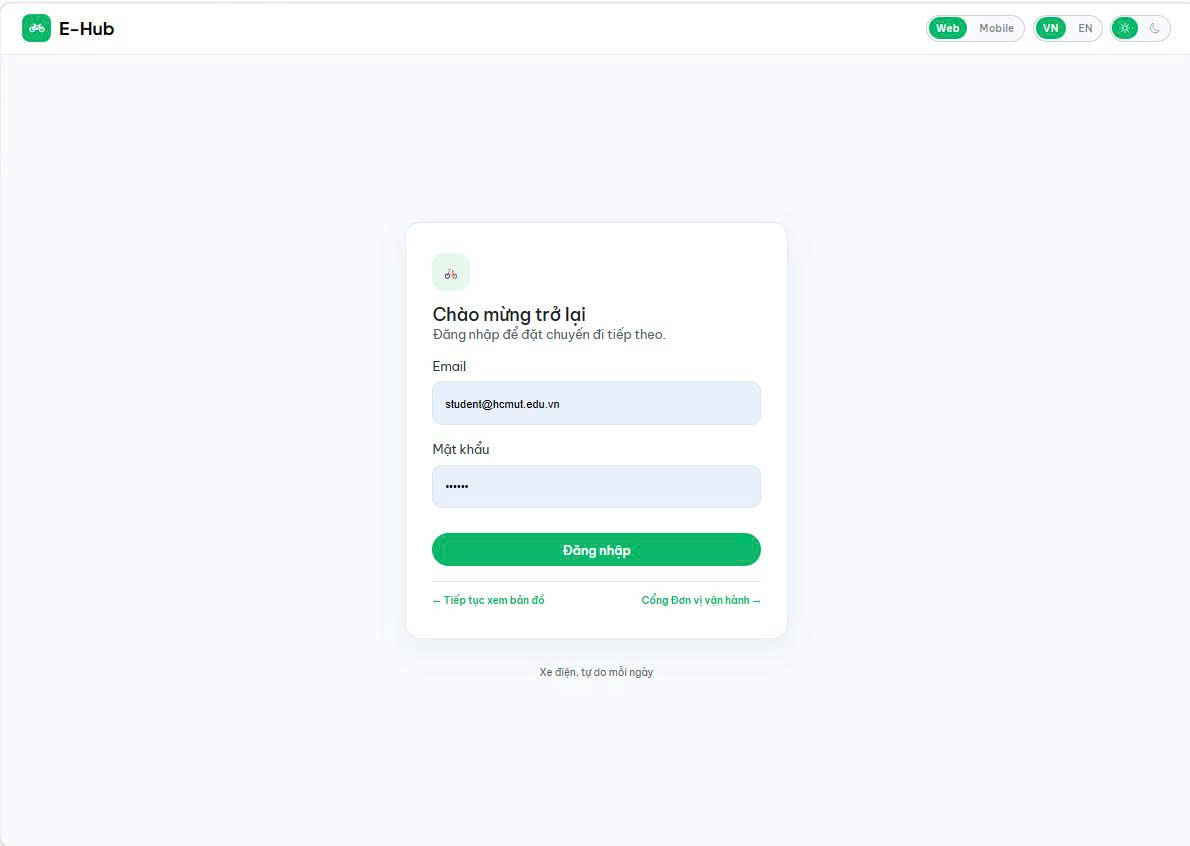
\includegraphics[width=\textwidth]{demo_UC1-17/UC17_xac_thuc_sso_1_student.jpg}
        \caption{Cổng đăng nhập SSO dành cho Sinh viên}
    \end{subfigure}
    \hfill
    \begin{subfigure}[b]{0.48\textwidth}
        \centering
        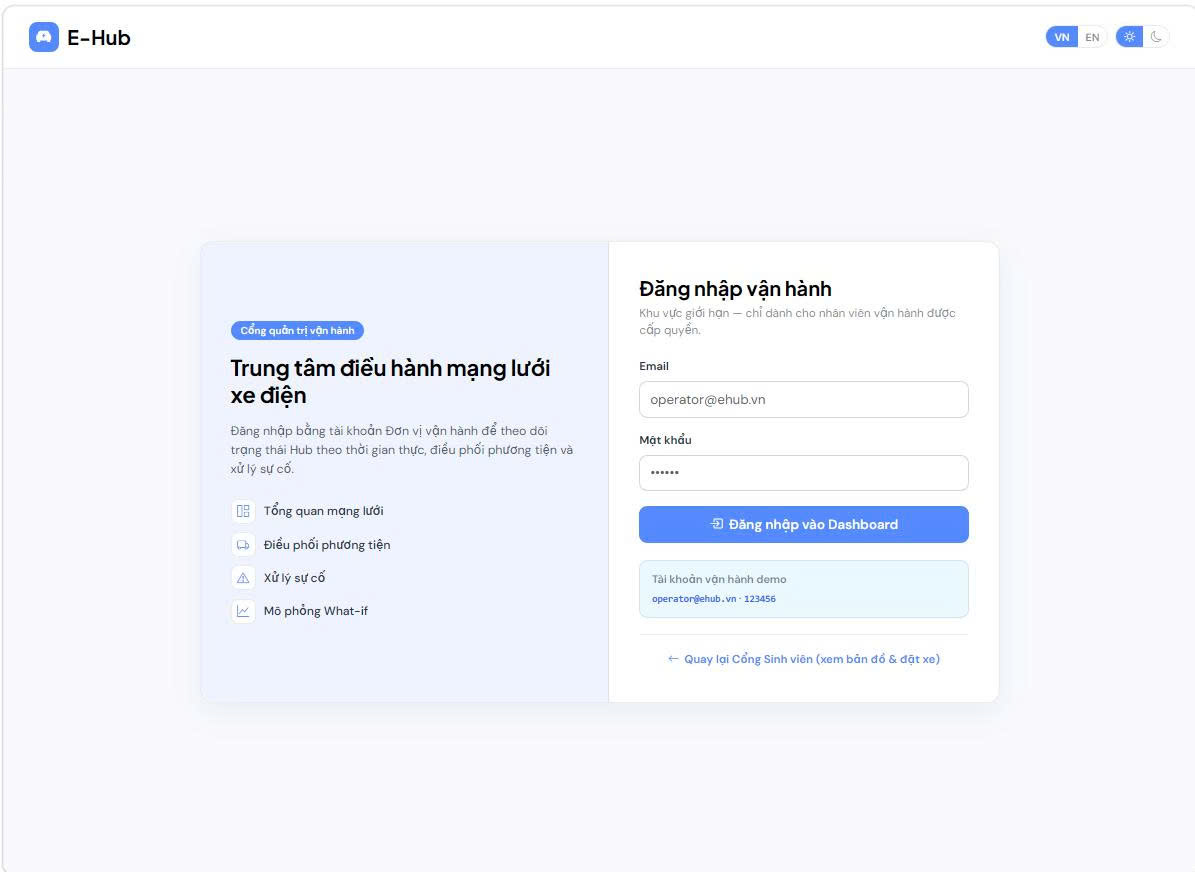
\includegraphics[width=\textwidth]{demo_UC1-17/UC17_xac_thuc_sso_2_operator.jpg}
        \caption{Cổng đăng nhập riêng cho Operator}
    \end{subfigure}
    \caption{UC17 --- Xác thực SSO tách biệt hai phân hệ (Dual-Portal Login)}
    \label{fig:demo_uc17}
\end{figure}

\subsubsection{Phân hệ Đơn vị vận hành (Operator)}

\paragraph{UC8 --- Giám sát mạng lưới Hub:}
Trang tổng quan Dashboard (\texttt{/operator/overview}) hiển thị các chỉ số KPI toàn mạng, bảng tải 5 Hub cập nhật thời gian thực và cảnh báo nổi bật.
\begin{figure}[H]
    \centering
    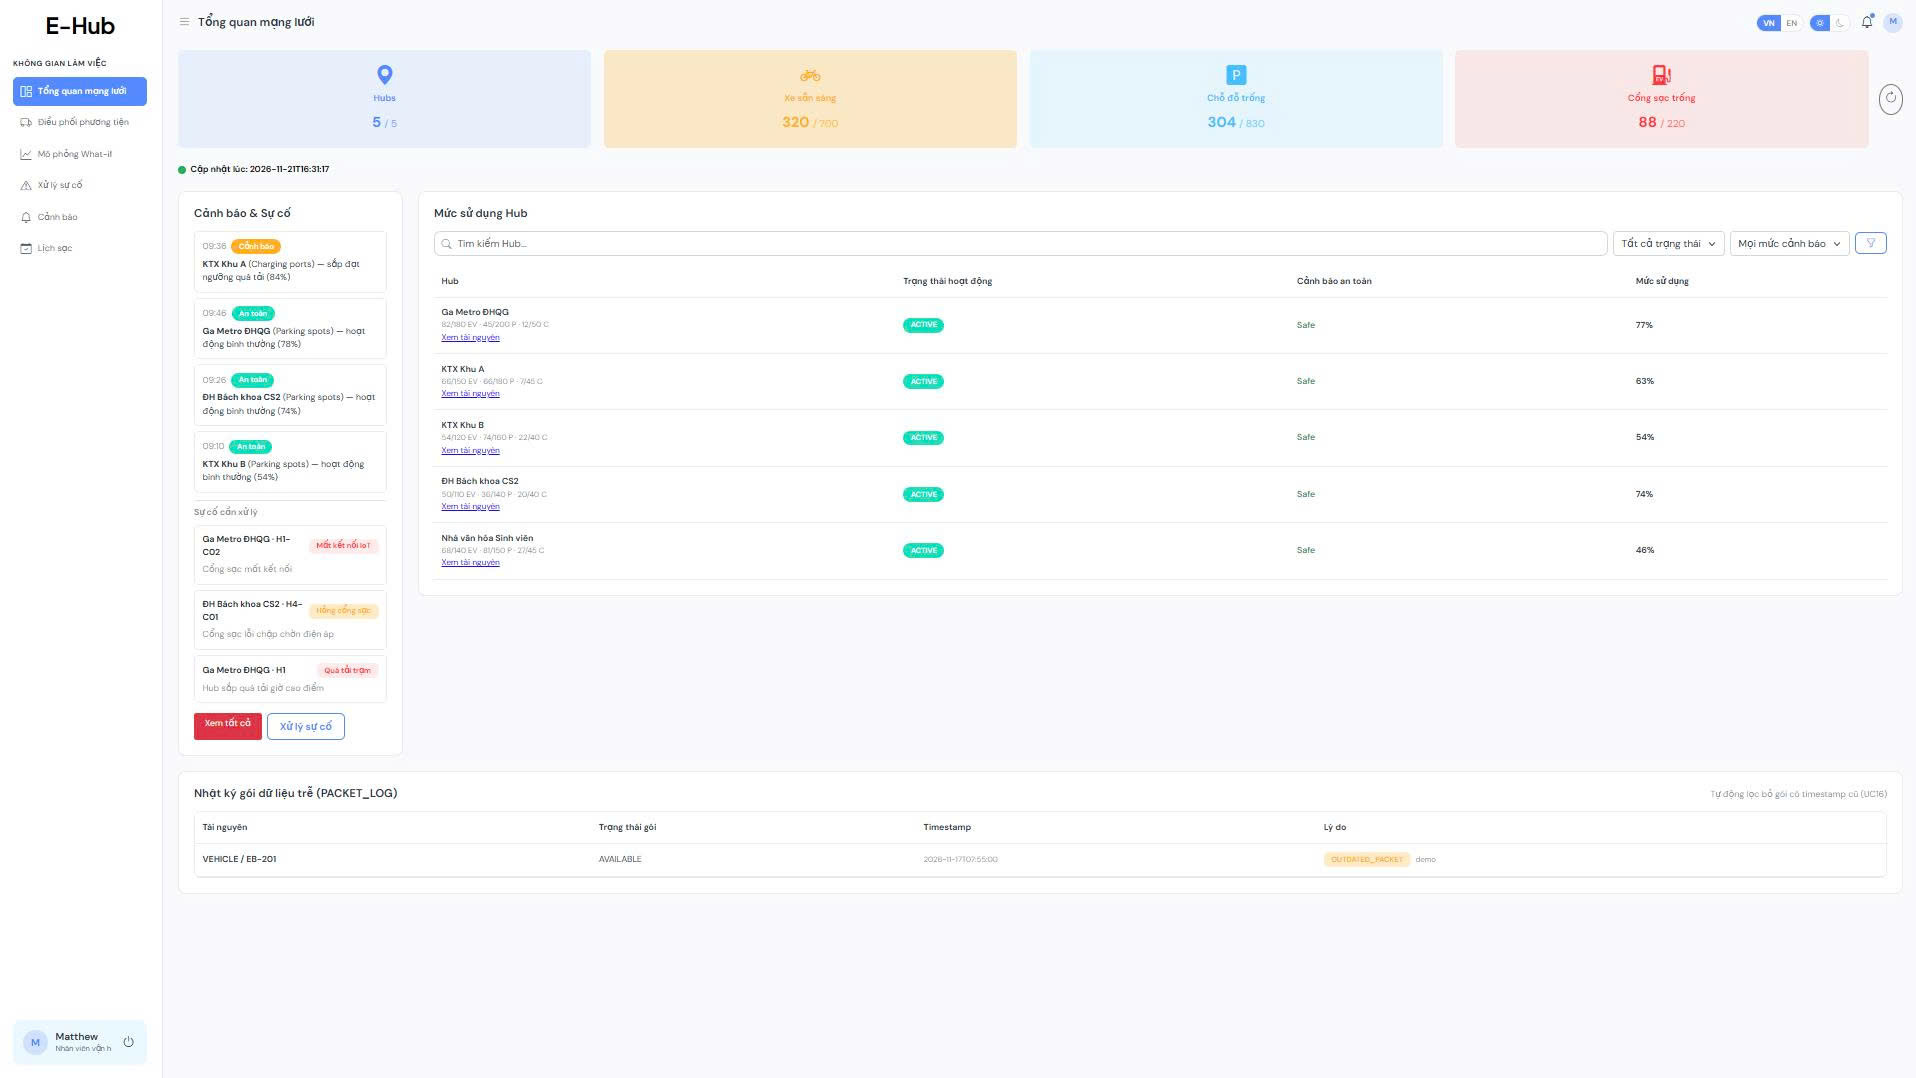
\includegraphics[width=0.92\textwidth]{demo_UC1-17/UC08_giam_sat_mang_luoi_hub.jpg}
    \caption{UC8 --- Bảng điều khiển tổng quan mạng lưới Hub (\texttt{/operator/overview})}
    \label{fig:demo_uc08}
\end{figure}

\paragraph{UC9 --- Theo dõi tài nguyên Hub:}
Quản lý tập trung trạng thái của 700 phương tiện, 830 chỗ đỗ và 220 cổng sạc kèm thanh tìm kiếm và bộ lọc theo Hub (\texttt{/operator/resources}).
\begin{figure}[H]
    \centering
    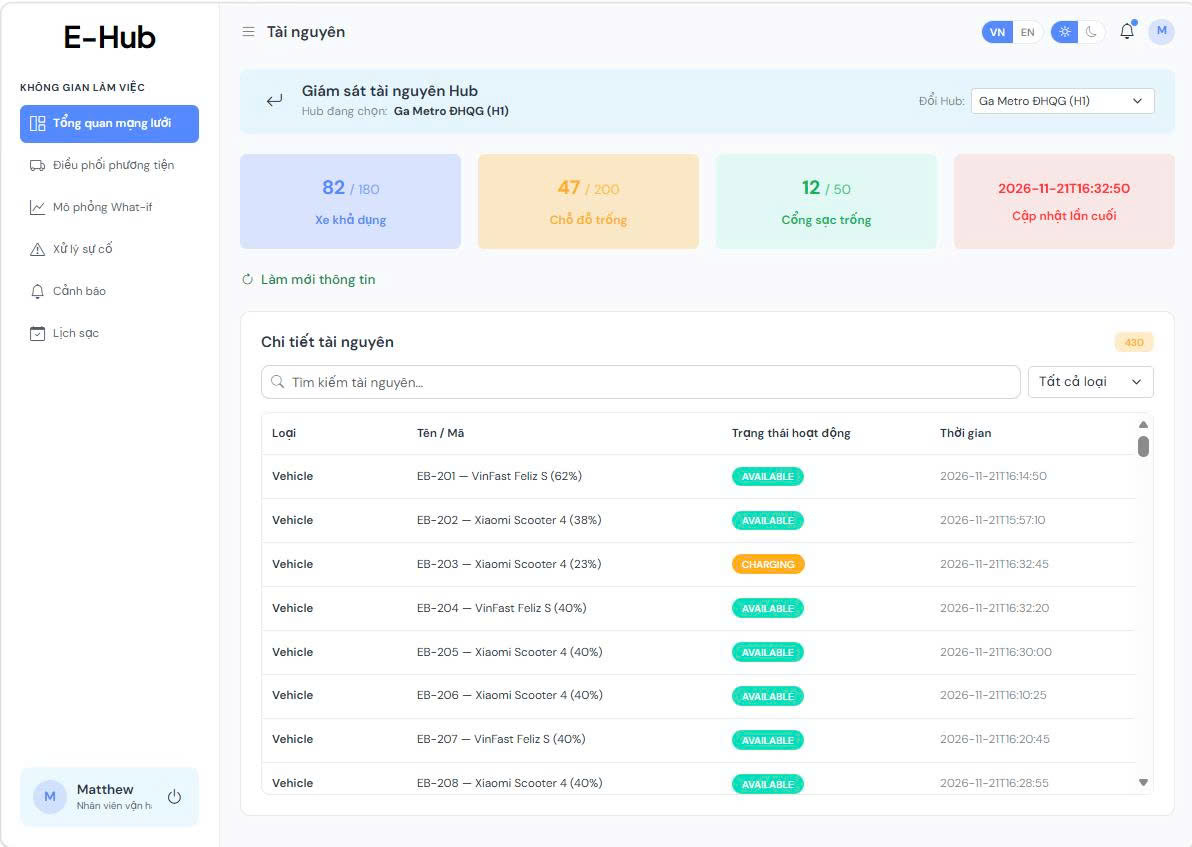
\includegraphics[width=0.88\textwidth]{demo_UC1-17/UC09_theo_doi_tai_nguyen.jpg}
    \caption{UC9 --- Màn hình theo dõi tài nguyên từng Hub (\texttt{/operator/resources})}
    \label{fig:demo_uc09}
\end{figure}

\paragraph{UC10 --- Cảnh báo quá tải:}
Hiển thị danh sách cảnh báo quá tải phân loại theo 3 mức độ nghiêm trọng (\texttt{HIGH}, \texttt{MEDIUM}, \texttt{LOW}) để vận hành ưu tiên xử lý (\texttt{/operator/alerts}).
\begin{figure}[H]
    \centering
    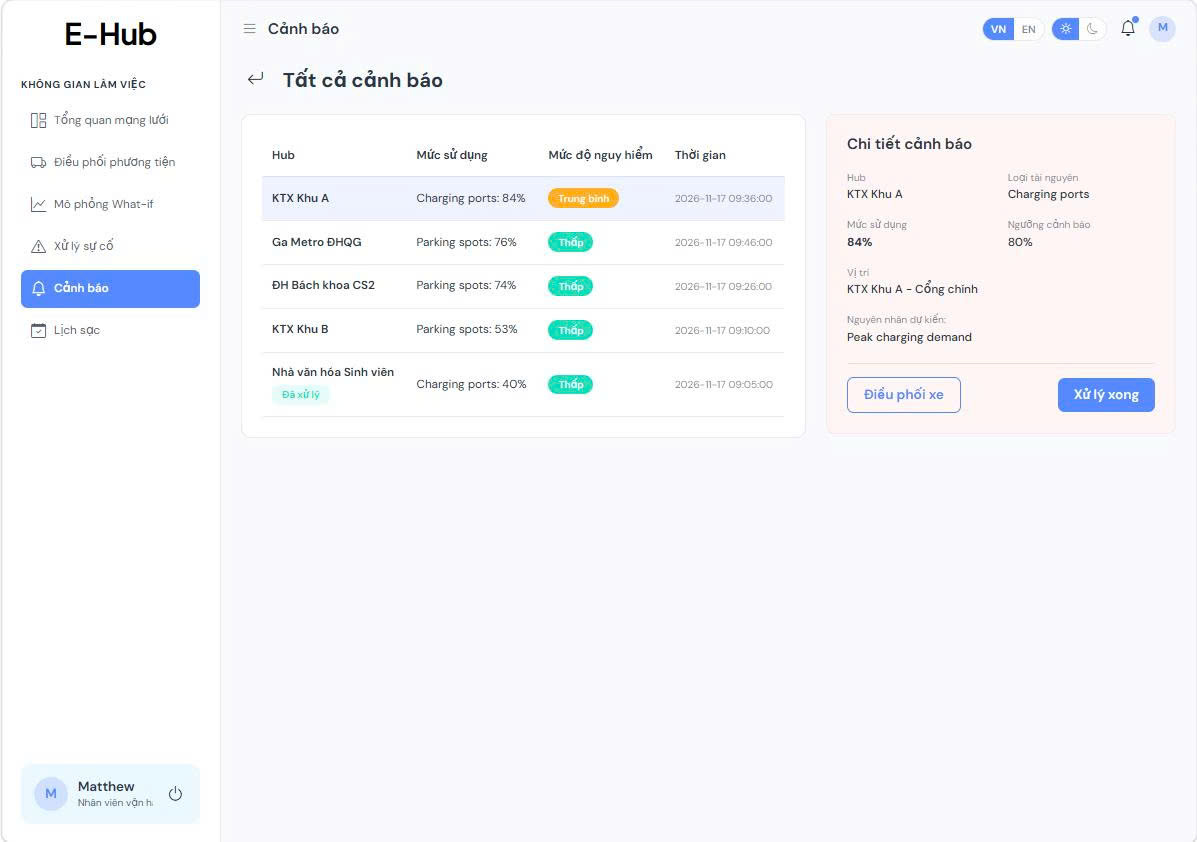
\includegraphics[width=0.88\textwidth]{demo_UC1-17/UC10_xem_canh_bao_qua_tai.jpg}
    \caption{UC10 --- Màn hình cảnh báo quá tải tại các Hub (\texttt{/operator/alerts})}
    \label{fig:demo_uc10}
\end{figure}

\paragraph{UC11 --- Điều phối phương tiện:}
Operator chọn Hub nguồn/đích trực tiếp trên bản đồ Leaflet (\texttt{/operator/dispatch}), chọn các xe cần chuyển và tạo lệnh điều phối.
\begin{figure}[H]
    \centering
    \begin{subfigure}[b]{0.48\textwidth}
        \centering
        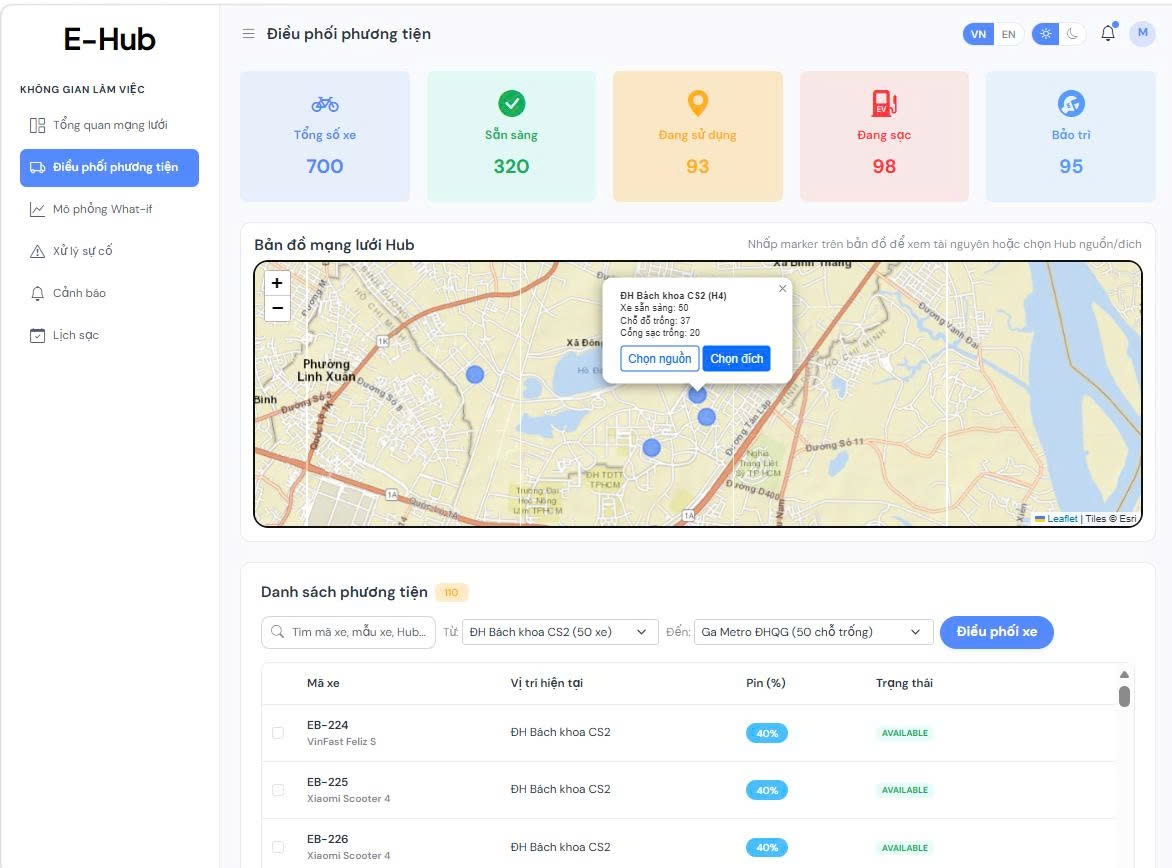
\includegraphics[width=\textwidth]{demo_UC1-17/UC11_dieu_phoi_phuong_tien_1_chon_hub.jpg}
        \caption{Chọn Hub nguồn và đích trên bản đồ}
    \end{subfigure}
    \hfill
    \begin{subfigure}[b]{0.48\textwidth}
        \centering
        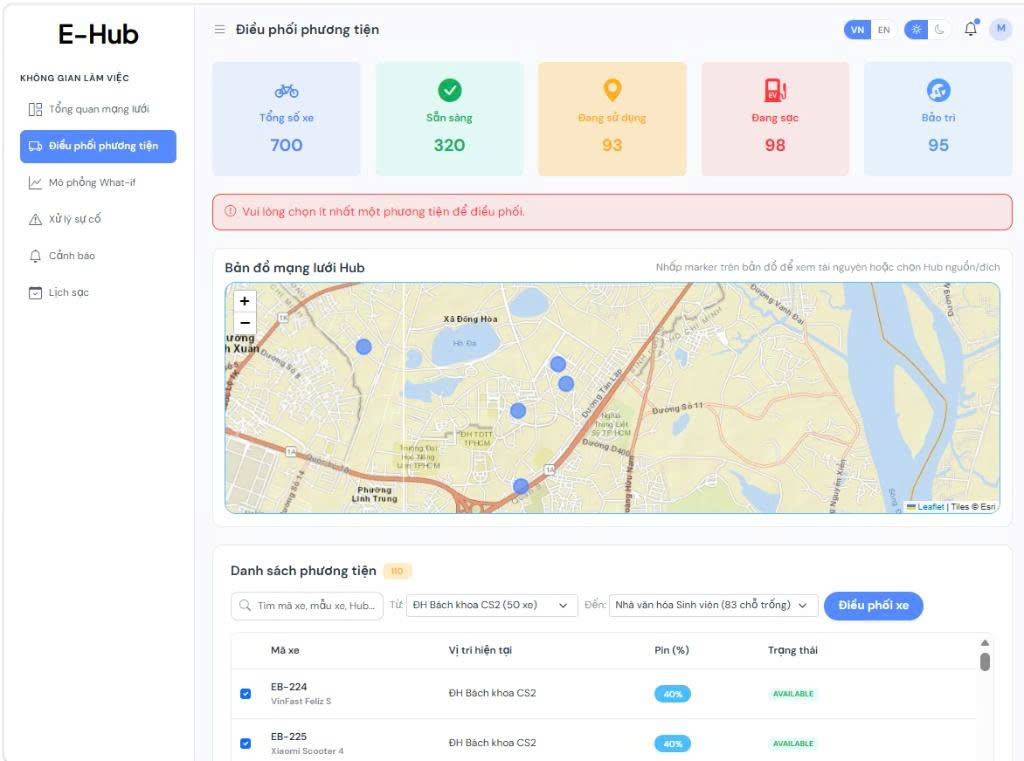
\includegraphics[width=\textwidth]{demo_UC1-17/UC11_dieu_phoi_phuong_tien_2_chon_xe.jpg}
        \caption{Chọn danh sách phương tiện cần điều phối}
    \end{subfigure}

    \vspace{0.3cm}
    \begin{subfigure}[b]{0.68\textwidth}
        \centering
        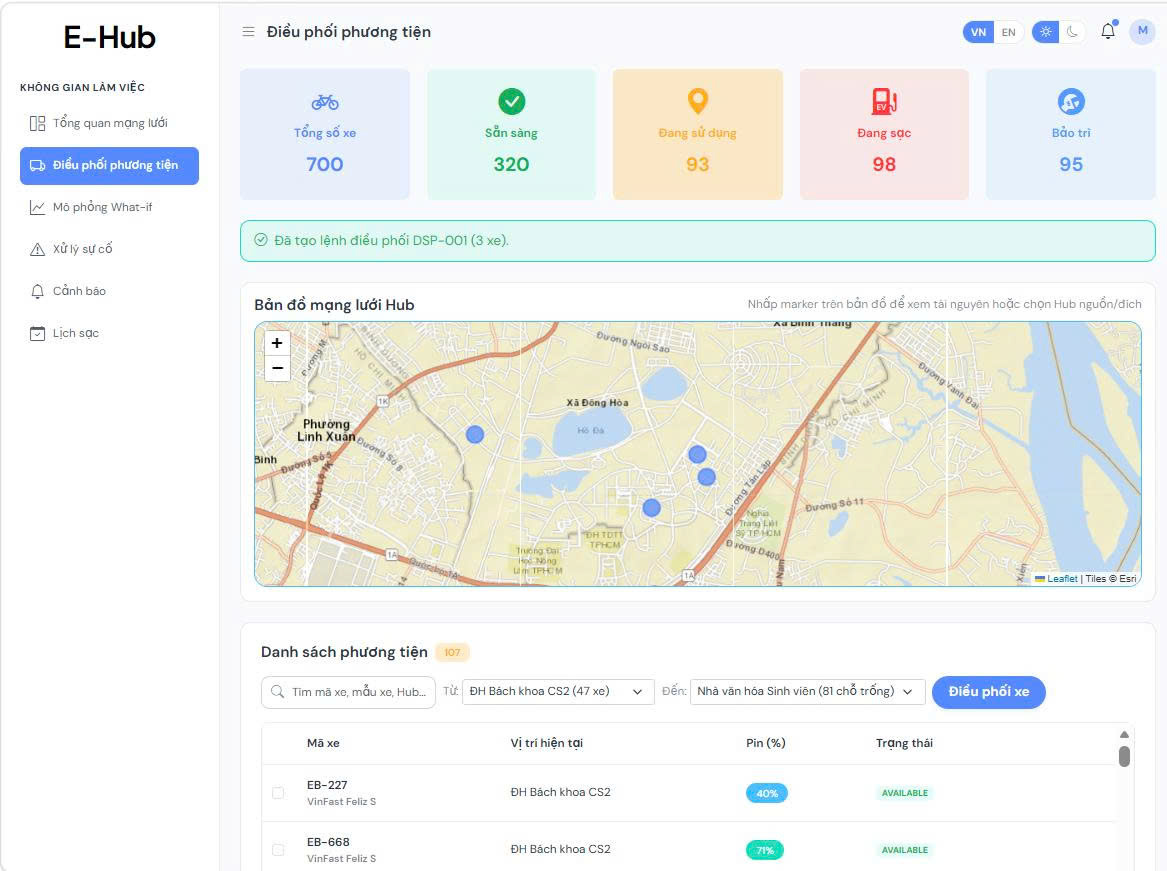
\includegraphics[width=\textwidth]{demo_UC1-17/UC11_dieu_phoi_phuong_tien_3_thanh_cong.jpg}
        \caption{Xác nhận tạo lệnh điều phối thành công}
    \end{subfigure}
    \caption{UC11 --- Quy trình điều phối phương tiện giữa các Hub}
    \label{fig:demo_uc11}
\end{figure}

\paragraph{UC12 --- Xử lý sự cố:}
Ghi nhận, theo dõi danh sách sự cố theo Hub/xe và cập nhật trạng thái xử lý trên màn hình chi tiết sự cố (\texttt{/operator/incidents}).
\begin{figure}[H]
    \centering
    \begin{subfigure}[b]{0.48\textwidth}
        \centering
        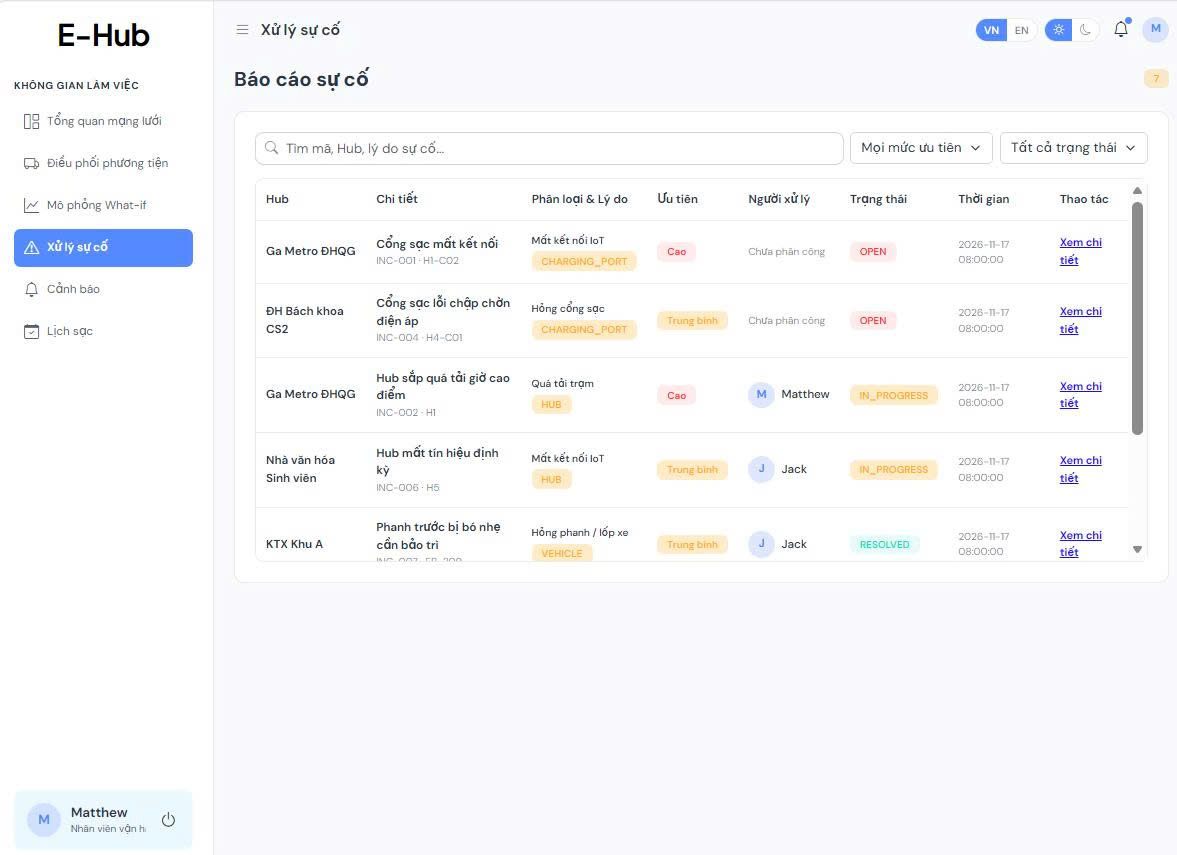
\includegraphics[width=\textwidth]{demo_UC1-17/UC12_xu_ly_su_co_1_danh_sach.jpg}
        \caption{Danh sách sự cố và biểu mẫu ghi nhận nhanh}
    \end{subfigure}
    \hfill
    \begin{subfigure}[b]{0.48\textwidth}
        \centering
        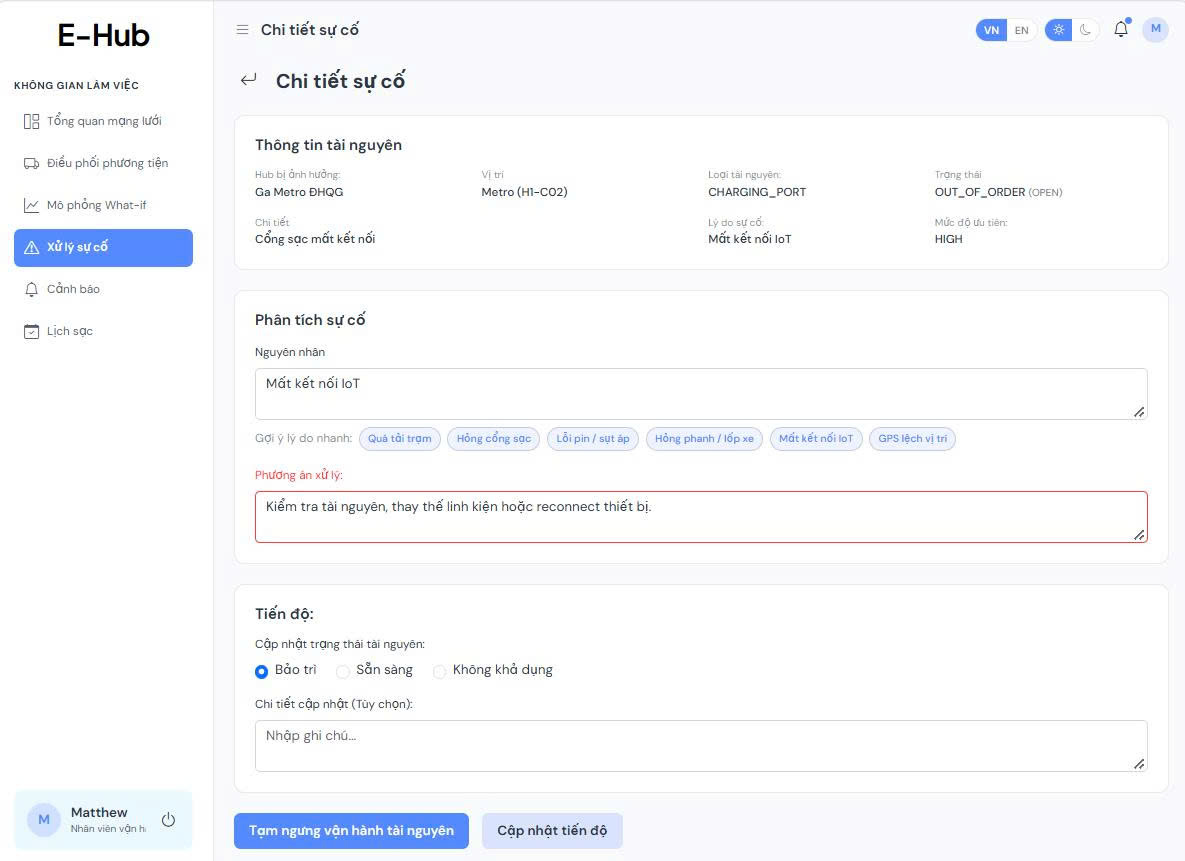
\includegraphics[width=\textwidth]{demo_UC1-17/UC12_xu_ly_su_co_2_chi_tiet.jpg}
        \caption{Chi tiết và thao tác xử lý sự cố}
    \end{subfigure}
    \caption{UC12 --- Quản lý và xử lý sự cố vận hành}
    \label{fig:demo_uc12}
\end{figure}

\paragraph{UC13 --- Lập lịch sạc thông minh:}
Hệ thống tự động đề xuất lịch sạc tối ưu cho các phương tiện pin yếu và cho phép Operator chỉnh sửa, phê duyệt (\texttt{/operator/schedule}).
\begin{figure}[H]
    \centering
    \begin{subfigure}[b]{0.48\textwidth}
        \centering
        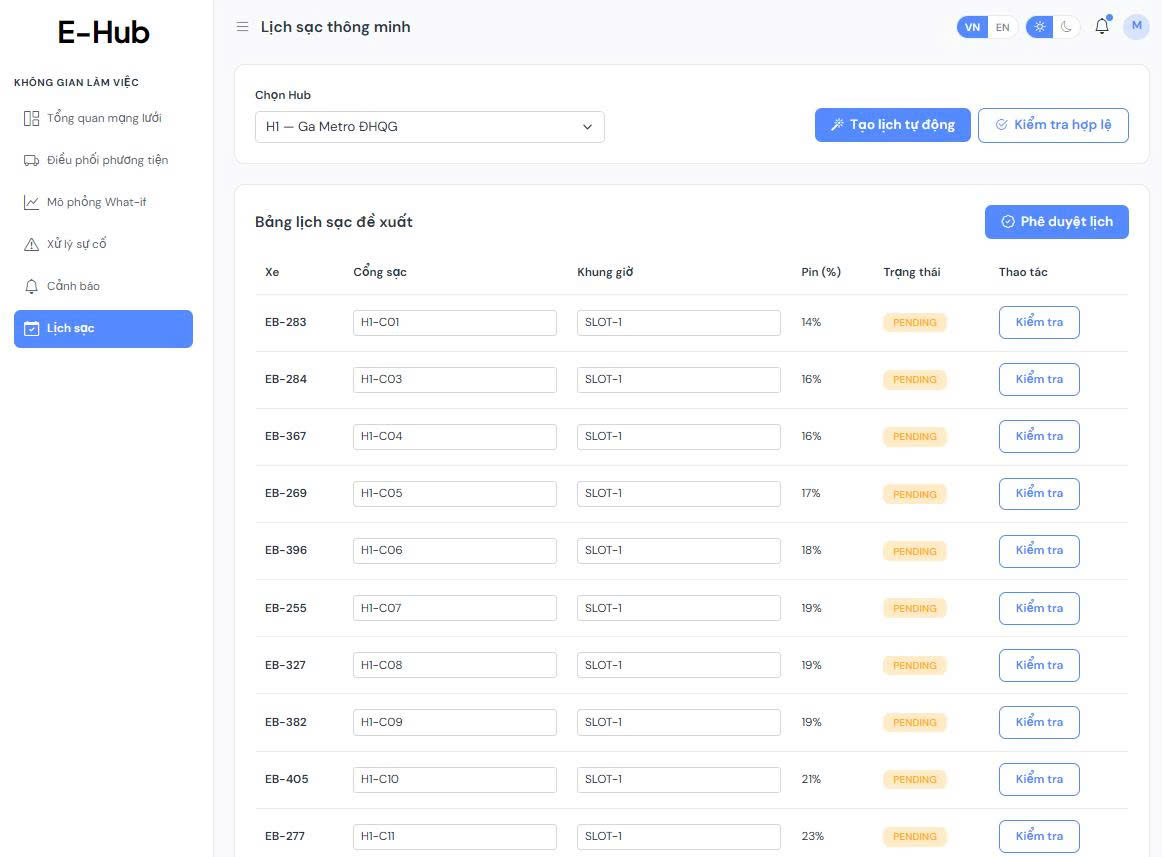
\includegraphics[width=\textwidth]{demo_UC1-17/UC13_lich_sac_thong_minh_1_de_xuat.jpg}
        \caption{Đề xuất lịch sạc theo Hub và mức pin}
    \end{subfigure}
    \hfill
    \begin{subfigure}[b]{0.48\textwidth}
        \centering
        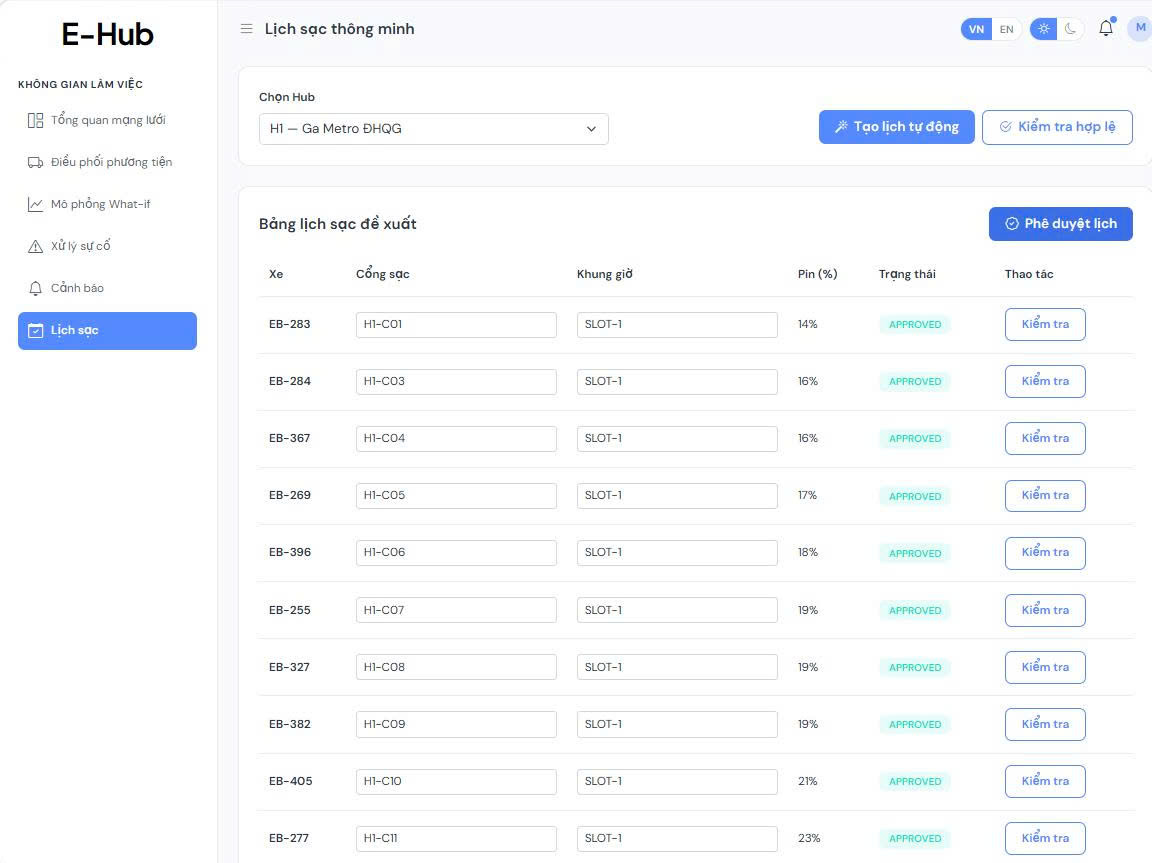
\includegraphics[width=\textwidth]{demo_UC1-17/UC13_lich_sac_thong_minh_2_phe_duyet.jpg}
        \caption{Phê duyệt lịch sạc thành công}
    \end{subfigure}
    \caption{UC13 --- Đề xuất và phê duyệt lịch sạc thông minh}
    \label{fig:demo_uc13}
\end{figure}

\paragraph{UC14 --- Mô phỏng What-if:}
Chạy thử kịch bản thời tiết, khung giờ và tình huống quá tải trên môi trường cô lập, xuất biểu đồ Chart.js và khuyến nghị điều phối mà không làm thay đổi dữ liệu vận hành thật (\texttt{/operator/simulation}).
\begin{figure}[H]
    \centering
    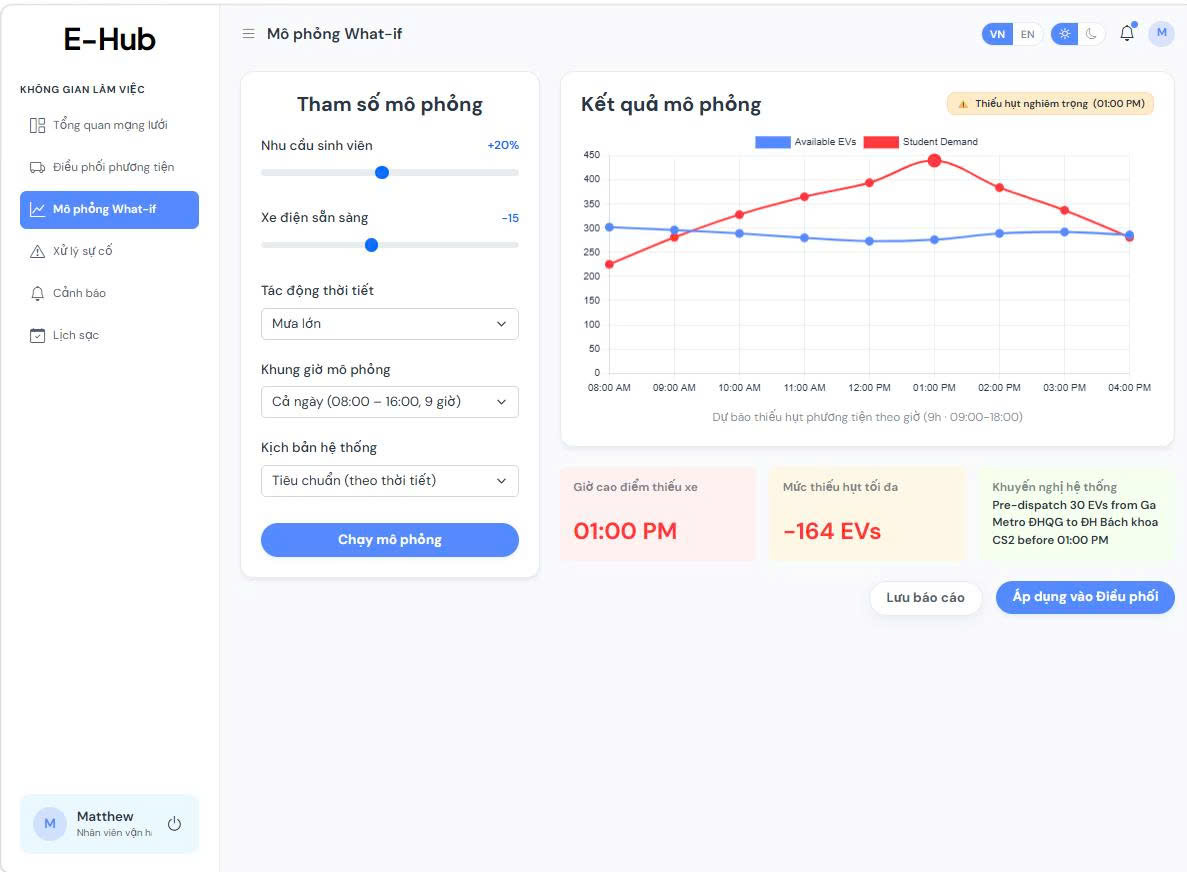
\includegraphics[width=0.88\textwidth]{demo_UC1-17/UC14_mo_phong_what_if.jpg}
    \caption{UC14 --- Kết quả mô phỏng What-if với biểu đồ nhu cầu và nguồn cung}
    \label{fig:demo_uc14}
\end{figure}

\paragraph{UC16 --- Cập nhật trạng thái \& Lọc gói trễ:}
Minh họa demo bắt buộc lọc và loại bỏ gói tin telemetry trễ (\texttt{scripts/packet\_demo.py}), ghi nhận trạng thái \texttt{ACCEPTED}/\texttt{OUTDATED\_IGNORED} vào bảng \texttt{PACKET\_LOG} trên Dashboard.
\begin{figure}[H]
    \centering
    \begin{subfigure}[b]{0.88\textwidth}
        \centering
        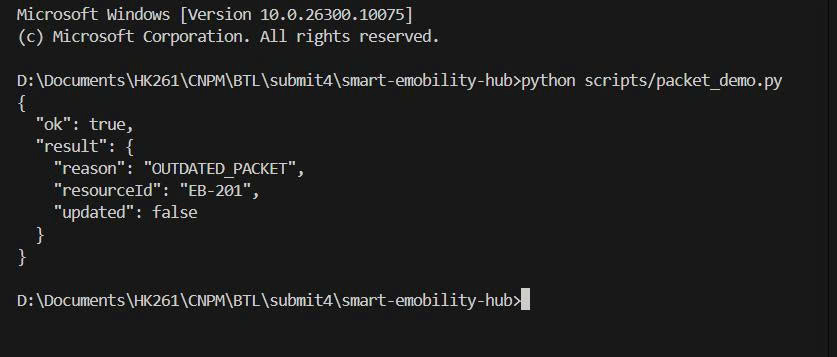
\includegraphics[width=\textwidth]{demo_UC1-17/UC16_cap_nhat_trang_thai_1_terminal.jpg}
        \caption{Kết quả chạy kịch bản demo lọc gói trễ (\texttt{scripts/packet\_demo.py})}
    \end{subfigure}

    \vspace{0.3cm}
    \begin{subfigure}[b]{0.88\textwidth}
        \centering
        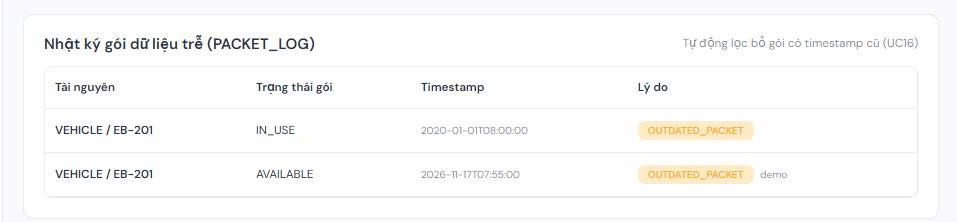
\includegraphics[width=\textwidth]{demo_UC1-17/UC16_cap_nhat_trang_thai_2_packet_log.jpg}
        \caption{Nhật ký gói tin \texttt{PACKET\_LOG} hiển thị trên trang tổng quan Operator}
    \end{subfigure}
    \caption{UC16 --- Cơ chế cập nhật trạng thái thời gian thực và lọc gói dữ liệu trễ}
    \label{fig:demo_uc16}
\end{figure}

\newpage
\section{Tổng kết và Hướng phát triển}

\subsection{Kết quả đạt được}
Nhóm 09 đã hoàn thành bản MVP của hệ thống \textbf{E-Hub} đáp ứng đầy đủ 17 Use Case thiết kế từ Submission 1--3:
\begin{itemize}
    \item Hoàn thiện đầy đủ giao diện Sinh viên (Mobile + Responsive Web) và Dashboard Operator ở cả chế độ Sáng/Tối và song ngữ Việt/Anh (323 khóa).
    \item Hiện thực đầy đủ tầng nghiệp vụ \texttt{services/} và dữ liệu giả lập quy mô 5 Hub, 700 xe, 830 chỗ đỗ, 220 cổng sạc.
    \item Vượt qua toàn bộ \textbf{87/87 test case} tự động trên \texttt{pytest} và chứng minh thành công cả 3 demo bắt buộc (race condition đặt xe, lọc gói trễ, cô lập dữ liệu mô phỏng).
\end{itemize}

\subsection{Bài học kinh nghiệm}
\begin{itemize}
    \item Việc thống nhất hợp đồng dữ liệu (\texttt{DATA\_CONTRACT.md}) ngay từ đầu giúp các thành viên làm giao diện và logic song song mà không bị xung đột tên trường khi tích hợp.
    \item Tách biệt tầng Presentation và Service giúp việc viết kiểm thử tự động (\texttt{pytest}) nhanh chóng và cô lập lỗi hiệu quả.
    \item \textit{\_TODO: Bổ sung thêm bài học kinh nghiệm sau buổi họp tổng kết và quay demo của nhóm.\_}
\end{itemize}

\subsection{Hướng phát triển}
\begin{itemize}
    \item Chuyển đổi dữ liệu giả lập \texttt{seed.json} sang hệ quản trị cơ sở dữ liệu thực tế (PostgreSQL/Redis) và sử dụng WebSocket thay cho cơ chế polling mỗi 5 giây.
    \item Tích hợp xác thực SSO thực tế của ĐHQG-HCM và kết nối luồng telemetry từ thiết bị GPS/IoT gắn trên phương tiện.
\end{itemize}

\newpage

%%%%%%%%%%%%%%%%% OUTRO %%%%%%%%%%%%%%%%%%%
\section*{Tài liệu tham khảo}
\addcontentsline{toc}{section}{Tài liệu tham khảo}

\begin{enumerate}
    \item Tài liệu hướng dẫn và đặc tả Bài tập lớn môn Công nghệ Phần mềm (CO3001), Khoa Khoa học và Kỹ thuật Máy tính, Trường Đại học Bách khoa --- ĐHQG-HCM, Học kỳ HK261.
\end{enumerate}

\newpage
\section*{Phụ lục: Khai báo sử dụng Generative AI}
\addcontentsline{toc}{section}{Phụ lục: Khai báo sử dụng Generative AI}

Theo yêu cầu minh bạch của môn học, bảng dưới đây tổng hợp việc sử dụng công cụ Generative AI của các thành viên trong Nhóm 09 (cập nhật từ tệp \texttt{docs/AI\_USAGE.md}).

\begin{longtable}{|p{2.3cm}|p{2.1cm}|p{3.0cm}|p{2.5cm}|p{3.5cm}|}
\caption{Bảng khai báo sử dụng Generative AI của Nhóm 09} \\
\hline
\textbf{Thành viên} & \textbf{Công cụ} & \textbf{Dùng cho phần nào} & \textbf{Mức độ đóng góp} & \textbf{Nhóm đã tự chỉnh sửa, kiểm tra gì} \\
\hline
\endfirsthead
\hline
\textbf{Thành viên} & \textbf{Công cụ} & \textbf{Dùng cho phần nào} & \textbf{Mức độ đóng góp} & \textbf{Nhóm đã tự chỉnh sửa, kiểm tra gì} \\
\hline
\endhead
TV1 (Nguyễn Khang Kỳ) & \textit{\_TODO\_} & \textit{\_TODO\_} & \textit{\_TODO\_} & \textit{\_TODO\_} \\ \hline
TV2 (Châu Mạnh Phát) & \textit{\_TODO\_} & \textit{\_TODO\_} & \textit{\_TODO\_} & \textit{\_TODO\_} \\ \hline
TV3 (Hoàng Phạm Tiến Thành) & Claude \& agent lập trình & Gợi ý phân công nhóm, dựng khung Flask MVP, viết prompt dựng giao diện Dashboard từ mockup Figma & Gợi ý ý tưởng, viết nháp, sinh code màn hình Dashboard & Tự chạy thử test/server xác nhận khung code chạy đúng, tự chốt nhãn hiển thị/nút bấm, đối chiếu với mockup gốc \\ \hline
TV4 (Võ Tấn Phát) & ChatGPT, Claude & Gợi ý test case cho Submission 3 và kiểm tra lỗi code & Gợi ý ý tưởng, kiểm tra lỗi & Kiểm tra lại tính phù hợp của test case, tự sửa lỗi code bằng tay \\ \hline
TV5 (Đào Huy Phong) & \textit{\_TODO\_} & \textit{\_TODO\_} & \textit{\_TODO\_} & \textit{\_TODO\_} \\ \hline
\end{longtable}

\end{document}
